\documentclass[11pt]{article}
\usepackage[utf8]{inputenc}
\usepackage{amsmath,amsthm,amsfonts,amssymb,amscd}
\usepackage{multirow,booktabs}
\usepackage[table]{xcolor}
\usepackage{fullpage}
\usepackage{cancel}
\usepackage{lastpage}
\usepackage{physics}
\usepackage{enumitem}
\usepackage{fancyhdr}
\usepackage{simpler-wick}
\usepackage{mathrsfs}

\usepackage{wrapfig}
\usepackage{tikz}
\usepackage{tikz-feynman}
\usepackage{setspace}
\usepackage{calc}
\usepackage{multicol}
\usepackage{cancel}
\usepackage[retainorgcmds]{IEEEtrantools}
\usepackage[margin=3cm]{geometry}
\usepackage{amsmath}
\newlength{\tabcont}
\setlength{\parindent}{0.0in}
\setlength{\parskip}{0.05in}
\usepackage{empheq}
\usepackage{framed}
\usepackage[most]{tcolorbox}
\usepackage{xcolor}
\usepackage{tcolorbox}
\usepackage{slashed}
\usepackage{dsfont}
\colorlet{shadecolor}{orange!15}
\parindent 0in
\parskip 12pt
\geometry{margin=1in, headsep=0.25in}
\theoremstyle{definition}
\newtheorem{defn}{Definition}
\newtheorem{reg}{Rule}
\newtheorem{exer}{Exercise}
\newtheorem{note}{Note}
\usetikzlibrary{arrows.meta}
\usetikzlibrary{patterns.meta, positioning, shapes.geometric}
\allowdisplaybreaks[4]
\usepackage[utf8]{inputenc}
\usepackage{titlesec}

\usepackage[colorlinks=true, linkcolor=blue, urlcolor=blue, citecolor=blue]{hyperref}
\titleformat{\section}{\Large\bfseries}{\thesection}{1em}{}
\titleformat{\subsection}{\large\bfseries}{\thesubsection}{1em}{}


\begin{document}
\title{Quantum Field Theory}


\thispagestyle{empty}

\begin{titlepage}
\centering



\vspace*{3cm} % 顶部留白

% 标题
{\fontsize{38}{46}\selectfont\bfseries Quantum Field Theory}

\vspace{1.5cm} % 标题与作者间距

% 作者
{\Large \itshape Luca Jin}

\vspace{0.5cm} % 作者与年份间距

% 年份
{\large 2025}

\vfill % 填充剩余空间



\end{titlepage}

\tableofcontents
\newpage

{\LARGE \bf Quantum Field Theory}


\section{Classical Field Theory}
\subsection{The Euler-Lagrange Equations}
The action $S$ is defined as 
\begin{equation}
    S = \int dt L = \int d^4x \mathcal{L},
\end{equation}
where $L$ is the Lagrangian of the system, and $\mathcal{L}$ is the Lagrangian density. Say we have a Lagrangian $\mathcal{L}[\phi, \partial_\mu\phi]$ is only a functional of $\phi$ and $\partial_\mu\phi$. Then,
\begin{equation}
    \begin{aligned}
        \delta S &= \int d^4x \biggr [ \frac{\partial\mathcal{L}}{\partial \phi}\delta\phi + \frac{\partial\mathcal{L}}{\partial(\partial_\mu\phi)}\delta(\partial_\mu\phi)\biggr] \\
        & = \int d^4x\biggr\{  \biggr(\frac{\partial\mathcal{L}}{\partial \phi} - \frac{\partial\mathcal{L}}{\partial(\partial_\mu\phi)}\biggr)\delta\phi  + \partial_\mu\biggr[\frac{\partial\mathcal{L}}{\partial(\partial_\mu\phi)}\delta(\phi)\biggr] \biggr\}.
        \label{Eq. EL derivation}
    \end{aligned}
\end{equation}
The last term is a total integral and the boundary condition will always force it to vanish. Imposing the principal of least action, $\frac{\delta S}{\delta\phi} =0$. Hence, this implies
\begin{shaded}
    \begin{equation}
        \frac{\partial\mathcal{L}}{\partial \phi} - \frac{\partial\mathcal{L}}{\partial(\partial_\mu\phi)} = 0.
    \end{equation}
\end{shaded}
\subsection{Noether's Theorem}
A Lagrangian may be invariant under some transformation $\phi \rightarrow \phi + \delta\phi$, which is called a symmetry. When there is such a symmetry that depends on some parameter $\alpha$ that can be taken small (a continuous symmetry), we find, similar to (\ref{Eq. EL derivation})
\begin{equation}
    0 = \frac{\delta \mathcal{L}}{\delta \alpha} = \sum _n \biggr(\frac{\partial\mathcal{L}}{\partial \phi_n} - \frac{\partial\mathcal{L}}{\partial(\partial_\mu\phi_n)}\biggr)\frac{\delta\phi_n}{\delta\alpha}  + \partial_\mu\biggr[\frac{\partial\mathcal{L}}{\partial(\partial_\mu\phi_n)}\frac{\delta\phi_n}{\delta\alpha}\biggr].
    \label{N1}
\end{equation}
When the equation of motion is satisfied, then (\ref{N1}) simplifies to $\partial_
\mu J^\mu = 0$ with
\begin{shaded}
\begin{equation}
    J^\mu = \sum_n \frac{\partial\mathcal{L}}{\partial(\partial_\mu\phi_n)}\frac{\delta\phi_n}{\delta\alpha}.
\end{equation}
\end{shaded}
This is known as the Noether current.
Such a vector field is also called a conserved current, since the total charge $Q$, defined as 
\begin{equation}
    Q = \int d^3xJ_0,
\end{equation}
satisfies
\begin{equation}
    \partial_tQ = \int d^3x\partial_tJ_0 = \int d^3x\vec{\nabla}\cdot\vec{J} = \int \vec{dS}\cdot\vec{J} = 0.
\end{equation}
\subsubsection{Energy-Momentum Tensor}
In this section, we will investigate the conserved current corresponding to space-time translation invariance, known as the energy-momentum tensor, $\mathcal{T}_{\mu\nu}$. Now, let us consider the transformation $y^\mu \rightarrow y^\mu - \xi^\mu$ with $\xi^\mu$ to be a constant four-vector. The scalar fields then would transform as $\phi(x) \rightarrow \phi(x+\xi)$. For infinitesimal $\delta\xi^\mu$
\begin{equation}
    \phi(x) \rightarrow \phi(x+\delta\xi)= \phi(x) + \delta\xi^\mu\partial_\mu\phi(x)+\cdots.
    \end{equation}
This implies
\begin{equation}
    \frac{\delta\phi(x)}{\delta\xi^\mu} = \partial_\mu\phi(x).
\end{equation}
As the Lagrangian is also a function of $x$, we have
\begin{equation}
    \frac{\delta\mathcal{L}}{\delta\xi^\mu} = \partial_\mu\mathcal{L}.
\end{equation}
Since this is a total derivative, $\delta S = \int d^4x \delta\mathcal{L}=\delta\xi^\mu\int d^4x \partial_\mu\mathcal{L}=0$, which is why we sometimes say this is a symmetry of the action, not the Lagrangian.
Similarly to before, we have
\begin{equation}
    \frac{\delta\mathcal{L}[\phi_n,\partial_\mu\phi_n]}{\delta\xi^\nu} = \partial_\mu\sum _n\biggr [\frac{\partial\mathcal{L}}{\partial(\partial_\mu\phi_n)}\frac{\delta\phi_n}{\delta\xi^\nu} \biggr] = \partial_\mu\sum _n\biggr[\frac{\partial\mathcal{L}}{\partial(\partial_\mu\phi_n)}\partial_\nu\phi_n(x)\biggr].
\end{equation}
Thus, 
\begin{equation}
\begin{aligned}
        \partial_\nu\mathcal{L}-\partial_\mu\sum _n\biggr[\frac{\partial\mathcal{L}}{\partial(\partial_\mu\phi_n)}\partial_\nu\phi_n(x)\biggr] = 0 \\
        \implies \partial_\mu \biggr(\sum _n\frac{\partial\mathcal{L}}{\partial(\partial_\mu\phi_n)}\partial_\nu\phi_n - g_{\mu\nu}\mathcal{L}\bigg)=0.
\end{aligned}
\end{equation}
We obtained a conserved current with four components, being energy and momentum. Therefore, we define the energy-momentum tensor $\mathcal{T}_{\mu\nu}$ to be
\begin{shaded}
    \begin{equation}
        \mathcal{T}_{\mu\nu} = \sum _n\frac{\partial\mathcal{L}}{\partial(\partial_\mu\phi_n)}\partial_\nu\phi_n - g_{\mu\nu}\mathcal{L}
    \end{equation}
\end{shaded}
with $\partial_\mu\mathcal{T}_{\mu\nu} = 0$.

\subsection{Green's Functions}
Now, we will introduce a very powerful tool in field theory,  the Green's functions. Suppose we have a very general differential equation formed from a linear operator $\hat{L}$
\begin{equation}
    \hat{L}x(t) = f(t).
\end{equation}
The Green's function $G(t, u)$ (or $\Pi(t, u)$) of the equation is defined as
\begin{equation}
    \hat{L}G(t,u) = \delta(t-u).
\end{equation}
\begin{tcolorbox}[breakable, colback=yellow!20!white, colframe=black, boxrule=1pt]
Let us consider a familiar example from mechanics. We will ltake an oscillator of mass $m$ and spring constant $K$ evolving under the influence of a time-dependent force $f(t)$. The equation of motion for this is

\begin{equation}
m\frac{d^{2}}{dt^{2}}x(t) + Kx(t) = f(t), 
\end{equation}

so here the linear operator is $\hat{L} = m\frac{d^{2}}{dt^{2}} + K$. We can build up a force function $f(t)$ by adding together lots of delta functions.

\begin{equation}
f(t) = \int_{0}^{\infty} du\, f(u)\delta(t-u),
\end{equation}

where $u$ is a dummy variable which allows us to break $f(t)$ into deltas. This is, of course, merely an example of superposition and is allowed because our differential equation is linear.

Instead of hitting the problem head-on, we sidestep and solve Eq.~(16.3) for just one of the delta functions. We'll call this solution the Green's function $G(t,u)$:

\begin{equation}
\left[m\frac{d^{2}}{dt^{2}} + K\right]G(t,u) = \delta(t-u).
\end{equation}

The complete solution to Eq.~(16.3) is then given by the integral of the Green's function, weighted by the force function $f(u)$:

\begin{equation}
x(t) = \int_{0}^{\infty} du\, G(t,u)f(u).
\end{equation}

The solution is therefore simply a sum of the responses of the system in $x$ to the stimuli $f(u)$.

Why is the solution to Eq.~(16.3) given by Eq.~(16.6)? Start by acting on Eq.~(16.6) with the operator $\hat{L}$ (which passes through the integral sign on the right-hand side),

\begin{align}
\hat{L}\,x(t) &= \int du\, \hat{L}\,G(t,u)f(u) \notag \\
&= \int du\, \delta(t-u)f(u)  \\
&= f(t) 
\end{align}

which is where we started! This implies we can solve an inhomogeneous differential equation by finding the Green's function $G(t,u)$ and then integrating over $f(u)$ to get the solution $x(t)$.


\end{tcolorbox}

\section{Second Quantization}
\subsection{Quantum Mechanical Harmonic Oscillator}
The classical Hamiltonian of a simple harmonic oscillator system is given by
\begin{equation}
    H = \frac{p^2}{2m} + \frac{1}{2}m\omega^2x^2
    \label{Eq.Simple Harmonic Oscillator Hamiltonian}.
\end{equation}
To quantize a classical system, we introduce the commutation relation:
\begin{equation}
    [x, p] = i.
    \label{Eq.QM commutation relation}
\end{equation}
To simplify, we change the variables to 
\begin{equation}
    a = \sqrt{\frac{m\omega}{2}}(x + \frac{ip}{x\omega}), a^{\dagger} = \sqrt{\frac{m\omega}{2}}(x - \frac{ip}{x\omega}),
    \label{Eq.Creation and Annihilation}
\end{equation}
which satisfies
\begin{equation}
    [a, a^{\dagger}] = 1,
\end{equation}
and hence
\begin{equation}
    H = \omega(a^{\dagger}a + \frac{1}{2}).
\end{equation}
In the Heisenberg picture, the equation of motion is given by
\begin{equation}
    i\frac{d}{dt}a = [a, H] = \omega a,
\end{equation}
and the solution to this equation is 
\begin{equation}
    a(t) = ae^{-i\omega t}.
\end{equation}
Therefore, the position of the particle $x$ is given by
\begin{equation}
    x(t) = ae^{-i\omega t} + a^\dagger e^{i\omega t}.
\end{equation}

If we have $N$ such uncoupled oscillators, the Hamiltonian becomes
\begin{equation}
    H = \sum_i \frac{p_i^2}{2m_i} + \frac{1}{2}m\omega_i^2x_i^2.
\end{equation}
As the particles are not coupled, the commutation relation can be modified as
\begin{equation}
    [x_i, p_i] = i\delta_{ij},
\end{equation}
and hence
\begin{equation}
    [a_i, a_j^\dagger] = \delta_{ij}.
    \label{Eq. QM commutation}
\end{equation}
Following the steps above, the centre of mass of the system can be obtained to be
\begin{equation}
    x(t) = \sum_i  a_ie^{-i\omega t} + a_i^\dagger e^{i\omega t}.
    \label{Eq. CoM}
\end{equation}
\subsection{Second Quantization}
\subsubsection{The Klein-Gordon Equation}
To obtain a relativistic theory, we require the Hamiltonian to be Lorentz invariant. Recall the energy-momentum relation: 
\begin{equation}
    \omega^2 = m^2 + \vec{p}^2.
\end{equation}
By substituting $\vec{p} \rightarrow -i\vec{\nabla}$ and $E \rightarrow i\partial_t$, and multiplying both sides by a field $\phi$ (just as in quantum mechanics), we obtained a relativistic equation of motion known as the Klein-Gordon equation
\begin{shaded}
    \begin{equation}
        (\square + m^2)\phi(\vec{x}, t) = 0.
    \end{equation}
\end{shaded}

To solve this equation, we first define $\tilde{\phi}(p)$ to be the Fourier transform of $\phi(x)$:
\begin{equation}
    \phi(\vec{x}, t) = \int \frac{d^3p}{(2\pi)^3} \tilde{\phi}(\vec{p}, t)e^{i\vec{p}  \vec{x}}.
\end{equation}
Thus,
\begin{equation}
    (\partial_t^2  + \vec{p}^2+m^2)\tilde{\phi}(\vec{p}, t)e^{i\vec{p}\vec{x}} = 0 \\
    \implies \partial_t^2 \tilde{\phi}(\vec{p}, t) = -\omega^2.
\end{equation}
Hence, we have
\begin{equation}
    \tilde{\phi}(\vec{p}, t)  = a_pe^{-i\omega t}e^{-i\vec{p}\vec{x}} = a_pe^{-ipx}.
\end{equation}
Another solution would be
\begin{equation}
    \tilde{\phi}(\vec{p}, t)  = b_pe^{ipx}.
\end{equation}
Therefore, $\phi(x)$ should be the linear combination of them:
\begin{equation}
    \phi(x) = \int \frac{d^3p}{(2\pi)^3} (a_pe^{-ipx} + b_pe^{ipx}).
\end{equation}
If we force $\phi$ to be real, we need $b = a^*$, which gives
\begin{equation}
    \phi(x) = \int \frac{d^3p}{(2\pi)^3} (a_pe^{-ipx} + a_p^*e^{ipx}).
    \label{Eq. phi classic}
\end{equation}
One would also notice that the Lagrangian
\begin{equation}
    L = \int d^3 x \left[-\frac{1}{2}\phi (\square + m^2)\phi \right] = \int d^3 x \left[\frac{1}{2}(\partial_\mu \phi)^2 - \frac{1}{2}m^2\phi^2 \right] 
\end{equation}
reproduces the Klein-Gordon equation. Therefore, the Hamiltonian would be
\begin{equation}
    H = \int d^3x \left[\frac{1}{2}(\partial_t \phi)^2 + \frac{1}{2}\nabla^2\phi + \frac{1}{2}m^2\phi^2\right].
\end{equation}
\subsubsection{Quantizing Klein-Gordon Equation}
In the last section, we have solved the Klein-Gordon equation classically. Now, we want to turn it into a quantum theory. One would observe that (\ref{Eq. phi classic}) is the continuum limit of (\ref{Eq. CoM}). Therefore, it is natural to modify the commutation relation in (\ref{Eq. QM commutation}) by turning the Kronecker delta $\delta_{ij}$ into the Dirac delta function $\delta^3(\vec{p}-\vec{q})$ up to a normalisation factor:
\begin{equation}
    [a_p, a_p^\dagger] = \mathcal{N}\delta^3(\vec{p}-\vec{q}).
\end{equation}
Just as in quantum mechanics, these operators create and annihilate particles with momentum $\vec{p}$:
\begin{equation}
    a_p^\dagger \ket{0} = \frac{1}{\sqrt{2\omega_p}}\ket{p}, a_p\ket{p} = \frac{1}{\sqrt{2\omega_p}}\ket{0},
\end{equation}
where $\omega_p = \sqrt{\vec{p}^2 + m^2}$ is the on-shell energy of the particle with momentum $\vec{p}$.
To compute the normalisation, we start by defining 
\begin{equation}
    \braket{0}{0} =  1.
\end{equation}
Therefore, 
\begin{shaded}
\begin{equation}
    \braket{q}{p} = \sqrt{2\omega_p}\sqrt{2\omega_q}\bra{0}a_q a_p^\dagger\ket{0} = 2\omega_p (2\pi)^3\delta^3(\vec{p}-\vec{q}).
\end{equation}
\end{shaded}
The identity operator for a one-particle state is 
\begin{equation}
    \mathds{1} = \int \frac{d^3p}{(2\pi)^3} \frac{1}{\sqrt{2\omega_p}}\ket{p}\bra{p},
\end{equation}
which we can check by 
\begin{equation}
    \ket{k} = \int \frac{d^3p}{(2\pi)^3} \frac{1}{2\omega_p}\ket{p}\braket{p}{k} = \int d^3p   \delta^3(\vec{p}-\vec{q})\ket{p} = \ket{k}
\end{equation}
\begin{tcolorbox}[breakable, colback=yellow!20!white, colframe=black, boxrule=1pt]
Let us investigate the Lorentz transformation property. First, note that 
\begin{equation}
    \int d^4k
\end{equation}
is Lorentz-invariant.
One can also prove the following:

\begin{align*}
    \int dk^0 \delta(k^2 - m^2) \theta(k^0) & = \int dk^0 \delta((k^0)^2 - \omega_k^2) \theta(k^0) \\
    & =\int^\infty_{-\infty} dk^0 \frac{1}{2\abs{\omega_k}}[\delta(k^0 + \omega_k) + \delta(k^0 - \omega_k)]\theta(k^0) \\
    & =\int^\infty_0 dk^0 \frac{1}{2\abs{\omega_k}}[\delta(k^0 + \omega_k) + \delta(k^0 - \omega_k)] \\
    & =\int^\infty_{-\infty} dk^0 \frac{1}{2\abs{\omega_k}}\delta(k^0 - \omega_k) \\
    & = \frac{1}{2\omega_k}.
\end{align*}
Hence,
\begin{equation}
    \int d^4k = \int \frac{d^3k}{2\omega_k}
\end{equation}
is Lorentz-invariant, where we have suppressed the additional factor $\delta(k^2 - m^2) \theta(k^0)$.
\end{tcolorbox}
Now, we will define the free scalar field operator $\phi_0(x)$ to be
\begin{shaded}
    \begin{equation}
        \phi_0(x) = \int \frac{d^3p}{(2\pi)^3} \frac{1}{\sqrt{2\omega_p}}(a_pe^{-ipx} + a_p^\dagger e^{ipx}).
    \end{equation}
\end{shaded}

\begin{tcolorbox}[breakable, colback=yellow!20!white, colframe=black, boxrule=1pt]
$\phi_0(x)$ can be rewritten as 
\begin{equation}
    \phi_0(x) = \int \frac{d^3p}{(2\pi)^3} \frac{1}{2\omega_p}(\sqrt{2\omega_p}a_pe^{-ipx} + \sqrt{2\omega_p}a_p^\dagger e^{ipx}).
\end{equation}
Recall that $\ket{p}=\sqrt{2\omega_p}a_p^\dagger\ket{0}$ and $\int \frac{d^3k}{2\omega_k}$ are Lorentz-invariant, and hence $\phi_0(x)$ is also Lorentz-invariant.
\end{tcolorbox}

To make sense of the free scalar field operator $\phi_0(x)$, we can act it on a vacuum state and project it onto a momentum component
\begin{align*}
    \bra{q}\phi_0(x)\ket{0} & = \int \frac{d^3p}{(2\pi)^3} \frac{1}{\sqrt{2\omega_p}}\bra{q}\frac{1}{\sqrt{2\omega_p}}e^{ipx}\ket{p} \\
& = e^{iqx} \\
& = \braket{q}{x}.
\end{align*}
Therefore, the field operator creates a particle at a space-time position $x$.
Occasionally, we would also need the equal-time commutation relations. The commutator of two fields at two different space-time positions is given by
\begin{equation}
\begin{aligned}
\left[\phi_0(x), \phi_0(y) \right] &= \int \frac{d^3p}{(2\pi)^3} \int \frac{d^3q}{(2\pi)^3} \frac{1}{\sqrt{2\omega_p 2\omega_q}} \biggl\{ \cancel{[a_p, a_q]e^{-i(px+qy)}} + [a_p, a_q^\dagger]e^{-i(px-qy)} \\
&\qquad \qquad \qquad \qquad + [a_p^\dagger, a_q]e^{-i(-px+qy)} + \cancel{[a_p^\dagger, a_q^\dagger]e^{i(px+qy)}} \biggr\} \\
&= \int \frac{d^3p}{(2\pi)^3} \int d^3q \, \frac{1}{\sqrt{2\omega_p 2\omega_q}}\delta^3(\vec{p}-\vec{q}) \biggl\{ e^{-i(px-qy)} - e^{-i(-px+qy)} \biggr\}.
\end{aligned}
\end{equation}
For equal-time commutation relations, $x^0 = y^0$, and hence,
\begin{shaded}
    \begin{equation}
        \left[\phi_0(\vec{x}), \phi_0(\vec{y}) \right] = \int \frac{d^3p}{(2\pi)^3} \frac{1}{2\omega_p}\biggl\{e^{i\vec{p}(\vec{x}-\vec{y})} - e^{-i\vec{p}(\vec{x}-\vec{y})} \biggr\} = 0.
    \end{equation}
    \label{Eq. E-T 1}
\end{shaded}
Next, we define the time derivative operator (canonical momentum operator) $\pi$ to be
\begin{equation}
    \pi(x) = \partial_t\phi(x) = -i\int \frac{d^3p}{(2\pi)^3} \sqrt{\frac{\omega_p}{2}}(a_pe^{i\vec{p}\vec{x}} - a_p^\dagger e^{-i\vec{p}\vec{x}}).
\end{equation}
Now we compute
\begin{equation}
\begin{aligned}
    \left[\phi(x), \pi(y)\right] &= -i\int \frac{d^3p}{(2\pi)^3} \int \frac{d^3q}{(2\pi)^3} \frac{1}{2} \biggl\{ \cancel{[a_p, a_q]e^{-i(px+qy)}} + [a_p, a_q^\dagger]e^{-i(px-qy)} \\
&\qquad \qquad \qquad \qquad - [a_p^\dagger, a_q]e^{-i(-px+qy)} - \cancel{[a_p^\dagger, a_q^\dagger]e^{i(px+qy)}} \biggr\} \\
&= \frac{i}{2}\int \frac{d^3p}{(2\pi)^3}\delta^3(\vec{p}-\vec{q}) \biggl\{ e^{-i(px-qy)} + e^{-i(-px+qy)} \biggr\}.
\end{aligned}
\end{equation}
Similarly, imposing the equal-time condition, we have,
\begin{shaded}
    \begin{equation}
        \left[\phi(\vec{x}), \pi(\vec{y})\right] = i\int \frac{d^3p}{(2\pi)^3} \biggl\{e^{i\vec{p}(\vec{x}-\vec{y})} + e^{-i\vec{p}(\vec{x}-\vec{y})} \biggr\} = i\delta^3(\vec{x}-\vec{y}).
    \end{equation}
    \label{Eq. E-T 2}
\end{shaded}


\section{Cross Sections and Decay Rates}
\subsection{$S$-matrix}
The $S$-matrix or the scattering matrix is defined as
\begin{equation}
    \bra{f}S\ket{i}_{\text{Heisenberg}} = \braket{f;\infty}{i;\infty}_{\text{Schrödinger}}.
\end{equation}
The $S$-matrix is defined assuming that all of the things that change the state (the interactions) happen in a finite time interval, so that at asymptotic times, $t=\pm \infty$, the state is free of interactions. These free states at $t = \pm \infty$ is called the asymptotic states.
\subsection{Cross Sections}
A cross section is a natural quantity to measure. Classically, it is simply the cross-sectional area of a particle. For example, in the Rutherford gold foil experiment, he was interested in the radius of the nucleus. By colliding the gold foil with beams of $\alpha$-particles, he was able to measure the cross-sectional, $\sigma = \pi r^2$. Now, suppose there was just a single nucleus, then the cross-sectional area is given by
\begin{equation}
\begin{aligned}
    \sigma &= \frac{\text{number of particle scattered}}{\text{total number of particles}}\times\text{area}\\
    &=\frac{\text{number of particle scattered}}{\text{time}\times\text{number density in the beam}\times\text{velocity of the beam}}\\
    &=\frac{1}{T\Phi}N,
\end{aligned}
\end{equation}
where $T$ is the time of the experiment, $N$ is the number of scattered particles, and $\Phi$ is the incoming flux (number density $\times$ velocity of the beam).

It is also natural to measure the diffraction cross section, $\frac{d\sigma}{d\Omega}$, which gives the number of particles scattered in a certain solid angle. 

In quantum mechanics, we generalise the notion of cross-sectional area to cross section with a more abstract meaning as a measure of the interaction strength. In quantum mechanics, a particle has a probability to be scattered or not. Classically, the scatter probability can be written as $P = N/N_{inc}$, where $N_{inc}$ is the number of incoming particles. Therefore, the natural generalisation of this to quantum mechanics would be
\begin{equation}
    d\sigma = \frac{1}{T\Phi/N_{inc}}dP=\frac{1}{T\Phi'}dP,
\end{equation}
where $\Phi'=\Phi/N_{inc}$ is the normalised flux as if the beam has just one particle. From now on, we will be using $\Phi$ to denote the normalised flux.
Now, let us relate the differential cross section to $S$-matrix elements. Practically, it is only possible for two particles to collide at a time. Thus, we will be focusing on the 2 $\rightarrow n$ process:
\begin{equation}
    p_1 + p_2 \rightarrow \{p_j\}.
\end{equation}
In the rest frame of one of the colliding particles, the flux is just the velocity of incoming particle divided by the total volume: $\Phi = \abs{\vec{v}}/V$. In the centre of mass frame, beams of particles come from both sides, and hence $\vec{v} \rightarrow \vec{v_1}- \vec{v_2}$ for $\Phi$. Thus, 
\begin{equation}
    d\sigma = \frac{V}{T\abs{\vec{v_1} - \vec{v_2}}} dP.
\end{equation}
Quantum field theory is essentially just quantum mechanics with an infinite number of fields. Then the  normalised differential probability is 
\begin{equation}
    dP = \frac{\abs{\bra{f}S\ket{i}}^2}{\braket{f}{f}\braket{i}{i}}d\Pi.
\end{equation}
Here, $d\Pi$ is the region of final state momenta at which we are looking. It is defined to be
\begin{equation}
    d\Pi = \prod_j \frac{V}{(2\pi)^3}d^3p_j,
    \label{Eq. dPi}
\end{equation}
so that $\int d\Pi = 1$, since $\int \frac{d^3p}{(2\pi)^3} = \frac{1}{V}$, which does not change the normalisation.
Now, let us evaluate $\braket{f}{f}$ and $\braket{i}{i}$. First recall,
\begin{equation}
    \braket{p}{p}= (2\pi)^3(2\omega_p)\delta^3(0).
\end{equation}
$\delta^3(0)$ is infinite, but it can be understood by the following relation
\begin{equation}
    \delta^3(\vec{p})=\int \frac{d^3x}{(2\pi)^3} e^{i\vec{p}\vec{x}}.
\end{equation}
Hence,
\begin{equation}
    \delta^3(0)=\int \frac{d^3x}{(2\pi)^3} = \frac{V}{(2\pi)^3},
\end{equation}
and similarly,
\begin{equation}
    \delta^4(0) = \frac{TV}{(2\pi)^4}.
\end{equation}
Here, the total time for the process, $T$, and the total volume, $V$, are formally infinite, but we will first keep it in our calculations. Thus,
\begin{equation}
    \braket{p}{p}=2\omega_p V.
\end{equation}
Using $\ket{i} = \ket{p_1}\ket{p_2}$ and $\ket{f} = \prod_j\ket{p_j}$, we have
\begin{equation}
    \braket{i}{i} = (2\omega_{p_1}V)(2\omega_{p_2}V),\braket{f}{f} = \prod_j(2\omega_{p_j}V).
\end{equation}
Now let us turn to the $S$-matrix. Normally, we calculate the $S$-matrix elements perturbatively. In a free theory, the $S$-matrix would simply be the identity matrix $\mathds{1}$. Therefore, we can define a transform matrix $\mathcal{T}$, which describes the deviation from the free theory, as
\begin{equation}
    S \equiv \mathds{1} + i\mathcal{T}.
\end{equation}
From energy conservation, the $S$-matrix element must vanish unless the initial and final state have the same 4-momentum. Therefore, it would be convenient to write
\begin{equation}
    \mathcal{T} = (2\pi)^4\delta^4(\Sigma p)\mathcal{M},
\end{equation}
where $\mathcal{M}$ is often referred to as the matrix element in quantum field theory (we actually mean $\bra{f}\mathcal{M}\ket{i}$. Thus we have
\begin{equation}
    \bra{f}(S-\mathds{1})\ket{i} = i(2\pi)^4\delta^4(\Sigma p)\mathcal{M}.
\end{equation}
For the case$\ket{f}\neq\ket{i}$ (the case$\ket{f}=\ket{i}$ is trivial, since nothing happened),
\begin{equation}
\begin{aligned}
        \abs{\bra{f}S\ket{i}}^2 &=  (2\pi)^8(\delta^4(\Sigma p))^2\abs{\mathcal{M}}^2 \\
        & =(2\pi)^8\delta^4(\Sigma p)\delta^4(0)\abs{\mathcal{M}}^2 \\
        & =(2\pi)^4\delta^4(\Sigma p)TV\abs{\mathcal{M}}^2.
\end{aligned}
\end{equation}
Hence,
\begin{equation}
\begin{aligned}
        dP &= \frac{(2\pi)^4\delta^4(\Sigma p)TV}{(2\omega_{p_1}V)(2\omega_{p_2}V)}\frac{1}{\prod_j(2\omega_{p_j}V)}\abs{\mathcal{M}}^2 \prod_j \frac{V}{(2\pi)^3}d^3p_j\\
        &=\frac{T}{V}\frac{1}{(2\omega_{p_1})(2\omega_{p_1})}\abs{\mathcal{M}}^2d\Pi_{LIPS},
\end{aligned}
\end{equation}
where
\begin{equation}
    d\Pi_{LIPS} = (2\pi)^4\delta^4(\Sigma p)\prod_{\text{final states }j } \frac{d^3p_j}{(2\pi)^3}\frac{1}{2\omega_{p_j}}
\end{equation}
is called the Lorentz-invariant phase space (LIPS).

\begin{tcolorbox}[breakable, colback=yellow!20!white, colframe=black, boxrule=1pt]
We have already verified that $\frac{d^3p_j}{(2\pi)^3}\frac{1}{2\omega_{p_j}}$ is Lorentz-invariant previously. Hence, we only need to prove $\delta^4(\Sigma p)$ is Lorentz -invariant. First, let us write 
\begin{equation}
    \delta^4(\Sigma p) = \int d^4x e^{i(\Sigma p)x}
\end{equation}
Now applying the Lorentz transformation
\begin{align*}
\int d^4x\, e^{ip\cdot x} &\rightarrow \int d^4x'\, e^{ip'\cdot x'} \\
&= \int \frac{d^4x}{|\det\Lambda|}\, \exp\left(ig_{\mu\nu}p^{\prime\mu}x^{\prime\nu}\right) \\
&= \int d^4x\, \exp\left(ig_{\mu\nu}\Lambda^\mu_\rho p^\rho \Lambda^\nu_\sigma x^\sigma\right) \\
&= \int d^4x\, \exp\left(ig_{\rho\sigma}p^\rho x^\sigma\right) \\
&= \int d^4x\, e^{ip\cdot x} \\
&= \delta^{(4)}(p).
\end{align*}
As $\delta^4(p)$ is Lorentz-invariant, $\delta^4(\Sigma p)$ is also Lorentz-invariant. Hence, $d\Pi_{LIPS}$ is Lorentz-invariant.

\end{tcolorbox}

Putting everything together, we have
\begin{shaded}
    \begin{equation}
        d\sigma = \frac{1}{(2\omega_{p_1})(2\omega_{p_1})\abs{\vec{v_1} - \vec{v_2}}}\abs{\mathcal{M}}^2d\Pi_{LIPS}.
        \label{Eq. Genaral Scattering}
    \end{equation}
\end{shaded}
\subsubsection{Decay Rates}
A decay is like a $1 \rightarrow n$ scattering process. The differential decay rate is the probability  that a one-particle state with momentum $p_1$ turns into a multi-particles state with momenta $\{p_j\}$ over a time $T$:
\begin{equation}
    d\Gamma = \frac{1}{T}dP.
\end{equation}
Following the same steps as above, the decay rate can be written as 
\begin{shaded}
    \begin{equation}
        d\Gamma = \frac{1}{2\omega_{p_1}}\abs{\mathcal{M}}^2d\Pi_{LIPS}.
    \end{equation}
\end{shaded}
Note this is the decay rate in the rest frame of the particle.
\subsubsection{$2\rightarrow2$ Scattering}
Practically, $2\rightarrow2$ scattering is the most common one we would encounter. In this section, we will be investigating the differential cross section of the $2 \rightarrow 2$ scattering in the centre of mass frame:
\begin{equation}
    p_1 + p_2 \rightarrow p_3 + p_4
\end{equation}
with $\vec{p_1} = -\vec{p_2}$, $\vec{p_3} = -\vec{p_4}$, and $E_1 +E_2 = E_3 + E_4 = E_{CM}$.
Then,
\begin{equation}
    d\Pi_{LIPS} = \frac{d^3p_3}{(2\pi)^3}\frac{1}{2E_{3}}\frac{d^3p_4}{(2\pi)^3}\frac{1}{2E_{4}}(2\pi)^4\delta^4(p_1+p_2-p_3-p_4).
\end{equation}
We can now integrate over $\vec{p_4}$ to obtain
\begin{equation}
    d\Pi_{LIPS} = \frac{1}{16\pi^2} d\Omega \int dp_f \frac{p_f^2}{E_3E_4}\delta(E_3 + E_4 - E_{CM}),
\end{equation}
where $p_f = \abs{\vec{p_3}}= \abs{\vec{p_4}}$, $E_3 = \sqrt{m_3^2 + p_f^2}$, and $E_4 = \sqrt{m_4^2 + p_f^2}$. We can change variables to $x(p_f) = E_3(p_f) + E_4(p_f) - E_{CM}$. The Jacobian would then be
\begin{equation}
    \frac{dx}{dp_f} = \frac{p_f}{E_3} + \frac{p_f}{E_4} = \frac{E_3 + E_4}{E_3E_4}p_f.
\end{equation}
Hence,
\begin{equation}
\begin{aligned}
        d\Pi_{LIPS} &=  \frac{1}{16\pi^2} d\Omega \int^\infty_{m_3+m_4-E_{CM}} dx \frac{p_f}{E_{CM}}\delta(x) \\
        &= \frac{1}{16\pi^2} d\Omega \frac{p_f}{E_{CM}} \theta(E_{CM}-m_3-m_4).
\end{aligned}
\end{equation}
Now plugging this into (\ref{Eq. Genaral Scattering}), we have
\begin{equation}
     d\sigma = \frac{1}{(2\omega_{p_1})(2\omega_{p_1})\abs{\vec{v_1} - \vec{v_2}}}\abs{\mathcal{M}}^2\frac{1}{16\pi^2} d\Omega \frac{p_f}{E_{CM}} \theta(E_{CM}-m_3-m_4),
\end{equation}
and recall
\begin{equation}
    \abs{\vec{v_1}-\vec{v_2}} = \abs{\frac{\abs{\vec{p_1}}}{E_1} + \frac{\abs{\vec{p_2}}}{E_2}} = \abs{\vec{p_i}}\frac{E_{CM}}{E_1E_2},
\end{equation}
where $\vec{p_i} = \vec{p_1} = -\vec{p_2}$.
Putting everything together, we have
\begin{equation}
    \frac{d\sigma}{d\Omega} = \frac{1}{64\pi^2E_{CM}^2}\frac{p_f}{p_i}\abs{\mathcal{M}}^2\theta(E_{CM}-m_3-m_4).
\end{equation}
If all the masses are equal then $p_i = p_f$, and then
\begin{shaded}
    \begin{equation}
        \frac{d\sigma}{d\Omega} = \frac{1}{64\pi^2E_{CM}^2}\abs{\mathcal{M}}^2.
        \label{Eq. 22 scattering}
    \end{equation}
\end{shaded}



\section{The LSZ Reduction formula and the Feynman Propagator}
In this section we will be relating the $S$-matrix element to an expression involving the quantum fields $\phi(x)$, which is called the LSZ (Lehmann-Symanzik-Zimmermann) reduction formula.
\subsection{The LSZ reduction Formula}
Recall, the state $\ket{i}$ is the initial state at $t= -\infty$, and the state $\ket{f}$ is the final state at $t=+\infty$. Hence, we can write
\begin{equation}
    \ket{i} = \sqrt{2\omega_1}\sqrt{2\omega_2}a_{p_1}^\dagger(-\infty) a_{p_2}^\dagger(-\infty) \ket{\Omega},
\end{equation}
where $\ket{\Omega}$ is the ground state, with no particle, and
\begin{equation}
    \ket{f} = \sqrt{2\omega_3}\dots\sqrt{2\omega_n}a_{p_3}^\dagger(+\infty) \dots a_{p_n}^\dagger(+\infty) \ket{\Omega}.
\end{equation}
As before, assuming $\ket{f} \neq \ket{i}$, so that $\mathds{1}$ does not contributes. We have
\begin{equation}
    \bra{f}S\ket{i} = 2^{n/2} \sqrt{\omega_1 \dots \omega_n}\bra{\Omega}a_{p_3}(+\infty) \dots a_{p_n}(+\infty)a_{p_2}^\dagger(-\infty) a_{p_1}^\dagger(-\infty) \ket{\Omega}.
    \label{Eq. S-matrix LSZ}
\end{equation}
The key to deriving the LSZ reduction formula is the relation
\begin{equation}
    i\int d^4x e^{ipx}(\square+m^2)\phi(x) = \sqrt{2\omega_p}[a_p(\infty) - a_p(-\infty)].
    \label{Eq. LSZ key}
\end{equation}
To derive this, all we need is to assume that interactions only happens in a finite time interval, so that the theory is free at infinity. We also need to be careful with the boundary condition, but we can safely assume that the fields die off at $\vec{x} = \pm\infty$. Then,
\begin{equation}
    \begin{aligned}
        i\int d^4x e^{ipx}(\square+m^2)\phi(x) &=i\int d^4x e^{ipx}(\partial_t^2 - \nabla^2 + m^2)\phi(x) \\
        &=i\int d^4x e^{ipx}(\partial_t^2 + \omega_p^2)\phi(x). \\
    \end{aligned}
\end{equation}
Also,
\begin{equation}
    \begin{aligned}
        \partial_t[e^{ipx}(i\partial_t+\omega_p)\phi(x)] &= [i\omega_p(i\partial_t+\omega_p) + (i\partial_t^2+\omega_p\partial_t)]\phi(x) \\
        &= i(\partial_t^2+\omega_p^2)\phi(x).
    \end{aligned}
\end{equation}
Hence,
\begin{equation}
    \begin{aligned}
        i\int d^4x e^{ipx}(\square+m^2)\phi(x) &= \partial_t\int d^4x e^{ipx}(i\partial_t+\omega_p)\phi(x) \\
        &= \partial_t \int dt e^{i\omega_pt} \int d^3x e^{-i\vec{p}\vec{x}}(i\partial_t+\omega_p)\phi(x).
    \end{aligned}
\end{equation}
We need to keep in mind, that until this point, the derivation is completely general for any field $\phi(x)$ (classical or quantum field). For the particular case of $\phi(x)$ being a quantum field, we can write
\begin{equation}
    \begin{aligned}
        &\int d^3x e^{-i\vec{p}\vec{x}}(i\partial_t+\omega_p)\phi(x)\\
        &=\int d^3x e^{-i\vec{p}\vec{x}}(i\partial_t+\omega_p) \int \frac{d^3k}{(2\pi)^3}\frac{1}{\sqrt{2\omega_k}}(a_k(t)e^{-ikx} + a_k^\dagger(t) e^{ikx})\\
        &=\int \frac{d^3k}{(2\pi)^3} \int d^3x \biggr[ \frac{\omega_k+\omega_p}{\sqrt{2\omega_k}} a_k(t) e^{-ikx} e^{-i\vec{p}\vec{x}} + \frac{-\omega_k+\omega_p}{\sqrt{2\omega_k}} a_k^\dagger(t) e^{ikx} e^{-i\vec{p}\vec{x}} \biggr] \\
        &=\int d^3k \biggr[ \frac{\omega_k+\omega_p}{\sqrt{2\omega_k}} a_k(t) e^{-i\omega_kt} \delta^3(\vec{k}-\vec{p}) + \frac{-\omega_k+\omega_p}{\sqrt{2\omega_k}} a_k^\dagger(t) e^{i\omega_kt} \delta^3(\vec{k}+\vec{p}) \biggr]\\
        &=\sqrt{2\omega_p}a_p(t)e^{-i\omega_pt}.
    \end{aligned}
\end{equation}
This implies
\begin{equation}
\begin{aligned}
    i\int d^4x e^{ipx}(\square+m^2)\phi(x) &= \partial_t \int dt e^{i\omega_pt}\sqrt{2\omega_p}a_p(t)e^{-i\omega_pt} \\
    &= \sqrt{2\omega_p} [a_p(+\infty) - a_p(-\infty)],
\end{aligned}
\end{equation}
which is exactly what we have been looking for. Similarly,
\begin{equation}
    -i\int d^4x e^{-ipx}(\square+m^2)\phi(x) = \sqrt{2\omega_p} [a_p^\dagger(+\infty) - a_p^\dagger(-\infty)].
\end{equation}
One could notice that (\ref{Eq. S-matrix LSZ}) is already in time order, therefore we can write
\begin{equation}
    \bra{f}S\ket{i} = 2^{n/2} \sqrt{\omega_1 \dots \omega_n}\bra{\Omega}T\{a_{p_3}(+\infty) \dots a_{p_n}(+\infty)a_{p_2}^\dagger(-\infty) a_{p_1}^\dagger(-\infty) \}\ket{\Omega},
\end{equation}
where $T\{ \dots \}$ is the time-ordering operation. The property time-ordering product allows us to write
\begin{equation}
\begin{aligned}
        \bra{f}S\ket{i} = 2^{n/2} \sqrt{\omega_1 \dots \omega_n}\bra{\Omega}T\{[a_{p_3}(+\infty) - a_{p_3}(-\infty)] \dots [a_{p_n}(+\infty) - a_{p_n}(-\infty)]\\
        \quad \times [a_{p_2}^\dagger(-\infty) - a_{p_2}^\dagger(+\infty)] [a_{p_1}^\dagger(-\infty) - a_{p_1}^\dagger(+\infty)] \}\ket{\Omega}.
\end{aligned}
\end{equation}
Thus, we have
\begin{shaded}
    \begin{equation}
    \begin{aligned}
                \bra{f}S\ket{i} = \biggr[ i\int d^4x_1e^{-ip_1x_1}(\square_1+m^2) \biggr] \cdots \biggr[ i\int d^4x_ne^{ip_nx_n}(\square_n+m^2) \biggr]\\
                \times \bra{\Omega}T\{\phi(x_1) \dots \phi(x_n)\}\ket{\Omega},
    \end{aligned}
    \end{equation}
\end{shaded}
which is the LSZ reduction formula.

\subsection{The Feynman Propagator}
New, we need to find a way to evaluate these time-ordered products. We will start with computing a time-ordered product in the free theory. First, consider the inner product
\begin{equation}
\begin{aligned}
        \bra{0}\phi_0(x)\phi_0(y)\ket{0} &= \int\frac{d^3p}{(2\pi)^3}\frac{1}{\sqrt{2\omega_p}} \int\frac{d^3q}{(2\pi)^3}\frac{1}{\sqrt{2\omega_q}} \biggr[ \bra{0}a_pa_q^\dagger\ket{0}e^{-ipx}e^{iqy} + \cdots \biggr] \\
        &= \int\frac{d^3p}{(2\pi)^3}\frac{1}{2\omega_p} e^{-ip(x-y)},
        \label{Eq. FP 1}
\end{aligned}
\end{equation}
where the $\cdots$ indicates other combinations of the creation and annihilation operators which will vanish.

Now, we are interested in $\bra{0}T\{\phi_0(x)\phi_0(y)\}\ket{0}$. From the property of $T\{\cdots\}$, we have
\begin{equation}
    \bra{0}T\{\phi_0(x)\phi_0(y)\}\ket{0} = \bra{0}\phi_0(x)\phi_0(y)\ket{0}\theta(x^0-y^0) + \bra{0}\phi_0(y)\phi_0(x)\ket{0}\theta(y^0-x^0).
\end{equation}
Hence, (\ref{Eq. FP 1}) becomes
\begin{equation}
\begin{aligned}
    \bra{0}T\{\phi_0(x)\phi_0(y)\}\ket{0} &= \int\frac{d^3p}{(2\pi)^3}\frac{1}{2\omega_p}\biggr\{ e^{i\vec{p}(\vec{x}-\vec{y})} e^{-i\omega_p\tau} \theta(\tau) + e^{-i\vec{p}(\vec{x}-\vec{y})} e^{i\omega_p\tau} \theta(-\tau) \biggr\} \\
    &= \int\frac{d^3p}{(2\pi)^3}\frac{1}{2\omega_p} e^{-i\vec{p}(\vec{x}-\vec{y})} \biggr\{ e^{-i\omega_p\tau} \theta(\tau) + e^{i\omega_p\tau} \theta(-\tau) \biggr\},
    \label{Eq. FP 2}
\end{aligned}
\end{equation}
where $\tau = x^0 - y^0$.

To progress, we need to prove the useful mathematical identity
\begin{equation}
    e^{-i\omega_p\tau} \theta(\tau) + e^{i\omega_p\tau} \theta(-\tau) = \lim_{\epsilon \rightarrow 0} \frac{-2\omega_p}{2\pi i} \int^\infty_{-\infty} \frac{d\omega}{\omega^2 - \omega_p^2 +i\epsilon} e^{i\omega \tau}.
    \label{Eq. FP identity}
\end{equation}
To derive this identity, we first use partial fraction to separate out the poles:
\begin{equation}
\begin{aligned}
        \frac{1}{\omega^2 - \omega_p^2 +i\epsilon} &= \frac{1}{[\omega - (\omega_p -i\epsilon)]} \frac{1}{[\omega - (-\omega_p + i\epsilon)]} \\
        &= \frac{1}{2 \omega_p}\biggr\{ \frac{1}{[\omega - (\omega_p -i\epsilon)]} - \frac{1}{[\omega - (-\omega_p + i\epsilon)]} \biggr\},
\end{aligned}
\end{equation}
where we have dropped terms of order $\epsilon^2$ and written $2\epsilon\omega_p$ as $\epsilon$, since it is a small quantity which we will eventually take to zero.

For $\tau > 0$, we can evaluate the integral by closing the contour upward. Hence,
\begin{equation}
\begin{aligned}
        \lim_{\epsilon \rightarrow 0} \frac{-2\omega_p}{2\pi i} \int^\infty_{-\infty} \frac{d\omega}{\omega^2 - \omega_p^2 +i\epsilon} e^{i\omega \tau} &= \lim_{\epsilon \rightarrow 0} \frac{-2\omega_p}{2\pi i} \frac{-2\pi i}{2\omega_p} e^{i(-\omega_p+i\epsilon)\tau}\\
        &= e^{-i\omega_p\tau} \qquad \qquad {(\tau >0)}.
\end{aligned}
\end{equation}
Similarly, for $\tau < 0$, we have
\begin{equation}
\begin{aligned}
        \lim_{\epsilon \rightarrow 0} \frac{-2\omega_p}{2\pi i} \int^\infty_{-\infty} \frac{d\omega}{\omega^2 - \omega_p^2 +i\epsilon} e^{i\omega \tau} &= \lim_{\epsilon \rightarrow 0} \frac{-2\omega_p}{2\pi i} (-1) \frac{2\pi i}{2\omega_p} e^{i(\omega_p-i\epsilon)\tau}\\
        &= e^{i\omega_p\tau} \qquad \qquad {(\tau < 0)},
\end{aligned}
\end{equation}
where the $-1$ in the bracket comes from doing the contour integral clockwise.

Combining them, we obtain exactly (\ref{Eq. FP identity}). Plug this back into (\ref{Eq. FP 2}) to get
\begin{equation}
    \lim_{\epsilon\rightarrow0} i\int \frac{d^3p d\omega}{(2\pi)^4} \frac{1}{\omega^2 - \omega_p^2 +i\epsilon} e^{-i\vec{p}(\vec{x}-\vec{y})} e^{i\omega(x^0-y^0)}.
\end{equation}
Now, by introducing a new variable $q=(\omega, -\vec{p})$, we have
\begin{shaded}
    \begin{equation}
        D_F(x, y) = \bra{0}T\{\phi_0(x)\phi_0(y)\}\ket{0} = \int \frac{d^4q }{(2\pi)^4} \frac{i}{q^2 - m^2 +i\epsilon} e^{iq(x-y)},
    \end{equation}
\end{shaded}
where we let the limit to b explicit and used the identity $m^2 = \omega_p^2 - \vec{p}^2$. This Lorentz-invariant object is called the Feynman propagator. It is important to remember that $k_0^2 \neq m^2 + \vec{k}^2$ anymore. So the propagating field here is off-shell!

\section{Feynman Rules}
\subsection{Lagrangian Derivation}
In this section, we will derive the Feynman rules using the simpler Lagrangian approach, which has the advantage of being Lorentz-invariant from start to end.

At this point, we only know how to calculate a time-ordered product in the free theory. We will start by proving an intermediate relation:
\begin{equation}
    (\square + m^2)\bra{\Omega}T\{\phi(x)\phi(x')\}\ket{\Omega} = \bra{\Omega}T\{(\square+m^2)\phi(x)\phi(x')\}\ket{\Omega} - i\hbar \delta^4(x-x').
\end{equation}
First, we will take time derivative to $\bra{\Omega}T\{\phi(x)\phi(x')\}\ket{\Omega}$:
\begin{equation}
\begin{aligned}
        &\partial_t\bra{\Omega}T\{\phi(x)\phi(x')\}\ket{\Omega}\\
        &= \partial_t[\bra{\Omega}\phi_0(x)\phi_0(x')\ket{\Omega}\theta(x^0-(x')^0) + \bra{\Omega}\phi_0(x')\phi_0(x)\ket{\Omega}\theta((x')^0-x^0)]\\
        &= \bra{\Omega}\partial_t\phi_0(x)\phi_0(x')\ket{\Omega} + \bra{\Omega}\partial_t\phi_0(x)\phi_0(x')\ket{\Omega}\partial
        _t\theta(x^0-(x')^0)\\ 
        & \qquad \qquad \qquad \qquad+\bra{\Omega}\phi_0(x')\phi_0(x)\ket{\Omega}\partial_t\theta((x')^0-x^0) \\
        &=\bra{\Omega}\partial_t\phi_0(x)\phi_0(x')\ket{\Omega} + \bra{\Omega}[\phi(x),\phi(x')]\ket{\Omega}\delta(t-t').
\end{aligned}
\end{equation}
Then, by taking another time derivative, we have
\begin{equation}
\begin{aligned}
    &\partial_t^2\bra{\Omega}T\{\phi(x)\phi(x')\}\ket{\Omega}\\
    &=\bra{\Omega}\partial_t^2\phi_0(x)\phi_0(x')\ket{\Omega} + \cancelto{=-i\hbar\delta^3(\vec{x}-\vec{x}')}{\bra{\Omega}[\partial_t\phi(x),\phi(x')]\ket{\Omega}}\delta(t-t') +  \cancelto{=0}{\bra{\Omega}[\phi(x),\phi(x')]\ket{\Omega}}\partial_t\delta(t-t')\\
    &=\bra{\Omega}\partial_t^2\phi_0(x)\phi_0(x')\ket{\Omega} -i\hbar\delta^4(x-x'),
\end{aligned}
\end{equation}
where we have used the equal-time commutation relations. As the spatial derivative only acts on the field operators, we have
\begin{equation}
    (\square+m^2)\langle\phi(x)\phi(x')\rangle = \langle(\square+m^2)\phi(x)\phi(x')\rangle - i\hbar\delta^4(x-x'),
\end{equation}
where we have introduced the notation $\langle\cdots\rangle$ to represent $\bra{\Omega}T\{\cdots\}\ket{\Omega}$.

Now, it is an easy generalisation to go from two fields at $x, x'$ to many fields at $x, \{x_j\}$, which generates a $\delta$-function for every $x_j$. Meanwhile, recall, for a free theory, $(\square+m^2)\phi(x)=\mathcal{L'}_{\text{int}}\phi(x)$, where $\mathcal{L}' = \frac{\delta\mathcal{L}_{\text{int}}}{\delta\phi}$. Thus,
\begin{shaded}
    \begin{equation}
    \begin{aligned}
        (\square+m^2)\langle\phi(x)\phi(x_1)\cdots\phi(x_n)\rangle =& \langle\mathcal{L}'_{\text{int}}[\phi(x)]\phi(x_1)\cdots\phi(x_n)\rangle \\
        &-i\hbar\sum_j\delta^4(x-x_j)\langle\phi(x)\phi(x_1)\cdots\phi(x_{j-1})\phi(x_{j+1}) \cdots \phi(x_n)\rangle.
         \end{aligned}
    \end{equation}
\end{shaded}
This equation is known as the Schwinger-Dyson equation. It demonstrates the difference between classical and quantum theories. In particular, the quantum theory is deviated from the classical theory by the last term, which is called the contact term or contact interactions. This contact term allows virtual particles to be created and destroyed.

\subsubsection{Position-Space Feynman Rules}
The Schwinger-Dyson equation is a non-perturbative relation. In this section, we will solve it perturbatively. 

For simplicity, we will use $\delta_{xi} = \delta^4(x-x_i)$ and $D_{ij}=D_{ji}=D_F(x_i,x_j)$. In addition, we will set $m=0$ and $\hbar=1$, while the $m \neq 0$ case is a trivial generalisation. Hence, the Green's function equation for the Feynman propagator can be written as
\begin{equation}
    \square_xD_{x1} = -i\delta_{x1}.
\end{equation}
This relation can be used to rewrite the correlation function into another form. For a 2-point function, we have
\begin{equation}
\begin{aligned}
        \langle\phi_1\phi_2\rangle &= \int d^4x \delta_{x2}\langle\phi_1\phi_x\rangle \\
        &= i\int d^4x (\square_x D_{x2}) 
        \langle\phi_1\phi_x\rangle \\
        &= i\int d^4x  D_{x2}\square_x \langle\phi_1\phi_x\rangle \\
        &= i \int d^4x D_{x2} [\langle \mathcal{L}'_{\text{int}}[\phi_x]\phi_1\rangle -i\delta_{1x}].
        \label{Eq. PSFR 1}
\end{aligned}
\end{equation}
In the case of free theory, $\mathcal{L}'_{\text{int}} = 0$, and hence
\begin{equation}
    \langle\phi_1\phi_2\rangle = i \int d^4x D_{x2}[-i\delta_{1x}] = D_{12},
    \label{Eq. PSFR 3}
\end{equation}
which is exactly what we expected.

For a 4-point function, the expression can be obtained similarly as before:
\begin{equation}
\begin{aligned}
        \langle\phi_1\phi_2\phi_3\phi_4\rangle &= i \int d^4x D_{x1}\square_x\langle\phi_x\phi_2\phi_3\phi_4\rangle\\
        &= \int d^4x D_{x1}(\langle\phi_3\phi_4\rangle\delta_{x2} + \langle\phi_2\phi_4\rangle\delta_{x3} + \langle\phi_2\phi_3\rangle\delta_{x4})\\
        &= D_{12}D_{34} + D_{13}D_{24} + D_{14}D_{23}
        \label{Eq. PSFR 2}
\end{aligned}
\end{equation}


Next, we will add interactions. Consider the Lagrangian $\mathcal{L} =  -\frac{1}{2}\phi\square\phi + \frac{g}{3!}\phi^3$. Then, (\ref{Eq. PSFR 1}) becomes
\begin{equation}
\begin{aligned}
        \langle\phi_1\phi_2\rangle &= i\int d^4x D_{x2}[\frac{g}{2}\langle\phi_x^2\phi_1\rangle -i\delta_{1x} ]\\
        &= D_{12} + i\int d^4x \int d^4y \delta_{y1}D_{x2}\frac{g}{2}\langle\phi_x^2\phi_1\rangle\\
        &= D_{12} - \int d^4x \int d^4yD_{y1}D_{x2}[\frac{g^2}{4}\langle\phi_x^2\phi_y^2\rangle - ig\delta_{xy}\langle\phi_x\rangle]\\
        &=D_{12} + ig\int d^4 x D_{1x}D_{2x}\langle\phi_x\rangle -\frac{g^2}{4}\int d^4x \int d^4yD_{y1}D_{x2}\langle\phi_x^2\phi_y^2\rangle.
\end{aligned}
\end{equation}
If we are only interested in order $g^2$, the $\langle\phi_x^2\phi_y^2\rangle$ can be simplified using (\ref{Eq. PSFR 2}) for the free theory
\begin{equation}
    \langle\phi_x^2\phi_y^2\rangle = 2D_{xy}^2 + D_{xx}D_{yy} +\order{g}.
\end{equation}
The $\langle\phi_x\rangle$ can be expanded using the Schwinger-Dyson equation once again, and hence
\begin{equation}
    \langle\phi_x\rangle = i\int d^4y D_{xy} \square_y\langle\phi_y\rangle = i\frac{g}{2}\int d^4y D_{xy} \langle\phi_y^2\rangle = i\frac{g}{2}\int d^4y D_{xy} D_{yy} + \order{g^2},
\end{equation}
where we have used (\ref{Eq. PSFR 3}).

Thus, we have
\begin{equation}
\begin{aligned}
        \langle\phi_1\phi_2\rangle &= D_{12} - \frac{g^2}{2}\int d^4x \int d^4y D_{1x}D_{2x}D_{xy}D_{yy} -\frac{g^2}{4}\int d^4x \int d^4yD_{y1}D_{x2}[2D_{xy}^2 + D_{xx}D_{yy}]\\
        &= D_{12} - g^2\int d^4x \int d^4y (\frac{1}{2}D_{1y}D_{yx}^2D_{x2} + \frac{1}{4}D_{1x}D_{2x}D_{xy}D_{yy} + \frac{1}{4}D_{1y}D_{2x}D_{xx}D_{yy}).
        \label{Eq. PF expansion}
\end{aligned}
\end{equation}
The three new terms correspond to the diagrams



\begin{center}
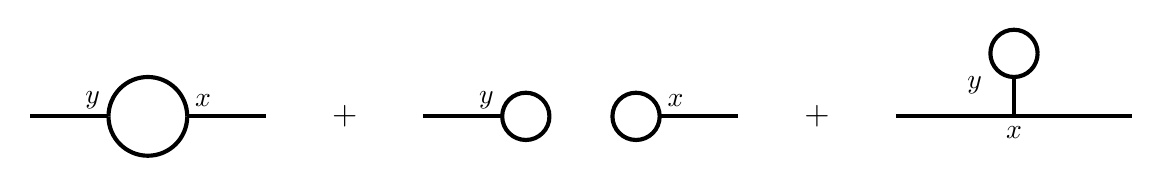
\begin{tikzpicture}[line width=1.5pt]
    % First diagram
    \draw (0:1) -- (0,0);
    \draw (1,0) arc (180:0:0.5);
    \draw (1,0) arc (-180:0:0.5);
    \draw (2,0) -- (3,0);
    \node at (4,0) {\large+};
    \node at (0.8, 0.2) {$y$};
    \node at (2.2, 0.2) {$x$};
    
    % Second diagram
    \draw (5,0) -- (6,0);
    \draw (6.6,0) arc (0:360:0.3);
    \draw (8,0) arc (0:360:0.3);
    \draw (8,0) -- (9,0);
    \node at (10,0) {\large+};
    \node at (5.8, 0.2) {$y$};
    \node at (8.2, 0.2) {$x$};
    
    % Third diagram
    \draw (11,0) -- (12.5,0);
    \draw (12.5,0) -- (12.5,0.5);
    \draw (12.8,0.8) arc (0:360:0.3);
    \draw (12.5,0) -- (14,0);
    \node at (12, 0.4) {$y$};
    \node at (12.5, -0.2) {$x$};
\end{tikzpicture}
\end{center}
These diagrams have new points, labelled $x$ an $y$, which are integrated over.

From these examples, we can infer that the perturbative expansion will also work for higher-order terms or order interactions.


\begin{enumerate}[leftmargin=*]
    \item Start with (external) points \( x_i \) for each position at which fields in the correlation function are evaluated. Draw a line from each point.
    
    \item A line can then either contract to an existing line, giving a Feynman propagator connecting the endpoints of the two lines, or it can split, due to an interaction. A split gives a new (internal) vertex proportional to the coefficient of \( \mathcal{L}_{\text{int}}[\phi] \) times \( i \) and new lines corresponding to the fields in \( \mathcal{L}_{\text{int}}[\phi] \).
    \item At a given order in the perturbative couplings, the result is the sum of all diagrams with all the lines contracted, integrated over the positions of internal vertices.
    \item Drop all $n!$ factors in the coefficient of interactions
\end{enumerate}


These are known as the position-space Feynman rules. The result is a set of diagrams. The original time-ordered product is given by a sum over integrals represented by the diagrams with an appropriate numerical factor. To determine the numerical factor, it is conventional to write interactions normalized by the number of permutations of identical fields, for example

\[
\mathcal{L}_{\text{int}} = \frac{\lambda}{4!} \phi^4, \quad \frac{g}{3!} \phi^3, \quad \frac{\kappa}{5!\,3!\,2!} \phi_1^5 \phi_2^3 \phi_3^2, \ldots
\tag{7.24}
\]

Thus, when the derivative is taken to turn the interaction into a vertex, the prefactor becomes $\frac{1}{(n-1)!}$. This $(n-1)!$ is then cancelled by the number of permutations of the lines coming out of the vertex, not including the line coming in, which we already fixed. In this way, the $n!$ factors all cancel. The diagram is therefore associated with just the prefactor $\lambda$, $g$, $\kappa$, etc. from the interaction.

In some cases, such as theories with real scalar fields, some of the permutations give the same amplitude. For example, if a line connects back to itself, then permuting the two legs gives the same integral. In this case, a factor of $\frac{1}{2}$ in the normalisation is not cancelled, so we must divide by 2 to get the prefactor for a diagram. So there is one more rule:

\begin{enumerate}
\setcounter{enumi}{3}
\item Drop all the $n!$ factors in the coefficient of the interaction, but then divide by the geometrical symmetry factor for each diagram.
\end{enumerate}

Symmetries are ways that a graph can be deformed so that it looks the same with the external points, labelled $x_i$, held fixed.

\subsection{Hamiltonian Derivation}
In this section, we will reproduce the position-space Feynman rules with the Hamiltonian derivation. First, we will start by recalling the Heisenberg picture of quantum mechanics, in which operators must satisfy the equation of motion
\begin{equation}
    i\partial_t\phi(x) = [\phi, H].
\end{equation}
The solution to this equation is
\begin{equation}
    \phi(x) = S^\dagger(t,t_0)\phi(\vec{x})S(t,t_0),
    \label{Eq. Heisenberg}
\end{equation}
where $S(t,t_0)$ is the time-evolution operator ($S$-matrix) that satisfies
\begin{equation}
    i\partial_tS(t,t_0) = H(t)S(t,t_0).
    \label{Eq. Heisenberg 2}
\end{equation}
Also, all states are defined to be time-independent in the Heisenberg picture. Now consider a time-dependent Hamiltonian $H(t)$
\begin{equation}
    H(t) = H_0 + V(t),
\end{equation}
where $H_0$ is called the free Hamiltonian, which can be solved exactly, and $V$ is small compared to $H_0$ in some sense. Also, keep in mind that $\phi(x), H, H_0$ and $V$ are all in Heisenberg picture.

Next, we need to switch to the interaction picture, in which field evolves with $H_0$. The interaction picture scalar fields are just the free fields
\begin{equation}
    \phi_0(x) = e^{iH_0(t-t_0)}\phi(\vec{x})e^{-iH_0(t-t_0)},
\end{equation}
where $\phi(\vec{x})$ is the Schrödinger picture field. Thus, the Schrödinger picture and interaction picture fields are equal at $t = t_0$.

From (\ref{Eq. Heisenberg}), we can see that the interaction picture and the Heisenberg picture are related by
\begin{equation}
\begin{aligned}
        \phi(x) &= S^\dagger(t, t_0)e^{-iH_0(t-t_0)}\phi_0(x)e^{iH_0(t-t_0)}S(t,t_0)\\
        &= U^\dagger(t,t_0)\phi_0(x)U(t,t_0),
        \label{Eq. HD phi define}
\end{aligned}
\end{equation}
where $U(t,t_0) \equiv e^{iH_0(t-t_0)}S(t,t_0)$.

We can obtain a differential equation for $U(t, t_0)$ with (\ref{Eq. Heisenberg 2}):
\begin{equation}
    \begin{aligned}
        i\partial_tU(t,t_0) &= i\partial_t[e^{iH_0(t-t_0)}S(t,t_0)]\\
        &=e^{iH_0(t-t_0)}[-H_0 + i\partial_tS(t,t_0)]\\
        &=e^{iH_0(t-t_0)}[-H_0 + H(t)]S(t,t_0)\\
        &=e^{iH_0(t-t_0)}[-H_0 + H(t)]e^{-iH_0(t-t_0)}e^{iH_0(t-t_0)}S(t,t_0)\\
        &=V_I(t)U(t,t_0),
    \end{aligned}
\end{equation}
where $V_I(t) = e^{iH_0(t-t_0)}V(t)e^{-iH_0(t-t_0)}$ is $V(t)$ in the interaction picture. If everything commuted in this equation, then the solution would simply be $U(t, t_0) = \text{exp}[-i\int^t_{t_0} dt' V_I(t') ]$. However, $V_I(t_1)$ does not necessarily commutes with $V_I(t_2)$, and hence the right solution would be
\begin{shaded}
    \begin{equation}
        U(t, t_0) = T\biggr\{\text{exp}\biggr[-i\int^t_{t_0} dt' V_I(t') \biggr]\biggr\}.
        \label{Eq. U}
    \end{equation}
\end{shaded}

\begin{tcolorbox}[breakable, colback=yellow!20!white, colframe=black, boxrule=1pt]
    (\ref{Eq. U}) can be proven with perturbation theory.

    For simplicity, we will remove the subscript of $V$, and thus
    \begin{equation}
        i\partial_tU(t,t_0)  = V(t)U(t,t_0).
    \end{equation}
    Integrate over $t$ on both sides, we have
    \begin{equation}
        U(t, t_0) = 1 - i\int^t_{t_0} dt' V(t') U(t', t_0),
    \end{equation}
    where we have chosen the boundary condition so that $U(t, t)=1$.

    To $\text{0}^{\text{th}}$ order of $V$, we have
    \begin{equation}
        U(t, t_0) = 1.
    \end{equation}
    To first order in $V$, we find
    \begin{equation}
        U(t, t_0) = 1 - i\int^t_{t_0} dt' V(t') + \cdots.
    \end{equation}
    To second order in $V$, we would obtain
    \begin{equation}
    \begin{aligned}
                U(t, t_0) &= 1 - i\int^t_{t_0} dt' V(t') \biggr[ 1 - i\int^{t'}_{t_0} dt'' V(t'') + \cdots \biggr]\\
                &= 1 - i\int^t_{t_0} dt' V(t') + (-i)^2\int^t_{t_0} dt'\int^{t'}_{t_0} dt''V(t')V(t'') + \cdots.
    \end{aligned}
    \end{equation}
    The second integral has $t_0<t''<t'<t$, thus
    \begin{equation}
        \int^t_{t_0} dt'\int^{t'}_{t_0} dt''V(t')V(t'') = \int^t_{t_0} dt'' \int^{t}_{t''} dt' V(t')V(t'').
    \end{equation}
    Now, by interchanging $t'$ and $t''$, we have
    \begin{equation}
        \int^t_{t_0} dt'\int^{t'}_{t_0} dt''V(t')V(t'') = \int^t_{t_0} dt'\int^{t}_{t'} dt''V(t')V(t'').        
    \end{equation}
    Average these two terms:
    \begin{equation}
        \begin{aligned}
             \int^t_{t_0} dt'\int^{t'}_{t_0} dt''V(t')V(t'') &= \frac{1}{2}  \int^t_{t_0} dt'\biggr[\int^{t'}_{t_0} dt''V(t')V(t'') + \int^{t}_{t'} dt''V(t')V(t'')\biggr]\\
             &= \frac{1}{2}  \int^t_{t_0} dt'\biggr[\int^{t}_{t_0} dt''V(t')V(t'')\theta(t'-t'') + \int^{t}_{t_0} dt''V(t')V(t'')\theta(t'-t'') \biggr]\\
             &= \frac{1}{2}  \int^t_{t_0} dt'\int^{t}_{t_0} dt'' T\{V(t')V(t'')\}.
        \end{aligned}
    \end{equation}
    Thus,
    \begin{equation}
        U(t,t_0) = 1 - i\int^t_{t_0} dt' V(t') + \frac{(-i)^2}{2}  \int^t_{t_0} dt'\int^{t}_{t_0} dt'' T\{V(t')V(t'')\} + \cdots.
    \end{equation}
    And one can prove, by induction, that
    \begin{equation}
        U(t, t_0) = T\biggr\{\text{exp}\biggr[-i\int^t_{t_0} dt' V_I(t')\biggr]\biggr\}.
    \end{equation}
    
\end{tcolorbox}
\subsubsection{$U$ Relations}
It is convenient to write
\begin{equation}
    U_{21} \equiv U(t_2, t_1) = T\biggr\{\text{exp}\biggr[-i\int^{t_2}_{t_1} dt' V_I(t')\biggr]\biggr\}.
\end{equation}
Thus, we have
\begin{equation}
    U_{21}U_{12} = 1,
\end{equation}
\begin{equation}
    U_{21}^{-1} = U_{21}^\dagger = U_{12},
\end{equation}
and for $t_3 > t_2 > t_1$
\begin{equation}
    U_{32}U_{21} = U_{31}.
\end{equation}
Multiplying $U_{12}$ on both sides:
\begin{equation}
    U_{31}U_{12} = U_{32}.
\end{equation}
Finally, from (\ref{Eq. HD phi define}), we can write
\begin{equation}
    \phi(x_1) = U_{10}^\dagger\phi_0(x_1)U_{10} = U_{01}\phi_0(x_1)U_{10}.
\end{equation}

\subsubsection{Vacuum Matrix Elements}
In the LSZ reduction formula, we have used the vacuum state $\ket{\Omega}$, which behaves the same way as the state $\ket{0}$ in the free theory at $t= \pm \infty$. Hence, these two states must be proportional at $t= \pm \infty$. Since the free theory and the interacting theory are equivalent at $t = t_0$, (in the Schrödinger picture) $e^{-iH_0(t-t_0)}\ket{0}$ is proportional to $S(t,t_0)\ket{\Omega}$ at $t = \pm \infty$. Thus
\begin{equation}
    \ket{\Omega} = \mathcal{N}_i\lim_{t\rightarrow-\infty} S(t, t_0)^\dagger e^{-iH_0(t-t_0)}\ket{0} = \mathcal{N}_i U(t,t_0)^\dagger\ket{0} = \mathcal{N}_i U_{0-\infty}\ket{0},
\end{equation}
\begin{equation}
    \bra{\Omega} = \mathcal{N}_f \bra{0}U_{\infty0},
\end{equation}
where $\mathcal{N}_i$ and $\mathcal{N}_f$ are constants to be determined.

We are interested in the time-ordered product $\bra{\Omega}T\{\phi(x_1) \phi(x_2) \cdots  \phi(x_n)\}\ket{\Omega}$. We can assume $t_1 > t_2 > \cdots > t_n$ with no loss of generality. Hence,
\begin{equation}
    \begin{aligned}
        \bra{\Omega}T\{\phi(x_1) \phi(x_2) \cdots  \phi(x_n)\}\ket{\Omega} &= \bra{\Omega}\phi(x_1) \phi(x_2) \cdots  \phi(x_n)\ket{\Omega}\\
        &= \mathcal{N}_i \mathcal{N}_f \bra{0}U_{\infty0}\phi(x_1) \phi(x_2) \cdots  \phi(x_n)U_{0-\infty}\ket{0}\\
        &=  \mathcal{N}_i \mathcal{N}_f \bra{0}U_{\infty0} U_{01} \phi_0(x_1) U_{10} U_{02}\phi_0(x_2) U_{20} \cdots U_{0n} \phi_0(x_n) U_{n0}U_{0-\infty}\ket{0}\\
        &= \mathcal{N}_i \mathcal{N}_f \bra{0}U_{\infty1} \phi_0(x_1) U_{12} \phi_0(x_2) U_{23} \cdots U_{(n-1)n} \phi_0(x_n) U_{n-\infty}\ket{0}\\
        &= \mathcal{N}_i \mathcal{N}_f \bra{0}T\{U_{\infty1} \phi_0(x_1) U_{12} \phi_0(x_2) U_{23} \cdots U_{(n-1)n} \phi_0(x_n) U_{n-\infty}\}\ket{0}\\
        &= \mathcal{N}_i \mathcal{N}_f \bra{0}T\{\phi_0(x_1)\phi_0(x_2) \cdots \phi_0(x_n) U_{\infty-\infty}\}\ket{0},
    \end{aligned}
\end{equation}
where we have put the time-order operator back in, which is legal because everything is in time-order. 

Next, we require the normalisation to be $\braket{\Omega}{\Omega} = 1$. Thus,
\begin{equation}
    \bra{\Omega}T\{\phi(x_1) \phi(x_2) \cdots  \phi(x_n)\}\ket{\Omega} = \frac{\bra{0}T\{\phi_0(x_1)\phi_0(x_2) \cdots \phi_0(x_n) U_{\infty-\infty}\}\ket{0}}{\ \bra{0}U_{\infty-\infty}\ket{0}}.
\end{equation}
Then, 
\begin{equation}
    \bra{\Omega}T\{\phi(x_1) \phi(x_2) \cdots  \phi(x_n)\}\ket{\Omega} = \frac{\bra{0}T\biggr\{\phi_0(x_1)\phi_0(x_2) \cdots \phi_0(x_n) \text{exp}\biggr[-i\int^{\infty}_{-\infty} dt V_I(t)\biggr]\biggr \}\ket{0}}{\ \bra{0}T\biggr \{ \text{exp}\biggr[-i\int^{\infty}_{-\infty} dt V_I(t)\biggr]\biggr\}\ket{0}}.
    \label{Eq. HD 1}
\end{equation}
Now, recall
\begin{equation}
    V_I(t) = \int d^3x \mathcal{H}_{\text{int}}[\phi_0] = -\int d^3x \mathcal{L}_{\text{int}}[\phi_0].
\end{equation}
Here, $\mathcal{H}_{\text{int}}$ and $\mathcal{L}_{\text{int}}$ are functions of $\phi_0$ because we are in the interaction picture (operators only evolves with the free Hamiltonian). Thus, (\ref{Eq. HD 1}) becomes
\begin{shaded}
    \begin{equation}
        \bra{\Omega}T\{\phi(x_1) \phi(x_2) \cdots  \phi(x_n)\}\ket{\Omega} = \frac{\bra{0}T\biggr\{\phi_0(x_1)\phi_0(x_2) \cdots \phi_0(x_n) \text{exp}\biggr[i\int^{\infty}_{-\infty} d^4x \mathcal{L}_{\text{int}}[\phi_0]\biggr]\biggr \}\ket{0}}{\ \bra{0}T\biggr \{ \text{exp}\biggr[i\int^{\infty}_{-\infty} d^4x \mathcal{L}_{\text{int}}[\phi_0]\biggr]\biggr\}\ket{0}}.
        \label{Eq. HD 2}
    \end{equation}
\end{shaded}
Now consider the case, where
\begin{equation}
    \mathcal{L}_{\text{int}}[\phi] = \frac{g}{3!}\phi^3,
\end{equation}
and consider the 2-point correlation function $\bra{0}T\{\phi_0(x_1)\phi_0(x_2)\}\ket{0}$. The numerator of (\ref{Eq. HD 2}) can be expanded perturbatively as
\begin{equation}
    \begin{aligned}
        \bra{0}T\biggr\{\phi_0(x_1)\phi_0(x_2) &\text{exp}\biggr[i\int^{\infty}_{-\infty} d^4x \frac{g}{3!}\phi_0^3\biggr]\biggr \}\ket{0} = \bra{0}T\{\phi_0(x_1)\phi_0(x_2)\}\ket{0}\\
        &+ \frac{ig}{3!}\int d^4x \bra{0}T\{\phi_0(x_1)\phi_0(x_2)\phi_0(x)^3\}\ket{0}\\
        &+ \biggr(\frac{ig}{3!}\biggr)^2\frac{1}{2}\int d^4x \int d^4y \bra{0}T\{\phi_0(x_1)\phi_0(x_2)\phi_0(x)^3\phi_0(y)^3\}\ket{0} + \cdots.
    \label{Eq. HD expansion}
    \end{aligned}
\end{equation}
Hence, the problem we are left with is to evaluate $n$-point correlation function in the free theory.

\subsubsection{Normal ordering and Wick's Theorem}
The key to computing an $n$-point correlation function is to develop the Wick's theorem. First, we will write $\phi_0(x)$ as
\begin{equation}
    \phi_0(x) = \phi_0^+(x) + \phi_0^-(x),
\end{equation}
where
\begin{equation}
    \phi_0^+(x) \equiv \int \frac{d^3p}{(2\pi)^3} \frac{1}{2\omega_p} a_p e^{-ipx}, \quad \phi_0^-(x) \equiv \int \frac{d^3p}{(2\pi)^3} \frac{1}{2\omega_p} a_p^\dagger e^{ipx}.
\end{equation}
Now, consider $T\{\phi_0(x)\phi_0(y)\}$ with $x^0 > y^0$:
\begin{equation}
\begin{aligned}
    &T\{\phi_0(x)\phi_0(y)\}\\
    &= \phi_0^+(x)\phi_0^+(y) + \phi_0^+(x)\phi_0^-(y) + \phi_0^-(x)\phi_0^+(y) + \phi_0^-(x)\phi_0^-(y)\\
    &= \phi_0^+(x)\phi_0^+(y) + \phi_0^-(y)\phi_0^+(x) + \phi_0^-(x)\phi_0^+(y) + \phi_0^-(x)\phi_0^-(y) + [\phi_0^+(x), \phi_0^-(y)].
    \label{Eq. Wick 1}
\end{aligned}
\end{equation}
Note, here all the annihilation operators $a$ are on the right except for the commutator. However, the commutator would generate a number, so the order does not matter. Such an expression is said to be normal ordered.

Let us define a normal ordering operation, $:a_pa_q a_k^\dagger\ldots:$, such that place whatever operators it contains in normal order. For example,
\begin{shaded}
    \begin{equation}
        :a_pa_ka_q^\dagger: = a_q^\dagger a_pa_k.
    \end{equation}
\end{shaded}
Hence, (\ref{Eq. Wick 1}) becomes
\begin{equation}
    T\{\phi_0(x)\phi_0(y)\} = :\phi_0(x)\phi_0(y) + [\phi_0^+(x), \phi_0^-(y)]:, \qquad \qquad (x^0 > y^0).
\end{equation}
Similarly, for $x^0 < y^0$, we have
\begin{equation}
    \bra{0}T\{\phi_0(x)\phi_0(y)\}\ket{0} = :\phi_0(x)\phi_0(y) + [\phi_0^+(y), \phi_0^-(x)]:, \qquad \qquad (x^0 < y^0).
\end{equation}
Therefore, let us define another quantity called contraction of two fields, which is 
\begin{shaded}
    \begin{equation}
    \begin{aligned}
    \wick{\c\phi(x)\c\phi(y)} \equiv 
    \begin{cases} 
        \big[\phi^+(x), \phi^-(y)\big] & \text{for } x^0 > y^0; \\ 
        \big[\phi^+(y), \phi^-(x)\big] & \text{for } y^0 > x^0,
    \end{cases}
\end{aligned}
\end{equation}
\end{shaded}
where we have made the subscript implicit, as contractions always involves interaction picture operators.
Thus,
\begin{equation}
        T\{\phi_0(x)\phi_0(y)\} = :\phi_0(x)\phi_0(y) + \wick{\c\phi_0(x) \c\phi_0(y)}.
\end{equation}
Generally,
\begin{shaded}
    \begin{equation}
        T\{\phi_0(x_1)\phi_0(x_2) \cdots \phi_0(x_n)\} = :\phi_0(x_1)\phi_0(x_2) \cdots \phi_0(x_n)\ + (\text{all possible contractions}):.
    \end{equation}
\end{shaded}
This is known as the Wick's theorem, which can be proven by induction. We have already shown it is true with $m=2$ fields. Now, let us prove: if this is true for $m=n$ fields, then it must also be true for $m=n+1$ fields. We will assume $x_1^0 > x_2^0 > \cdots > x_{n+1}^0$.
\begin{equation}
    \begin{aligned}
        T\{\phi_1\phi_2 \dots \phi_{n+1}\}= :\phi_1\phi_2 \cdots \phi_n + (\text{all possible contractions without $\phi_{n+1}$}):(\phi^+_{n+1} + \phi^-_{n+1}).
    \end{aligned}
\end{equation}
Then,
\begin{equation}
\begin{aligned}
        &:\phi_1\phi_2 \cdots \phi_n:\phi^-_{n+1} \\
        &= :(\phi_1^+ + \phi_1^-)(\phi_2^+ + \phi_2^-) \cdots (\phi_n^+ + \phi_n^-):\phi^-_{n+1}\\
        &= (\phi_1^+\phi_2^+ \dots \phi_n^+ + \phi_1^-\phi_2^+ \dots \phi_n^+ +
        \phi_2^-\phi_1^+\phi_3^+ \dots \phi_n^+ + \cdots + \phi_1^-\phi_2^- \dots \phi_n^-)\phi^-_{n+1}\\
        &= :\phi^-_{n+1}\phi_1\phi_2 \cdots \phi_n: + (\text{all possible contractions involving $\phi_{n+1}$}).
\end{aligned} 
\end{equation}
Hence, we have proven the Wick's theorem.

\subsubsection{Position-Space Feynman Rules Revisited}
With Wick's theorem, we can now evaluate the $n$-point correlation function:
\begin{equation}
\begin{aligned}
        \bra{0}T\{\phi(x_1)\phi(x_2) \cdots \phi(x_n)\}\ket{0} &= \bra{0}:\phi_0(x_1)\phi_0(x_2) \cdots \phi_0(x_n)\ + (\text{all possible contractions}):\ket{0}\\
        &= \sum(\text{all possible contractions which all $\phi_i$ is involved}),
        \label{Eq. HD contract}
\end{aligned}
\end{equation}
where we have used the fact that $\bra{0}:\cdots:\ket{0} = 0$ as long as there is any operator in the normal ordering operator.

Each contraction represents the creation and annihilation of a particle, with the the creation happening earlier than the annihilation. In particular,
\begin{equation}
\begin{aligned}
        \wick{\c\phi(x)\c\phi(y)}=\bra{0}\wick{\c\phi(x)\c\phi(y)}\ket{0}&=
        \begin{cases} 
        \bra{0}\big[\phi^+(x), \phi^-(y)\big]\ket{0} & \text{for } x^0 > y^0; \\ 
        \bra{0}\big[\phi^+(y), \phi^-(x)\big]\ket{0} & \text{for } y^0 > x^0,
    \end{cases}
    \\
    &=
    \begin{cases}
        \bra{0}\phi^+(x)\phi^-(y)\ket{0} & \text{for } x^0 > y^0; \\ 
        \bra{0}\phi^+(y)\phi^-(x)\ket{0} & \text{for } y^0 > x^0,
    \end{cases}
\end{aligned}
\end{equation}
which is exactly the part contributing to the Feynman propagator. Hence, we can conclude that
\begin{equation}
    \wick{\c\phi(x)\c\phi(y)} = D_F(x, y) = \int \frac{d^4q }{(2\pi)^4} \frac{i}{q^2 - m^2 +i\epsilon} e^{iq(x-y)}.
\end{equation}

Then, we can apply (\ref{Eq. HD contract}) to (\ref{Eq. HD expansion}). The second term of (\ref{Eq. HD expansion}) gives zero, since there is an odd number of fields, which means there will always be an extra $\phi$ left outside the contractions annihilating the state $\ket{0}$.

The third term of (\ref{Eq. HD expansion}) involves eight fields, and there are multiple possible contractions:
\begin{equation}
    \begin{aligned}
        &\bra{0}T\{\phi_0(x_1)\phi_0(x_2)\phi_0(x)\phi_0(x)\phi_0(x)\phi_0(y)\phi_0(y)\phi_0(y)\}\ket{0}.
    \end{aligned}
\end{equation}
For example, one possible contraction would be
\begin{equation}
    \wick{\c1 \phi_0(x_1)\c2 \phi_0(x_2)\c1 \phi_0(x)\c3 \phi_0(x)\c4 \phi_0(x)\c2 \phi_0(y)\c3 \phi_0(y)\c4 \phi_0(y)} = D_{1x}D_{2y}D_{xy}^2.
\end{equation}
There are
\begin{equation}
    3 \times 3 \times 2 = 9
\end{equation}
numbers of permutations of this contraction. Including these permutation factors, (\ref{Eq. HD expansion}) to second order of $g$ becomes
\begin{equation}
    \begin{aligned}
        \bra{\Omega} T \{ \phi(x_1) \phi(x_2) \} \ket{\Omega} 
&= \frac{1}{\bra{0} T \{ e^{i \int \mathcal{L}_{\text{int}} }\}  \ket{0}} 
\bigg\{ D_{12} \\
&\quad - g^2 \int d^4x \int d^4y \bigg[ 
\frac{1}{8} D_{12} D_{xx} D_{xy} D_{yy} + \frac{1}{12} D_{12} D_{xy}^3 \\
&\quad + \frac{1}{2} D_{1x} D_{2x} D_{xy} D_{yy} + \frac{1}{4} D_{1x} D_{xx} D_{yy} D_{y2} \\
&\quad + \frac{1}{2} D_{1x} D_{xy}^2 D_{y2} \bigg] + \cdots \bigg\}.
    \end{aligned}
\end{equation}
Comparing to (\ref{Eq. PF expansion}), we note that they are identical, except the first second terms in the integration and the extra $\bra{0} T \{ e^{i \int \mathcal{L}_{\text{int}} }\}\ket{0}$ factor. The two new terms correspond to the diagrams
\begin{center}
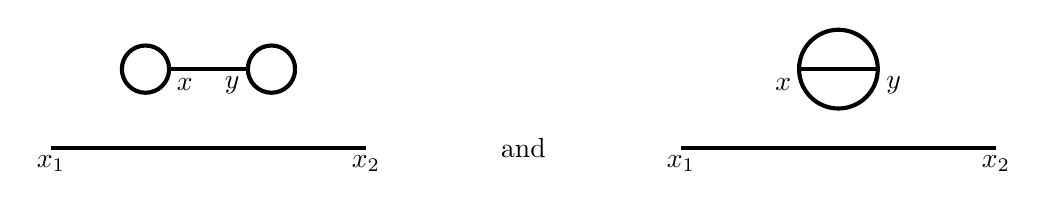
\begin{tikzpicture}[line width=1.5pt]
    \draw (0,0) -- (4,0);
    \draw (1.5,1) -- (2.5,1);
    \draw (1.5,1) arc (360:0:0.3);
    \draw (3.1,1) arc (360:0:0.3);
    \node at (1.7, 0.8) {$x$};
    \node at (2.3, 0.8) {$y$};
    \node at (0,-0.2) {$x_1$};
    \node at (4,-0.2) {$x_2$};

    \node at (6,0) {and};

    \draw (8,0) -- (12,0);
    \draw (9.5,1) -- (10.5,1);
    \draw (9.5,1) arc (180:0:0.5);
    \draw (9.5,1) arc (-180:0:0.5);
    \node at (9.3, 0.8) {$x$};
    \node at (10.7, 0.8) {$y$};
    \node at (8,-0.2) {$x_1$};
    \node at (12,-0.2) {$x_2$};
    
\end{tikzpicture}
\end{center}
Note that these two diagrams both have bubbles, which are connected subgraphs not including any external points. Hopefully, the $\bra{0} T \{ e^{i \int \mathcal{L}_{\text{int}} }\}\ket{0}$ factor would cancel the bubbles exactly, so that we can recover position-space Feynman rules with the Hamiltonian approach. Let us try expanding the denominator in (\ref{Eq. HD expansion}) up to order of $g^2$, we have
\begin{equation}
\begin{aligned}
        \bra{0} T \{ e^{i \int \mathcal{L}_{\text{int}} }\}\ket{0} &= 1 + \biggr(\frac{ig}{3!}\biggr)^2 \frac{1}{2} \int d^4x \int d^4y \bra{0}T\{\phi_0(x)^3 \phi_0(y)^3\} \ket{0} + \mathcal{O}(g^4) \\
        &= 1 + \biggr(\frac{ig}{3!}\biggr)^2 \frac{1}{2} \int d^4x \int d^4y  [9D_{xx} D_{xy} D_{yy} + 6D_{xy}^3] + \mathcal{O}(g^4)\\
        &= 1 -g^2 \int d^4x \int d^4y  [\frac{1}{8}D_{xx} D_{xy} D_{yy} + \frac{1}{12}D_{xy}^3] + \mathcal{O}(g^4)
\end{aligned}
\end{equation}

Thus, including terms up to second order of $g$ in the denominator and numerator, we have
\begin{equation}
    \bra{\Omega} T \{ \phi(x_1) \phi(x_2) \} \ket{\Omega} = \frac{D_{12}-g^2 \int  [\frac{1}{8}D_{12}D_{xx} D_{xy} D_{yy} + \frac{1}{12}D_{12}D_{xy}^3 + \cdots] + \mathcal{O}(g^4)}{1 -g^2 \int  [\frac{1}{8}D_{xx} D_{xy} D_{yy} + \frac{1}{12}D_{xy}^3] + \mathcal{O}(g^4)}.
\end{equation}
 In perturbation theory, $\frac{1}{1+g^2x+\mathcal{O}(g^4)} =1-g^2x+\mathcal{O}(g^4)$, and hence the bubbles are cancelled exactly. 

 More generally, the bubbles will always cancel. Since the integrals in the expansion of the numerator corresponding to the bubbles never involve any external point, they just factor out. The sum over all graphs, in the numerator, is then the sum over all graphs with no bubbles multiplying the sum over the bubbles. The sum over bubbles is exactly $ \bra{0} T \{ e^{i \int \mathcal{L}_{\text{int}} }\}\ket{0}$. So,
\begin{equation}
    \bra{\Omega}T\{\phi(x_1)\phi(x_2)\}\ket{0} =  \bra{0} T \{\phi_0(x_1)\phi_0(x_2) e^{i \int \mathcal{L}_{\text{int}} }\}\ket{0}_{\text{no bubbles}}.
\end{equation}

We have arrived at the same graphs and same factors with both derivations, and thus we have reproduced the position-space Feynman rules (to some extend).

\subsection{Momentum-Space Feynman Rules}
Now, we will see how time-ordered products are simplified, when all the phase-space integrals over the propagators are performed.

Consider the diagram
\begin{center}
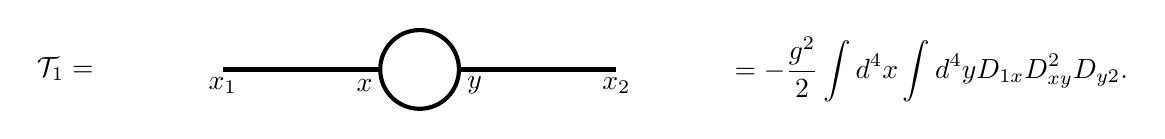
\begin{tikzpicture}[line width=1.5pt]
    \node at (-2,0) {$\displaystyle\mathcal{T}_1=$};
    
    \draw (0,0) -- (2,0);
    \draw (3,0) -- (5,0);
    \draw (3,0) arc (-360:0:0.5);
    \node at (1.8, -0.2) {$x$};
    \node at (3.2, -0.2) {$y$};
    \node at (0,-0.2) {$x_1$};
    \node at (5,-0.2) {$x_2$};

    \node at (9,0) {$\displaystyle=-\frac{g^2}{2}\int d^4x \int d^4y D_{1x}D_{xy}^2D_{y2}.$};
\end{tikzpicture}
\end{center}
First, recall a propagator $D_{xy}$ is given by (take $m=0$ for simplicity)
\begin{equation}
    D_{xy} = \int \frac{d^4p}{(2\pi)^4} \frac{i}{p^2+i\epsilon}e^{ip(x-y)}.
\end{equation}
Hence,
\begin{equation}
\begin{aligned}
        \mathcal{T}_1 = -\frac{g^2}{2} \int d^4x \int d^4y &\int \frac{d^4p_1}{(2\pi)^4}\int \frac{d^4p_2}{(2\pi)^4}\int \frac{d^4p_3}{(2\pi)^4}\int \frac{d^4p_4}{(2\pi)^4} \\
        &\times \frac{i}{p_1^2+i\epsilon}\frac{i}{p_2^2+i\epsilon}\frac{i}{p_3^2+i\epsilon}\frac{i}{p_4^2+i\epsilon} e^{ip_1(x_1-x)}e^{ip_2(y-x_2)}e^{ip_3(x-y)}e^{ip_4(x-y)}.
\end{aligned}
\end{equation}
We can integrate over $x$ and $y$ to get $\delta^4(p_3+p_4-p_1)$ and $\delta^4(p_2-p_3-p_4)$. Thus
\begin{equation}
    \begin{aligned}
        \mathcal{T}_1 &= -\frac{g^2}{2} \int \frac{d^4p_1}{(2\pi)^4}\int \frac{d^4p_2}{(2\pi)^4}\int d^4p_3\int d^4p_4 \\
        &\qquad \qquad \times \frac{i}{p_1^2+i\epsilon}\frac{i}{p_2^2+i\epsilon}\frac{i}{p_3^2+i\epsilon}\frac{i}{p_4^2+i\epsilon} \delta^4(p_3+p_4-p_1) \delta^4(p_2-p_3-p_4) e^{ip_1x_1}e^{-ip_2x_2}\\
        &= -\frac{g^2}{2} \int \frac{d^4p_1}{(2\pi)^4}\int \frac{d^4p_2}{(2\pi)^4}\int d^4p_4\frac{i}{p_1^2+i\epsilon}\frac{i}{p_2^2+i\epsilon}\frac{i}{(p_1-p_4)^2+i\epsilon}\frac{i} {p_4^2+i\epsilon}\delta^4(p_2-p_1) e^{ip_1x_1}e^{-ip_2x_2}\\
    \end{aligned}
\end{equation}
Next, we plug this back into the LSZ reduction formula to get

\begin{equation}
\begin{aligned}
        \bra{f}S\ket{i} &= \biggr[ -i\int d^4x_1e^{-ip_ix_1}(p_i^2) \biggr]\biggr[ -i\int d^4x_2 e^{ip_fx_2}(p_f^2) \biggr] \bra{\Omega}T\{\phi(x_1)\phi(x_2)\}\ket{\Omega}\\
        &= \frac{g^2}{2}\int d^4x_1 \int d^4x_2 \int \frac{d^4p_1}{(2\pi)^4}\int \frac{d^4p_2}{(2\pi)^4}\int d^4p_4 \\
        &\qquad \qquad \times p_i^2 p_f^2\frac{i}{p_1^2+i\epsilon}\frac{i}{p_2^2+i\epsilon}\frac{i}{(p_1-p_4)^2+i\epsilon}\frac{i} {p_4^2+i\epsilon}\delta^4(p_2-p_1) e^{i(p_1-p_i)x_1}e^{-i(p_2-p_f)x_2} + \cdots\\
        &= \frac{g^2}{2}\int d^4p_1\int d^4p_2\int d^4p_4 \\
        &\qquad \qquad \times p_i^2 p_f^2\frac{i}{p_1^2+i\epsilon}\frac{i}{p_2^2+i\epsilon}\frac{i}{(p_1-p_4)^2+i\epsilon}\frac{i} {p_4^2+i\epsilon}\delta^4(p_2-p_1) \delta^4(p_1-p_i) \delta^4(p_2-p_f) + \cdots\\
        &= \frac{g^2}{2} \int d^4p_4 \cancel{p_i^2 p_f^2}\cancel{\frac{i}{p_i^2+i\epsilon}}\cancel{\frac{i}{p_f^2+i\epsilon}}\frac{i}{(p_i-p_4)^2+i\epsilon}\frac{i} {p_4^2+i\epsilon}\delta^4(p_f-p_i) + \cdots\\
        &= \frac{g^2}{2} \int d^4k\frac{i}{(p_i-k)^2+i\epsilon}\frac{i} {k^2+i\epsilon}\delta^4(p_f-p_i) + \cdots,
\end{aligned}
\end{equation}
where we have relabelled $p_4$ as $k$ in the last line. Also, note how the two propagator factors in the beginning get cancelled. This always happens for external legs - remember the point of LSZ was to force the external lines to be on-shell one-particle states.

Recall
\begin{equation}
    S = \mathds{1} + (2\pi)^4\delta^4(\Sigma p_i)i\mathcal{M},
\end{equation}
where $\delta^4(\Sigma p_i)$ in this case is just $\delta^4(p_f-p_i)$. Therefore, we have
\begin{equation}
    i\mathcal{M} = \frac{g^2}{2} \int \frac{d^4k}{(2\pi)^4} \frac{i}{(p_i-k)^2+i\epsilon}\frac{i} {k^2+i\epsilon} + \cdots.
\end{equation}
From this, we can summarise the momentum-space Feynman rules:
\begin{shaded}
\begin{enumerate}
    \item Internal lines (those not connected to external points) get propagators $\frac{i}{p^2-m^2+i\epsilon}$.
    \item Vertices come from interactions in the Lagrangian. They get factors of the coupling constant times $i$. 
    \item Lines connected to external points do not get propagators (their propagators are cancelled by terms from the LSZ reduction formula). 
    \item Momentum is conserved at each vertex.
    \item Integrate over undetermined 4-momenta. 
    \item Sum over all possible diagrams.
\end{enumerate}
\end{shaded}

\subsubsection{Disconnected Graphs}
\begin{center}
\begin{tikzpicture}[baseline=(current bounding box.center)]
  \begin{feynman}
    \vertex (a);
    \vertex [right=of a] (b);
    \vertex [above right=of b] (f1);
    \vertex [below right=of b] (c);
    \vertex [above right=of c] (f2);
    \vertex [below right=of c] (f3);
    \vertex [above= of a] (a1);
    \vertex [above= of a1] (a2);
    \vertex [right=of a2] (b2);
    \vertex [below right=of b2] (f12);
    \vertex [above right=of b2] (c2);
    \vertex [below right=of c2] (f22);
    \vertex [above right=of c2] (f32);
    \vertex [left= of a] (a0);
    \vertex [left= of a2] (a02);

    \diagram* {
      (a0) --[fermion] (a) -- (b) -- [fermion] (f1),
      (b) -- [boson] (c),
      (c) -- [anti fermion] (f2),
      (c) -- [fermion] (f3),
      (a02) --[fermion] (a2) -- (b2) -- [fermion] (f12),
      (b2) -- [boson] (c2),
      (c2) -- [anti fermion] (f22),
      (c2) -- [fermion] (f32),
    };
  \end{feynman}
  \node[below] at (current bounding box.south) {Diagram 1};
\end{tikzpicture}
\hspace{1cm} % 添加水平间距
\begin{tikzpicture}[baseline=(current bounding box.center)]
  \begin{feynman}
    \vertex (a);
    \vertex [right=of a] (b);
    \vertex [above right=of b] (f1);
    \vertex [below right=of b] (c);
    \vertex [above right=of c] (f2);
    \vertex [below right=of c] (f3);
    \vertex [above= of a] (a1);
    \vertex [above= of a1] (a2);
    \vertex [right=of a2] (b2);
    \vertex [below right=of b2] (f12);
    \vertex [above right=of b2] (c2);
    \vertex [below right=of c2] (f22);
    \vertex [above right=of c2] (f32);
    \vertex [left= of a] (a0);
    \vertex [left= of a2] (a02);

    \diagram* {
      (a0) --[fermion] (a) -- (b) -- [fermion] (f1),
      (b) -- [boson] (c),
      (c) -- [anti fermion] (f2),
      (c) -- [fermion] (f3),
      (a02) --[fermion] (a2) -- (b2) -- [fermion] (f12),
      (b2) -- [boson] (c2),
      (c2) -- [anti fermion] (f22),
      (c2) -- [fermion] (f32),
      (a) -- [boson] (a2),
    };
  \end{feynman}
  \node[below] at (current bounding box.south) {Diagram 2};
\end{tikzpicture}
\end{center}
A lot of contractions will result in diagrams where some subset of external vertices connect to each other without interacting with the other subsets. How do we handle these graphs where subsets are independently connected?

Consider an 8-point function shown in Diagram 1. Clearly, it contains two separated $1\rightarrow3$ scat-tering. The probability of the total $2\rightarrow6$ scattering is given by the product of the two $1\rightarrow3$ probabilities. Meanwhile, Diagram 2 describes the case where the two subdiagrams do interact.

So, what if there could be interference between the two diagrams? However, this cannot be true. To see why, recall the definition of the matrix element that these time-ordered calculations produce has only a single $\delta$-function:
\begin{equation}
    S = \mathds{1} + i\delta^4(\Sigma p)\mathcal{M}.
\end{equation}
Disconnected matrix elements would have an extra $\delta$-function $\mathcal{M}_\text{disconnected} = \delta^4(\Sigma_\text{subset}p)(\cdots)$. However, connected matrix elements are just integrals over propagators, as given by the Feynman rules. Such integrals can only produce poles or possibly branch cuts, which are never as strong as the singularity produced by the $\delta$-function. Therefore, the disconnected amplitudes are always infinitely larger than the connected ones, and thus the interference vanishes. 

The fact that there can never be more than a single delta function coming from a connected diagram is called cluster decomposition, which is sometimes considered as an axiom of quantum field theory. The cluster decomposition says that experiments well-separated in space cannot influence each other (the connected $S$-matrix should vanish). Constructing local theories out of fields made from creation and annihilation operators guarantees cluster decomposition. However, we do not know if the logic is invertible, that is, if the only possible theories that satisfy cluster decomposition are local field theories constructed out of creation and annihilation operators.

\subsubsection{Mandelstam Variables}
There are three very common diagrams in $2 \rightarrow 2$ scattering. 

\begin{center}
    % s-channel
    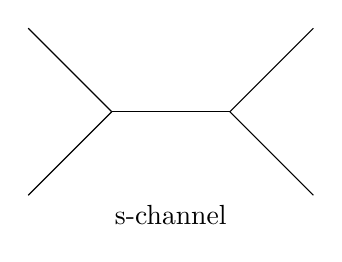
\begin{tikzpicture}[baseline=(current bounding box.center)]
        \begin{feynman}
            \vertex (i1);
            \vertex [below right= of i1] (a);
            \vertex[below left= of a] (i2);
            \vertex [right= of a] (b);
            \vertex [below right= of b] (f2);
            \vertex [above right= of b] (f1);

            \diagram* {
            (i1) -- (a),
            (i2) -- (a),
            (b) -- (a),
            (f1) -- (b),
            (f2) -- (b),
            };
        \end{feynman}
        \node[below] at (current bounding box.south) {s-channel};
    \end{tikzpicture}
    \hspace{1cm}
    % t-channel
    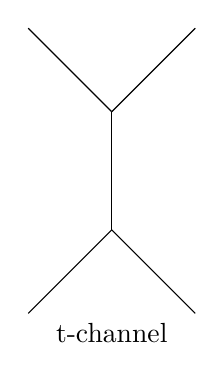
\begin{tikzpicture}[baseline=(current bounding box.center)]
        \begin{feynman}
            \vertex (i1);
            \vertex [below right= of i1] (a);
            \vertex [below= of a] (b);
            \vertex[below left= of b] (i2);
            \vertex [above right= of a] (f1);
            \vertex [below right= of b] (f2);

            \diagram* {
            (i1) -- (a),
            (i2) -- (b),
            (b) -- (a),
            (f1) -- (a),
            (f2) -- (b),
            };
        \end{feynman}
        \node[below] at (current bounding box.south) {t-channel};
    \end{tikzpicture}
    \hspace{1cm}
    % u-channel
    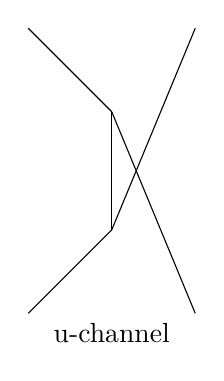
\begin{tikzpicture}[baseline=(current bounding box.center)]
        \begin{feynman}
            \vertex (i1);
            \vertex [below right= of i1] (a);
            \vertex [below= of a] (b);
            \vertex[below left= of b] (i2);
            \vertex [above right= of a] (f1);
            \vertex [below right= of b] (f2);

            \diagram* {
            (i1) -- (a),
            (i2) -- (b),
            (b) -- (a),
            (f1) -- (b),
            (f2) -- (a),
            };
        \end{feynman}
        \node[below] at (current bounding box.south) {u-channel};
    \end{tikzpicture}
\end{center}

These three diagrams are called the s-,u- and t- channel, respectively. Calculation of these diagrams can be simplified by introducing
\begin{equation}
    \begin{aligned}
        s \equiv (p_1+p_2)^2 = (p_3+p_4)^2,\\
        t \equiv (p_1-p_3)^2 = (p_2-p_4)^2,\\
        u \equiv (p_1-p_4)^2 = (p_2-p_3)^2.
    \end{aligned}
\end{equation}
These satisfy
\begin{equation}
    s + u + t = \sum m_j,
\end{equation}
where $m_j$ are the invariant masses of particles. These variables correspond to the momentum in the propagator, $p_\mu^2 = s, t$ or $u$, which is Lorentz-invariant.

It turns out that $s$, $t$ and $u$ simplify calculations in many scenarios. As these variables are Lorentz-invariant, we can compute $\mathcal{M}(s,t,u)$ in centre of mass frame, and then we can easily transform into other frames.

\subsubsection{Derivative Couplings}
Suppose we have an interaction involving derivatives, such as
\begin{equation}
    \mathcal{L}_\text{int} = \lambda \phi_1 (\partial_\mu\phi_2)(\partial_
\mu\phi_3).
\end{equation}
In momentum space, these derivatives simply give factors of $ip_\mu$ when a particle is created, and $-ip_\mu$ when a particle is annihilated. Therefore, we get a minus sign for incoming momentum and a plus sign for outgoing momentum.

\subsubsection{Total Derivatives}
We would also like to show that total derivatives does not contribute to the matrix element. Suppose we have
\begin{equation}
    \mathcal{L}_\text{int} = \partial_\mu(\phi_1\cdots\phi_n).
\end{equation}
Suppose each vertex would have given $V$ without the derivatives, adding the derivatives gives
\begin{equation}
    -i(\sum_\text{incoming} p^i_\mu - \sum_\text{outgoing}p^j_\mu) V.
\end{equation}
From Feynman rules, we know that the sum of incoming momenta is equal to the sum of outgoing momenta, and thus the above vanishes. Hence, we can conclude that total derivative does not contribute to the matrix elements.


{\LARGE \bf Quantum Electrodynamic}
\section{Spin 1 and Gauge Invariance}
\subsection{Unitary Representation of Poincaré Group}
The group of translations and Lorentz transformations is called the Poincaré group, ISO(1,3) (the isometry group of Minkowski space).

Our universe is filled with all different kinds of particles. Particles have mass and spin and all kinds of different quantum numbers. They also have values such as momentum and spin projection. If we perform a rotation or a boost, the momentum and spin projection would change, but the quantum numbers would not change. So a particle can be defined as a set of states that only mix with each other under the Poincaré transformations. We can write
\begin{equation}
    \ket{\psi}\rightarrow \mathcal{P}\ket{\psi},
\end{equation}
where $\mathcal{P}$ represents the Poincaré transformation. A set of objects $\psi$ that mix under a transformation is called a representation of the group. Generally, in a given representation there should be a basis for the states $\ket{\psi}$, call it $\{\ket{\psi_i}\}$, where $i$ can be either a discrete or a continuous index, so that
\begin{equation}
    \ket{\psi}\rightarrow \mathcal{P}_i\ket{\psi_{ij}},
\end{equation}
where the transformed states are expressible in the original basis. If there are no subsets of states that transform only among themselves, the representation is irreducible.

We are interested in matrix elements in field theory, which is given by 
\begin{equation}
    \mathcal{M} = \braket{\psi_1}{\psi_2}.
\end{equation}
Under a Poincaré transformation, $\mathcal{M}$ transforms as 
\begin{equation}
    \mathcal{M} =  \braket{\psi_1}{\psi_2} \rightarrow  \bra{\psi_1}\mathcal{P}^\dagger\mathcal{P}\ket{\psi_2}.
\end{equation}
As matrix elements should be Poincaré invariant, we require $\mathcal{P}$ to be unitary, $\mathcal{P}^\dagger\mathcal{P} = 1$. The unitary representations of the Poincaré are only a small subset of all the representations of the Poincaré group. However, we can only compute the matrix elements with the unitary ones. Therefore, we need to know how to find them. Thus,
\begin{shaded}
    \begin{center}
        Particles transform under irreducible unitary representations of the Poincaré group.
    \end{center}
\end{shaded}
This statement is sometimes seen as the definition of particles. 

We have already seen some representations of the Poincaré group, such as the constant tensors, $\phi, V_\mu, T_{\mu\nu}, \ldots$. These are finite-dimensional representations. However, they are not unitary representations. In fact, there are no finite-dimensional representations of the Poincaré group.

The unitary irreducible representations of the Poincaré group were classified by Eugene Wigner in 1939. Wigner showed that irreducible unitary representations are uniquely classified by mass $m$ and spin $J$, where $m$ is a non-negative real number and $J$ is a non-negative half-integer. In addition, Wigner showed that, if $J>0$, for each value of the momentum with $p^2=m^2$ there are $2J+1$ independent states in the representation if $m>0$, and exactly 2 states for $m=0$.

Now, we want to know how to construct a unitary interacting theory of particles in these representations. Thus, we would like to embed the irreducible representations into objects with space-time indices. In particular, we wish to squeeze states of spin 0, ${\frac{1}{2}}$, 1, $\frac{3}{2}$, \ldots into $\phi(x), V_\mu(x), T_{\mu\nu}(x),\ldots$. In this way, we can write out a neat and simple Lagrangian and develop a general way of computing them.

\subsubsection{Unitarity Versus Lorentz Invariance}
It is simple to see the conflict between unitarity and Lorentz invariance. In non-relativistic quantum mechanics, we can have a state, which is a linear combination of spin up $\ket{\uparrow}$ and spin down $\ket{\downarrow}$,
\begin{equation}
    \ket{\psi} = c_1 \ket{\uparrow} + c_2 \ket{\downarrow}.
\end{equation}
Such a state has a norm
\begin{equation}
    \braket{\psi}{\psi} = \abs{c_1}^2 + \abs{c_2}^2 > 0.
\end{equation}

The norm is invariant under rotations, which send
\begin{equation}
    \ket{\uparrow} \rightarrow \cos\theta\ket{\uparrow} + \sin\theta\ket{\downarrow}, \qquad
    \ket{\downarrow} \rightarrow -\sin\theta\ket{\uparrow} + \cos\theta\ket{\downarrow}.
\end{equation}
(The norm is invariant under the larger group SU(2).)

If we want to do the same thing with a basis of four states $\ket{V_\mu}$ which transform as a 4-vector, an arbitrary linear combination would be\
\begin{equation}
    \ket{\psi} = c_0\ket{V_0} + c_1\ket{V_1} + c_2\ket{V_2} + c_3\ket{V_3}.
\end{equation}

Then, the norm would be
\begin{equation}
    \braket{\psi}{\psi} = \abs{c_0}^2 + \abs{c_1}^2 +  \abs{c_2}^2 + \abs{c_3}^2 > 0.
\end{equation}
However, the norm is not Lorentz invariant.

It is natural to modify the norm as
\begin{equation}
     \braket{\psi}{\psi} = \abs{c_0}^2 - \abs{c_1}^2 -  \abs{c_2}^2 - \abs{c_3}^2,
\end{equation}
which is indeed Lorentz invariant. However, it is no longer positive definite. 

In quantum mechanics, we interpret the norm as probability, which needs to be bounded. Suppose we have a positive norm, $\braket{a}{a}$, and a negative norm, $\braket{b}{b}$:
\begin{equation}
    \braket{a}{a} = \abs{a}^2, \quad
    \braket{b}{b} = -\abs{b}^2, \quad
    \braket{b}{a} = c, \quad
    \braket{a}{b} = c^*.
\end{equation}
Applying Gram-Schmidt orthonormalization, we have
\begin{equation}
    \ket{-} = \frac{1}{\abs{b}}\ket{b}, \qquad \ket{+} = \frac{1}{\sqrt{\abs{a}^2 - 3\abs{c/b}^2}}\big(\ket{a} - \frac{c}{\abs{b}^2}\ket{b}\big),
\end{equation}
so that
\begin{equation}
    \braket{+}{+} = 1, \quad
    \braket{-}{-} = -1, \quad
    \braket{+}{-} =  \braket{-}{+} =0.
\end{equation}
A linear combination of $\ket{+}$ and $\ket{-}$ would be
\begin{equation}
    \ket{\psi} = c_+\ket{+} + c_-\ket{-}
\end{equation}
with a norm
\begin{equation}
    \braket{\psi}{\psi} = \abs{c_+}^2 - \abs{c_-}^2.
\end{equation}
Assume $\ket{\psi}$ is normalise, so that $\abs{\braket{\psi}{\psi}}^2 = 1$. Thus, 
\begin{equation}
    \abs{c_+}^2 - \abs{c_-}^2 = \pm 1.
\end{equation}
To have a probability interpretation, we require the probability of observing a certain state to be greater than 0 and smaller than 1. Thus, 
\begin{equation}
    \abs{\braket{+}{\psi}}^2 = \abs{c_+}^2 \quad \text{and} \quad \abs{\braket{-}{\psi}}^2 = \abs{c_-}^2 \implies 0 \leq \abs{c_+}^2, \abs{c_-}^2 \leq 1.
\end{equation}
If $\abs{c_+}^2 = 1 + \abs{c_-}^2$, then $\abs{c_-}^2$ must vanish. Thus, we are only left with the positive norm. Similarly, for $\abs{c_+}^2 = -1 + \abs{c_-}^2$, we are only left with negative norm. Therefore, for a probability interpretation to be valid, we require the norm to be positive (or negative) definite. As Lorentz transformations mix up positive and negative norms, we can no longer have a probability interpretation.

How do we find a way out? We will first try to embed the right number of degrees of freedom for a particular mass and spin (irreducible representation of the Poincaré group) into tensors such as $A_\mu$.

\subsection{Embedding Particles into Fields}
We will start with classical field theory, where we cannot ask for unitarity (there is no classical norm) but we can ask for positive definite, or more generally, bounded from below. Having both positive and negative energy states classically causes disaster after quantisation. For example, if we have photons with both positive and negative energy, then the vacuum could decay into pairs of photons without violating energy and momentum conservation.

\subsubsection{Spin 0}
Spin 0 corresponds to $J=0$, which only has one degree of freedom. Thus, we can embed it into a scalar field $\phi(x)$. The Lagrangian would be
\begin{equation}
    \mathcal{L} = \frac{1}{2}(\partial_\mu\phi(x))^2 - \frac{1}{2}m^2\phi^2(x),
\end{equation}
which is Lorentz invariant. The equation of motion is 
\begin{equation}
    (\square + m^2)\phi(x) = 0.
\end{equation}
The energy density would be
\begin{equation}
    \mathcal{H} = \pi(x)\dot{\phi}(x) - \mathcal{L} = \frac{1}{2}(\partial_t\phi(x))^2 +\frac{1}{2}(\vec{\nabla}\phi(x))^2 +  \frac{1}{2}m^2\phi^2(x),
\end{equation}
which is positive definite. 

\subsubsection{Massive Spin 1}
Spin 1 corresponds to $J=1$, which has $2\times1 + 1=3$ degrees of freedom when $m \neq 0$. However, the smallest tensor field that can fit in three degrees of freedom is $A_\mu(x)$, which has four degrees of freedom. Sometimes, we write $4=3\oplus1$ to indicate that the four-dimensional representation of the Lorentz group is the direct sum of spin-1 and spin-0 representations of the rotation group SO(3). In this chapter, we will be focusing on the physical approach, a more mathematical approach would be discussed later.

A natural guess for the Lagrangian would be
\begin{equation}
    \mathcal{L} = -\frac{1}{2}\partial_\nu A_\mu\partial_\mu A_\nu + \frac{1}{2}m^2 A_\mu^2.
\end{equation}
The corresponding equation of motion is
\begin{equation}
    (\square+m^2)A_\mu = 0,    
\end{equation}
which has four propagating modes. In fact, this Lagrangian is for four massive scalar fields, $A_0, A_1, A_2$ and $A_3$, which is not what we need. The energy density is 
\begin{equation}
    \mathcal{H} = \sum \pi_\mu(x)\dot{A}_\mu(x) - \mathcal{L} = -\frac{1}{2}\bigg[ (\partial_tA_0)^2 + (\vec{\nabla}A_0)^2 + m^2A_0^2 \bigg] + \bigg[ (\partial_t\vec{A})^2 + (\vec{\nabla}_iA_j)^2 + m^2\vec{A}^2 \bigg],
\end{equation}
which is not bounded. Hence, this Lagrangian does not produce a physical theory.

Another Lorentz-invariant two-derivative (local) Lagrangian would be
\begin{equation}
    \mathcal{L} = \frac{a}{2}A_\mu\square A_\mu + \frac{b}{2}A_\mu \partial_\mu \partial_\nu A_\nu + \frac{1}{2}m^2A_\mu^2,
\end{equation}
where $a$ and $b$ are just numbers. As long as $b$ is non-zero, $\partial_\nu A_\nu$ forces $A_\nu$ to transform as a 4-vector to preserve Lorentz invariance. Thus, we should now have $4= 3\oplus1$ instead of $4= 1\oplus1\oplus1\oplus1$. The equation of motion is
\begin{equation}
    a\square A_\mu + b \partial_\mu \partial_\nu A_\nu + m^2 A_\mu = 0.
\end{equation}
Taking $\partial_\mu$ on both sides, we have
\begin{equation}
    [(a+b)\square + m^2](\partial_\mu A_\mu) = 0. 
\end{equation}
If $a = -b$ and $m \neq 0$, this becomes $\partial_\mu A_\mu = 0$, which removes one degree of freedom. To preserve Lorentz invariance, a complete representation needs to be removed, which means the spin-0 component is removed. Taking $a=1$ and $b=-1$, we find
\begin{equation}
\begin{aligned}
        \mathcal{L} &= \frac{1}{2}A_\mu\square A_\mu - \frac{1}{2}A_\mu \partial_\mu \partial_\nu A_\nu + \frac{1}{2}m^2A_\mu^2\\
        &= -\frac{1}{4}F_{\mu\nu}^2 + \frac{1}{2}m^2A_\mu^2,
\end{aligned}
\end{equation}
which is called the Proca Lagrangian. The equations of motion now turn into $(\square + m^2)A_\mu=0$ and $\partial_\mu A_\mu$.

The energy-momentum tensor is given by
\begin{equation}
    \mathcal{T}_{\mu\nu} = \frac{\partial\mathcal{L}}{\partial(\partial_\mu A_\alpha)}\partial_\nu A_\alpha -g_{\mu\nu}\mathcal{L} =  -F_{\mu\alpha}\partial_\nu A_\alpha - g_{\mu\nu}\mathcal{L}.
\end{equation}
Recall that
\begin{equation}
    -\frac{1}{4}F_{\mu\nu}^2 = \frac{1}{2}(\vec{E}^2-\vec{B}^2),
\end{equation}
where $\vec{E} = \partial_t\vec{A} - \vec{\nabla}A_0$ and $\vec{B} = \vec{\nabla} \times\vec{A}$.
 Thus to calculate the energy density, we have
 \begin{equation}
     \begin{aligned}
         \mathcal{T}^{00} &= -\partial_tA_\alpha F_{0\alpha} - \frac{1}{2}(\vec{E}^2-\vec{B}^2) - \frac{1}{2}m^2A_\mu^2\\
         &= \frac{1}{2}(\vec{E}^2+\vec{B}^2) - \frac{1}{2}m^2A_\mu^2 -F_{0\alpha}\partial_\alpha A_0\\
         &= \frac{1}{2}(\vec{E}^2+\vec{B}^2) - \frac{1}{2}m^2(A_0^2-\vec{A}^2) - \partial_tA_\alpha\partial_\alpha A_0 - A_0\square A_0\\
         &= \frac{1}{2}(\vec{E}^2+\vec{B}^2) + \frac{1}{2}m^2(A_0^2+\vec{A}^2) - \cancelto{=0}{A_0(\square + m^2)A_0} + \cancelto{=0}{A_0\partial_t(\partial_\alpha A_\alpha)},
     \end{aligned}
 \end{equation}
where the last two terms vanished due to the equations of motion. Therefore, the total energy of the Proca Lagrangian is positive definite, as desired.

Now, let us find explicit solution to the equations of motion. First, we perform a Fourier transform to $A_\mu$ and plugging into $(\square+m^2)A_\mu = 0$, we find
\begin{equation}
    (\square+m^2)\sum_i \int \frac{d^4p}{(2\pi)^4}\tilde{a}^i(\vec{p})\epsilon_\mu^i(p)e^{ipx} = 0,
\end{equation}
where $\epsilon_\mu^i(p)$ is some basis vector known as the polarization vectors.
Thus, we have
\begin{equation}
    -p^2 + m^2 = 0 \implies \omega_p = p_0 = \sqrt{\vec{p}^2 + m^2}
\end{equation}
as usual. We could take $i=1,2,3,4$ and use four vectors $\epsilon_\mu^i(p) = \delta^i_\mu$. However, we want to choose a basis that forces $A_\mu(x)$ to satisfy $\partial_\mu A_\mu = 0$. Thus, we require $p_\mu \epsilon_\mu^i(p) = 0$. Remember, we also have $p^2 = m^2$. Hence, there are three independent solutions. Therefore, we only have to sum over $i=1,2,3$. Conventionally, we normalise the polarization vectors $\epsilon_\mu\epsilon_\mu^* = -1$.

Explicitly, let us choose a canonical basis. Take $p^\mu$ to point in the $z$ direction,
\begin{equation}
    p^\mu = (E, 0, 0, p_z), \quad E^2 - p_z^2 = m^2,
\end{equation}
then two obvious vectors satisfying $p_\mu \epsilon_\mu = 0$ and $\epsilon_\mu^2 = -1$ are
\begin{equation}
    \epsilon^\mu_1 = (0,1,0,0), \quad \epsilon^\mu_2 = (0,0,1,0).
\end{equation}
These are called the transverse polarizations. The other one is 
\begin{equation}
    \epsilon^\mu_L = (\frac{p_z}{m},0,0,\frac{E}{m}),
\end{equation}
which is known as the longitudinal polarization. Check it also satisfies ($\epsilon^\mu_L)^2 = -1$ and $p_\mu\epsilon^\mu_L = 0$. 

These three polarization vectors generate the irreducible representation. The basis vector depends on $p_\mu$, since there are an infinite number of momenta, it is an infinite-dimensional unitary representation of the Poincaré group. The vector space generated by integrating these basis vectors against arbitrary Fourier components $\tilde{a}_i(p)$ is the space of fields satisfying the equations of motion.

Also keep in mind the fact that the existence of spin-1 particle arises purely from the Lagrangian itself. We never imposed any additional constraints. We did not even talk about spin, or Lorentz invariance at all. This is the beauty of symmetry - it is always there even if we don not know about them.

\subsubsection{Massless Spin 1}
Now, we take the limit $m\rightarrow 0$, we find
\begin{equation}
    \mathcal{L} = -\frac{1}{4}F_{\mu\nu}^2,
\end{equation}
which is just the Lagrangian for electrodynamics. This means we are on the right track. However, the constraint equation $m^2(\partial_\mu A_\mu) = 0$ is already satisfied by $m=0$. Hence, the spin-0 mode comes back. Also, note that as $m\rightarrow0$,
\begin{equation}
    \epsilon^\mu_L = (\frac{p_z}{m},0,0,\frac{E}{m}) \rightarrow \infty.
\end{equation}
This is due to the normalisation, In the massless limit, we expect $p_z \rightarrow E$ and the momentum becomes light-like, that is,
\begin{equation}
    p_\mu \rightarrow (E, 0, 0, E).
\end{equation}
Hence, a better statement would be $\epsilon_\mu^L \rightarrow p_\mu$ up to a normalisation constant. Finally, we expect from representation theory that there should only be two polarizations for a massless spin-1 particle, so the spin-0 and the longitudinal mode should decouple from the physical system.

Instead of trying to analyse what happens to the massive modes, let us just postulate the Lagrangian and start all over. To begin, we have
\begin{equation}
    \mathcal{L} = -\frac{1}{4}F_{\mu\nu}^2, \quad F_{\mu\nu} = (\partial_\mu A_\nu - \partial_\nu A_\mu),
\end{equation}
which has an important property that the massive Lagrangian does not have - gauge invariance. The gauge transformation bring 
\begin{equation}
    A_\mu(x) \rightarrow A_\mu(x) + \partial_\mu\alpha(x),
\end{equation}
where $\alpha(x)$ is an arbitrary scalar function. The equations of motion of the Lagrangian is
\begin{equation}
    \square A_\mu - \partial_\mu ( \partial_\nu A_\nu) = 0. 
\end{equation}
Separate the spatial and time components, to get
\begin{equation}
    -\partial_j^2A_0 + \partial_t\partial_jA_j = 0,
    \label{Eq. t components}
\end{equation}
\begin{equation}
    \square A_i - \partial_i (\partial_t A_0 - \partial_j A_j) = 0.
    \label{Eq. s component}
\end{equation}
To count the degrees of freedom, we use gauge invariance to impose constraints on $A_\mu$, a procedure known as gauge-fixing. Under a gauge transformation, we have
\begin{equation}
    \partial_jA_j \rightarrow \partial_jA_j + \partial_j^2\alpha.
\end{equation}
Thus, we can choose $\alpha$ so that $\partial_j A_j =0$. This is known as the Coulomb gauge. (\ref{Eq. t components}) becomes
\begin{equation}
    \partial_j^2A_0 = 0.
    \label{Eq. t component 2}
\end{equation}
Now, note that the Coulomb gauge is preserved under any gauge transformation, as long as $\partial_i^2\alpha = 0$. Since $A_0 \rightarrow A_0 + \partial_t\alpha$ and we have $\partial_j^2A_0 = 0$ from (\ref{Eq. t component 2}), we can set $A_0 = 0$. This way, we have eliminated one degree of freedom. 

In Coulomb gauge, (\ref{Eq. s component}) becomes
\begin{equation}
     \square A_i = 0,
\end{equation}
which seems to propagate three modes. However, keep in mind that we also have $\partial_i A_i = 0$. Thus, we are only left with two degrees of freedom, which is exactly what we desired. 

In Fourier space, 
\begin{equation}
    A_\mu(x) = \int \frac{d^4p}{(2\pi)^4}\epsilon_\mu(p)e^{ipx}.
\end{equation}
And we have $p^2=0$ from the equations of motion, and $p_i\epsilon_i = 0$ and $\epsilon_0 = 0$ from the gauge choice. Choosing a frame, we can write the momentum as $p_\mu= (E, 0, 0, E)$. Then these equations have two solutions,
\begin{equation}
    \epsilon^\mu_1  = (0, 1, 0, 0), \quad \epsilon^\mu_2  = (0, 0, 1, 0),
\end{equation}
which represents linearly polarized light. Therefore, we have managed to construct a theory with only two degrees of freedom, which is appropriate for irreducible unitary representations of a massless spin-1 particle.

Sometimes, we use another set of bases:
\begin{equation}
    \epsilon^\mu_R = \frac{1}{\sqrt{2}}(0, 1, i,0), \quad \epsilon^\mu_L = \frac{1}{\sqrt{2}}(0, 1, -i,0),
\end{equation}
which are known as the transverse polarizations.

\subsubsection{Little Group}
The representation of the full Poincaré group is induced by a representation of the subgroup of the Poincaré group that holds $p_\mu$ fixed, called the little group. The little group has finite-dimensional representations. For the massive case, the little group, holding for example $p_\mu = (m,0,0,0)$ fixed, is just the group of three-dimensional rotations, SO(3). SO(3) has finite-dimensional irreducible representations of spin $J$ with $2J+1$ degrees of freedom. For the massless case, the group that holds a massless 4-vector such as $(E, 0, 0, E)$ fixed is the group ISO(2) (the isometry group of the two-dimensional Euclidean plane), which has representations of spin $J$ with two degrees of freedom for each $J$. Studying representations of the little group is the easiest way to prove Wigner's classification.

\subsection{Covariant Derivatives}
In order to not affect the degrees of freedom, the instructions must be gauge invariant. One educated guess might be to try
\begin{equation}
    \mathcal{L} = \cdots + A_\mu \phi\partial_\mu\phi.
\end{equation}

Under a gauge transformation
\begin{equation}
    A_\mu \phi\partial_\mu\phi \rightarrow A_\mu \phi\partial_\mu\phi + (\partial_\mu\alpha) \phi\partial_\mu\phi,
\end{equation}
which is not gauge invariance. We need the field that $A_\mu$ couples with to also transform under a gauge transformation, so that it cancels the $\partial_\mu\alpha$ term. Therefore, it is impossible to couple $A_\mu$ with a field with only one degree of freedom. We require at least two real scalar fields $\phi_1$ and $\phi_2$. For convenience, we will put them into a complex scalar field, $\phi = \phi_1 + i\phi_2$, and then work with $\phi$ and $\phi^*$.

Under a gauge transformation, $\phi$ can transform as 
\begin{equation}
    \phi(x) \rightarrow e^{-i\alpha(x)}\phi(x),
\end{equation}
which makes $m^2\phi\phi^*$ gauge invariant. Also, note that $\abs{\partial_\mu\phi}^2$ is also gauge invariant.

We can make the kinetic term gauge invariant by introducing a covariant derivative. Adding a conventional constant $e$ to the transformation of $A_\mu$, $A_\mu \rightarrow A_\mu + \frac{1}{e}\partial_\mu\alpha$, we find
\begin{equation}
    (\partial_\mu+ieA_\mu)\phi \rightarrow (\partial_\mu+ieA_\mu + i \partial_\mu\alpha)e^{-i\alpha}\phi = e^{-i\alpha}(\partial_\mu+ieA_\mu)\phi.
\end{equation}
Define the covariant derivative as
\begin{equation}
    D_\mu \phi \equiv (\partial_\mu+ieA_\mu)\phi \rightarrow e^{-i\alpha}D_\mu \phi,
\end{equation}
which transforms just as the complex scalar fields.

Thus, we can write down a Lorentz-invariant Lagrangian:
\begin{shaded}
    \begin{equation}
    \mathcal{L} = -\frac{1}{4}F^2_{\mu\nu} + (D_\mu\phi)^*(D_\mu\phi) - m^2 \phi^*\phi,
    \label{Eq. Scalar QED L}
\end{equation}
\end{shaded}
which is the Lagrangian for scalar QED.

More generally, different field $\phi_n$ can have different charges $Q_n$ and transform as $\phi_n \rightarrow e^{-iQ_n\alpha(x)} \phi_n$.

\subsubsection{Gauge Symmetries and Conserved Current}
Symmetries parametrised by a function such as $\alpha(x)$ are called gauge or local symmetries, while they are only symmetries for a constant $\alpha$ they are called global symmetry. A gauge symmetry automatically implies global symmetry, which in turn implies conserved currents by Noether's theorem.

Let us see how the Noether current changes when the gauge field is included. Expand (\ref{Eq. Scalar QED L}) to get
\begin{equation}
    \mathcal{L} = -\frac{1}{4}F^2_{\mu\nu} + (\partial_\mu\phi)^*(\partial_\mu\phi) + ieA_\mu(\phi\partial_\mu\phi^* - \phi^*\partial_\mu\phi) + e^2A_\mu^2\phi^*\phi - m^2 \phi^*\phi.
\end{equation}
The equations of motion are
\begin{equation}
    (\square + m^2)\phi = -2ieA_\mu\partial_\mu\phi + e^2A_\mu^2\phi,
\end{equation}
\begin{equation}
    (\square + m^2)\phi^* = 2ieA_\mu\partial_\mu\phi^* + e^2A_\mu^2\phi^*.
\end{equation}
The Noether current associates with the global symmetry for which $\frac{\delta\phi}{\delta\alpha} = -i\phi$ and $\frac{\delta\phi^*}{\delta\alpha} = i\phi^*$ is
\begin{equation}
    J_\mu = \sum_n \frac{\partial\mathcal{L}}{\partial(\partial_\mu\phi_n)}\frac{\delta\phi_n}{\delta\alpha} = -i(\phi\partial_\mu\phi^* - \phi^*\partial_\mu\phi) - 2eA_\mu\phi^*\phi.
\end{equation}
The first term on the right is the Noether current in the free theory (when $e=0$).

One would notice that $-eA_\mu J_\mu$ is just the term linear to $A_\mu$ in the Lagrangian. To see why, take $\mathcal{L}_0$ as the limit of the original Lagrangian when $A_\mu=0$ (or equivalently $e=0$). $\mathcal{L}_0$ still has a global symmetry, since $A_\mu$ does not transform when $\alpha$ is constant. If we let $\alpha$ to be a function of $x$, the infinitesimal transformation is given by
\begin{equation}
    \delta\mathcal{L}_0 = (\partial_\mu\alpha)J_\mu + \mathcal{O}(\alpha^2)
\end{equation}
for some $J_\mu$. For example, in scalar QED with $e=0$, we find
\begin{equation}
    \delta\mathcal{L}_0 = (\partial_\mu\alpha)J_\mu + (\partial_\mu\alpha)^2\phi^*\phi
\end{equation}
with $J_\mu = -i(\phi\partial_\mu\phi^* - \phi^*\partial_\mu\phi)$. Back to the general theory, after integrating by parts, the linear term in $\alpha$ is $\delta\mathcal{L}_0=\alpha\partial_\mu J_\mu$. Since the variation of the Lagrangian vanishes on the equations of motion for any transformation, we must have $\partial_\mu J_\mu = -$ implying that $J_\mu$ is conserved. Thus, we have just rederived Noether's theorem in a different way. To make the Lagrangian invariant without using the equations of motion, we can add a field $A_\mu$ with $\delta A_\mu = \partial_\mu\alpha$ and define $\mathcal{L} = \mathcal{L}_0- A_\mu J_\mu$ so that 
\begin{equation}
    \delta \mathcal{L} = \delta \mathcal{L}_0- \delta A_\mu J_\mu = (\partial_\mu\alpha)J_\mu - (\partial_\mu\alpha)J_\mu = 0.
\end{equation}
Hence, the coupling $A_\mu J_\mu$ between a gauge field and a Noether current is generic and universal.
\subsection{Quantisation and the Ward Identity}
\subsubsection{Massive Spin 1}
To quantise fields with multiple degrees of freedom, we simply require a creation and an annihilation operator for each degree of freedom. In the case of the massive-spin 1 particle, we have
\begin{equation}
    A_\mu(x) = \int\frac{d^3p}{(2\pi)^3}\frac{1}{\sqrt{2\omega_p}}\sum_{j=1}^3(\epsilon_\mu^j(p)a_{p,j}e^{-ipx} + \epsilon_\mu^{j*}(p)a_{p,j}^\dagger e^{ipx}).
\end{equation}
There are separate creation and annihilation operators for each of the polarizations, and we sum over them. $\epsilon_\mu^j(p)$ represents a canonical set of basis vectors. The creation and annihilation operators have polarization indices. Also, we now require both the momentum and polarization to specify an asymptotic state, so
\begin{equation}
    a_{p,j}^\dagger\ket{0} = \frac{1}{\sqrt{2\omega_p}}\ket{p, \epsilon^j}
\end{equation}
up to normalisation. Thus,
\begin{equation}
    \bra{0}A_\mu(x)\ket{p, \epsilon^j} = \epsilon_\mu^je^{-ipx},
\end{equation}
so the field $A_\mu(x)$ creates a particle at position $x$ whose polarization can be projected out with the appropriate contraction.

Recall that the basis has to depend on \(p^{\mu}\) because there are no finite-dimensional unitary representations of the Lorentz group. To see it again, let us suppose instead that we tried to pick constants for our basis vectors. Say, \(\epsilon^{1}_{\mu}=(0,1,0,0)\), \(\epsilon^{2}_{\mu}=(0,0,1,0)\) and \(\epsilon^{3}_{\mu}=(0,0,0,1)\). The immediate problem is that this basis is not complete, because under Lorentz transformations

\begin{equation}
    \epsilon^{i}_{\mu}\to\Lambda_{\mu\nu}\epsilon^{i}_{\nu}, 
\end{equation}

so that for boosts these will mix with the timelike polarization \((1,0,0,0)\).

We saw from solving the classical equations of motion that we can choose a momentum-dependent basis \(\epsilon^{1}_{\mu}(p)\), \(\epsilon^{2}_{\mu}(p)\) and \(\epsilon^{3}_{\mu}(p)\). For example, for the massive case, for \(p_{\mu}\) pointing in the \(z\) direction,
\begin{equation}
    p^{\mu}=(E,0,0,p_{z}), 
\end{equation}
we can use the basis
\begin{equation}
    \epsilon^{\mu}_{1}(p)=(0,1,0,0),\quad\epsilon^{\mu}_{2}(p)=(0,0,1,0),\quad\epsilon^{\mu}_{L}(p)=\left(\frac{p_{z}}{m},0,0,\frac{E}{m}\right),
\end{equation}
which all satisfy \(\epsilon^{i}_{\mu}\epsilon^{i*}_{\mu}=-1\) and \(\epsilon^{i}_{\mu}p_{\mu}=0\).

What happened to the fourth degree of freedom in the vector representation? The vector orthogonal to these is \(\epsilon^{\mu}_{S}(p)=\frac{1}{m}p^{\mu}=\left(\frac{E}{m},0,0,\frac{p}{m}\right)\). In position space, this is \(\epsilon^{S}_{\mu}=\frac{1}{m}\partial_{\mu}\alpha(x)\) for some scalar function \(\alpha(x)\). So we do not want to include this spin-\(0\) polarization \(\epsilon^{S}_{\mu}(p)\) in the sum in Eq. (8.64). To see that the polarization based on the scalar \(\alpha(x)\) does not mix with the other three is easy: If something is the divergence of a function \(\alpha(x)\), under a Lorentz transformation it will still be the divergence of the same function, just in a different frame. So the polarizations in the spin-\(1\) representation (the \(\epsilon^{1}_{\mu}\)'s) do not mix with the polarization in the spin-\(0\) representation, \(\epsilon^{S}_{\mu}\).

Now, you may wonder, if we are redefining our basis with every boost, so that \(\epsilon^{1}_{\mu}(p)\rightarrow\epsilon^{1}_{\mu}(p^{\prime})\), \(\epsilon^{2}_{\mu}(p)\rightarrow\epsilon^{2}_{\mu}(p^{\prime})\), and \(\epsilon^{L}_{\mu}(p)\rightarrow\epsilon^{L}_{\mu}(p^{\prime})\), when do the polarization vectors ever mix? Have we gone too far and just made four separate one-dimensional representations? The answer is that there are Lorentz transformations that leave \(p_{\mu}\) alone, and therefore leave our basis alone. These are, by definition, the elements of the \textit{little group}. For little-group transformations, we need to check that our basis vectors rotate into each other and form a complete representation. For example, suppose we go to the frame
\begin{equation}
    q^{\mu}=(m,0,0,0).
\end{equation}
Then we can choose our polarization basis vectors as
\begin{equation}
    \epsilon^{\mu}_{1}(q)=(0,1,0,0),\quad\epsilon^{\mu}_{2}(q)=(0,0,1,0),\quad\epsilon^{\mu}_{3}(q)=(0,0,0,1)    
\end{equation}
and \(\epsilon^{\mu}_{S}=(1,0,0,0)\). The little group which preserves \(q_{\mu}\) in this case is simply the 3D rotation group SO(3). It is then easy to see that, under 3D rotations, the three \(\epsilon^{i}_{\mu}\) polarizations will mix among each other, and \(\epsilon^{\mu}_{S}=(1,0,0,0)\) stays fixed. If we boost, it looks like the \(\epsilon^{i}_{\mu}\) will mix with \(\epsilon^{S}_{\mu}\). However, we have to be careful, because the basis vectors will also change, for example to \(\epsilon^{1}_{\mu}\), \(\epsilon^{2}_{\mu}\) and \(\epsilon^{L}_{\mu}\), above. The group that fixes \(p^{\mu}=(E,0,0,p_{z})\) is also SO(3), although it is harder to see. And these SO(3) rotations will also only mix \(\epsilon^{1}_{\mu},\epsilon^{2}_{\mu}\) and \(\epsilon^{L}_{\mu}\), leaving \(\epsilon^{S}_{\mu}\) fixed. So everything works. The non-trivial effect of Lorentz transformations is to mix up the polarization vectors at fixed \(p_{\mu}\). So the spin-\(1\) representation is characterized by this smaller group, the little group, which is the subgroup of the Lorentz group that leaves \(p_{\mu}\) unchanged. This method of studying representations of the Lorentz group is called the method of induced representations.

The little group also helps resolve the conflict between Lorentz invariance and unitarity. In quantum mechanics, we are interested in the norm. Let us fix the momentum $q^\mu$. Then, any physical polarization vector $\epsilon_\mu$ can be written as 
\begin{equation}
    \epsilon_\mu = c_j \epsilon_\mu^j(q),
\end{equation}
corresponding to the state $\ket{\epsilon} = c_j\ket{j}$. Since the basis states all have $\braket{j}{j} = 1$, we find
\begin{equation}
    \braket{\epsilon}{\epsilon} = \abs{c_1}^2 + \abs{c_2}^2 + \abs{c_3}^2.
\end{equation}
This inner product is rotation invariant, by the defining property of rotations, and boost invariant as well. Thus, $\braket{\epsilon}{\epsilon}$ is Lorentz invariant and positive definite!

In quantum field theory, we want to know the matrix elements with the field $A_\mu$. Therefore, these matrix elements should depend on the polarization vectors, and thus have the form
\begin{equation}
    \mathcal{M} = \epsilon_\mu M_\mu,
\end{equation}
where $M_\mu$ is a 4-vector, and $\epsilon_\mu$ is a linear combination of the basis $\epsilon_\mu^j$. Suppose that we have $\epsilon_\mu = \epsilon_\mu^1$. Now we change frames, so $M_\mu \rightarrow M_\mu' = \Lambda_{\mu\nu}M_\nu$. As the matrix element is a scalar, it must be Lorentz-invariant:
\begin{equation}
    \mathcal{M} = \epsilon_\mu'(p')M_\mu',
\end{equation}
where $\epsilon_\mu'(p') = \Lambda_{\mu\nu}\epsilon_\nu(\Lambda_{\alpha\beta}p_\beta)$. This new polarization is still a physical state in our Hilbert space, since the basis is closed under the Lorentz group. This is rather trivial, but it will help us to understand the rather subtle property of the massless spin 1 case.

\subsubsection{Massless Spin 1 Particle}
Similarly, as for the massive case, we have
\begin{equation}
    A_\mu(x) = \int\frac{d^3p}{(2\pi)^3}\frac{1}{\sqrt{2\omega_p}}\sum_{j=1}^2(\epsilon_\mu^j(p)a_{p,j}e^{-ipx} + \epsilon_\mu^{j*}(p)a_{p,j}^\dagger e^{ipx}),
\end{equation}
where we only sum over two polarization vectors instead of three. For example, we can take $p^\mu$ to point in the $z$-direction. Then
\begin{equation}
    \epsilon^\mu_1 = (0,1,0,0), \quad \epsilon^\mu_2 = (0,0,1,0),
\end{equation}
which satisfy $(\epsilon^\mu_i)^2 = -1$ and $p_\mu \epsilon^\mu_i = 0$. There are two other polarizations orthogonal to them:
\begin{equation}
    \epsilon^\mu_f = (1, 0,0,1), \quad \epsilon^\mu_b = (1, 0,0,-1),
\end{equation}
where the $f$ and $b$ subscript denote forward and backwards polarizations, respectively.

However, we now have a problem. Although, we have an irreducible unitary representation of the massless spin-1 particles involving only two polarizations, it is impossible to embed only these polarizations in vector fields such as $\epsilon_\mu$. To see the problem, recall that in the massive case we have seen that $\epsilon_\mu^1$ and $\epsilon_\mu^2$ also mixed with $\epsilon_\mu^L$ under a rotation (the little group SO(3) which preserves $p^\mu$). In the massless limit, the longitudinal mode $\epsilon_\mu^L$ becomes the forward polarization mode $\epsilon_\mu^f$ up to some constant. Whereas, the forward polarization mode is proportional to the momentum $p^\mu = (E, 0, 0, E)$. Additionally, the little group goes from SO(3) to ISO(2) in the massless case. The little group members $\epsilon_\mu^1$ and $\epsilon_\mu^1$ still mix with the other polarization $\epsilon_\mu^f$. Generally, under a rotation,
\begin{equation}
\begin{aligned}
        \epsilon_\mu^1 \rightarrow c_{11}(\Lambda)\epsilon_\mu^1 + c_{12}(\Lambda)\epsilon_\mu^2 + c_{13}(\Lambda)\epsilon_\mu^f,\\
        \epsilon_\mu^2 \rightarrow c_{21}(\Lambda)\epsilon_\mu^1 + c_{22}(\Lambda)\epsilon_\mu^2 + c_{23}(\Lambda)\epsilon_\mu^f,
\end{aligned}
\end{equation}
where $c_{ij}$ are numbers. Since $\epsilon_\mu^f \propto p_\mu$, we find
\begin{equation}
\begin{aligned}
        \epsilon_\mu^1 \rightarrow c_{11}(\Lambda)\epsilon_\mu^1 + c_{12}(\Lambda)\epsilon_\mu^2 + c_{13}(\Lambda)p_\mu,\\
        \epsilon_\mu^2 \rightarrow c_{21}(\Lambda)\epsilon_\mu^1 + c_{22}(\Lambda)\epsilon_\mu^2 + c_{23}(\Lambda)p_\mu.
\end{aligned}
\end{equation}
Now consider how the matrix element $\mathcal{M} = \epsilon_\mu M_\mu$, where $\epsilon_\mu$ is some linear combination of $\epsilon_\mu^1$ and $\epsilon_\mu^2$. Under a rotation, we find
\begin{equation}
    \mathcal{M} \rightarrow \epsilon_\mu'M_\mu' + c(\Lambda)p_\mu M_\mu'
\end{equation}
for some $c(\Lambda)$. For the matrix element to be Lorentz invariant, we must have $\mathcal{M} = \epsilon_\mu'M_\mu'$, which is only true when
\begin{shaded}
    \begin{equation}
        p_\mu M^\mu = 0.
    \end{equation}
\end{shaded}
This equation is known as the Ward identity, which can be proven using path integrals.

\subsection{The Photon Propagator}
In quantum field theory, we are interested in the propagator, $\Pi_{\mu\nu}$, of the photon. First, recall the Feynman propagator for scalar field
\begin{equation}
    D_F(x, y) = \int \frac{d^4p}{(2\pi)^4} \frac{i}{p^2-m^2+i\varepsilon}e^{ip(x-y)}.
\end{equation}
Note that the classical Green's function of the Klein-Gordon equation is given by $\Pi(p) = \frac{1}{p^2-m^2}$, in the momentum space. Therefore, we can conclude that the quantum field theory propagator is given by $i\Pi(p)$ with the additional $i\varepsilon$ in the denominator to reproduce time-ordering.

Thus, we can define the photon propagator by
\begin{equation}
    \bra{0}T\{A_\mu(x)A_\nu(y)\}\ket{0} = i\int \frac{d^4k}{(2\pi)^4}e^{ik(x-y)}\Pi_{\mu\nu}(k).
\end{equation}

We will start by writing down the Lagrangian for the photon with the existence of a current:
\begin{equation}
    \mathcal{L} = -\frac{1}{4}F_{\mu\nu}^2 - J_\mu A_\mu.
\end{equation}
The corresponding equation of motion becomes
\begin{equation}
    \partial_\mu F_{\mu\nu} = J_\nu,
\end{equation}
so
\begin{equation}
    \square A_\nu - \partial_\mu \partial_ \nu A_\mu = (\square g_{\mu\nu} - \partial_\mu \partial_ \nu) A_\mu = J_\nu.
\end{equation}
In momentum space, this turns into
\begin{equation}
    (-p^2g_{\mu\nu} +p_\mu p_\nu)A_\mu = J_\nu.
\end{equation}
Recall the definition of the Green's function, $A_\mu = -\Pi_{\mu\nu}J_\nu$, so that $(-p^2g_{\mu\nu} +p_\mu p_\nu)\Pi_{\mu\alpha}J_\alpha = J_\nu$. Thus,
\begin{equation}
    (-p^2g_{\mu\nu} +p_\mu p_\nu)\Pi_{\mu\alpha} = g_{\nu\alpha}.
\end{equation}
However, the problem is that 
\begin{equation}
    (-p^2g_{\mu\nu} +p_\mu p_\nu)p_\mu = 0,
\end{equation}
which means $(-p^2g_{\mu\nu} +p_\mu p_\nu)$ has an eigenvector $p_\mu$ with an eigenvalue $0$. Therefore,
\begin{equation}
    \text{det}(-p^2g_{\mu\nu} +p_\mu p_\nu) = 0,
\end{equation}
which means $(-p^2g_{\mu\nu} +p_\mu p_\nu)$ is not invertible.

To get through this, we can introduce a parameter $\xi$, which helps us to generate the constraints from the equation of motion. We modify the Lagrangian as
\begin{equation}
    \mathcal{L} = -\frac{1}{4}F_{\mu\nu}^2 - \frac{1}{2\xi}(\partial_\mu A_\mu)^2 - J_\mu A_\mu,
\end{equation}
where in the limit of very small $\xi$ we force $\partial_\mu A_\mu$ to approach zero. Thus $\xi=0$ would correspond to the Lorentz gauge. The equation of motion now becomes
\begin{equation}
    (-p^2g_{\mu\nu} + (1-\frac{1}{\xi})p_\mu p_\nu)A_\mu = J_\nu,
\end{equation}
and thus 
\begin{equation}
    (-p^2g_{\mu\nu} + (1-\frac{1}{\xi})p_\mu p_\nu)\Pi_{\mu\alpha} = g_{\nu\alpha}.
    \label{Eq. PP 1}
\end{equation}
To solve this, one may notice that the only possible rank-2 tensor terms we can have are $g_{\mu\nu}$ and $p_\mu p_\nu$. Hence, we can write $\Pi_\mu\nu$ in the form
\begin{equation}
    \Pi_{\mu\alpha} = ag_{\mu\alpha} + bp_\mu p_\alpha,
\end{equation}
where $a$ and $b$ are numbers to be determined. Plugging this back into (\ref{Eq. PP 1}), we have
\begin{equation}
    -ap^2g_{\nu\alpha} + a(1-\frac{1}{\xi})p_\alpha p_\nu -bp^2p_\nu p_\alpha + b(1-\frac{1}{\xi})p^2p_\nu p_\alpha = g_{\nu\alpha}.
\end{equation}
Therefore, we find
\begin{equation}
    \begin{aligned}
        \begin{cases}
            a = -\frac{1}{p^2},\\
            b = \frac{1-\xi}{p^4}.
        \end{cases}
    \end{aligned}
\end{equation}
Thus, we have
\begin{equation}
    \Pi_{\mu\nu} = -\frac{g_{\mu\nu} - (1-\xi)\frac{p_\mu p_\nu}{p^2}}{p^2},
\end{equation}
so the time-ordered Feynman propagator for a photon is given by
\begin{shaded}
    \begin{equation}
        i\Pi_{\mu\nu}(k) = \frac{-i}{p^2+i\varepsilon}\biggr[g_{\mu\nu} - (1-\xi)\frac{p_\mu p_\nu}{p^2}\biggl].
    \end{equation}
\end{shaded}
This is the photon propagator in covariant or $\text{R}_\xi$-gauge. We did not prove the validity of simply adding in the $i\varepsilon$, which can be derived trivially using the path integral (proof using the canonical picture is also possible, but too complicated).

\subsubsection{Covariant Gauges}
In the covariant gauges, each choice of \(\xi\) gives a different Lorentz-invariant gauge. Some useful gauges are:

\begin{enumerate}
    \item Feynman--'t Hooft gauge \(\xi = 1\):
\begin{equation}
i\Pi^{\mu\nu}(p) = \frac{-i g^{\mu\nu}}{p^2 + i\epsilon}.
\nonumber
\end{equation}
This is the gauge we will use for most calculations.


\item Lorenz gauge \(\xi = 0\):
\begin{equation}
i\Pi^{\mu\nu}(p) = -i \frac{ g^{\mu\nu} - \frac{p^{\mu} p^{\nu}}{p^2} }{p^2 + i\epsilon}.
\nonumber
\end{equation}
We saw that \(\xi \to 0\) forces \(\partial_{\mu} A^{\mu} = 0\). Note that we could not set \(\xi = 0\) and then invert the kinetic term, but we can invert and then set \(\xi = 0\).

\item Unitary gauge \(\xi \to \infty\). This gauge is useless for QED, since the propagator blows up. But it is extremely useful for the gauge theory of the weak interactions.
\end{enumerate}
The final answer should be gauge invariance, which means it should be independent of $\xi$. Thus, whatever we contract we $\Pi_{\mu\nu}$ should get 0 for the $p_\mu p_\nu$ term, which is very similar to the Ward identity. 

\section{Scalar Quantum Electrodynamic}
In this section, we will be developing the Feynman rules for scalar QED, which has the Lagrangian
\begin{equation}
    \mathcal{L} = -\frac{1}{4}F_{\mu\nu} + \abs{D_\mu\phi}^2 - m^2 \abs{\phi}^2
\end{equation}
with 
\begin{equation}
    D_\mu\phi = \partial_\mu\phi + ieA_\mu\phi,
\end{equation}
\begin{equation}
    D_\mu\phi^* = \partial_\mu\phi^* - ieA_\mu\phi^*.
\end{equation}
Scalar QED is a simpler version of the actual QED, which involves spinors.

\subsection{Quantizing Complex Scalar Fields}
First, we write out the equations of motion of $\phi$ and $\phi^*$:
\begin{equation}
    (\square + m^2)\phi = i(-eA_\mu)\partial_\mu\phi + i\partial_\mu(-eA_\mu\phi)+(-eA_\mu)^2\phi,
\end{equation}
\begin{equation}
    (\square + m^2)\phi^* = i(eA_\mu)\partial_\mu\phi^* + i\partial_\mu(eA_\mu\phi^*)+(eA_\mu)^2\phi^*.
\end{equation}
By observation, we see that $\phi$ and $\phi^*$ have the same mass, but opposite charge. Thus, $\phi$ and $\phi^*$ forms a particle-antiparticle pair. Although something having an equation of motion does not imply that it exists. In a second-quantized relativistic theory, the radiation process $\phi \rightarrow \phi \gamma$, automatically implies that $\gamma \rightarrow \phi\phi^*$ is also possible (as we will see). Thus, we must be able to produce these $\phi^*$ particles. In other words,  in a relativistic theory with a massless spin-1 field, antiparticles must exist, and we know how to produce them!

Recall the quantization of the real scalar field is
\begin{equation}
    \phi(x) = \int \frac{d^3p}{(2\pi)^3}\frac{1}{\sqrt{2\omega_p}}(a_pe^{-ipx} + a_p^\dagger e^{ipx}).
\end{equation}
Since a complex scalar field must be different from its conjugate by definition, we have to have a more general form. Therefore, we need to introduce two sets of creation and annihilation operators, and thus
\begin{equation}
    \phi(x) =  \int \frac{d^3p}{(2\pi)^3}\frac{1}{\sqrt{2\omega_p}}(a_pe^{-ipx} + b_p^\dagger e^{ipx}).
\end{equation}
Then, its complex conjugate
\begin{equation}
    \phi^*(x) =  \int \frac{d^3p}{(2\pi)^3}\frac{1}{\sqrt{2\omega_p}}(a_p^\dagger e^{ipx} + b_p e^{-ipx}).
\end{equation}
Thus, we can conclude that $b_p$ annihilates particles of opposite charge and the same mass to what $a_p$ annihilates, which means $b_p$ annihilates the antiparticles. Keep in mind that in both cases $\omega_p = \sqrt{\vec{p}^2+m^2} > 0$. 

To conclude, a global symmetry under phase rotations implies charge, which in turn implies complex fields, which then implies antiparticles. That is,
\begin{shaded}
    Matter coupled to massless spin-1 particles implies the existence of antiparticles.
\end{shaded}
This is an inevitable consequence of relativity and quantum mechanics.

\subsubsection{Holes and the Dirac Sea}
Historically, it was the Dirac equation which led to the prediction of antiparticles. However, Dirac had written down
\begin{equation}
    \phi^*(x) = \phi(x) =  \int \frac{d^3p}{(2\pi)^3}\frac{1}{\sqrt{2\omega_p}}(a_p^\dagger e^{ipx} + b_p^\dagger e^{-ipx}),
\end{equation}
where $c_p^\dagger$ and $a_p^\dagger$ are both creation operators. Then $c_p^\dagger$ seems to be creating states of negative energy. This made sense to Dirac at the time, since the classical solutions to the Klein-Gordon equation involve negative energy. Therefore, Dirac interpreted the creation of negative energy as removing something of positive energy and creating an energy hole. An energy hole in what? His answer was that the universe is full of positive energy states. Then $c_p^\dagger$ creates a hole in this sea, which moves around like an independent citation. But why does this not collapse? Dirac invoked the Fermi exclusion principle. 

Dirac argued that positive charges can be seen as the absence of negative charges, and the universe is full of particles. Therefore, the negative energy states are the absence of the negative charges. However, this only works for fermions, not bosons.

\subsection{Feynman Rules for Scalar QED}
Expanding the Lagrangian for scalar QED
\begin{equation}
    \mathcal{L} = -\frac{1}{4}F_{\mu\nu}^2 -\phi^*(\square+m^2)\phi - ieA_\mu[\phi^*(\partial_\mu\phi) - (\partial_\mu\phi)^*] + e^2A_\mu^2\abs{\phi}^2.
\end{equation}
We can read off the Feynman rules from the Lagrangian. The complex scalar propagator is
\begin{center}
    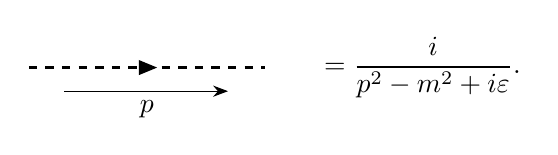
\begin{tikzpicture}
        \begin{feynman}
            \vertex (a) at (0,0);
            \vertex (b) at (3,0);
            \draw [dashed, with arrow=0.5, thick, momentum'=$p$] (a) -- (b); % Dashed line with arrow
            \node at (5,0) {$\displaystyle =\frac{i}{p^2 - m^2 + i\varepsilon}.$};
        \end{feynman}
    \end{tikzpicture}
\end{center}
This propagator propagates both $\phi$ and $\phi^*$, that is, both particles and antiparticles at the same time; they cannot be disentangled!

The photon propagator was calculated in the last chapter:
\begin{center}
    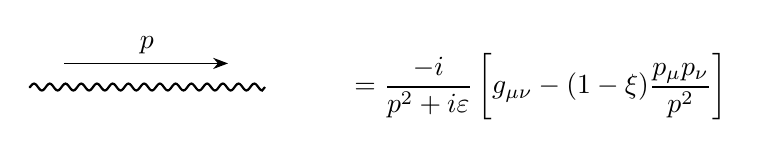
\begin{tikzpicture}
        \begin{feynman}
            \vertex (a) at (0,0);
            \vertex (b) at (3,0);
            % Corrected momentum arrow syntax:
            \diagram*{
            (a) -- [boson, momentum={$p$}, thick] (b),
            };
            % Propagator equation with proper spacing
            \node at (6.5,0) {$\displaystyle =\frac{-i}{p^2+ i\varepsilon}\left[g_{\mu\nu} -(1-\xi)\frac{p_\mu p_\nu}{p^2}\right]$};
        \end{feynman}
    \end{tikzpicture}
\end{center}

Notice that some of the interactions involve derivatives of $\phi, \phi^*$ and $A_\mu$, which will produce momentum factors. Recall that $\phi$ creates an antiparticle or destroys a particle, and $\phi^*$ creates a particle or destroys an antiparticle. When a derivative acts on these fields, we will have an extra factor of $\pm ip_\mu$.

The interaction has the form
\begin{equation}
    -ieA_\mu [\phi^*(\partial_\mu\phi) - (\partial_\mu\phi^*)\phi],
\end{equation}
it always has one derivative on both $\phi$ and $\phi^*$. Each $p^\mu$ comes with an $i$, and the expansion of $\exp(i\mathcal{L}_\text{int})$ gives another $i$ for each vertex, so we always get an $(-ie)i^2 = ie$ multiplying the $\pm p^\mu$ factor coming from the derivative. We will now explore all four possible vertices (another four-point vertex will be discussed later):
\begin{enumerate}
    \item Annihilate $e^-$ and create $e^-$: particle scattering
    \begin{center}
    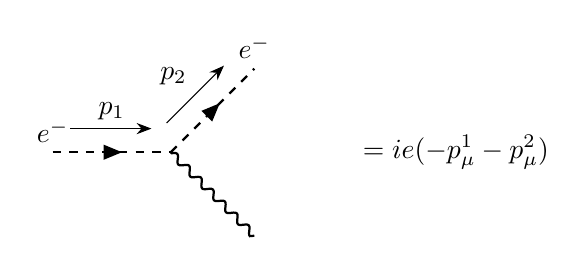
\begin{tikzpicture}
        \begin{feynman}
            \vertex [label=$e^{-}$] (i); % Labeled initial electron
            \vertex [right= of i] (a);
            \vertex [above right= of a, label=$e^{-}$] (f1); % Labeled final electron
            \vertex [below right= of a] (f2);
            \vertex [above right= of f2] (w0);
            \vertex [right= of w0] (w);

            \diagram*{
                (i) --[dashed, with arrow=0.5, momentum=$p_1$, thick] (a),
                (a) --[dashed, with arrow=0.5, momentum=$p_2$, thick] (f1);
                (a) --[photon, thick] (f2),
            };

            \node at (w) {$\displaystyle = ie(-p_\mu^1 - p_\mu^2)$};
        \end{feynman}
    \end{tikzpicture}
    \end{center}
    The $\phi^*(\partial_\mu\phi)$ annihilates an $e^-$, which gives a $-p_\mu^1$, and the $-(\partial_\mu\phi^*)\phi$ creates an $e^-$, which gives a $-(+p_\mu^2)$.
    \item Annihilate $e^+$ and create $e^+$: antiparticle scattering
    \begin{center}
    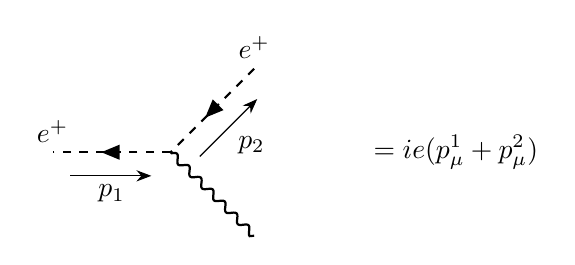
\begin{tikzpicture}
        \begin{feynman}
            \vertex [label=$e^{+}$] (i); % Labeled initial electron
            \vertex [right= of i] (a);
            \vertex [above right= of a, label=$e^{+}$] (f1); % Labeled final electron
            \vertex [below right= of a] (f2);
            \vertex [above right= of f2] (w0);
            \vertex [right= of w0] (w);

            \diagram*{
                (a) --[dashed, with arrow=0.5, thick] (i),
                (i) --[opacity=0, momentum'=$p_1$, thick] (a),
                (f1) --[dashed, with arrow=0.5, thick] (a),
                (a) --[opacity=0, momentum'=$p_2$, thick] (f1),
                (a) --[photon, thick] (f2),
            };
            \node at (w) {$\displaystyle = ie(p_\mu^1 + p_\mu^2)$};
        \end{feynman}
    \end{tikzpicture}
    \end{center}
    The $-(\partial_\mu\phi^*)\phi$ annihilates an $e^+$, which gives a $-(-p_\mu^1)$, and the $\phi^*(\partial_\mu\phi)$ creates an $e^+$, which gives a $p_\mu^2$.
    \item Annihilate $e^-$ and annihilate $e^+$: pair annihilation
    \begin{center}
    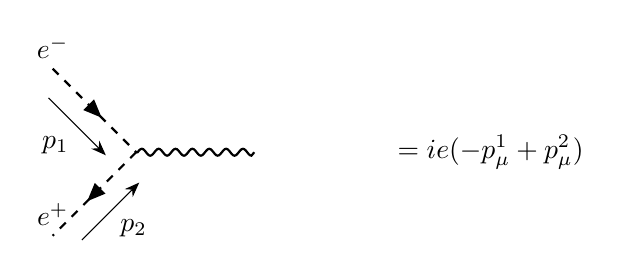
\begin{tikzpicture}
        \begin{feynman}
            \vertex (a);
            \vertex [above left= of a,label=$e^{-}$] (i1); % Labeled initial electron
            \vertex [below left= of a, label=$e^{+}$] (i2); % Labeled final electron
            \vertex [right= of a] (f);
            \vertex [right= of f] (w0);
            \vertex [right= of w0] (w);

            \diagram*{
                (i1) --[dashed, with arrow=0.5, thick] (a),
                (i1) --[opacity=0, momentum'=$p_1$, thick] (a),
                (a) --[dashed, with arrow=0.5, thick] (i2),
                (i2) --[opacity=0, momentum'=$p_2$, thick] (a),
                (a) --[photon, thick] (f),
            };
            \node at (w) {$\displaystyle = ie(-p_\mu^1 + p_\mu^2)$};
        \end{feynman}
    \end{tikzpicture}
    \end{center}
    The $-(\partial_\mu\phi^*)\phi$ annihilates an $e^+$, which gives a $-(-p_\mu^2)$, and the $\phi^*(\partial_\mu\phi)$ annihilates an $e^-$, which gives a $-p_\mu^1$.
    \item Create $e^+$ and create $e^-$: pair production
    \begin{center}
    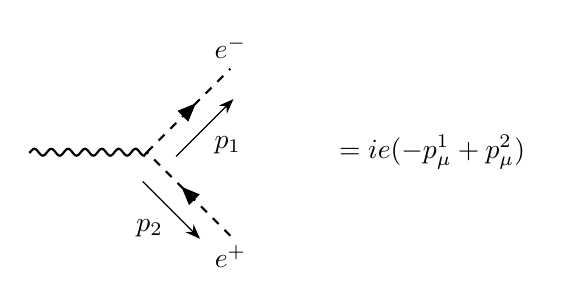
\begin{tikzpicture}
        \begin{feynman}
            \vertex (i); % Labeled initial electron
            \vertex [right= of i] (a);
            \vertex [above right= of a, label=$e^{-}$] (f1); % Labeled final electron
            \vertex [below right= of a, label=below:$e^{+}$] (f2);
            \vertex [above right= of f2] (w0);
            \vertex [right= of w0] (w);

            \diagram*{
                (a) --[dashed, with arrow=0.5, thick] (f1),
                (a) --[opacity=0, momentum'=$p_1$, thick] (f1),
                (f2) --[dashed, with arrow=0.5, thick] (a),
                (a) --[opacity=0, momentum'=$p_2$, thick] (f2),
                (i) --[photon, thick] (a),
            };
            \node at (w) {$\displaystyle = ie(-p_\mu^1 + p_\mu^2)$};
        \end{feynman}
    \end{tikzpicture}
    \end{center}
    The $-(\partial_\mu\phi^*)\phi$ creates an $e^-$, which gives a $-p_\mu^1$, and the $\phi^*(\partial_\mu\phi)$ creates an $e^+$, which gives a $p_\mu^2$.
\end{enumerate}
In the above diagrams, we have used particle-flow arrows to distinguish electrons and positrons, which points in the direction of momentum for electrons ($e^-$) and opposite to the direction of momentum for positrons ($e^+$). Historically, antiparticles are interpreted as particles going backward in time. We have inherited the notion of using a left-pointing particle-flow arrow in our diagrams.

By observing all vertices, one would notice that if the momentum-flow arrow points to the right, the vertex gives $-iep_\mu$, if the particle-flow points to the left, the vertex gives $+iep_\mu$. Therefore, another Feynman rule for the scalar QED would be:
\begin{shaded}
    A scalar QED vertex gives $-ie$ times the sum of the momentum of the particles whose particle-flow arrows point to the right minus the momentum of the particles whose arrows point to the left.
\end{shaded}
Particle-flow arrows should always make a connected path through the Feynman diagram. The direction of the arrows is arbitrary for the internal lines; as long as the direction of the arrows is consistent with the particle-flow, the answer will come out the same.

One should also notice, that there is another type of interaction in the scalar QED, the 4-point vertex:
\begin{equation}
    \mathcal{L}_\text{int} = e^2 A_\mu^2 \abs{\phi}^2 = e^2 g_{\mu\nu} A_\mu A_\nu \abs{\phi}^2
\end{equation}
which corresponds to the vertex
\begin{center}
    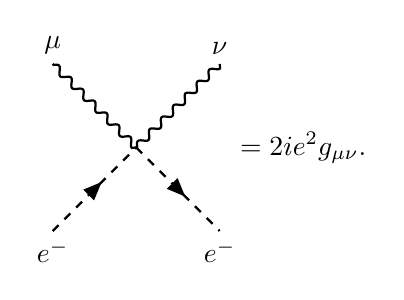
\begin{tikzpicture}
        \begin{feynman}
            \vertex [label = $\mu$] (i1);
            \vertex [below right=of i1] (a);
            \vertex [below left=of a, label = below:$e^-$] (i2);
            \vertex [below right=of a, label = below:$e^-$] (f2);
            \vertex [above right=of a, label = $\nu$] (f1);
            \vertex [below right = of f1] (eq);

            \diagram* {
                (i1) --[photon, thick] (a),
                (a) --[photon, thick] (f1),
                (a) --[dashed, with arrow=0.5, thick] (f2),
                (i2) --[dashed, with arrow=0.5, thick] (a),
            };

            \node at (eq) {$\displaystyle = 2ie^2g_{\mu\nu}.$};
        \end{feynman}
    \end{tikzpicture}
\end{center}
This is also known as the seagull vertex. The $i$ comes from the expansion of $\exp(i\mathcal{L}_\text{int})$ which we always have in the Feynman rules. The 2 comes from the symmetry factor for the two $A_\mu$ fields.

\subsubsection{External Vertices}
Now we know the vertex factors and propagators for the photon and the complex scalar field. We are left to handle the external vertices, so we have the complete set of Feynman rules. It is easy for the real scalar field, we simply get a factor of 1. The complex scalar field is just two real scalar fields. Thus, we also get a factor of 1. Things get a bit more subtle with the external photons,
Recall the photon field is given by
\begin{equation}
    A_\mu(x) = \int\frac{d^3p}{(2\pi)^3}\frac{1}{\sqrt{2\omega_p}}\sum_{j=1}^2(\epsilon_\mu^j(p)a_{p,j}e^{-ipx} + \epsilon_\mu^{j*}(p)a_{p,j}^\dagger e^{ipx}),
\end{equation}
which is just a bunch of scalar fields integrated with the polarization vectors $\epsilon_\mu^i(p)$. Recall that external states with photons have momenta and polarizations, $\ket{k, \epsilon}$, so that $\bra{0}A_\mu(x)\ket{p, \epsilon_i} = \epsilon_\mu ^i(p) e^{-ipx}$. This leads to LSZ being modified only by adding a factor of the polarization for each external state: $\epsilon_\mu ^i(p)$ for incoming photons and $\epsilon_\mu ^{i*}(p)$ for outgoing photons.

\begin{tcolorbox}[breakable, colback=yellow!20!white, colframe=black, boxrule=1pt]
To see the above argument more explicitly, recall the key to proving the LSZ reduction formula is the identity:
\begin{equation}
    i\int d^4x e^{ipx}(\square+m^2)\phi(x) = \sqrt{2\omega_p}[a_p(\infty) - a_p(-\infty)].
\end{equation}
For the photon field, we should try to evaluate 
\begin{equation}
    i\int d^4x e^{ipx}\square A_\mu(x).
\end{equation}
Following the same steps from the real scalar field case, we would get
\begin{equation}
    i\int d^4x e^{ipx}\square A_\mu(x) = \partial_t \int dt e^{i\omega_pt} \int d^3x e^{-i\vec{p}\vec{x}}(i\partial_t+ \omega_p) A_\mu(x).
\end{equation}
Then, in the scalar field case, by expanding $\phi(x)$ in terms of creation and annihilation operators, we find
\begin{equation}
    \int d^3x e^{-i\vec{p}\vec{x}}(i\partial_t+ \omega_p) \phi(x) = \sqrt{2\omega_p}a_p(t)e^{-i\omega_pt}.
\end{equation}
However, for $A_\mu(x)$, the expansion includes polarization vectors, and thus
\begin{equation}
    \int d^3x e^{-i\vec{p}\vec{x}}(i\partial_t+ \omega_p) A_\mu(x) = \sqrt{2\omega_p} \sum_{j=1}^2 \epsilon_\mu^j(p) a_{p,j}(t)e^{-i\omega_pt}.
\end{equation}
Hence, 
\begin{equation}
    i\int d^4x e^{ipx}\square A_\mu(x) = \sqrt{2\omega_p} \sum_{j=1}^2 \epsilon_\mu^j(p) [a_{p,j}(\infty) - a_{p,j}(-\infty)].
\end{equation}
To get rid of the polarization vectors in the result, recall that $\epsilon_{i}^{\mu*}\epsilon_j^\mu = -\delta_{ij}$. Therefore, we can multiply $\epsilon_\mu^i$ on both sides to get
\begin{equation}
    i\epsilon_\mu^{i*}\int d^4x e^{ipx}\square A_\mu(x) = -\sqrt{2\omega_p} [a_{p,i}(\infty) - a_{p,i}(-\infty)].
\end{equation}
Taking the complex conjugate, we have
\begin{equation}
    i\epsilon_\mu^{i}\int d^4x e^{-ipx}\square A_\mu(x) = -\sqrt{2\omega_p} [a_{p,i}^\dagger(\infty) - a_{p,i}^\dagger(-\infty)].
\end{equation}
Thus, for photon fields, we get an extra factor of $\epsilon^{i*}_\mu$ for outgoing photons and $\epsilon^{i}_\mu$ for incoming photons. Note, as we will take the modulus square of the matrix element, so the extra minus sign does not matter.
\end{tcolorbox}
\subsection{Scattering in Scalar QED}
Let us calculate the cross section for Møller scattering, $e^-e^-\rightarrow e^-e^-$, in scalar QED. There are two diagrams that contribute to the tree-level. The $t$-channel diagram:
\begin{center}
    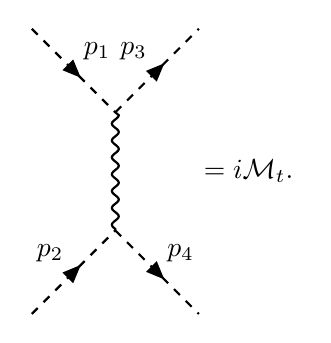
\begin{tikzpicture}
        \usetikzlibrary{calc} % 启用坐标计算库
        \begin{feynman}
            \vertex (i1);
            \vertex [below right=1.5cm of i1] (a); % 增加距离避免标签重叠
            \vertex [below=1.5cm of a] (b);
            \vertex [below left=1.5cm of b] (i2);
            \vertex [above right=1.5cm of a] (f1);
            \vertex [below right=1.5cm of b] (f2);
            % 计算 a 和 b 的中点作为公式位置
            \coordinate (midpoint) at ($(a)!0.5!(b)$);

            \diagram* {
            (i1) --[dashed, with arrow=0.5, thick, edge label=\(p_1\)] (a), % 调整位置
            (i2) --[dashed, with arrow=0.5, thick, edge label=\(p_2\)] (b), % 调整位置
            (b) --[photon, thick] (a),
            (a) --[dashed, with arrow=0.5, thick, edge label=\(p_3\)] (f1),
            (b) --[dashed, with arrow=0.5, thick, edge label=\(p_4\)] (f2),
            };
            % 将公式置于中轴线 (midpoint) 右侧
            \node [right=1cm] at (midpoint) {\(\displaystyle=i\mathcal{M}_t.\)};
        \end{feynman}
    \end{tikzpicture}
\end{center}
Thus,
\begin{equation}
    i\mathcal{M}_t = (-ie)(p_1^\mu + p_3^\mu)\frac{-i\left[ g_{\mu\nu} - (1-\xi)\frac{k_\mu k_\nu}{k^2}\right]}{k^2}(-ie)(p_2^\nu + p_4^\nu),
\end{equation}
where $k^\mu = p_3^\mu - p_1^\mu$ according to momentum conservation. Therefore,
\begin{equation}
    k^\mu(p_1^\mu + p_3^\mu) = (p_3^\mu - p_1^\mu)(p_1^\mu + p_3^\mu) = m^2 - m^2 = 0.
\end{equation}
We find
\begin{equation}
    \mathcal{M}_t =\frac{e^2(p_1^\mu + p_3^\mu)(p_2^\mu + p_4^\mu)}{t},
\end{equation}
which is independent of $\xi$ as expected (gauge invariance). 

Another possible diagram would be the $u$-channel:
\begin{center}
    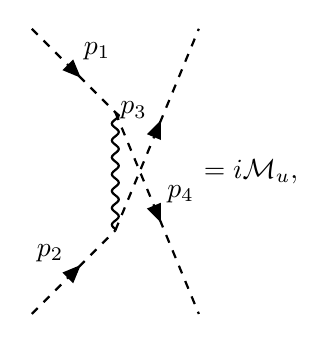
\begin{tikzpicture}
        \usetikzlibrary{calc} % 启用坐标计算库
        \begin{feynman}
            \vertex (i1);
            \vertex [below right=1.5cm of i1] (a); % 增加距离避免标签重叠
            \vertex [below=1.5cm of a] (b);
            \vertex [below left=1.5cm of b] (i2);
            \vertex [above right=1.5cm of a] (f1);
            \vertex [below right=1.5cm of b] (f2);
            % 计算 a 和 b 的中点作为公式位置
            \coordinate (midpoint) at ($(a)!0.5!(b)$);

            \diagram* {
            (i1) --[dashed, with arrow=0.5, thick, edge label=\(p_1\)] (a), % 调整位置
            (i2) --[dashed, with arrow=0.5, thick, edge label=\(p_2\)] (b), % 调整位置
            (b) --[photon, thick] (a),
            (a) --[dashed, with arrow=0.5, thick, edge label=\(p_4\)] (f2),
            (b) --[dashed, with arrow=0.5, thick, edge label=\(p_3\)] (f1),
            };
            % 将公式置于中轴线 (midpoint) 右侧
            \node [right=1cm] at (midpoint) {\(\displaystyle=i\mathcal{M}_u,\)};
        \end{feynman}
    \end{tikzpicture}
\end{center}
which gives
\begin{equation}
    i\mathcal{M}_u = (-ie)(p_1^\mu + p_4^\mu)\frac{-i\left[ g_{\mu\nu} - (1-\xi)\frac{k_\mu k_\nu}{k^2}\right]}{k^2}(-ie)(p_2^\nu + p_3^\nu)
\end{equation}
with $k^\mu = p_4^\mu - p_1^\mu$. Similarly, we have
\begin{equation}
    k^\mu(p_1^\mu + p_4^\mu) = (p_4^\mu - p_1^\mu)(p_1^\mu + p_4^\mu) = m^2 - m^2 = 0.
\end{equation}
Thus, we have
\begin{equation}
    \mathcal{M}_u =\frac{e^2(p_1^\mu + p_4^\mu)(p_2^\mu + p_3^\mu)}{u}.
\end{equation}
Note that by simply interchanging $3 \leftrightarrow 4$, we can go from the $u$-channel to the $t$-channel.

Now, putting everything together, the cross section of the Møller scattering at tree-level is
\begin{equation}
\begin{aligned}
        \frac{d\sigma(e^-e^- \rightarrow e^-e^-)}{d\Omega} &= \frac{e^4}{64\pi^2E_\text{CM}^2}\left[\frac{(p_1^\mu + p_4^\mu)(p_2^\mu + p_3^\mu)}{u} +  \frac{(p_1^\mu + p_3^\mu)(p_2^\mu + p_4^\mu)}{t}\right]^2\\
        &= \frac{\alpha^2}{4s}\left[\frac{s-u}{u} +  \frac{s-t}{t}\right]^2,
\end{aligned}
\end{equation}
where $\alpha= \frac{e^2}{4\pi}$ is the fine-structure constant.

\subsection{Ward Identity and Gauge Invariance}
In the previous example, we saw that the $\xi$ term vanishes, as expected by gauge invariance. A general matrix element involving a photon propagator would be $M_{\mu\nu}\Pi_{\mu\nu}$. So gauge invariance requires $M_{\mu\nu}p_\mu p_\nu$ to vanish, which is closely related to the Ward identity. The ward identity states that ,for a matrix element involving an on-shell photon $\epsilon_\mu M_\mu$, $p_\mu M_\mu = 0$. Both gauge invariance and Ward identity are tedious to prove in perturbation theory. The general proof would be given later using the path integral. The actual diagrammatic proof would be easier in the real QED, since there is no 4-point vertex involved.

\subsection{Lorentz Invariance and Charge Conservation}
There is a beautiful and direct connection between Lorentz invariance and charge conservation that bypasses gauge invariance completely. What we will now show is that a theory with a massless spin-1 particle automatically has an associated conserved charge. This profound result, due to Steven Weinberg, does not require a Lagrangian description: it only uses little-group invariance and the fact that for a massless field, one can take the soft limit (the soft photon theorem). The soft-photon theorem by Weinberg provides a mathematical framework for analysing the scattering of particles with soft photons, which are photons whose energy is taken to zero.

We will start by considering a diagram with many external legs, loops and etc. Say the matrix element of this process is $\mathcal{M}_0$. Let us focus on an outgoing photon with momentum $q^\mu$ and polarization $\epsilon^{\mu*}$, which we will tack on an external incoming electron with index $i$:

\begin{center}
    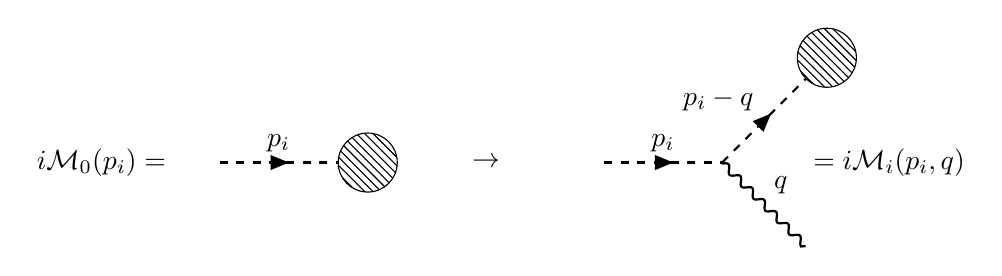
\begin{tikzpicture}
        \begin{feynman}
            \vertex (i);
            \vertex [right= of i, blob] (M) {};
            \vertex [left = of i] (eq);
            \vertex[right = of M] (a);
            \vertex[right = of a] (a1);
            \vertex[right = of a1] (b);
            \vertex[above right = of b, blob] (c) {};
            \vertex[below right = of b] (d);
            \vertex[above right= of d] (M1);
            \diagram* {
            (i) --[dashed, with arrow=0.5, edge label = $p_i$, thick] (M),
            (M) --[opacity=0] (a),
            };
            \node at (eq) {$\displaystyle i\mathcal{M}_0(p_i)=$};
            \node at (a) {$\displaystyle\rightarrow$};
            \diagram* {
            (a1) --[dashed, with arrow=0.5, edge label = $p_i$, thick] (b),
            (b) --[dashed, with arrow=0.5, edge label = $p_i-q$, thick] (c),
            (b) --[photon, thick, edge label = $q$] (d),
            };
            \node at (M1) {$\displaystyle =i\mathcal{M}_i(p_i,q)$};
        \end{feynman}
        
    \end{tikzpicture}
\end{center}
Thus the matrix element $\mathcal{M}_0$ is given by
\begin{equation}
    \mathcal{M}_0(p_i,q) = (-ie)\frac{i(2p_i^\mu-q^\mu)}{(p_i-q)^2 - m^2}\epsilon_\mu^*\mathcal{M}_0(p_i-q).
\end{equation}
Using $p_i^2 = m^2$ and $q^2=0$ $q \cdot \epsilon^*=0$ for on-shell photon, we find
\begin{equation}
    \mathcal{M}_0(p_i,q) = -e\frac{p_i \cdot \epsilon^*}{p_i \cdot q}\mathcal{M}_0(p_i-q).
\end{equation}
Now we can take the soft limit. To specify, by soft limit, we mean that $\abs{q\cdot p_i} \ll \abs{p_j \cdot p_k}$ for all external legs $p_i$. Then, we should have $\mathcal{M}_0(p_i) \approx \mathcal{M}_0(p_i-q)$, where $\approx$ is often used to denote the soft limit. Hence,
\begin{equation}
    \mathcal{M}_0(p_i,q) \approx -e\frac{p_i \cdot \epsilon^*}{p_i \cdot q}\mathcal{M}_0(p_i).
\end{equation}
Also, notice that the photon attached to loop momenta in the blob is subdominant. This is because these photons are off-shell, and thus $q^2 \neq 0$. This means that these photons cannot give factor of $\frac{1}{q\cdot p}$. Therefore, in the soft limit ($q\rightarrow 0$), the photons coming from the loops does not produce singularity. In conclusion, under the soft limit, the dominant effect comes from photons attached to external legs, and we should sum over all such diagrams.

If the external leg is an incoming $e^+$ instead of $e^-$, we would get
\begin{equation}
    \mathcal{M}_0(p_i,q) \approx e\frac{p_i \cdot \epsilon^*}{p_i \cdot q}\mathcal{M}_0(p_i).
\end{equation}

If the external leg now becomes an outgoing $e^-$, the diagram becomes
\begin{center}
    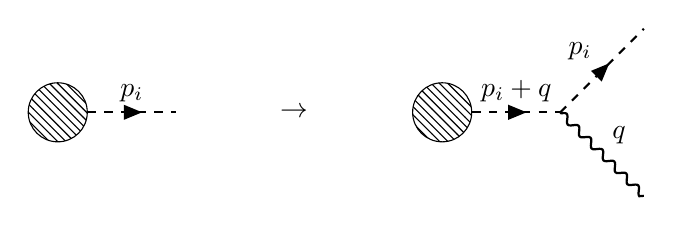
\begin{tikzpicture}
        \begin{feynman}
            \vertex [blob] (i) {};
            \vertex [right= of i] (M);
            \vertex [left = of i] (eq);
            \vertex[right = of M] (a);
            \vertex[right = of a, blob] (a1) {};
            \vertex[right = of a1] (b);
            \vertex[above right = of b] (c);
            \vertex[below right = of b] (d);
            \vertex[above right= of d] (M1);
            \diagram* {
            (i) --[dashed, with arrow=0.5, edge label = $p_i$, thick] (M),
            (M) --[opacity=0] (a),
            };
            \node at (a) {$\displaystyle\rightarrow$};
            \diagram* {
            (a1) --[dashed, with arrow=0.5, edge label = $p_i+q$, thick] (b),
            (b) --[dashed, with arrow=0.5, edge label = $p_i$, thick] (c),
            (b) --[photon, thick, edge label = $q$] (d),
            };
        \end{feynman}
        
    \end{tikzpicture}
\end{center}
and the amplitude is modified to be
\begin{equation}
    \mathcal{M}_0(p_i,q) = (-ie)\frac{i(2p_i^\mu+q^\mu)}{(p_i+q)^2 - m^2}\epsilon_\mu^*\mathcal{M}_0(p_i+q).
\end{equation}
Similarly, this can be simplified as
\begin{equation}
    \mathcal{M}_0(p_i,q) \approx e\frac{p_i \cdot \epsilon^*}{p_i \cdot q}\mathcal{M}_0(p_i).
\end{equation}
For an outgoing photon, we would have another sign flip, and thus
\begin{equation}
    \mathcal{M}_0(p_i,q) \approx -e\frac{p_i \cdot \epsilon^*}{p_i \cdot q}\mathcal{M}_0(p_i).
\end{equation}

If we had many charges with different charge $Q_i$, we would have
\begin{equation}
    \mathcal{M} \approx e\mathcal{M}_0\left[ \sum_\text{incoming}Q_i\frac{p_i \cdot \epsilon^*}{p_i \cdot q} - \sum_\text{outgoing}Q_i\frac{p_i \cdot \epsilon^*}{p_i \cdot q} \right].
\end{equation}

Now, we perform a Lorentz transformation, which takes $\mathcal{M}(p_i, \epsilon_i) \rightarrow \mathcal{M}(p_i', \epsilon_i')$. Recall that the polarization vector does not transform like a 4-vector. There are some little group transformations, which
\begin{equation}
    \epsilon_\mu \rightarrow \epsilon_\mu + q_\mu.
\end{equation}
Thus, 
\begin{equation}
    \mathcal{M} \rightarrow \mathcal{M} + e\mathcal{M}_0\left[ \sum_\text{incoming}Q_i - \sum_\text{outgoing}Q_i \right].
\end{equation}
Since $\mathcal{M}$ is Lorentz-invariant, we must have
\begin{shaded}
    \begin{equation}
         \sum_\text{incoming}Q_i = \sum_\text{outgoing}Q_i,
    \end{equation}
\end{shaded}
which is precisely charge conservation. Since this process was completely arbitrary, we can conclude that charge must always be conserved.

Although, the above derivation was completely based on the scalar QED, it is completely general. We can suppose the photon has an arbitrary interaction with $\phi$. Then the Feynman rule for the vertex would have an arbitrary dependence on momenta:
\begin{center}
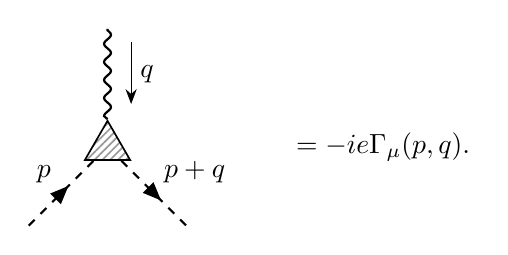
\begin{tikzpicture}[
    triangle vertex/.style={
        regular polygon, 
        regular polygon sides=3,
        minimum size=6mm,  % 增大尺寸确保覆盖
        fill=white,        % 白色不透明底
        pattern={Lines[angle=45,distance=2pt]},
        pattern color=black!40,
        draw=black,        % 黑色边框
        line width=0.6pt
    }
]
    \begin{feynman}
        % 先定义顶点位置
        \vertex (a) at (0, 0);
        \vertex (b) at (0, -1.5);  % 明确指定位置
        \vertex (c) at (-1, -2.5);
        \vertex (d) at (1, -2.5);
        \vertex (eq) at (3.5, -1.5) {$\displaystyle=-ie\Gamma_\mu(p,q).$};
        
        % 先绘制三角形顶点（在最上层）
        \node at (b) [triangle vertex] (vertex) {};
        
        % 后绘制连线，连接到三角形边界
        \diagram*{
            (a) --[photon, thick, momentum = $q$] (vertex.north),  % 连接到上边界
            (c) --[charged scalar, thick, edge label = $p$] (vertex.south west),  % 连接到左下角
            (vertex.south east) --[charged scalar, thick, edge label = $p+q$] (d),  % 连接到右下角
        };
    \end{feynman}
\end{tikzpicture}
\end{center}
The matrix element must be Lorentz-invariant, therefore the vertex must have a $\mu$ index to contract with the polarization. Meanwhile, also by Lorentz invariance, we can write $\Gamma^\mu$ as
\begin{equation}
    \Gamma^\mu (p,q) = 2p^\mu F(p^2,q^2,p\cdot q) + q^\mu G (p^2,q^2,p\cdot q),
\end{equation}
where $F$ and $G$ are known as the form factors. In scalar QED, $F=G=1$. As the photon is on-shell, we have $q_\mu\epsilon_\mu = 0$ just as before. Therefore, we can ignore $G$. Also, we have $q^2=0$ and $p^2 = m^2$. Thus, 
\begin{equation}
    \Gamma^\mu (p,q) = 2p^\mu F\left(\frac{p\cdot q}{m^2}\right),
\end{equation}
which we can now put this more general form into the above argument.

Similarly, consider the diagram

\begin{center}
    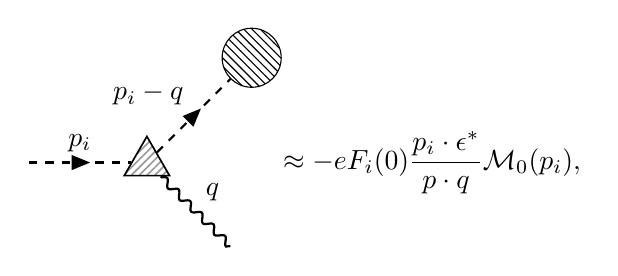
\begin{tikzpicture}[
    triangle vertex/.style={
        regular polygon, 
        regular polygon sides=3,
        minimum size=6mm,  % 增大尺寸确保覆盖
        fill=white,        % 白色不透明底
        pattern={Lines[angle=45,distance=2pt]},
        pattern color=black!40,
        draw=black,        % 黑色边框
        line width=0.6pt
    }
]
        \begin{feynman}
            \vertex (a1);
            \vertex[right = of a1] (b);
            \vertex[above right = of b, blob] (c) {};
            \vertex[below right = of b] (d);
            \vertex[above right= of d] (M1);
            \vertex[right= of M1] (M2);
            
            \node at (b) [triangle vertex] (vertex) {};
            
            \diagram* {
            (a1) --[dashed, with arrow=0.5, edge label = $p_i$, thick] (vertex.west),
            (vertex.north east) --[dashed, with arrow=0.5, edge label = $p_i-q$, thick] (c),
            (vertex.south east) --[photon, thick, edge label = $q$] (d),
            };
            \node at (M2) {$\displaystyle \approx -eF_i(0)\frac{p_i \cdot \epsilon^*}{p \cdot q}\mathcal{M}_0(p_i),$};
        \end{feynman}
        
    \end{tikzpicture}
\end{center}
where we have taken the soft limit, so that $F_i\left(\frac{p\cdot q}{m^2}\right) \approx F_i(0)$. Note that we have added the index $i$ to indicate different particles. Although $F_i$ does not have to be an analytic function, it should be finite as $q \rightarrow 0$, otherwise the matrix element would diverge when emitting a soft photon. Then, to satisfy Lorentz invariance under the little group transformation, we must have
\begin{equation}
    \sum_\text{incoming}F_i(0) = \sum_\text{outgoing}F_i(0).
\end{equation}
Note, we have produced a more general definition for the charge $Q_i=-F_i(0)$.

The above derivation was completely general. More specifically, the interaction between photon and any charged particle always has the form $\frac{p \cdot \epsilon^*}{p \cdot q}$. Therefore,
\begin{center}
\begin{shaded}
        Massless spin-1 particles imply charge conservation!
\end{shaded}
\end{center}
Remember, the masslessness of the photon is crucial: there are only two polarizations, and we can take the soft limit with the photon on-shell.

To repeat, this is a non-perturbative statement about the physical universe, not merely a statement about our computation methods, like gauge invariance and the Ward identities. Proofs of this nature are rare and extremely powerful.

\subsubsection{Lorentz Invariance for Spin 2 and Higher}
A massless spin-2 field has two polarizations $\epsilon_{\mu\nu}^i$, which rotate into each other under Lorentz transformations, and also into $q_\mu q_\nu$. There are little-group transformations that send
\begin{equation}
    \epsilon_{\mu\nu} \rightarrow \epsilon_{\mu\nu} + \Lambda_\mu q_\nu + \Lambda_\nu q_\mu + \Lambda q_\mu q_\nu,
\end{equation}
where $\Lambda_\mu$ has to do with the specific way the Lorentz group acts. With similar reasoning for massless spin-1 particle, a massless spin-2 particle should also satisfy the Ward identity: if we replace even one polarization tensor index by $q_\mu$, the matrix element should vanish. The spin-2 polarizations can be projected out of $\epsilon_{\mu\nu}$ as the transverse-traceless modes: $q_\mu \epsilon_{\mu\nu} = \epsilon_{\mu\mu} = 0$.

We can write down the general interaction
\begin{center}
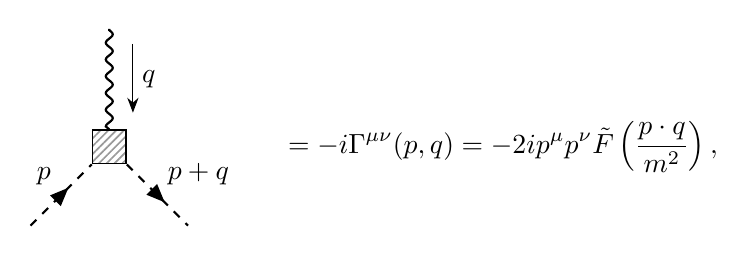
\begin{tikzpicture}[
    square vertex/.style={
        regular polygon, 
        regular polygon sides=4,
        minimum size=6mm,  % 增大尺寸确保覆盖
        fill=white,        % 白色不透明底
        pattern={Lines[angle=45,distance=2pt]},
        pattern color=black!40,
        draw=black,        % 黑色边框
        line width=0.6pt
    }
]
    \begin{feynman}
        % 先定义顶点位置
        \vertex (a) at (0, 0);
        \vertex (b) at (0, -1.5);  % 明确指定位置
        \vertex (c) at (-1, -2.5);
        \vertex (d) at (1, -2.5);
        \vertex (eq) at (5, -1.5) {$\displaystyle=-i\Gamma^{\mu\nu}(p,q) = -2ip^\mu p^\nu \tilde{F}\left(\frac{p\cdot q}{m^2}\right),$};
        
        % 先绘制三角形顶点（在最上层）
        \node at (b) [square vertex] (vertex) {};
        
        % 后绘制连线，连接到三角形边界
        \diagram*{
            (a) --[photon, thick, momentum = $q$] (vertex.north),  % 连接到上边界
            (c) --[charged scalar, thick, edge label = $p$] (vertex.south west),  % 连接到左下角
            (vertex.south east) --[charged scalar, thick, edge label = $p+q$] (d),  % 连接到右下角
        };
    \end{feynman}
\end{tikzpicture}
\end{center}
where we required to tensor index to contract with $\epsilon_{\mu\nu}$.

Now, taking the soft limit and adding up diagrams, we have
\begin{equation}
    \mathcal{M} = \mathcal{M}_0\left[ \sum_\text{incoming}\tilde{F}_i(0) \frac{p_i^\mu}{p_i\cdot q} \epsilon_{\mu\nu}p_i^\nu -  \sum_\text{outgoing}\tilde{F}_i(0) \frac{p_i^\mu}{p_i\cdot q} \epsilon_{\mu\nu}p_i^\nu \right].
\end{equation}

Now, under a little-group transformation which brings $\epsilon_{\mu\nu} \rightarrow \epsilon_{\mu\nu} + q_\mu \Lambda_\nu$, we find
\begin{equation}
    \mathcal{M} \rightarrow \mathcal{M} + \mathcal{M}_0\Lambda_\nu \left[ \sum_\text{incoming}\tilde{F}_i(0) p_i^\nu -  \sum_\text{outgoing}\tilde{F}_i(0) p_i^\nu \right].
\end{equation}
By Lorentz invariance, we require
\begin{equation}
    \sum_\text{incoming}\tilde{F}_i(0) p_i^\nu = \sum_\text{outgoing}\tilde{F}_i(0) p_i^\nu. 
\end{equation}
This means $\tilde{F}_i(0) p_i^\nu$ is conserved, but we already knew that momentum itself is conserved. Therefore, we must have
\begin{equation}
    \tilde{F}_i(0) = \kappa \quad \forall i,
\end{equation}
where $\kappa$ is a constant. This is gravity! All particles gravitate with the same strength, $\kappa \equiv \frac{1}{M_\text{Pl}} = \sqrt{G_n}$. In other words, gravity is universal. So,
\begin{center}
    \begin{shaded}
        Massless spin-2 particles imply that gravity is universal.
    \end{shaded}
\end{center}
What if we keep going? By analogy, for spin-3 we should have
\begin{equation}
     \sum_\text{incoming}\hat{F}_i(0) p_i^\nu p_i^\mu = \sum_\text{outgoing}\hat{F}_i(0) p_i^\nu p_i^\mu.
\end{equation}
For example, if we take $\mu=\nu=0$, we find
\begin{equation}
    \sum_\text{incoming}\hat{F}_i(0) E_i^2 = \sum_\text{outgoing}\hat{F}_i(0) E_i^2.
\end{equation}
The only way to satisfy this, is if all the charges are 0. Therefore,
\begin{center}
    \begin{shaded}
        There are no interacting theories of massless particles of spin greater than 2.
    \end{shaded}
\end{center}


\section{Spinors}
\subsection{Representations of the Lorentz Group}
We have tried to find unitary irreducible representations of the Poincaré group by writing down a Lagrangian with positive definite energy. The next logical step would be to find a way to systematically embed particles into fields. By doing this, we will reveal the existence of spin-$\frac{1}{2}$ particles.

\subsubsection{Group Theory}
A group is a set of elements $\{g_i\}$ and a rule $g_i \times g_j = g_k$ which tells how each set of elements is multiplied to get a third. More precisely, the rule needs to be associative, and there needs to be an identity group element and inverses. A representation is a particular embedding of these $g_i$ into operators that act on a vector space. Any group has the trivial representation $r: g_i \rightarrow \mathds{1}$. A representation in which each group element gets into its own matrix is called a faithful representation.
Recall Lorentz group preserves the Minkowski metric
\begin{equation}
    \Lambda^Tg\Lambda = g.
\end{equation}
The matrices in this equation are in 4-vector representation. Examples of Lorentz transformations are rotations around the \( x \), \( y \) or \( z \) axes:

\[
\begin{pmatrix}
1 & 0 & 0 & 0 \\
0 & 1 & 0 & 0 \\
0 & 0 & \cos\theta_x & \sin\theta_x \\
0 & 0 & -\sin\theta_x & \cos\theta_x
\end{pmatrix},
\quad
\begin{pmatrix}
1 & 0 & 0 & 0 \\
0 & \cos\theta_y & 0 & -\sin\theta_y \\
0 & 0 & 1 & 0 \\
0 & \sin\theta_y & 0 & \cos\theta_y
\end{pmatrix},
\quad
\begin{pmatrix}
1 & 0 & 0 & 0 \\
0 & \cos\theta_z & \sin\theta_z & 0 \\
0 & -\sin\theta_z & \cos\theta_z & 0 \\
0 & 0 & 0 & 1
\end{pmatrix}
\]

and boosts in the \( x \), \( y \) or \( z \) directions:

\[
\begin{pmatrix}
\cosh\beta_x & \sinh\beta_x & 0 & 0 \\
\sinh\beta_x & \cosh\beta_x & 0 & 0 \\
0 & 0 & 1 & 0 \\
0 & 0 & 0 & 1
\end{pmatrix},
\quad
\begin{pmatrix}
\cosh\beta_y & 0 & \sinh\beta_y & 0 \\
0 & 1 & 0 & 0 \\
\sinh\beta_y & 0 & \cosh\beta_y & 0 \\
0 & 0 & 0 & 1
\end{pmatrix},
\quad
\begin{pmatrix}
\cosh\beta_z & 0 & 0 & \sinh\beta_z \\
0 & 1 & 0 & 0 \\
0 & 0 & 1 & 0 \\
\sinh\beta_z & 0 & 0 & \cosh\beta_z
\end{pmatrix}.
\]

These matrices give an embedding of elements of the Lorentz group into a set of matrices. That is, they describe one particular representation of the Lorentz group (the 4-vector representation). We would now like to find all the representations.

To extract the group away from its representation, it is easiest to look at the infinitesimal transformations. In the 4-vector representation:
\begin{equation}
    \delta X_0 = \beta_i X_i,
\end{equation}
\begin{equation}
    \delta X_i = \beta_i X_i - \varepsilon_{ijk}\theta_j X_k.
\end{equation}
Generally, the infinitesimal transformations can be written as 
\begin{equation}
    \delta X_\mu = i\left[ \sum_{i=1}^3\theta_i(J_i)_{\mu\nu} + \beta_i(K_i)_{\mu\nu} \right]X_\nu,
\end{equation}
where

\[
J_1 = i\begin{pmatrix}
0 & 0 & 0 & 0 \\
0 & 0 & 0 & 0 \\
0 & 0 & 0 & -1 \\
0 & 0 & 1 & 0
\end{pmatrix}, \quad
J_2 = i\begin{pmatrix}
0 & 0 & 0 & 0 \\
0 & 0 & 0 & 1 \\
0 & 0 & 0 & 0 \\
0 & -1 & 0 & 0
\end{pmatrix}, \quad
J_3 = i\begin{pmatrix}
0 & 0 & 0 & 0 \\
0 & 0 & -1 & 0 \\
0 & 1 & 0 & 0 \\
0 & 0 & 0 & 0
\end{pmatrix},
\]

\[
K_1 = i\begin{pmatrix}
0 & -1 & 0 & 0 \\
-1 & 0 & 0 & 0 \\
0 & 0 & 0 & 0 \\
0 & 0 & 0 & 0
\end{pmatrix}, \quad
K_2 = i\begin{pmatrix}
0 & 0 & -1 & 0 \\
0 & 0 & 0 & 0 \\
-1 & 0 & 0 & 0 \\
0 & 0 & 0 & 0
\end{pmatrix}, \quad
K_3 = i\begin{pmatrix}
0 & 0 & 0 & -1 \\
0 & 0 & 0 & 0 \\
0 & 0 & 0 & 0 \\
-1 & 0 & 0 & 0
\end{pmatrix}.
\]
These matrices are known as the generators of the Lorentz group in the 4-vector basis. They generate the group in the sense that any element of the group can be written uniquely as
\begin{equation}
    \Lambda = \exp(i\theta_i J_i + i\beta_i K_i)
\end{equation}

up to some discrete transformations. The advantage of writing the group elements this way is that it is completely general. In any finite-dimensional representation the group elements can be written as an exponential of matrices.

For any group \( G \), some group elements \( g \in G \) can be written as \( g = \exp(i c_i^g \lambda_i) \), where \( c_i^g \) are numbers and \( \lambda_i \) are group generators. The generators are in an algebra, because you can add and multiply them, while the group elements are in a group, because you can only multiply them. For example, the real numbers form an algebra (there is a rule for addition and a rule for multiplication) but rotations are a group (there is only one rule, multiplication).

Lie groups are a class of groups, including the Lorentz group, with an infinite number of elements but a finite number of generators. The generators of the Lie group form an algebra called its Lie algebra. Lie groups are critical to understanding the Standard Model, since QED is described by the unitary group U(1), the weak force by the special unitary group SU(2) and the strong force by the group SU(3). The Lorentz group is sometimes called O(1, 3). This is an orthogonal (preserves a metric) group corresponding to a metric with (1, 3) signature (i.e.\ \( g_{\mu\nu} = \text{diag}(1, -1, -1, -1) \)).

Lie groups also have the structure of a differentiable manifold. For most applications of quantum field theory, the manifold is totally irrelevant, but it is occasionally important. For example, topological properties of the 3D rotation group SO(3) will help us understand the spin-statistics theorem. We sometimes distinguish the proper orthochronous Lorentz group, which is the elements of the Lorentz group continuously connected to the identity, from the full Lorentz group, which includes time reversal (\( T \)) and parity reversal (\( P \)).

In a Lie algebra, the multiplication rule is defined as the Lie bracket. With matrix representations, this Lie bracket is just an ordinary commutator. Since any element of the Lie algebra can be represented as a linear combination of its generators. For the Lorentz group, these commutation relations can be calculated with any representation, including the 4-vector representation. Thus,
\begin{equation}
    [J_i, J_j] = i \epsilon_{ijk}J_k,
\end{equation}
\begin{equation}
    [J_i, K_j] = i \epsilon_{ijk}K_k,
\end{equation}
\begin{equation}
    [K_i, K_j] = -i \epsilon_{ijk}J_k.
\end{equation}
These commutation relations define the Lorentz algebra, so(1,3). Notice that $[J_i, J_j] = i\epsilon_{ijk}J_k$ is the algebra for rotations, SO(3), and in fact the $J_i$ generate the 3D rotation subgroup of the Lorentz group. 

These commutation relations define the Lie algebra of the Lorentz group. Although these commutation relations were derived using Eq. (10.14) they must hold for any representation; for example in the rank-2 tensor representation \( J_i \) and \( K_i \) can be written as 16-dimensional matrices. It is sometimes useful to use a different form for these commutation relations. We can index the generators by \( V^{\mu \nu} \) instead of \( J_i \) and \( K_i \):

\begin{equation}
V^{\mu \nu} = 
\begin{pmatrix}
0 & K_1 & K_2 & K_3 \\
-K_1 & 0 & J_3 & -J_2 \\
-K_2 & -J_3 & 0 & J_1 \\
-K_3 & J_2 & -J_1 & 0
\end{pmatrix}.
\end{equation}

Here each \( V^{\mu \nu} \) is itself a \( 4 \times 4 \) matrix, for example, \( V^{23} = J_1 \). A Lorentz transformation can be written in terms of \( V^{\mu \nu} \) as \( \Lambda_V = \exp(i\theta_{\mu \nu} V^{\mu \nu}) \) for six numbers \( \theta_{\mu \nu} \). These \( V^{\mu \nu} \) satisfy

\begin{equation}
[V^{\mu \nu}, V^{\rho \sigma}] = i(g^{\nu \rho} V^{\mu \sigma} - g^{\mu \rho} V^{\nu \sigma} - g^{\nu \sigma} V^{\mu \rho} + g^{\mu \sigma} V^{\nu \rho}). 
\end{equation}

By definition, the generators in any other representation must satisfy these same relations. For example, another representation of the Lorentz group is given by

\begin{equation}
L^{\mu \nu} = i(x^{\mu} \partial^{\nu} - x^{\nu} \partial^{\mu}). 
\end{equation}

This is an infinite-dimensional representation which acts on functions rather than a finite-dimensional vector space. These are the classical generators of angular momentum generalised to include time. You can check that \( L^{\mu \nu} \) satisfies the commutation relations of the Lorentz algebra.

By the way, not all the elements of the Lorentz group can be written as \( \exp(i c_i^g \lambda_i) \) for some \( c_i^g \). The generators of the Lorentz algebra \(\mathfrak{so}(1, 3)\) only generate the part of the Lorentz group connected to the identity, known as the proper orthochronous Lorentz group \(\text{SO}^+(1, 3)\). It is possible for two different groups to have the same algebra. For example, the proper orthochronous Lorentz group and the full Lorentz group have the same algebra, but the full Lorentz group has in addition time reversal and parity. The group generated by \(\mathfrak{so}(1, 3)\) and \(T\) is called the orthochronous Lorentz group, denoted \(\text{O}^+(1, 3)\). The proper Lorentz group is the special orthogonal group \(\text{SO}(1, 3)\), which contains only the elements with determinant 1, so it excludes \(T\) and \(P\). Sometimes \(\text{SO}(1, 3)\) is taken to include only \(P\) with \(\text{SO}^+(1, 3)\) excluding also \(T\). These notations are more general than we need: in odd space-time dimensions, parity has determinant \(|\) and is therefore a special orthogonal transformation. Rather than worry about group naming conventions, we will simply talk about the Lorentz group with or without \(T\) and \(P\).

\subsubsection{General Representations of the Lorentz Group}
Remember, the algebraic properties of the Lorentz group are independent of representations. Now, we can take linear combinations of $J_i$ and $K_i$ to construct
\begin{equation}
    J_i^+ \equiv \frac{1}{2}(J_i + iK_i), \quad J_i^- \equiv \frac{1}{2}(J_i - iK_i).
\end{equation}
These operators satisfy
\begin{equation}
    [J_i^+,J_j^+ ] = i\epsilon_{ijk}J_k^+,
\end{equation}
\begin{equation}
    [J_i^-,J_j^-] = i\epsilon_{ijk}J_k^-,
\end{equation}
\begin{equation}
    [J_i^+,J_j^-] = 0.
\end{equation}
These algebras are the 3D rotation algebra, so(3) = sl(2,$\mathbb{R}$) = so(1,1) = su(2) (it has multiple names because these Lie groups share the same algebra). Also, these two subalgebras commute. Therefore, we have shown that
\begin{equation}
    \text{so(1,3) = su(2)}\oplus\text{su(2)}.
\end{equation}
Thus, representations of su(2)$\oplus$su(2) will determine representations of the Lorentz group. 

We should be very familiar with su(2). In quantum mechanics, the Pauli matrices satisfy exactly su(2), which generate the 3D rotation group SO(3). Each irreducible representation of su(2) is characterised by a half-integer $j$. The representation acts on a vector space with $2j+1$ basis elements.
\begin{tcolorbox}[breakable, colback=yellow!20!white, colframe=black, boxrule=1pt]
    Now, let us try to construct the finite-dimensional irreducible representations of SU(2). By definition, such a representation is a set of three $n \times n$ matrices $\tau_1, \tau_2$ and $\tau_3$ satisfying the algebra of the Pauli matrices $[\tau_i, \tau_j] = i\varepsilon_{ijk}\tau_k$. Similarly, we can define the linear combination
    \begin{equation}
        \tau ^\pm \equiv \tau^1 \pm i \tau^2.
    \end{equation}
    In any representation we can diagonalize $\tau_3$. Its eigenvector are $n$ complex vectors $V_j$ with $\tau_3 V_j = \lambda_j V_j$. We can write
    \begin{equation}
    \begin{aligned}
        \tau^3 \tau^\pm V_j &= \left([\tau^3, \tau^\pm] + \tau^\pm \tau^3\right)V_j\\
        &= \left( \pm\tau^\pm + + \tau^\pm \tau^3\right)V_j\\
        &= \tau^\pm(\tau^3 \pm 1) V_j\\
        &= (\lambda_j \pm 1) (\tau^\pm V_j),
        \label{Eq. pm}
    \end{aligned}
    \end{equation}
    which says that $\tau^\pm V_j$ are eigenvectors of $\tau^3$ with eigenvalue $\lambda_j \pm 1$, except when $\tau^\pm V_j=0$.

    We can also prove that there must be one eigenstate $V_\text{max}$ of $\tau^3$ satisfying $\tau^+V_\text{max} = 0$. Similarly, there will be one eigenstate $V_\text{min}$ of  $\tau^3$ satisfying $\tau^-V_\text{min} = 0$, The prove goes as following. We can rank $V_j$ from the one with the smallest eigenvalue to the one with the biggest, and thus we have a sequence of eigenvectors:
    \begin{equation}
        V_\text{min}, V_2, V_3, \ldots, V_\text{max}.
    \end{equation}
    From (\ref{Eq. pm}), we know that we can act $\tau^+$ on $V_j$ to take it to $V_{j+1}$. However, this cannot go forever, since there are only a finite number of $V_j$. Therefore, there must be a $V_\text{max}$ such that $\tau^+ V_\text{max}=0$. Similarly, there must exist a $V_\text{min}$ such that $\tau^-V_\text{min} = 0$.

    The eigenvalue $\lambda_\text{max}=j$ is known as the spin. There exist an $N$ such that $(\tau^-)^N V_\text{max} = V_\text{min}$, and thus $(\tau^-)^{N+1} V_\text{max} = 0$. Hence, $\tau^+(\tau^-)^{N+1} V_\text{max} = 0$. Now, let us consider the general form
    \begin{equation}
        \tau^+(\tau^-)^{m} V_\text{max},
    \end{equation}
    where $m$ is an integer. Using the commutation relations, we have
    \begin{equation}
        \begin{aligned}
            \tau^+(\tau^-)^{m} V_\text{max} &= \tau^-\tau^+(\tau^-)^{m-1} V_\text{max} + [\tau^+,\tau^-](\tau^-)^{m-1} V_\text{max}\\
            &= [\tau^-\tau^+(\tau^-)^{m-1} + 2\tau^3(\tau^-)^{m-1}]V_\text{max}\\
            &= [\tau^-\tau^+ + 2(j-m+1)](\tau^-)^{m-1}V_\text{max}\\
            &= \tau^-[\tau^-\tau^+ + 2(j-m+2)](\tau^-)^{m-2}V_\text{max} + 2(j-m+1)(\tau^-)^{m-1}V_\text{max}\\
            &= (\tau^-)^2\tau^+(\tau^-)^{m-2}V_\text{max} + 2[(j-m+1) + (j-m+2)](\tau^-)^{m-1}V_\text{max}\\
            & \cdots\\
            &= (\tau^-)^m\tau^+V_\text{max} + 2[(j-(m-1)) + (j-(m-2)) + \cdots \\
            & \qquad \qquad \qquad \qquad \qquad \qquad \qquad \qquad + (j - 1) + j](\tau^-)^{m-1}V_\text{max}\\
            & = 2\left[mj - \frac{m(m-1)}{2}\right]V_\text{max}\\
            &= m(2j-m+1)V_\text{max}.
        \end{aligned}
    \end{equation}
    Therefore, we have
    \begin{equation}
        (\tau^-)^{N+1} V_\text{max} = (N+1)(2j-N)V_\text{max} = 0,
    \end{equation}
    which implies that
    \begin{equation}
        N=2j.
    \end{equation}
    Thus, we have $n= N+1 = 2j+1$. This says that the representation lives in a vector space with $2j+1$ basis elements, which is exactly what we set out to prove. Since $n$ is an integer, $j$ must be a half-integer.
\end{tcolorbox}
As the algebra of the Lorentz group is given by su(2) $\oplus$ su(2). Then, the irreducible representations of the Lorentz group should be characterised by two half-integers, $A$ and $B$. The $(A,B)$ representation has $(2A+1)(2B+1)$ degrees of freedom.

Since the 3D rotation group SO(3) is a subgroup of the Lorentz group, every representation of the Lorentz group will also be a representation of SO(3). In fact, finite-dimensional irreducible representations of the Lorentz algebra,  generate many representations of SO(3): with spins $j= A+B, A+B-1, \ldots, \abs{A-B}$, as shown in Table \ref{Tab Group}.
\begin{table}[ht]
    \centering
    \begin{tabular}{c|c|c|c|c|c|c}
        Representation of so(1,3)&$(0,0)$ & $\left(\frac{1}{2},0\right)$ & $\left(0,\frac{1}{2}\right)$ & $\left(\frac{1}{2},\frac{1}{2}\right)$ & $(1,0)$ & $(1,1)$ \\ 
        \hline
        Representations of so(3)&$0$ & $\frac{1}{2}$ & $\frac{1}{2}$ & $1 \oplus 0$ & $1$ & $2 \oplus 1 \oplus 0$ \\
    \end{tabular}
    \caption{Decomposition of irreducible representations of the Lorentz algebra so(1,3) = su(2) $\oplus$ su(2) into irreducible representations of its so(3) subalgebra describing spin.}
    \label{Tab Group}
\end{table}
The relevance of the decomposition for particle physics is that Lagrangians are constructed out of fields, which transform under the Lorentz group. However, particles transform under irreducible unitary representations of the Poincaré group, which have spins associated with the little group. So, the decomposition of Lorentz representations determines the spins of particles that might be described by given fields. 

By the way, the group generated by exponentiating the Lie algebra of a given group is known as the universal cover of the given group. For example, exponentiating su(2) gives SU(2). Since SU(2) and SO(3) have the same Lie algebra, SU(2) is the universal cover of SO(3). The Lie algebra su(2) $\oplus$ su(2) generates SL(2,$\mathbb{C}$), which is therefore the universal cover of the Lorentz group.

\subsection{Spinor Representations}
There are two complex $J=\frac{1}{2}$ representations: $(\frac{1}{2},0)$ and $(0, \frac{1}{2})$. The vector space they act on has $2J+1=2$ degrees of freedom. Thus, we need to find $2\times2$ matrices that satisfy
\begin{equation}
    [J_i^+,J_j^+ ] = i\epsilon_{ijk}J_k^+,
\end{equation}
\begin{equation}
    [J_i^-,J_j^-] = i\epsilon_{ijk}J_k^-,
\end{equation}
\begin{equation}
    [J_i^+,J_j^-] = 0.
\end{equation}

Fortunately, we already knew such matrices, the Pauli matrices $\sigma_i$. The Pauli matrices have the commutation relation $[\sigma_i, \sigma_j] = 2i\varepsilon_{ijk}\sigma_k$. Hence, we have
\begin{equation}
    \left[ \frac{\sigma_i}{2}, \frac{\sigma_j}{2}\right] = i\varepsilon_{ijk}\frac{\sigma_k}{2},
\end{equation}
which is the SO(3) algebra. Another useful identity is
\begin{equation}
    \{\sigma_i, \sigma_j\} =  2\delta_{ij}.
\end{equation}
To construct the $(\frac{1}{2},0)$ representation, we can set $J^-_i=\frac{\sigma_i}{2}$, which generates the $\frac{1}{2}$. For the 0, we can trivially set $J^+_i = 0$. So the $(\frac{1}{2},0)$ representation is
\begin{equation}
    \vec{J}^- = \frac{\vec{\sigma}}{2},\quad  \vec{J}^+ = 0.
\end{equation}
Similarly, the $(0, \frac{1}{2})$ representation is given by
\begin{equation}
    \vec{J}^- = 0 ,\quad  \vec{J}^+ = \frac{\vec{\sigma}}{2}.
\end{equation}
So what would the Lorentz transformation look like? Recall, $\vec{J} = \vec{J}^- + \vec{J}^+$ and $\vec{K} = i(\vec{K}^- - \vec{K}^+)$. Thus, we find
\begin{equation}
    \left(\frac{1}{2}, 0\right): \quad \vec{J} = \frac{\vec{\sigma}}{2}, \quad\vec{K} = i\frac{\vec{\sigma}}{2},
\end{equation}
\begin{equation}
    \left(0,\frac{1}{2}\right): \quad \vec{J} = \frac{\vec{\sigma}}{2}, \quad\vec{K} = -i\frac{\vec{\sigma}}{2}.
\end{equation}
Since the Pauli matrices are Hermitian, $\vec{\sigma}= \vec{\sigma}^\dagger$, the rotations must also be Hermitian, and the boosts are anti-Hermitian, $\vec{K}= -\vec{K}^\dagger$.

The elements of vector space on which the spin-$\frac{1}{2}$ representation acts on is called the spinors. The $(0,\frac{1}{2})$ is known as the right-handed Weyl spinors and often denoted by $\psi_R$, while the $(\frac{1}{2},0)$ is known as the left-handed Weyl spinors and often denoted by $\psi_L$. Under rotation angles $\theta_j$ and boost angles $\beta_j$, these spinors transform as
\begin{equation}
    \psi_R \rightarrow e^{\frac{1}{2}(i\theta_j\sigma_j + \beta_j\sigma_j)}\psi_R = \left( 1 + \frac{i}{2}\theta_j\sigma_j + \frac{1}{2}\beta_j \sigma_j + \cdots   \right)\psi_R,
\end{equation}
\begin{equation}
    \psi_L \rightarrow e^{\frac{1}{2}(i\theta_j\sigma_j - \beta_j\sigma_j)}\psi_L = \left( 1 + \frac{i}{2}\theta_j\sigma_j - \frac{1}{2}\beta_j \sigma_j + \cdots   \right)\psi_L.
\end{equation}
For an infinitesimal transformation, we find
\begin{equation}
    \delta\psi_R = \frac{1}{2}(i\theta_j + \beta_j)\sigma_j\psi_R,
\end{equation}
\begin{equation}
    \delta\psi_L = \frac{1}{2}(i\theta_j - \beta_j)\sigma_j\psi_L.
\end{equation}
Similarly, 
\begin{equation}
    \delta\psi_R^\dagger = \frac{1}{2}(-i\theta_j + \beta_j)\psi_R^\dagger\sigma_j,
    \label{Eq. infinitesimal1}
\end{equation}
\begin{equation}
    \delta\psi_L^\dagger = \frac{1}{2}(-i\theta_j - \beta_j)\psi_L^\dagger\sigma_j.
    \label{Eq. infinitesimal2}
\end{equation}
Note that we have non-trivial action for all the Lorentz generators, so these are the faithful irreducible representations of the Lorentz group.
\subsubsection{Unitary Representations}
Now, let us check if the 2D representations are unitary or not? Unitary means $\Lambda^\dagger\Lambda=1$, which is the necessary condition for the matrix elements to be Lorentz-invariant:
\begin{equation}
    \braket{\psi}{\psi} \rightarrow \bra{\psi}\Lambda^\dagger \Lambda\ket{\psi}.
\end{equation}
SU(2) is the special unitary group, all of its representations are unitary. Since the group elements are given by $e^{i\Lambda}$, unitary requires $\Lambda$ to be Hermitian. Thus, the generators for the SU(2) $\times$ SU(2) decomposition, $\vec{J}_\pm$, are Hermitian, which means $\exp(i\theta_j^+J^+_j + i\theta_j^-J^-_j)$ is unitary for $\theta^\pm_i \in \mathbb{R}$. However, this does not imply that the corresponding Lorentz group are unitary. The rotation angles $\theta_i$ and boost angles $\beta_i$, which are real numbers, are related to the angles for the $\vec{J^\pm}$ generator of SU(2) $\times$ SU(2) by $\theta^\pm_j = \theta_j  \mp i\beta_j$. So for a boost, the \(J_+\) and \(J_-\) generators get multiplied by imaginary angles, which makes the transformation anti-unitary. Thus, none of the representations of the Lorentz group generated this way will be unitary and therefore, there are no finite-dimensional unitary representations of the Lorentz group.

To construct a unitary field theory, we need unitary representations of the Poincaré group, which are infinite dimensional; the corresponding representations of the Lorentz subgroup of the Poincaré group are also infinite dimensional. We will construct an infinite-dimensional representation by having the basis depend on the momentum \(p^\mu\). For fixed momentum, say \( p^\mu = (m, 0, 0, 0) \) in the massive case, or \( p^\mu = (E, 0, 0, E) \) in the massless case, the group reduces to the appropriate little group, \(\mathrm{SO}(3)\) or \(\mathrm{ISO}(2)\) respectively. These little groups do have unitary representations. Implementing this procedure for spin 1, we were led uniquely to Lagrangians with kinetic terms of the form \( -\frac{1}{4} F_{\mu\nu}^2 \), and gauge invariance and charge conservation if \( m = 0 \). We will now see how to construct Lorentz-invariant Lagrangians that describe unitary theories with spinors.

\subsubsection{Lorentz-Invariant Lagrangians}
Now, we know that we need infinite-dimensional representations. Therefore, it is natural to introduce spinor-valued fields:
\begin{equation}
     \left(\frac{1}{2}, 0\right): \psi_L(x) = \begin{pmatrix}
         \psi_1(x)\\
         \psi_2(x)
     \end{pmatrix}
\end{equation}
or
\begin{equation}
     \left(0, \frac{1}{2}\right): \psi_R(x) = \begin{pmatrix}
         \psi_1(x)\\
         \psi_2(x)
     \end{pmatrix}.
\end{equation}

Similarly to the spin-1 case, we would first like to write down a Lorentz-invariant Lagrangian with the correct number of degrees of freedom, which is two. A first guess would be
\begin{equation}
    \mathcal{L} = \psi_R^\dagger\square\psi_R + m^2 \psi_R^\dagger\psi_R.
\end{equation}
Under an infinitesimal Lorentz transformation, (\ref{Eq. infinitesimal1}) and (\ref{Eq. infinitesimal2}), the second term becomes
\begin{equation}
    \begin{aligned}
        \delta(\psi_R^\dagger\psi_R) &= \frac{1}{2}(-i\theta_j + \beta_j)\psi_R^\dagger\sigma_j\psi_R + \frac{1}{2}\psi_R^\dagger (i\theta_j + \beta_j)\sigma_j\psi_R\\
        &= \beta_j\psi_R^\dagger\sigma_j\psi_R \neq 0,
    \end{aligned}
\end{equation}
which is clearly not Lorentz-invariant. 
We could also try the term $\psi_L^\dagger\psi_R$. Under an infinitesimal transformation, it gives
\begin{equation}
    \begin{aligned}
        \delta(\psi_L^\dagger\psi_R) &= \frac{1}{2}(-i\theta_j - \beta_j)\psi_L^\dagger\sigma_j\psi_R + \frac{1}{2}\psi_L^\dagger (i\theta_j + \beta_j)\sigma_j\psi_R\\
        &= 0,
    \end{aligned}    
\end{equation}
which is great! To get a real Lagrangian we need to add the Hermitian conjugate, which is 
\begin{equation}
    \mathcal{L}_\text{Dirac mass} = m^2(\psi_L^\dagger\psi_R + \psi_R^\dagger\psi_L).
\end{equation}
This term is known as the Dirac mass. However, this is not enough; we still need kinetic terms to get dynamics out of the Lagrangian. Let us look at $\psi_R^\dagger\sigma_i\psi_R$, which transforms as
\begin{equation}
    \begin{aligned}
        \delta(\psi_R^\dagger\sigma_i\psi_R) &= \frac{1}{2}(-i\theta_j + \beta_j)\psi_R^\dagger\sigma_j\sigma_i\psi_R + \frac{1}{2}\psi_R^\dagger (i\theta_j + \beta_j)\sigma_i\sigma_j\psi_R\\
        &= \frac{i\theta_j}{2}\psi_R^\dagger(\sigma_i\sigma_j-\sigma_j\sigma_i)\psi_R + \frac{\beta_j}{2}\psi_R^\dagger(\sigma_i\sigma_j+\sigma_j\sigma_i)\psi_R\\
        &= \beta_i \psi_R^\dagger\psi_R - \theta_j\varepsilon_{ijk}\psi_R^\dagger\sigma_k\psi_R.
    \end{aligned}
\end{equation}
Thus, we have found that
\begin{equation}
    \delta(\psi_R^\dagger\psi_R,\psi_R^\dagger\sigma_i\psi_R) = (\beta_i\psi_R^\dagger\sigma_j\psi_R, \beta_i \psi_R^\dagger\psi_R - \theta_j\varepsilon_{ijk}\psi_R^\dagger\sigma_k\psi_R)
\end{equation}
transforms exactly like a 4-vector:
\begin{equation}
    \delta(V_0, V_i) = (\beta_i V_i, \beta_i V_0 - \varepsilon_{ijk}\theta_j V_k).
\end{equation}
Therefore, 
\begin{equation}
    \partial_\mu (\psi_R^\dagger\psi_R,\psi_R^\dagger\vec{\sigma}\psi_R)_\mu = \partial_t(\psi_R^\dagger\psi_R) + \partial_j(\psi_R^\dagger\sigma_j\psi_R)
\end{equation}
is Lorentz invariant. However, it is a total derivative that does not contribute to the action. Instead, we can write down 
\begin{equation}
    \psi_R^\dagger\partial_t\psi_R + \psi_R^\dagger\partial_j\sigma_j\psi_R,
\end{equation}
which is also Lorentz invariant.
Similarly, we can write another Lorentz-invariance term with the left-handed Weyl spinor, $\psi_L$:
\begin{equation}
    \psi_L^\dagger\partial_t\psi_L - \psi_L^\dagger\partial_j\sigma_j\psi_L.
\end{equation}
Defining
\begin{equation}
\sigma^{\mu} \equiv (\mathds{1}, \vec{\sigma}), \quad \bar{\sigma}^{\mu} \equiv (\mathds{1}, -\vec{\sigma}),
\end{equation}
we can write all the Lorentz-invariant terms we have found as
\begin{equation}
\mathcal{L} = i\psi_{R}^{\dagger}\sigma^{\mu}\partial_{\mu}\psi_{R} + i\psi_{L}^{\dagger}\bar{\sigma}^{\mu}\partial_{\mu}\psi_{L} - m(\psi_{R}^{\dagger}\psi_{L} + \psi_{L}^{\dagger}\psi_{R}).
\end{equation}
We added a factor of \(i\) in the kinetic term to make the Lagrangian Hermitian:
\begin{equation}
(i\psi_{R}^{\dagger}\sigma^{\mu}\partial_{\mu}\psi_{R})^{\dagger} = -i(\partial_{\mu}\psi_{R}^{\dagger})\sigma^{\mu}\psi_{R} = i\psi_{R}^{\dagger}\sigma^{\mu}\partial_{\mu}\psi_{R},
\end{equation}
where we have used \(\sigma_{\mu}^{\dagger} = \sigma_{\mu}\) and integrated by parts.

There is an even shorter-hand way to write this. Let us combine the two spinors into a four-component object known as a Dirac spinor:
\begin{equation}
\psi = \begin{pmatrix}
\psi_{L} \\
\psi_{R}
\end{pmatrix}.
\end{equation}
If we also define  
\begin{equation}
\bar{\psi} = \left( \psi_R^\dagger, \psi_L^\dagger \right),
\end{equation}  
and use the \(4 \times 4\) matrices  
\begin{shaded}
\begin{equation}
\gamma^\mu = \begin{pmatrix}
0 & \sigma^\mu \\
\bar{\sigma}^\mu & 0
\end{pmatrix},
\end{equation}
\end{shaded}
known as Dirac matrices or \(\gamma\)-matrices, our Lagrangian becomes  
\begin{shaded}
    \begin{equation}
\mathcal{L} = \bar{\psi}(i\gamma^\mu \partial_\mu - m)\psi,
\end{equation}
\end{shaded}
which is the conventional form of the Dirac Lagrangian. The equations of motion that follow are  
\begin{shaded}
    \begin{equation}
(i\gamma^\mu \partial_\mu - m)\psi = 0,
\end{equation}
\end{shaded}
which is the Dirac equation.

\subsection{Dirac Matrices}
The Dirac matrices satisfy
\begin{shaded}
    \begin{equation}
        \{\gamma^\mu, \gamma^\nu\} = 2g^{\mu\nu}.
        \label{Eq. gamma1}
    \end{equation}
\end{shaded}
Recall, we have used a specific representation to determine the general algebra of the Lorentz group. Here, the algebra of the $\gamma$-matrices is more fundamental than any particular representation of them. The $\gamma$-matrices generate the Dirac algebra, which is a special case of the Clifford algebra. The particular representation we came across is called the Weyl representation.

Next, for simplicity, we define
\begin{shaded}
    \begin{equation}
        \sigma^{\mu\nu} \equiv \frac{i}{2}[\gamma^\mu, \gamma^\nu],
    \end{equation}
\end{shaded}
which can be expanded in $\sigma$-matrices:
\begin{equation}
    \begin{aligned}
        \sigma^{\mu\nu} &= \frac{i}{2}\left[
        \begin{pmatrix}
            &\sigma^\mu\\
            \bar{\sigma}^\mu
        \end{pmatrix}
        \begin{pmatrix}
            &\sigma^\nu\\
            \bar{\sigma}^\nu
        \end{pmatrix}
        -
        \begin{pmatrix}
            &\sigma^\nu\\
            \bar{\sigma}^\nu
        \end{pmatrix}
        \begin{pmatrix}
            &\sigma^\mu\\
            \bar{\sigma}^\mu
        \end{pmatrix}\right]\\
        &= \frac{i}{2}
        \begin{pmatrix}
            \sigma^\mu\bar{\sigma}^\nu - \sigma^\nu\bar{\sigma}^\mu & \\
            & \bar{\sigma}^\mu\sigma^\nu - \bar{\sigma}^\nu\sigma^\mu.
        \end{pmatrix}
    \end{aligned}
\end{equation}
Thus, we find
\begin{equation}
    \sigma^{\mu\mu} = 0,
\end{equation}
\begin{equation}
    \sigma^{ij} = -\frac{i}{2}
    \begin{pmatrix}
        [\sigma^i, \sigma^j]& \\
        & [\sigma^i, \sigma^j]
    \end{pmatrix}
    =\varepsilon_{ijk}
    \begin{pmatrix}
        \sigma_k & \\
        & \sigma_k
    \end{pmatrix},
\end{equation}
and
\begin{equation}
    \sigma^{0i} = -\sigma^{i0} = -i
    \begin{pmatrix}
        \sigma_i &\\
        & -\sigma_i
    \end{pmatrix}.
\end{equation}
Recall, in the 4-vector representations, we could embed the generators into an anti-symmetric rank-2 tensor, $V^{\mu\nu}$. Here, we could do the exact same thing. Since the Lorentz generators are $\frac{\sigma_i}{2}$ for the spinor representations, they can be written as 
\begin{equation}
    S^{\mu\nu} = \frac{1}{2}\sigma^{\mu\nu}.
\end{equation}
More generally, \(S^{\mu\nu}\) will satisfy the Lorentz algebra when constructed from any \(\gamma\)-matrices satisfying the Clifford algebra. That is, you can derive from \(\{\gamma^\mu,\gamma^\nu\} = 2g^{\mu\nu}\) that 
\begin{equation}
[S^{\mu\nu},S^{\rho\sigma}] = i(g^{\nu\rho}S^{\mu\sigma} - g^{\mu\rho}S^{\nu\sigma} - g^{\nu\sigma}S^{\mu\rho} + g^{\mu\sigma}S^{\nu\rho}).
\end{equation}
It is important to appreciate that the matrices \(S_{\mu\nu}\) are different from the matrices \(V_{\mu\nu}\) corresponding to the Lorentz generators in the 4-vector representation. In particular, \(S_{\mu\nu}\) are complex. So we have found two inequivalent four-dimensional representations. In each case, the group element is determined by six real angles \(\theta_{\mu\nu}\) (three rotations and three boosts). The vector or \((\frac{1}{2},\frac{1}{2})\) representation is irreducible, and has Lorentz group element
\begin{equation}
\Lambda_V = \exp(i\theta_{\mu\nu}V^{\mu\nu}),
\end{equation}
while the Dirac or \((\frac{1}{2},0)\oplus(0,\frac{1}{2})\) representation is reducible and has Lorentz group elements
\begin{equation}
\Lambda_s = \exp(i\theta_{\mu\nu}S^{\mu\nu}).
\end{equation}
There are actually a number of Dirac representations, depending on the form of the \(\gamma\)-matrices. We will consider two: the Weyl and Majorana representations.

The Weyl representation has the Lorentz generators
\begin{equation}
    S^{ij} = \frac{1}{2}
    \varepsilon_{ijk}
    \begin{pmatrix}
        \sigma_k & \\
        & \sigma_k
    \end{pmatrix},
    \quad
    K^i = S^{0i} = -\frac{i}{2}
    \begin{pmatrix}
        \sigma_i &\\
        & -\sigma_i
    \end{pmatrix},
\end{equation}
which are block diagonal. These are the same generators we used for the $(\frac{1}{2},0)$ (the bottom right matrix element) and $(0,\frac{1}{2})$ (the top left matrix element) representations above. This makes it clear that the Dirac representation of the Lorentz group is reducible; it is the direct sum of a left-handed and a right-handed spinor representation.

The Weyl spinors, \(\psi_L\) and \(\psi_R\), are in a way more fundamental than Dirac spinors such as \(\psi\) because they correspond to irreducible representations of the Lorentz group. But the electron is a Dirac spinor. More importantly, QED is symmetric under \(L \leftrightarrow R\). Thus, for QED the \(\gamma\)-matrices make calculations a lot easier than separating out the \(\psi_L\) and \(\psi_R\) components.

\subsubsection{Lorentz Transformation Properties}
When dealing with the Dirac matrices, we often suppress the spinor indices. If we make the spinor indices explicit, (\ref{Eq. gamma1}) becomes
\begin{equation}
    \{\gamma^\mu_{\alpha\gamma}, \gamma^\nu_{\gamma\beta}\} = 2g^{\mu\nu}\delta_{\alpha\beta}.
\end{equation}
Since $\bar{\psi}\gamma^\mu\psi = \psi_L\bar{\sigma}^\mu\psi_L + \psi_R\sigma^\mu\psi_R$ transforms like a 4-vector, we can deduce that
\begin{equation}
    \Lambda_s^{-1}\gamma^\mu\Lambda_s = (\Lambda_V)^{\mu\nu}\gamma^\nu,
\end{equation}
where the $\Lambda_s$ denotes the Lorentz transformation acting on the spinors and $\Lambda_V$ are the Lorentz transformation acting on the 4-vectors. Making the spinor indices explicit, this becomes
\begin{equation}
    (\Lambda_s^{-1})_{\alpha\delta}\gamma^\mu_{\delta\gamma}(\Lambda_s)_{\gamma\beta} = (\Lambda_V)^{\mu\nu}\gamma^\nu_{\alpha\beta}.
\end{equation}
It would be more general to study the Lorentz transformation properties just from the Dirac algebra itself without using any specific representations. First, note that
\begin{equation}
    \{\gamma^\mu, \gamma^\nu\} = 2g^{\mu\nu} \quad \implies \quad (\gamma^0)^2 = \mathds{1}, \quad (\gamma^i)^2 = -\mathds{1}.
\end{equation}
This implies, that
\begin{equation}
    \gamma^{0\dagger} = \gamma^0, \quad \gamma^{i\dagger} = -\gamma^i,
\end{equation}
which says that for any representations, $\gamma^0$ is Hermitian and $\gamma^i$ are anti-Hermitian.

Then,
\begin{equation}
    (S^{\mu\nu})^\dagger = \left(\frac{i}{4}[\gamma^\mu, \gamma^\nu]\right)^\dagger = -\frac{i}{4}[\gamma^{\nu\dagger}, \gamma^{\mu\dagger}] = \frac{i}{4}[\gamma^{\mu\dagger}, \gamma^{\nu\dagger}],
\end{equation}
which implies
\begin{equation}
    S^{ij\dagger} = S^{ij}, \quad S^{0i\dagger} = -S^{0i}.
\end{equation}
Therefore, we have shown that rotations are Hermitian and boosts are anti-Hermitian in a completely algebraic way, using only the relation $\{\gamma^\mu, \gamma^\nu\} = 2g^{\mu\nu}$. Hence, this must be true for all representations of the Dirac algebra.

Now, using $\{\gamma^\mu, \gamma^\nu\} = 2g^{\mu\nu}$ once again, we find
\begin{equation}
    \gamma^0\gamma^i\gamma^0 = -\gamma^i = \gamma^{i\dagger}, \quad \gamma^0\gamma^0\gamma^0 = \gamma^0 = \gamma^{0\dagger},
\end{equation}
so
\begin{equation}
    \gamma^0\gamma^\mu\gamma^0 = \gamma^{\mu\dagger}.
\end{equation}
Then,
\begin{equation}
    \gamma^0(S^{\mu\nu})^\dagger\gamma^0 = \gamma^0\frac{i}{4}[\gamma^{\mu\dagger}, \gamma^{\nu\dagger}]\gamma^0 = S^{\mu\nu},
\end{equation}
and thus
\begin{equation}
    (\gamma^0\Lambda_s\gamma^0)^\dagger = \gamma^0\exp(-i\theta_{\mu\nu}S^{\mu\nu\dagger})\gamma^0 = \exp(-i\theta_{\mu\nu}S^{\mu\nu}) = \Lambda_s^{-1}.
\end{equation}
Finally,
\begin{equation}
    \psi^\dagger\gamma^0\psi \rightarrow (\psi^\dagger\Lambda_s^\dagger) \gamma^0 (\Lambda_s \psi) = \psi^\dagger \gamma^0 \Lambda_s^{-1}\Lambda_s \psi = \psi^\dagger \gamma^0 \psi,
\end{equation}
which is Lorentz invariant.

We have just been re-deriving from the Dirac algebra point of view what we found by hand from the Weyl point of view. We have seen that the natural conjugate for \(\psi\) out of which real Lorentz-invariant expressions are constructed is not \(\psi^{\dagger}\) but
\begin{equation}
\bar{\psi} \equiv \psi^{\dagger} \gamma^0.
\end{equation}
The point is that \(\bar{\psi}\) transforms according to \(\Lambda_s^{-1}\). Thus \(\bar{\psi}\psi\) is Lorentz invariant. In contrast, \(\psi^{\dagger}\psi\) is not Lorentz invariant, since \(\psi^{\dagger}\psi \rightarrow (\psi^{\dagger}\Lambda_s^{\dagger})(\Lambda_s \psi)\). For this to be invariant, we would need \(\Lambda_s^{\dagger} = \Lambda_s^{-1}\), that is, for the representation of the Lorentz group to be unitary.

But the finite-dimensional spinor representation of the Lorentz group, like the 4-vector representation, is not unitary, because the boost generators are anti-Hermitian. As with vectors, for unitary representations we will need fields \(\psi(x)\) that transform in infinite-dimensional representations of the Poincaré group.

We can also construct objects such as
\begin{equation}
\bar{\psi}\gamma_{\mu}\psi, \quad \bar{\psi}\gamma_{\mu}\gamma_{\nu}\psi, \quad \bar{\psi}\partial_{\mu}\psi;
\end{equation}
all transform like tensors under the Lorentz group. Also
\begin{equation}
\mathcal{L} = \bar{\psi}(i\gamma^{\mu}\partial_{\mu}-m)\psi
\end{equation}
is Lorentz invariant. We abbreviate this with
\begin{equation}
\mathcal{L} = \bar{\psi}(i\slashed{\partial}-m)\psi,
\end{equation}
which is the Dirac Lagrangian.

The Dirac equation follows from this Lagrangian by the equations of motion:
\begin{equation}
(i\slashed{\partial}-m)\psi=0.
\end{equation}
To be explicit, this is shorthand for
\begin{equation}
(i\gamma^{\mu}_{\alpha\beta}\partial_{\mu}-m\delta_{\alpha\beta})\psi_{\beta}=0.
\end{equation}
After multiplying the Dirac equation by \((i\slashed{\partial}+m)\) we find
\begin{equation}
\begin{split}
0 &= (i\slashed{\partial}+m)(i\slashed{\partial}-m)\psi \\
  &= \left(-\frac{1}{2}\partial_{\mu}\partial_{\nu}\{\gamma^{\mu},\gamma^{\nu}\}
         -\frac{1}{2}\partial_{\mu}\partial_{\nu}[\gamma^{\mu},\gamma^{\nu}]
         -m^{2} \right)\psi \\
  &= -(\partial^{2}+m^{2})\psi.
\end{split}
\end{equation}
So \(\psi\) satisfies the Klein-Gordon equation:
\begin{equation}
(\Box+m^{2})\psi=0.
\end{equation}
In Fourier space, this implies that on-shell spinor momenta satisfy the unique relativistic dispersion relation \(p^{2}=m^{2}\), just like scalars. Because spinors also satisfy an equation linear in derivatives, people sometimes say the Dirac equation is the ``square root'' of the Klein-Gordon equation.

We can integrate the Lagrangian by parts to derive the equations of motion for \(\bar{\psi}\):
\begin{equation}
\mathcal{L} = \bar{\psi}i\slashed{\partial}\psi-m\bar{\psi}\psi
            = -i(\partial_{\mu}\bar{\psi})\gamma^{\mu}\psi-m\bar{\psi}\psi.
\end{equation}
So,
\begin{equation}
-i\partial_{\mu}\bar{\psi}\gamma^{\mu}-m\bar{\psi}=0.
\end{equation}
This \(\gamma^{\mu}\) on the opposite side from \(\partial_{\mu}\) is a little annoying, so we often write
\begin{equation}
\bar{\psi}(-i\overleftarrow{\slashed{\partial}}-m)=0,
\end{equation}
where the derivative acts to the left. This makes the conjugate equation look more like the original Dirac equation.


\subsection{Coupling with the Photon Fields}
The spinor fields transform exactly the same as for a complex scalar field under a gauge transformation. For example, for a particle with charge $Q=-1$, such as the electrons, we have
\begin{equation}
    \psi \rightarrow e^{-i\alpha}\psi.
\end{equation}
Therefore, to couple with the photon fields, we can also replace $\partial_\mu \rightarrow D_\mu$, where $D_\mu = \partial_\mu +ieA_\mu$. Thus, the Lagrangian becomes
\begin{equation}
    \mathcal{L} = \bar{\psi}(i\slashed{\partial}-e\slashed{A}-m)\psi = \bar{\psi}(i\slashed{D}-m)\psi,
\end{equation}
and thus the equation of motion becomes
\begin{equation}
    (i\slashed{\partial}-e\slashed{A}-m)\psi = (i\slashed{D}-m)\psi = 0.
\end{equation}
If we compare the Dirac equation to the Klein-Gordon equation of the complex scalar field coupled with the photon field, we will notice something very interesting. The Klein-Gordon equation for the complex scalar field is
\begin{equation}
    -(D^2+m^2)\phi = [(i\partial_\mu-eA_\mu)^2-m^2]\phi = 0.
    \label{Eq. scalar QED}
\end{equation}
Similarly to before, we multiply the Dirac equation by $i\slashed{\partial}-e\slashed{A}+m$, and thus
\begin{equation}
    \begin{aligned}
        0 &= (i\slashed{\partial}-e\slashed{A}+m)(i\slashed{\partial}-e\slashed{A}-m)\psi\\
        &= (i\gamma^\mu\partial_\mu - e\gamma^\mu A_\mu +m)(i\gamma^\nu\partial_\nu - e\gamma^\nu A_\nu -m)\psi\\
        &= \left[(i\partial_\mu - eA_\mu)(i\partial_\nu - eA_\nu)\gamma^\mu\gamma^\nu - m^2\right]\psi\\
        &= \left( \frac{1}{2}\{i\partial_\mu - eA_\mu,i\partial_\nu - eA_\nu\}\gamma^\mu\gamma^\nu  + \frac{1}{2}[i\partial_\mu - eA_\mu,i\partial_\nu - eA_\nu]\gamma^\mu\gamma^\nu -m^2 \right)\psi \\
        &= \bigg( \frac{1}{4}\{i\partial_\mu - eA_\mu,i\partial_\nu - eA_\nu\}\{\gamma^\mu,\gamma^\nu\} +  \cancel{\frac{1}{4}\{i\partial_\mu - eA_\mu,i\partial_\nu - eA_\nu\}[\gamma^\mu,\gamma^\nu]} \\
        & \qquad \qquad + \cancel{\frac{1}{4}[i\partial_\mu - eA_\mu,i\partial_\nu - eA_\nu]\{\gamma^\mu,\gamma^\nu\}} + \frac{1}{4}[i\partial_\mu - eA_\mu,i\partial_\nu - eA_\nu][\gamma^\mu,\gamma^\nu] -m^2 \bigg)\psi\\
        &= \bigg( \frac{1}{4}\{i\partial_\mu - eA_\mu,i\partial_\nu - eA_\nu\}\{\gamma^\mu,\gamma^\nu\} + \frac{1}{4}[i\partial_\mu - eA_\mu,i\partial_\nu - eA_\nu][\gamma^\mu,\gamma^\nu] -m^2 \bigg)\psi.
    \end{aligned}
\end{equation}
Now, let us evaluate the commutator
\begin{equation}
    \begin{aligned}
        [i\partial_\mu - eA_\mu,i\partial_\nu - eA_\nu] &= (i\partial_\mu - eA_\mu)(i\partial_\nu - eA_\nu) - (i\partial_\nu - eA_\nu)(i\partial_\mu - eA_\mu)\\
        &= - ie(\partial_\mu A_\nu  + A_\mu\partial_\nu - \partial_\nu A_\mu -  A_\nu\partial_\mu)\\
        &= -ie[(\partial_\mu A_\nu) + \cancel{A_\nu\partial_\mu} + \cancel{A_\mu\partial_\nu} - (\partial_\nu A_\mu) - \cancel{A_\mu\partial_\nu} -  \cancel{A_\nu\partial_\mu}]\\
        &= -ieF_{\mu\nu}.
    \end{aligned}
\end{equation}
And using the identity $\{\gamma^\mu,\gamma^\nu\} = 2g^{\mu\nu}$, the anti-commutator becomes
\begin{equation}
    \{i\partial_\mu - eA_\mu,i\partial_\nu - eA_\nu\}\{\gamma^\mu,\gamma^\nu\} = 4(i\partial_\mu - eA_\mu)^2.
\end{equation}
Thus, the Dirac equation becomes
\begin{equation}
\begin{aligned}
    0 &= \bigg( (i\partial_\mu - eA_\mu)^2 - \frac{i}{4}eF_{\mu\nu}[\gamma^\mu,\gamma^\nu] -m^2 \bigg)\psi\\
    &= \bigg( (i\partial_\mu - eA_\mu)^2 - \frac{e}{2}F_{\mu\nu}\sigma^{\mu\nu} -m^2 \bigg)\psi,
    \label{Eq. QED}
\end{aligned}
\end{equation}
where we have used the definition $\sigma^{\mu\nu} = [\gamma^\mu,\gamma^\nu]$. Comparing (\ref{Eq. QED}) and (\ref{Eq. scalar QED}), we see that there is an extra $\frac{e}{2}F_{\mu\nu}\sigma^{\mu\nu}$ term for the spinor QED. This can be written as
\begin{equation}
    \slashed{D}^2 = D_\mu^2 + \frac{e}{2}F_{\mu\nu}\sigma^{\mu\nu},
\end{equation}
which tells us the difference between the covariant derivative when acting on the scalar field and the spinor field. So, what is this extra term? In the Weyl representation, they have the form
\begin{equation}
\begin{aligned}
    \frac{e}{2}F_{\mu\nu}\sigma^{\mu\nu} &= \frac{e}{2}(F^{0i}\sigma^{0i} - F^{i0}\sigma^{i0} + F^{ij}\sigma^{ij})\\
    &= e\left[-iE_i
    \begin{pmatrix}
        \sigma_i & 0\\
        0&-\sigma_i
    \end{pmatrix}
    - \frac{1}{2}\varepsilon_{ijl}B_l\varepsilon_{ijk}
    \begin{pmatrix}
        \sigma_k & 0\\
        0& \sigma_k
    \end{pmatrix}
    \right]\\
    &= e\left[-iE_i
    \begin{pmatrix}
        \sigma_i & 0\\
        0&-\sigma_i
    \end{pmatrix}
    - \delta_{lk}B_l
    \begin{pmatrix}
        \sigma_k & 0\\
        0& \sigma_k
    \end{pmatrix}
    \right]\\
    &= -e
    \begin{pmatrix}
        (\vec{B}+i\vec{E})\cdot\vec{\sigma}& 0\\
        0& (\vec{B}-i\vec{E})\cdot\vec{\sigma}
    \end{pmatrix}.
\end{aligned}
\end{equation}
Thus, the Dirac equation can be written explicitly as 
\begin{equation}
    \left\{(\partial_\mu+ieA_\mu)^2 + m^2 -e 
    \begin{pmatrix}
        (\vec{B}+i\vec{E})\cdot\vec{\sigma}& 0\\
        0& (\vec{B}-i\vec{E})\cdot\vec{\sigma}
    \end{pmatrix}
    \right\}\psi = 0.
\end{equation}

Finally, note that the Noether current associated with the global symmetry \(\psi \to e^{-i\alpha}\psi\) is
\begin{equation}
J_{\mu} = \bar{\psi}\gamma_{\mu}\psi.
\end{equation}
This, like any Noether current, is conserved on the equations of motion even if we set \(A_{\mu} = 0\). The 0 component of this current gives the charge density
\begin{equation}
J_{0} = \psi^{\dagger}\psi = \psi^{\dagger}_{L}\psi_{L} + \psi^{\dagger}_{R}\psi_{R}.
\end{equation}
We originally hoped this would be Lorentz invariant, which it is not. Now we see that it transforms as the 0 component of a conserved current. We can interpret this as the probability density for a fermion. The conserved charge \(Q = \int d^{3}x\, J_{0}\) is electron number, which is the number of electrons minus the number of positrons. The spatial components of \(J_{\mu}\) denote electron number flow. The electron number current \(J_{\mu}\) is related to the charge current \(eJ_{\mu}\), which couples to \(A_{\mu}\), by a factor of the electric charge \(e\).

\subsubsection{The Magnetic Dipole Moment}
The Dirac equation predicted that there is an interaction between the magnetic field $\vec{B}$ and the electron spin $\vec{S}$, which is known as the magnetic dipole moment of the electron. Before the Dirac equation, people did not understand spin and were particularly confused about the origin of the electron's magnetic dipole moment. To understand it, let us first take the non-relativistic limit. In quantum mechanics, we need to work with the Hamiltonian instead of the Lagrangian. Of course, one can find the Dirac Hamiltonian in the regular way. However, it is easier to express the Dirac equation in the form $i\partial_t\psi = H_D \psi$, so that we have the Dirac Hamiltonian automatically. The Dirac equation can be written as
\begin{equation}
    (i\gamma^0\partial_t + i\gamma^i\partial_i - e\slashed{A} - m )\psi = 0,
\end{equation}
which implies
\begin{equation}
    i\partial_t\psi = [\gamma^0\gamma^i(-i\partial_i-eA_i) + eA_0  + m\gamma^0]\psi = H_D\psi.
\end{equation}
Replace $-i\partial_i$ by $p_i$, the Dirac Hamiltonian becomes
\begin{equation}
\begin{aligned}
        H_D &= \gamma^0\gamma^i(p_i-eA_i) + eA_0  + m\gamma^0\\
        &= \gamma^0\gamma^i\Pi_i + eA_0  + m\gamma^0,
\end{aligned}
\end{equation}
where $\Pi_i \equiv p_i-eA_i$ is known as the kinetic momentum. 

Now we compute $(H_D-eA_0)^2$ in the Weyl representations:
\begin{equation}
    \begin{aligned}
        (H_D-eA_0)^2 &= (\gamma^0\gamma^i\Pi_i + m\gamma^0)(\gamma^0\gamma^j\Pi_j + m\gamma^0) \\
        &= \gamma^0\gamma^i\gamma^0\gamma^j\Pi_i\Pi_j + \gamma^0\gamma^i\gamma^0m\Pi_i + \gamma^0\gamma^0\gamma^jm\Pi_j + m^2\\
        &= -\gamma^i\gamma^j\Pi_i\Pi_j - \cancel{\gamma^im\Pi_i} + \cancel{\gamma^jm\Pi_j} + m^2\\
        &= -
        \begin{pmatrix}
            -\sigma^i\sigma^j&\\
            &-\sigma^i\sigma^j
        \end{pmatrix}
        \Pi_i\Pi_j + m^2\\
        &= [(\vec{\sigma}\cdot\vec{\Pi})^2 + m^2]\mathds{1}.
    \end{aligned}
\end{equation}
Putting back $\hbar$ and $c$, the above becomes
\begin{equation}
    (H_D-eA_0)^2 = [(\vec{\sigma}\cdot\vec{\Pi})^2c^2 + m^2c^4]\mathds{1}
\end{equation}
Then, subtract off the zero-point energy $mc^2$ from $H_D$, and expand to order $c^0$, we have
\begin{equation}
    \begin{aligned}
        H = H_D - mc^2 &= \sqrt{(H_D-ecA_0)^2} + ecA_0 -mc^2 \\
        &= \left[\sqrt{(\vec{\sigma}\cdot\vec{\Pi})^2c^2 + m^2c^4} + ecA_0 -mc^2 \right]\mathds{1}.
    \end{aligned}
\end{equation}
Since
\begin{equation}
\begin{aligned}
    \sqrt{(\vec{\sigma}\cdot\vec{\Pi})^2c^2 + m^2c^4} &= mc^2\left[1 + \frac{1}{2m^2c^2}(\vec{\sigma}\cdot\vec{\Pi})^2 + \cdots \right]\\
    &= mc^2 + \frac{1}{2m}(\vec{\sigma}\cdot\vec{\Pi})^2 + \order{\frac{1}{c^2}},
\end{aligned}
\end{equation}
we find
\begin{equation}
    H = H_D - mc^2 = \frac{1}{2m}(\vec{\sigma}\cdot\vec{\Pi})^2 + ecA_0 + \order{\frac{1}{c^2}},
\end{equation}
where we have suppressed the identity matrix $\mathds{1}$.
To see the coupling strength between the magnetic field and the spin, we need to further simplify the above relation. Note,
\begin{equation}
    (\vec{\sigma}\cdot\vec{\Pi})^2 = \sigma^i\sigma^j\Pi_i\Pi_j = \frac{1}{2}(\{\sigma^i,\sigma^j\} + [\sigma^i,\sigma^j])\Pi_i\Pi_j = (\delta^{ij}+i\varepsilon^{ijk}\sigma_k)\Pi_i\Pi_j.
\end{equation}
Then, putting back $p_i \rightarrow -i\partial_i$, we find
\begin{equation}
    \begin{aligned}
        \varepsilon^{ijk}\sigma_k\Pi_i\Pi_j &= \varepsilon^{ijk}\sigma_k(i\partial_i+eA_i)(i\partial_j+eA_j)\\
        &= \varepsilon^{ijk}\sigma_k[-\partial_i\partial_j + ie\partial_iA_j + ieA_i\partial_j +e^2A_iA_j]\\
        &= -\sigma_k\cancel{(\partial_i\partial_j - \partial_j\partial_i - A_iA_j + A_jA_i)} + ie\varepsilon^{ijk}\sigma_k[A_j\partial_i + (\partial_iA_j) + A_i\partial_j]\\
        &= ie\varepsilon^{ijk}\sigma_k(\partial_iA_j)\\
        &= ieB^k\sigma_k.
    \end{aligned}
\end{equation}
Thus, the Hamiltonian becomes (putting back the $\hbar$ in the above derivation)
\begin{equation}
    H = \frac{1}{2m}(p_i-eA_i)^2 - \frac{e}{m}\vec{B}\cdot\vec{S}  + ecA_0 + \order{\frac{1}{c^2}}.
\end{equation}
From this, we can see that the spin magnetic dipole moment of an electron is $-\frac{e}{m}$ to order of $c^0$. Meanwhile, the spin electric dipole moment is simply $0$, because we do not see any $\vec{E}\cdot\vec{S}$ coupling above. 

Now, if we choose the magnetic field to be constant in the $z$-direction, then $\vec{B}=B_z\hat{k}$. Thus, we can set $\vec{A} =  -B_zy/2\hat{i} + B_zx/2\hat{j}$. The Hamiltonian becomes
\begin{equation}
    \begin{aligned}
        H &= \frac{\vec{p}^2}{2m}+\frac{e^2}{2m}\vec{A}^2 - \frac{e}{2m}\left(-\frac{B_zyp_x}{2} + \frac{B_zxp_y}{2}\right) - \frac{e}{m}B_zS_z  + ecA_0 + \order{\frac{1}{c^2}}\\
        &= \frac{\vec{p}^2}{2m}+\frac{e^2}{2m}\vec{A}^2 -\frac{e}{2m}(L_z + 2S_z)B_z + ecA_0 + \order{\frac{1}{c^2}}.
    \end{aligned}
\end{equation}
Note there is also a coupling term between the magnetic field $\vec{B}$ and the angular momentum $\vec{L}$ with the coupling strength $\mu_B = -\frac{e}{2m}$. Now, we define the gyromagnetic ratio, $g_e$, to be the relative size of the $\vec{S}\cdot\vec{B}$ and $\vec{L}\cdot\vec{B}$ interactions. Thus, we have just found out that $g_e=2$ to the $0^\text{th}$ order of $c$, since the entire coupling to the magnetic field is given by
\begin{equation}
    \vec{\mu} \equiv \mu_B(\vec{L} + g_e\vec{S})\cdot \vec{B} = -\frac{e}{2m}(\vec{L} + 2\vec{S})\cdot \vec{B}.
\end{equation}


\subsection{The Meaning of spin-$\frac{1}{2}$}
To understand spin-\(\frac{1}{2}\) particles, let us begin by looking at what happens when we rotate them by an angle \(\theta\) in the \(z\) plane. For any representation, such a rotation is given by
\begin{equation}
\Lambda(\theta_{z}) = \exp(i\theta_{z}J_{z}),
\end{equation}
with \( J_z \) the generator in an appropriate representation. The easiest way to exponentiate a matrix is to first diagonalize it with a unitary transformation, then exponentiate the eigenvalues, then transform back. This unitary transformation is like choosing a (possibly complex) direction. If we are only ever rotating around one axis, we can simply use the diagonal basis for the exponentiation.

First, for the vector representation,
\begin{equation}
J_3 = V_{12} = i \begin{pmatrix}
0 &  & & \\
& 0 & -1 \\
& 1& 0 & \\
&&&0
\end{pmatrix} = U^{-1} \begin{pmatrix}
0 &  & & \\
& -1 &  \\
& & 1 & \\
&&&0
\end{pmatrix} U.
\end{equation}
Note that the eigenvalues of \( J_3 \) are \(-1, 0, 1\) and \( 0 \), which is what one expects from the \(\left( \frac{1}{2}, \frac{1}{2} \right)\) representation of the Lorentz group describing spins 1 and 0. So,
\begin{equation}
\Lambda_V (\theta_z) = \exp(i\theta_z V_{12}) = U^{-1} \begin{pmatrix}
1 & & & \\
& \exp(-i\theta_z) &&\\
& & \exp(i\theta_z) \\
& & & 1

\end{pmatrix} U
\end{equation}
and
\begin{equation}
\Lambda_V (2\pi) = 1.
\end{equation}
That is, we rotate 360 degrees and we are back to where we started.

For the spinor representation
\begin{equation}
\Lambda_s (\theta_z) = \exp(i\theta_z S_{12})
\end{equation}
the 12 rotation is already diagonal:
\begin{equation}
S_{12} = \begin{pmatrix}
\frac{1}{2} &  & & \\
&-\frac{1}{2}&&\\
& & \frac{1}{2} \\
& & & -\frac{1}{2}
\end{pmatrix}.
\end{equation}
Here the eigenvalues are \(-\frac{1}{2}, \frac{1}{2}, -\frac{1}{2}\) and \(\frac{1}{2}\), as one expects for the \(\left( \frac{1}{2}, 0 \right) \oplus \left( 0, \frac{1}{2} \right)\) representation of the Lorentz group. So,
\begin{equation}
\Lambda_s (\theta_z) = \exp(i\theta_z S_{12}) = \begin{pmatrix}
\exp\left(\frac{i}{2}\theta_z\right) & & & \\
& \exp\left(-\frac{i}{2}\theta_z\right)&&\\
& & \exp\left(\frac{i}{2}\theta_z\right) \\
& & & \exp\left(-\frac{i}{2}\theta_z\right)
\end{pmatrix}
\end{equation}
and
\begin{equation}
\Lambda_s (2\pi) = \begin{pmatrix}
-1 &  & & \\
& -1 & & \\
&&-1&\\
& & & -1
\end{pmatrix} = -\mathds{1}.
\end{equation}
Thus, a \( 2\pi \) rotation does not bring us back where we started! If we rotate by \( 4\pi \) it would, but with a \( 2\pi \) rotation we pick up a \(-1\).

By the way, this odd factor of \(-1\) is the origin of the connection between spin and statistics. As a quick way to see the connection, consider a state containing two identical fermions localized on opposite sides of the origin in the \(\hat{x}\) direction. Let their spins both point in the \(+\hat{z}\) direction. So the state is \(|\psi_{12}\rangle = |\psi_1(\vec{x})\psi_1(-\vec{x})\rangle\). Now rotate the state around the \(z\) axis by \(\pi\). Such a rotation interchanges the two particles, and does not affect the spins. It also induces a factor of \(\Lambda_s(\pi) = i\) for each spinor. Thus, \(|\psi_{12}\rangle \rightarrow -|\psi_{21}\rangle\) since the particles are identical, \(|\psi_{12}\rangle = |\psi_{21}\rangle\). Thus, the wavefunction picks up a \(-1\) when the particles are interchanged. That is, the spinors are fermions.

\subsubsection{Projective Representation}
How can something go back to minus itself under a \( 2\pi \) rotation? This is not something that can happen in the Lorentz group. By definition, all representations of the Lorentz group map \( 2\pi \) rotations to the identity element of the group: \( r[2\pi] = 1 \). And, by definition, the identity group element sends objects to themselves. The problem is that by exponentiating elements of the Lie algebra for the group we generated a different group, \( SL(2, \mathbb{C}) \), which is the universal cover of the Lorentz group, not the Lorentz group itself. So, technically, spinors transform as representations of \( SL(2, \mathbb{C}) \). Why is this OK?

Recall that the Lorentz group is defined as the group preserving the Minkowski metric \( \Lambda^T g\Lambda = g \). Observables, in particular the \( S \)-matrix, should be invariant under this symmetry. In quantum mechanics, we learned that states are identified with rays, so that \( |\psi\rangle \) and \( \lambda|\psi\rangle \) for any complex number \( \lambda \) are the same state. In field theory, we have carefully normalized our fields (and we will carefully renormalize them), so we do not want that norm to change in different frames. However, we can still have the fields change by a phase without upsetting their norms. Thus, for physical purposes what we are looking for is not exactly representations of the Lorentz group, but \textbf{projective representations} of the Lorentz group, in which group elements can change the phase of a state. Projective representations can have
\begin{equation}
r[g_1]r[g_2] = e^{i\phi(g_1,g_2)}r[g_1g_2],
\end{equation}
which is a generalization of the normal requirement that \( r[g_1g_2] = r[g_1]r[g_2] \) for a group representation. The projective representations of \( O(1, 3) \) are the same as the representations of \( SL(2, \mathbb{C}) \), which include the spinors.

Using objects that have properties that are not directly observable is not new. For example, in quantum mechanics, we learned that wavefunctions are complex. There are plenty of implications of the complexity, but you do not actually measure complex things. In the same way, although we only measure Lorentz-invariant things (matrix elements), the most general theory can have objects, spinors, that are a little bit more complicated than the Lorentz group alone would naively suggest. Although spinors transform in representations of \( SL(2, \mathbb{C}) \), the Poincaré group is still the symmetry group of observables.

The existence of objects, spinors, that transform as \(\psi \rightarrow -\psi\) under \(\theta = 2\pi\) rotations is closely related to an interesting fact about the 3D rotation group that you might not be aware of: it is not simply connected. In a group that is not simply connected, there are closed paths through the group that are not contractible, that is, they cannot be smoothly deformed to a point. For example, the group SO(2) of 2D rotations is specified by angles \(\theta\). Let us describe our path by a number \(t\), with \(0 \leq t < 1\). Then the path \(\theta(t) = 2\pi t\) is not smoothly deformable to \(\theta(t) = 0\). That means there is not a smooth function \(\theta(t, u)\) for \(0 \leq u \leq 1\), so that \(\theta(t, 0) = \theta(t)\) and \(\theta(t, 1) = 0\). In fact, none of the paths \(\theta(t) = 2\pi nt\) for an integer \(n\) can be deformed into each other. We say the fundamental group for SO(2) is \(\mathbb{Z}\).

The group SO(3) is not simply connected either. To see that, define rotations around the z axis by an angle \(\theta_z\), and consider the path \(\theta_z(t) = 2\pi t\) corresponding to the group elements
\begin{equation}
R(t) =
\begin{pmatrix}
\cos 2\pi t & \sin 2\pi t & 0 \\
-\sin 2\pi t & \cos 2\pi t & 0 \\
0 & 0 & 1
\end{pmatrix}.
\end{equation}
This path cannot be smoothly deformed to the identity. Try it! Try to find \(R(t, u)\) so that \(R(t, 0) = R(t)\) and \(R(t, 1) = 1\).

Any rotation in SO(3) can be specified by an axis \(\vec{v}\) and an angle \(-\pi \leq \theta_v < \pi\). If we think of the axis as a point on the surface of a ball of radius \(r = \pi\), then the rotation can be specified by a point in the ball, with the distance from the origin being the angle \(\theta_v\). Thus, a path through the group is a path through the ball. The identity group element is the centre of the ball. There is one catch, however: rotations about an axis by an angle \(\theta_v\) are the same as rotations about an axis pointing in the opposite direction by the angle \(-\theta_v\). Thus, we have to identify antipodal points on the sphere as the same group element in SO(3). In this sense, SO(3) is a real projective space \(B^3/\mathbb{Z}_2 = \mathbb{RP}^3\). The full ball is SU(2), which is the universal cover of SO(3), and \(\mathbb{Z}_2\) is the fundamental group of SO(3) (for the full Lorentz group, the cover is SL(2, \(\mathbb{C}\))) and the fundamental group is still \(\mathbb{Z}_2\).

Paths from 1 to 1 in SO(3) go from the centre of the ball back to the centre. Remember that the antipodal points on the sphere are \(\pi\) and \(-\pi\) rotations around the same axis, so they are the same group element.

You can actually see these non-contractible paths without too much difficulty by just holding something (like a glass of water) in your hand with your arm outstretched and rotating your arm 360 degrees in a plane parallel to your body. Then your arm (the path) will be twisted, but the object in your hand will have mapped back to itself. You can untangle your arm (the path) with another 360 degree rotation, in this case in a plane parallel to the ground, which gives another \(\mathbb{Z}_2\) undoing the twist. If you are careful, you will not even spill the water. Spinors maintain an imprint of how they have been rotated, which shows up as a minus sign after a \(2\pi\) rotation, much like your arm would if it were an internal degree of freedom of the glass of water. This demonstration is sometimes called Dirac's belt trick, Feynman's plate trick, the Balinese cup trick or the quaternionic handshake.



\subsection{Majorana and Weyl Fermions}
In QED, we only need the electrons, which are efficiently described in the reducible Dirac representation $(0,\frac{1}{2})\oplus(\frac{1}{2},0)$ of the Lorentz group. In other theories, such as the Standard Model or supersymmetric theories, spinors that are not Dirac spinors are important. In this section, we will discuss other spinors that are not in the Dirac representation.


\subsubsection{Majorana Masses}
There is another Lorentz-invariant quantity we can construct using $\psi_L$ and $\psi_R$. The bilinear quantity:
\begin{equation}
    \mathcal{L}_\text{Maj} = \psi_R^T\sigma_2\psi_R,
\end{equation}
which is known as the Majorana mass.

To see the Lorentz invariance, recall that for the Pauli matrices \(\sigma_1\) and \(\sigma_3\) are real, and \(\sigma_2\) is imaginary:
\begin{equation}
\sigma_1 = \begin{pmatrix} 0 & 1 \\ 1 & 0 \end{pmatrix}, \quad 
\sigma_2 = \begin{pmatrix} 0 & -i \\ i & 0 \end{pmatrix}, \quad 
\sigma_3 = \begin{pmatrix} 1 & 0 \\ 0 & -1 \end{pmatrix}.
\end{equation}
So,
\begin{equation}
\sigma_1^* = \sigma_1, \quad \sigma_2^* = -\sigma_2, \quad \sigma_3^* = \sigma_3,
\end{equation}
\begin{equation}
\sigma_1^T = \sigma_1, \quad \sigma_2^T = -\sigma_2, \quad \sigma_3^T = \sigma_3.
\end{equation}
This implies \(\sigma_1^T \sigma_2 = \sigma_1 \sigma_2 = -\sigma_2 \sigma_1\), \(\sigma_3^T \sigma_2 = \sigma_3 \sigma_2 = -\sigma_2 \sigma_3\) and \(\sigma_2^T \sigma_2 = -\sigma_2 \sigma_2\). That is,
\begin{equation}
\sigma_j^T \sigma_2 = -\sigma_2 \sigma_j
\end{equation}
and so
\begin{equation}
\delta (\psi_R^T \sigma_2) = \frac{1}{2} (i \theta_j + \beta_j) \psi_R^T \sigma_j^T \sigma_2 = \frac{1}{2} (-i \theta_j - \beta_j) (\psi_R^T \sigma_2) \sigma_j.
\end{equation}
Combining this with the transformation of \(\psi_R\) we see that \(\mathcal{L}_{Maj}\) is Lorentz invariant.

Since \(\sigma_2 = \begin{pmatrix} 0 & -i \\ i & 0 \end{pmatrix}\) the Majorana mass can be expanded out to
\begin{equation}
\psi_R^T \sigma_2 \psi_R = (\psi_1, \psi_2) \begin{pmatrix} 0 & -i \\ i & 0 \end{pmatrix} \begin{pmatrix} \psi_1 \\ \psi_2 \end{pmatrix} = -i (\psi_1 \psi_2 - \psi_2 \psi_1).
\end{equation}
Thus, we have shown that \(\psi_1 \psi_2 - \psi_2 \psi_1\) is Lorentz invariant. We often write this as
\begin{equation}
\psi_1 \psi_2 - \psi_2 \psi_1 = \psi^\alpha \psi^\beta \epsilon_{\alpha \beta}, \quad 
\epsilon_{\alpha \beta} = \begin{pmatrix} 0 & 1 \\ -1 & 0 \end{pmatrix},
\end{equation}
which avoids picking a \(\sigma_2\).

There is only one problem: if the fermion components commute, \(\psi_1 \psi_2 - \psi_2 \psi_1 = 0\)! For Majorana masses to be non-trivial, fermion components cannot be regular numbers; they must be anticommuting numbers. Such things are called Grassmann numbers and satisfy a Grassmann algebra.

\subsubsection{Notation for Weyl Spinors}
Although, we only need Dirac spinors in QED, the Weyl spinor is still important, since it is the irreducible representation of the Lorentz group. It will be helpful to have a concise notation for constructing products and contractions of Weyl spinors only. 

Let us write $\psi$ for left-handed spinors and $\tilde{\psi}$ for right-handed spinors, and we will index the two components of the left-handed Weyl spinor with Greek indices, i.e. $\psi_\alpha$, and the two components of the right-handed Weyl spinors with dotted Greek indices, i.e. $\psi_{\dot{\alpha}}$. In addition, we will label the left-handed spinor with upper indices. Thus, a Dirac spinor can be written as
\begin{equation}
    \begin{pmatrix}
        \psi^\alpha\\
        \psi_{\dot{\beta}}
    \end{pmatrix}.
\end{equation}

The Majorana mass has the form
\begin{equation}
    \mathcal{L}_\text{Maj} = \tilde{\psi}^T\sigma_2\tilde{\psi} = -i(\psi_1\psi_2-\psi_2\psi_1) = i\tilde{\psi}_{\dot{\alpha}}\varepsilon^{\dot{\alpha}\dot{\beta}}\tilde{\psi}_{\dot{\beta}},
\end{equation}
where we have just defined $\varepsilon^{\alpha\beta}=-i\sigma_2^{\alpha\beta}$. It it a totally antisymmetric $2\times2$ tensor
\begin{equation}
\varepsilon^{\alpha\beta} = -\varepsilon_{\alpha\beta} = \begin{pmatrix} 0 & 1 \\ -1 & 0 \end{pmatrix}.
\end{equation}
That is, \(\varepsilon^{12} = \varepsilon_{21} = 1\), which leads to \(\varepsilon_{\alpha\beta}\varepsilon^{\beta\gamma} = \delta^{\gamma}_{\alpha}\). The \(\varepsilon\) tensor serves the function for Weyl spinors that \(g_{\mu\nu}\) does for tensors - we can always contract spinors into Lorentz-invariant combinations with the \(\varepsilon\) tensor. However, we have to be careful raising and lowering indices, since
\begin{equation}
\psi^{\alpha}\chi_{\alpha} = \varepsilon^{\alpha\beta}\varepsilon_{\alpha\gamma}\psi_{\beta}\chi^{\gamma} = -\varepsilon^{\beta\alpha}\varepsilon_{\alpha\gamma}\psi_{\beta}\chi^{\gamma} = -\delta^{\beta}_{\gamma}\psi_{\beta}\chi^{\gamma} = -\psi_{\beta}\chi^{\beta}.
\end{equation}
While it seems that the index position makes things messy, it actually makes things easier, since spinors anticommute. We can define the inner product between two left-handed spinors as
\begin{equation}
\psi\chi \equiv \psi_{\alpha}\chi^{\alpha} = \psi_{\alpha}\varepsilon^{\alpha\beta}\chi_{\beta} = -\chi_{\beta}\varepsilon^{\alpha\beta}\psi_{\alpha} = \chi_{\beta}\varepsilon^{\beta\alpha}\psi_{\alpha} = \chi_{\alpha}\psi^{\alpha} = \chi\psi,
\end{equation}
so that the product is symmetric. Note that \(\psi\psi \neq 0\) even though \(\psi^{\alpha}\psi^{\alpha} = 0\). For right-handed spinors, we define
\begin{equation}
\tilde{\psi}\tilde{\chi} = \tilde{\psi}^{\alpha}\tilde{\chi}_{\alpha} = -\tilde{\chi}_{\alpha}\tilde{\psi}^{\alpha} = \tilde{\chi}^{\alpha}\tilde{\psi}_{\alpha} = \tilde{\chi}\tilde{\psi},
\end{equation}
which is also symmetric.

For Weyl spinors, the \(\sigma\)-matrices \(\sigma^{\mu} = (1, \vec{\sigma})\) and \(\bar{\sigma}^{\mu} = (1, -\vec{\sigma})\) replace the Dirac \(\gamma\)-matrices. Recall that the kinetic term for a Dirac spinor \(\psi = (\psi, \tilde{\chi})\) is
\begin{equation}
\mathcal{L}_{\text{kin}} = i\tilde{\psi}\tilde{\phi}\psi = i\psi^{\dagger}\bar{\sigma}^{\mu}\partial_{\mu}\psi + i\tilde{\chi}^{\dagger}\sigma^{\mu}\partial_{\mu}\tilde{\chi}.
\end{equation}
Each of these two terms is separately Lorentz invariant. With spinor indices, \(\sigma^{\mu} = \sigma^{\mu}_{\alpha\dot{\alpha}}\), the contractions are
\begin{equation}
\tilde{\chi}^{\dagger}\sigma^{\mu}\tilde{\chi} = (\tilde{\chi}^{\dagger})^{\dot{\alpha}}\sigma^{\mu}_{\dot{\alpha}\alpha}\tilde{\chi}^{\alpha} = \chi^{\alpha}\sigma^{\mu}_{\alpha\dot{\alpha}}\tilde{\chi}^{\dot{\alpha}},
\end{equation}
where we have defined a left-handed spinor \(\chi \equiv \tilde{\chi}^{\dagger}\) so that we can drop the \(\dagger\). You can think of \(\chi\) as the particle and \(\tilde{\chi}\) as the antiparticle for the same Weyl spinor. Similarly,
\begin{equation}
\psi^{\dagger}\bar{\sigma}^{\mu}\psi = (\psi^{\dagger})^{\dot{\alpha}}\bar{\sigma}^{\mu}_{\dot{\alpha}\alpha}\psi^{\alpha} = \tilde{\psi}^{\alpha}\bar{\sigma}^{\mu}_{\alpha\dot{\alpha}}\psi^{\dot{\alpha}}
\end{equation}
with \(\tilde{\psi} \equiv \psi^{\dagger}\).

Two very useful relations are
\begin{equation}
g_{\mu\nu}\sigma^{\mu}_{\alpha\dot{\alpha}}\sigma^{\nu}_{\beta\dot{\beta}} = 2\epsilon_{\alpha\beta}\epsilon_{\dot{\alpha}\dot{\beta}}
\end{equation}
and
\begin{equation}
\epsilon_{\alpha\beta}\epsilon_{\dot{\alpha}\dot{\beta}}\sigma^{\mu\beta\dot{\beta}} = \bar{\sigma}^{\mu}_{\dot{\alpha}\alpha}.
\end{equation}

\section{Spinor Solutions and $CPT$}
\subsection{Spin, Helicity and Chirality}
In a relativistic theory, unlike quantum mechanics, spin is a confusing subject. There are three quantities related to spin: spin, chirality and helicity. In this section, we will define and make sense of each of them.

Recall, the Dirac equation can be written in the form
\begin{equation}
    \left((i\partial_\mu - eA_\mu)^2 - m^2 - \frac{e}{2}\sigma^{\mu\nu}F_{\mu\nu}\right)\psi = 0,
\end{equation}
and for the conjugate field $\bar{\psi} = \psi^\dagger\gamma^0$
\begin{equation}
    \bar{\psi}\left((i\overleftarrow{\partial}_\mu + eA_\mu)^2 - m^2 + \frac{e}{2}\sigma^{\mu\nu}F_{\mu\nu}\right) = 0.
\end{equation}
This means that $\psi$ and $\bar{\psi}$ are a particle-antiparticle pair. We normally call $\psi$ an electron and $\bar{\psi}$ a positron.

When we constructed the Dirac representation, we saw that it was the direct sum of two irreducible representations of the Lorentz group: \( \left( \frac{1}{2}, 0 \right) \oplus \left( 0, \frac{1}{2} \right) \). Now we see that it describes two physically distinguishable particles: the electron and the positron. Irreducible unitary spin-\( \frac{1}{2} \) representations of the Poincaré group, Weyl spinors, have two degrees of freedom. Dirac spinors have four. These are two spin states for the electron and two spin states for the positron. For charged spinors, there is no other way. Uncharged spinors can be their own antiparticles if they are Majorana spinors, which we will discuss later.

To understand the degrees of freedom within a four-component Dirac spinor, first recall that in the Weyl basis the \(\gamma\)-matrices have the form
\begin{equation}
\gamma_{\mu} = \begin{pmatrix}
0 & \sigma_{\mu} \\
\bar{\sigma}_{\mu} & 0
\end{pmatrix},
\end{equation}
and the Lorentz generators \(S^{\mu\nu} = \frac{i}{4} [\gamma^{\mu}, \gamma^{\nu}]\) are block diagonal. Under an infinitesimal Lorentz transformation,
\begin{equation}
\psi \rightarrow \psi + \frac{1}{2} 
\begin{pmatrix}
     (i\theta_i - \beta_i) \sigma_i  & \\
     &  (i\theta_i + \beta_i) \sigma_i 
\end{pmatrix}
 \psi,
\end{equation}

In this basis, a Dirac spinor is a doublet of a left- and a right-handed Weyl spinor:
\begin{equation}
\psi = \begin{pmatrix}
\psi_L \\
\psi_R
\end{pmatrix}.
\end{equation}
Here left-handed and right-handed refer to the \(\left(\frac{1}{2}, 0\right)\) or \(\left(0, \frac{1}{2}\right)\) representations of the Lorentz group. The handedness of a spinor is also known as its chirality.

It is helpful to be able to project out the left- or right-handed Weyl spinors from a Dirac spinor. We can do that with the \(\gamma_5\)-matrix:
\begin{equation}
\gamma^5 \equiv i \gamma^0 \gamma^1 \gamma^2 \gamma^3.
\end{equation}

In the Weyl representation
\begin{equation}
\gamma^5 = \begin{pmatrix} -\mathds{1} & 0 \\ 0 & \mathds{1} \end{pmatrix},
\end{equation}
so left- and right-handed spinors are eigenstates of \(\gamma_5\) with eigenvalues \(\mp 1\). We can also define projection operators,
\begin{equation}
P_R = \frac{1 + \gamma^5}{2} = \begin{pmatrix} 0 & 0 \\ 0 & \mathds{1} \end{pmatrix}, \quad 
P_L = \frac{1 - \gamma^5}{2} = \begin{pmatrix} \mathds{1} & 0 \\ 0 & 0 \end{pmatrix},
\end{equation}
which satisfy \(P_R^2 = P_R\) and \(P_L^2 = P_L\) and
\begin{equation}
P_R \begin{pmatrix} \psi_L \\ \psi_R \end{pmatrix} = \begin{pmatrix} 0 \\ \psi_R \end{pmatrix}, \quad 
P_L \begin{pmatrix} \psi_L \\ \psi_R \end{pmatrix} = \begin{pmatrix} \psi_L \\ 0 \end{pmatrix}.
\end{equation}
Writing projectors as \(\frac{1 + \gamma^5}{2}\) is basis independent.

It is easy to check that \(\left( \gamma^5 \right)^2 = \mathds{1}\) and \(\left\{ \gamma^5, \gamma^\mu \right\} = 0\). Thus \(\gamma^5\) is like another \(\gamma\)-matrix, which is why we call it \(\gamma_5\). This lets us formally extend the Clifford algebra to five generators, \(\gamma^M = (\gamma^0, \gamma^1, \gamma^2, \gamma^3, i\gamma^5)\) so that \(\left\{ \gamma^M, \gamma^N \right\} = 2g^{MN}\) with \(g^{MN} = \text{diag}(1, -1, -1, -1, -1)\).

To understand the degrees of freedom in the spinor, let us focus on the free theory. In the Weyl basis, the Dirac equation is
\begin{equation}
\begin{pmatrix} -m & i\sigma^\mu \partial_\mu \\ i\bar{\sigma}^\mu \partial_\mu & -m \end{pmatrix} \begin{pmatrix} \psi_L \\ \psi_R \end{pmatrix} = 0.
\end{equation}
In Fourier space, this implies
\begin{equation}
\sigma^\mu p_\mu \psi_R = (E - \vec{\sigma} \cdot \vec{p}) \psi_R = m \psi_L,
\end{equation}
\begin{equation}
\bar{\sigma}^\mu p_\mu \psi_L = (E + \vec{\sigma} \cdot \vec{p}) \psi_L = m \psi_R.
\end{equation}
So the mass mixes the left- and right-handed states.

In the absence of a mass, left- and right-handed states are eigenstates of the operator \(\hat{h} = \frac{\vec{\sigma} \cdot \vec{p}}{\abs{\vec{p}}}\) with opposite eigenvalue, since \(E = \abs{\vec{p}}\) for massless particles. This operator projects the spin on the momentum direction. Spin projected on the direction of motion is called the helicity, so the left- and right-handed states have opposite helicity in the massless theory.

When there is a mass, the left- and right-handed fields mix due to the equations of motion. However, since momentum and spin are good quantum numbers in the free theory, even with a mass, helicity is conserved as well. Therefore, helicity can still be a useful concept for the massive theory. The distinction is that, when there is a mass, helicity eigenstates are no longer the same as the chirality eigenstates \(\psi_L\) and \(\psi_R\).

By the way, the independent solutions to the free equations of motion for massless particles of any spin are the helicity eigenstates. For any spin, we will always find \(\vec{S} \cdot \vec{p} \Psi_s = \pm s \abs{\vec{p}} \Psi_s\), where \(\vec{S} = \vec{J}\) are the rotation generators in the Lorentz group for spin \( s \). For spin \(\frac{1}{2}\), \( \vec{S} = \frac{1}{2} \vec{\sigma} \). For spin 1, the rotation generators are given in Eqs. (10.14). For example, \( J_3 \) has eigenvalues \(\pm 1\) with eigenstates $(0,i,1,0)$ and $(0,-i,1,0)$. These are the states of circularly polarized light in the \( z \) direction, which are helicity eigenstates. In general, the polarizations of massless particles with spin \( > 0 \) can always be taken to be helicity eigenstates. This is true for spin \(\frac{1}{2}\) and spin 1, as we have seen; it is also true for gravitons (spin 2). Rarita-Schwinger fields (spin \(\frac{3}{2}\)) and spins \( s > 2 \) (although, as we proved in Section 9.5.1, it is impossible to have interacting theories with massless fields of spin \( s > 2\)).

We have seen that the left- and right-handed chirality states \(\psi_L\) and \(\psi_R\)
\begin{itemize}
    \item do not mix under Lorentz transformations -- they transform in separate irreducible representations.
    \item each have two components on which the \(\vec{\sigma}\)-matrices act. These are the two spin states of the electron; both left- and right-handed spinors have two spin states.
    \item are eigenstates of helicity in the massless limit.
\end{itemize}

\textbf{Spin} is a vector quantity. We say spin up, or spin down, spin left, etc. It is the eigenvalue of \(\vec{S} = \frac{\vec{\sigma}}{2}\) for a fermion. If there is no angular momentum, for example for a single particle, the spin and the rotation operators are identical \(\vec{S} = \vec{J}\). We also talk about spin \(s\) as a scalar, which is the eigenvalue \(s(s+1)\) of the operator \(\vec{S}^2\). When we say spin \(\frac{1}{2}\) we mean \(s = \frac{1}{2}\).

\textbf{Helicity} refers to the projection of spin on the direction of motion. Helicity eigenstates satisfy \(\frac{\vec{S} \cdot \vec{p}}{|\vec{p}|} \Psi = \pm s \Psi\). Helicity eigenstates exist for any spin. The helicity eigenstates of the photon correspond to what we normally call circularly polarized light.

\textbf{Chirality} is a concept that only exists for spinors, or more precisely for \((A, B)\) representations of the Lorentz group with \(A \neq B\). You may remember the word chiral from chemistry: DNA is chiral, so is glucose and many organic molecules. These are not symmetric under reflection in a mirror. In field theory, a chiral theory is one that is not symmetric on interchange of the \((A, B)\) representations with the \((B, A)\) representations. Almost always, chirality means that a theory is not symmetric between left-handed Weyl spinors \(\psi_L\) and right-handed spinors \(\psi_R\). These chiral spinors can also be written as Dirac spinors that are eigenstates of \(\gamma_5\). By abuse of notation we also write \(\psi_L\) and \(\psi_R\) for Dirac spinors, with \(\gamma_5 \psi_L = -\psi_L\) and \(\gamma_5 \psi_R = \psi_R\). Whether a Weyl or Dirac spinor is meant by \(\psi_L\) and \(\psi_R\) will be clear from context. Chirality works for higher half-integer spins too. For example, a spin-\(\frac{3}{2}\) field can be put in a Dirac spinor with a \(\mu\) index, \(\psi_\mu\). Then \(\gamma_5 \psi_\mu = \pm \psi_\mu\) are the chirality eigenstates.

Whether spin, helicity or chirality is important depends on the physical question you are interested in. For free massless spinors, the spin eigenstates are also helicity eigenstates and chirality eigenstates. In other words, the Hamiltonian for the massless Dirac equation commutes with the operators for chirality, \(\gamma_5\), helicity, \(\frac{\vec{S} \cdot \vec{p}}{E}\), and the spin operators, \(\vec{S}\). The QED interaction \(\bar{\psi} \gamma^\mu A_\mu \psi = \bar{\psi}_L \gamma^\mu A_\mu \psi_L + \bar{\psi}_R \gamma^\mu A_\mu \psi_R\) is non-chiral, that is, it preserves chirality. Helicity, on the other hand, is not necessarily preserved by QED: if a left-handed spinor has its direction reversed by an electric field, its helicity flips\footnote{Since the momentum of the spinor is flipped and the helicity is defined to be the projection of the spin onto the momentum, the helicity would also flips.}. When particles are massless (or ultra-relativistic) they do not change direction so easily, but the helicity can flip due to an interaction.

In the massive case, it is also possible to take the non-relativistic limit. Then it is often better to talk about spin, the vector. Projecting on the direction of motion does not make so much sense when the particle is nearly at rest, or in a gas, say, when its direction of motion is constantly changing. The QED interactions do not preserve spin, however; only a strong magnetic field can flip an electron's spin. So, as long as magnetic fields are weak, spin is a good quantum number. That is why spin is used in quantum mechanics.

In QED, we hardly ever talk about chirality. The word is basically reserved for chiral theories, which are theories that are not symmetric under \( L \leftrightarrow R \), such as the theory of the weak interactions. We talk very often about helicity. In the high-energy limit, helicity is often used interchangeably with chirality. As a slight abuse of terminology, we say \( \psi_L \) and \( \psi_R \) are helicity eigenstates. In the non-relativistic limit, we use helicity for photons and spin (the vector) for spinors. Helicity eigenstates for photons are circularly polarized light.


\subsection{Solving the Dirac Equation}
Now, we would like to solve the free Dirac equation. Since free spinors satisfy the Klein-Gordon equation, we can simply write down the solution:
\begin{equation}
    \psi_s(x) = \int \frac{d^3p}{(2\pi)^3} u_s(p)e^{-ipx}
\end{equation}
with $p_0 = \sqrt{\vec{p}^2 + m^2} > 0$ and $u_s(p)$ being the polarization vector for particles to be determined. These bases are dependent on momenta since there are no finite unitary representations of the Poincaré group.\footnote{Similarly to the spin-1 case.} Of course, we should also get solutions with negative energy. We now interpret these solutions as antiparticles, which has the same mass and opposite charge when coupling with the photon field. These solutions can be written as 
\begin{equation}
    \chi_s(x) = \int \frac{d^3p}{(2\pi)^3} v_s(p)e^{ipx}
\end{equation}
with $p_0 = \sqrt{\vec{p}^2 + m^2} > 0$ and $v_s(p)$ being the polarization vector for antiparticles to be determined. These polarization vectors transform under the Poincaré group through the transformation of $p^\mu$ and the little group transformation that fixes $p^\mu$. Thus, we only need to find explicit solutions at constant $p^\mu$, as we did for spin-1 fields.

To begin, let us write the Dirac equation in the Weyl basis, which is 
\begin{equation}
    (i\gamma^\mu\partial_\mu-m)\psi = 
    \begin{pmatrix}
        -m & i\sigma^\mu\partial_\mu \\
        i\bar{\sigma}^\mu\partial_\mu & -m
    \end{pmatrix} \psi = 0.
\end{equation}
Thus, the polarization vectors satisfy
\begin{equation}
    \begin{pmatrix}
        -m & p \cdot \sigma \\
        p \cdot \bar{\sigma} & -m
    \end{pmatrix}u_s(p) = 
    \begin{pmatrix}
        -m & -p \cdot \sigma \\
        -p \cdot \bar{\sigma} & -m
    \end{pmatrix}v_s(p) = 0.
    \label{Eq. matrix dirac}
\end{equation}
In the rest frame, where $p^\mu = (m,0,0,0)$, this becomes
\begin{equation}
    \begin{pmatrix}
        -1 &  1 \\
        1  & -1
    \end{pmatrix}u_s(p) = 
    \begin{pmatrix}
        -1 &  1 \\
        1  & -1
    \end{pmatrix}v_s(p) = 0,
\end{equation}
which have the solutions 
\begin{equation}
    u_s =
    \begin{pmatrix}
        \xi_s\\
        \xi_s
    \end{pmatrix}, \quad v_s =
        \begin{pmatrix}
        \eta_s\\
        -\eta_s,
    \end{pmatrix}
\end{equation}
where $\xi_s$ and $\eta_s$ are constant two-component spinors. For example, we can choose $\xi_s$ and $\eta_s$ so that we get four linearly independent solutions:
\begin{equation}
    u_\uparrow = 
    \begin{pmatrix}
        1\\0\\1\\0
    \end{pmatrix}, \quad
    u_\downarrow = 
    \begin{pmatrix}
        0\\1\\0\\1
    \end{pmatrix}, \quad
    v_\uparrow = 
    \begin{pmatrix}
        -1\\0\\1\\0
    \end{pmatrix}, \quad
    v_\downarrow = 
    \begin{pmatrix}
        1\\0\\-1\\0
    \end{pmatrix},
\end{equation}
which has four real degrees of freedom. The Dirac spinor is a complex four-component field with eight real degrees of freedom, and the equation of motion reduces it to four degrees of freedom.

More generally, consider the frame with momentum $p^\mu = (E, 0,0,p_z)$, then 
\begin{equation}
    p\cdot \sigma = 
    \begin{pmatrix}
        E - p_z & 0 \\
        0 & E + p_z 
    \end{pmatrix}, \quad
    p\cdot \bar{\sigma} = 
    \begin{pmatrix}
        E + p_z & 0 \\
        0 & E - p_z 
    \end{pmatrix}.
\end{equation}
One should notice that $\sqrt{E-p_z}\sqrt{E+p_z} = m$, and thus if we write $a=\sqrt{E-p-z}$ and $b=\sqrt{E+p_z}$ then (\ref{Eq. matrix dirac}) becomes
\begin{equation}
    \begin{pmatrix}
        -ab & 0 & a^2 & 0 \\
        0 &-ab& 0 & b^2 \\
        b^2 & 0 & -ab &0 \\
        0&a^2&0&-ab
    \end{pmatrix}u_s(p) = 
    \begin{pmatrix}
        -ab & 0 & -a^2 & 0 \\
        0 &-ab& 0 & -b^2 \\
        -b^2 & 0 & -ab &0 \\
        0&-a^2&0&-ab
    \end{pmatrix}v_s(p) = 0.
\end{equation}
These have solutions 
\begin{equation}
    u_s = 
    \begin{pmatrix}
        \begin{pmatrix}
            a &0\\
            0& b
        \end{pmatrix}\xi_s\\
        \begin{pmatrix}
            b &0\\
            0& a
        \end{pmatrix}\xi_s\\
    \end{pmatrix}, \quad
    v_s = 
    \begin{pmatrix}
        \begin{pmatrix}
            a &0\\
            0& b
        \end{pmatrix}\eta_s\\
        \begin{pmatrix}
            -b &0\\
            0& -a
        \end{pmatrix}\eta_s\\
    \end{pmatrix}.
\end{equation}
Using the simpler but slightly subtle notation\footnote{the square root of matrix can be defined by changing to the diagonal basis.}
\begin{equation}
    \sqrt{p\cdot \sigma} = 
    \begin{pmatrix}
        a & 0 \\
        0 & b
    \end{pmatrix}, \quad
    \sqrt{p\cdot \bar{\sigma}} = 
    \begin{pmatrix}
        b & 0 \\
        0 & a 
    \end{pmatrix},
\end{equation}
the above becomes
\begin{equation}
    u_s =
    \begin{pmatrix}
        \sqrt{p\cdot \sigma}\xi_s \\
        \sqrt{p\cdot \bar{\sigma}}\xi_s
    \end{pmatrix}, \quad v_s = 
    \begin{pmatrix}
        \sqrt{p\cdot \sigma}\eta_s \\
        -\sqrt{p\cdot \bar{\sigma}}\eta_s
    \end{pmatrix}.
\end{equation}
In practice, we can always choose the momentum to point in the $z$-direction. Then, the four solutions are
\begin{equation}
u_p^1 = \begin{pmatrix} \sqrt{E - p_z} \\ 0 \\ \sqrt{E + p_z} \\ 0 \end{pmatrix}, \quad 
u_p^2 = \begin{pmatrix} 0 \\ \sqrt{E - p_z} \\ 0 \\ \sqrt{E + p_z} \end{pmatrix}, \quad 
v_p^1 = \begin{pmatrix} \sqrt{E - p_z} \\ 0 \\ -\sqrt{E + p_z} \\ 0 \end{pmatrix}, \quad 
v_p^2 = \begin{pmatrix} 0 \\ \sqrt{E - p_z} \\ 0 \\ -\sqrt{E + p_z} \end{pmatrix}.
\end{equation}
In any frame of reference, $u_s$ are always positive frequency electrons, and $v_s$ are always negative frequency electrons, or equivalently, positive frequency positrons.

For massless spinors, \( p_z = \pm E \) and the explicit solutions become 4-vectors with one non-zero component describing spinors with fixed helicity. The spinor solutions for massless electrons are sometimes called polarizations, and are useful for computing polarized electron scattering amplitudes.

For Weyl spinors, there are only four real degrees of freedom off-shell (not satisfying the equation of motion) and two real degrees of freedom on-shell (satisfying the equation of motion). Recalling that the Dirac equation splits up into separate equations for \( \psi_L \) and \( \psi_R \), the Dirac spinors with zeros in the bottom two rows will be \( \psi_L \) and those with zeros in the top two rows will be \( \psi_R \). Since \( \psi_L \) and \( \psi_R \) have two degrees of freedom each, these must be particle and antiparticle for the same helicity. The embedding of Weyl spinors into fields this way induces irreducible unitary representations of the Poincaré group for \( m = 0 \).

\subsubsection{Normalisation and Outer Products}
To find out what this implicit normalisation we have used in the above derivation is, consider the inner product
\begin{equation}
    \begin{aligned}
        \bar{u}_s(p)u_{s'}(p) &= 
    \begin{pmatrix}
        \sqrt{p\cdot \sigma}\xi_s \\
        \sqrt{p\cdot \bar{\sigma}}\xi_s
    \end{pmatrix}^\dagger\gamma^0
        \begin{pmatrix}
        \sqrt{p\cdot \sigma}\xi_{s'} \\
        \sqrt{p\cdot \bar{\sigma}}\xi_{s'}
    \end{pmatrix}\\
    &= 
    \begin{pmatrix}
        \xi_s^\dagger\sqrt{p\cdot \bar{\sigma}}&
        \xi_s^\dagger\sqrt{p\cdot \sigma}
    \end{pmatrix}
    \begin{pmatrix}
        \sqrt{p\cdot \sigma}\xi_{s'} \\
        \sqrt{p\cdot \bar{\sigma}}\xi_{s'}
    \end{pmatrix}\\
    &= 2\xi_{s}^\dagger\sqrt{(p\cdot \bar{\sigma})(p\cdot \sigma)}\xi_{s'}\\
    &= 2\xi_{s}^\dagger m\mathds{1}\xi_{s'} \\
    &= 2m\delta_{ss'}.
    \end{aligned}
\end{equation}
Similarly, we have
\begin{equation}
    \bar{v}_s(p)v_{s'}(p) = -2m\delta_{ss'}.
\end{equation}
Also, it is easy to show that
\begin{equation}
    \bar{v}_s(p)u_{s'}(p) = \bar{u}_s(p)v_{s'}(p) = 0.
\end{equation}
These are the conventional normalisations for the massive spinor inner product.

Of course, we can also compute
\begin{equation}
    \begin{aligned}
        u_s^\dagger(p)u_s(p) &= 
        \begin{pmatrix}
        \sqrt{p\cdot \sigma}\xi_s \\
        \sqrt{p\cdot \bar{\sigma}}\xi_s
    \end{pmatrix}^\dagger
        \begin{pmatrix}
        \sqrt{p\cdot \sigma}\xi_{s'} \\
        \sqrt{p\cdot \bar{\sigma}}\xi_{s'}
    \end{pmatrix}\\
    &= \begin{pmatrix}
        \xi_s^\dagger\sqrt{p\cdot \sigma} &
        \xi_s^\dagger\sqrt{p\cdot \bar{\sigma}}
    \end{pmatrix}
    \begin{pmatrix}
        \sqrt{p\cdot \sigma}\xi_{s'} \\
        \sqrt{p\cdot \bar{\sigma}}\xi_{s'}
    \end{pmatrix}\\
    &= \xi_s^\dagger (p\cdot \sigma) \xi_{s'} + \xi_s^\dagger (p\cdot \bar{\sigma}) \xi_{s'}\\
    &= 2\xi_s^\dagger E_p\mathds{1} \xi_{s'}\\
    &= 2E_p\delta_{ss'},
    \end{aligned}
\end{equation}
and similarly
\begin{equation}
    v_s^\dagger(p)v_s(p) = 2E_p\delta_{ss'}.
\end{equation}
This is the conventional normalisation for massless Dirac spinors. Another useful relation is that 
\begin{equation}
     v_s^\dagger(p)u_s(\bar{p}) = u_s^\dagger(p)v_s(\bar{p}) =0,
\end{equation}
where $\bar{p}^\mu = (E_p, -\vec{p})$.

Now, let us compute the outer products. In quantum mechanics, we have $\sum\ket{s}\bra{s}$. By analogy, we can define the outer product of spinor to be
\begin{equation}
    \begin{aligned}
        \sum_{s=1}^2u_s(p)\bar{u}_s(p) &= \sum_{s=1}^2
        \begin{pmatrix}
        \sqrt{p\cdot \sigma}\xi_{s} \\
        \sqrt{p\cdot \bar{\sigma}}\xi_{s}
    \end{pmatrix}
    \begin{pmatrix}
        \sqrt{p\cdot \sigma}\xi_s \\
        \sqrt{p\cdot \bar{\sigma}}\xi_s
    \end{pmatrix}^\dagger
    \begin{pmatrix}
        0&1\\1&0
    \end{pmatrix}\\
    &= \sum_{s=1}^2
    \begin{pmatrix}
        \sqrt{p\cdot \sigma}\xi_{s} \\
        \sqrt{p\cdot \bar{\sigma}}\xi_{s}
    \end{pmatrix}
    \begin{pmatrix}
        \xi_s^\dagger \sqrt{p\cdot \bar{\sigma}} &
        \xi_s^\dagger \sqrt{p\cdot \sigma} 
    \end{pmatrix}\\
    &= \sum_{s=1}^2
    \begin{pmatrix}
        m & p \cdot \sigma \\
        p \cdot \bar{\sigma} & m \\
    \end{pmatrix}\xi_s\xi_s^\dagger\\
    &= \sum_{s=1}^2 (\slashed{p} + m)\xi_s\xi_s^\dagger.
    \end{aligned}
\end{equation}
Note that an arbitrary $2\times2$ matrix can be written as $\sum_{ss'}a_{ss'}\xi_s\xi_{s'}^\dagger$. Using our normalisation, we would find
\begin{equation}
    \sum_{s=1}^2 \xi_s\xi_s^\dagger \sum_{ab=1}^2 a_{ab} \xi_a\xi_b^\dagger = \sum_{ab=1}^2 \sum_{s=1}^2a_{ab{}} \xi_s \delta_{sa}\xi_b^\dagger = \sum_{ab=1}^2 a_{ab} \xi_a\xi_b^\dagger.
\end{equation}
Thus, multiplying $\sum_s \xi_s\xi_s^\dagger$ on a matrix gives a factor of 1. Thus, we have
\begin{shaded}
    \begin{equation}
        \sum_{s=1}^2u_s(p)\bar{u}_s(p) = \slashed{p} + m,
    \end{equation}
\end{shaded}
and similarly
\begin{shaded}
    \begin{equation}
        \sum_{s=1}^2v_s(p)\bar{v}_s(p) = \slashed{p} - m.
    \end{equation}
\end{shaded}

\subsection{Majorana Fermions}
As discussed before, if the spinors are anticommuting Grassman numbers (which they indeed are), then we can write a Lagrangian with only one Weyl spinor with a mass term:
\begin{equation}
    \mathcal{L} = i\psi_L^\dagger\sigma^\mu\partial_\mu\psi_L + i \frac{m}{2}(\psi_L^\dagger\sigma_2\psi_L^* - \psi_L^T\sigma_2\psi_L).
\end{equation}
This Lagrangian describes the Majorana fermions, which transform under the same representation as the Weyl spinors. The difference comes in quantum theory, in which a Majorana fermion is its own antiparticle. Below, we will make this point clearer using the notion of charge conjugation.

Sometimes, it is easier to work with the Dirac algebra, so we can put the Majorana fermions into a Dirac four-component spinor:
\begin{equation}
    \psi = \begin{pmatrix}
        \psi_L \\ i\sigma_2\psi_L^*
    \end{pmatrix}.
\end{equation}
Since $\sigma_2\psi_L$ transforms just like $\psi_R$, the above transforms exactly like a Dirac spinor. Hence, we can write the Majorana mass as
\begin{equation}
    \frac{m}{2}\bar{\psi}\psi = i \frac{m}{2}(\psi_L^\dagger\sigma_2\psi_L^* - \psi_L^T\sigma_2\psi_L).
\end{equation}

Now, consider $-i\gamma^2\psi^*$ under the Weyl basis:
\begin{equation}
    -i\gamma^2\psi^* = -i
    \begin{pmatrix}
        & \sigma_2\\
        -\sigma_2
    \end{pmatrix}
    \begin{pmatrix}
        \psi_L^* \\ -i\sigma_2^*\psi_L
    \end{pmatrix}
    = \begin{pmatrix}
        -\sigma_2^*\sigma\psi_L \\ i\sigma_2\psi_L^*
    \end{pmatrix}
    = \begin{pmatrix}
        \psi_L \\ i\sigma_2\psi_L^*
    \end{pmatrix} = \psi.
    \label{Eq. majo C}
\end{equation}
Therefore, the operator $-i\gamma^2$ takes the Majorana fermion to itself. What does this operator mean? Recall the Dirac equation
\begin{equation}
    (i\slashed{\partial} - e\slashed{A} -m ) \psi = 0.
\end{equation}
Taking its complex conjugate, we find
\begin{equation}
    (-i\gamma^{\mu*}\partial_\mu - e\gamma^{\mu*}A_\mu -m)\psi^* = 0.
\end{equation}
Recall $(\gamma^2)^2 = -  \mathds{1}$, the above implies
\begin{equation}
    \gamma^2(-i\gamma^{\mu*}\partial_\mu - e\gamma^{\mu*}A_\mu -m)\gamma^2(-i\gamma^2\psi^*) = 0,
\end{equation}
where we have multiplied $-i\gamma^2$ on the right on both sides. Now, we can define a new representation for the $\gamma$-matrices $\hat{\gamma}^\mu = \gamma^2\gamma^{\mu*}\gamma^2$, which also satisfies the Dirac algebra.\footnote{Trivial to check.} Thus, we find
\begin{equation}
\begin{aligned}
        &(-i\hat{\gamma}^{\mu}\partial_\mu - e\hat{\gamma}^{\mu}A_\mu + m)(-i\gamma^2\psi^*) = 0 \\
        \implies&(i\hat{\gamma}^{\mu}\partial_\mu + e\hat{\gamma}^{\mu}A_\mu - m)(-i\gamma^2\psi^*) = 0,
\end{aligned}
\end{equation}
which means $-i\gamma^2\psi^*$ satisfies the Dirac equation under a different representation of the $\gamma$ matrix with the same mass and opposite charge. Therefore, the transformation takes the spinor to its charge conjugate. Thus, we define such a transformation as charge conjugation, $C$:
\begin{equation}
    C:\quad \psi \rightarrow -i\gamma^2\psi^*  = \psi_c.
\end{equation}
Thus, (\ref{Eq. majo C}) says that the Majorana spinor is its own charge conjugate. Therefore, under a U(1) gauged or global symmetry theory, the Majorana spinor cannot be charged. Under such a symmetry \(\psi \rightarrow e^{i\alpha}\psi\) and \(\psi_c \rightarrow e^{-i\alpha}\psi_c\), so \(\psi = \psi_c\) cannot hold. We can also see this through the mass term, which is not invariant under the U(1) transformation:
\begin{equation}
\psi_L^T\sigma_2\psi_L \rightarrow \psi_L^Te^{i\alpha}\sigma_2e^{i\alpha}\psi_L = e^{2i\alpha}\psi_L^T\sigma_2\psi_L.
\end{equation}
This is true for gauge charges, that is, those with a corresponding gauge boson, such as the photon, and also for global charges such as lepton number (which counts the number of electrons and neutrinos minus the number of positrons and antineutrinos), which have no associated gauge boson. If there are multiple Majorana fermions, they can transform together under a real representation of an internal non-Abelian symmetry group. For example, gluons in supersymmetry can be Majorana, transforming under the adjoint representation of SU(3).

There are particles in nature called neutrinos, which apparently carry no charges. Thus, they may be Majorana or Dirac fermions. In fact, a number of experiments are trying hard to find out if neutrinos are Majorana. Weyl spinors do exist in nature, in an obvious way, since Dirac spinors are just two Weyl spinors put together. But Weyl spinors are also integral to the theory of weak interactions, which is chiral.

\subsection{Charge Conjugation}
To bring our understanding of the notion of charge conjugation a bit further, let us consider what would happen if we act the charge conjugation operation on the basis of the free Dirac spinors. This gives
\begin{equation}
    (u_\uparrow)^c = -i\gamma^2u_\uparrow^* = -i
    \begin{pmatrix}
        0&0&0&-i\\
        0&0&i&0\\
        0&i&0&0\\
        -i&0&0&0
    \end{pmatrix}
    \begin{pmatrix}
        1\\0\\1\\0
    \end{pmatrix} = 
    \begin{pmatrix}
        0\\1\\0\\-1
    \end{pmatrix} = v_\downarrow.
\end{equation}
Similarly, we have
\begin{equation}
    (u_\uparrow)^c = v_\downarrow, \quad
    (u_\downarrow)^c = v_\uparrow, \quad
    (v_\uparrow)^c = u_\downarrow, \quad
    (v_\downarrow)^c = u_\uparrow.
\end{equation}
Therefore, charge conjugation takes particles to antiparticles and flips their spins.

Charge conjugation may or may not be a symmetry of a particular Lagrangian. The operation of charge conjugation acts on spinors and their conjugates by  
\begin{equation}
C : \psi \rightarrow -i\gamma_2\psi^*.
\end{equation}  

In the Weyl basis, \(\gamma_2^* = -\gamma_2\) and \(\gamma_2^T = \gamma_2\), so  
\begin{equation}
C : \psi^* \rightarrow -i\gamma_2\psi,
\end{equation}  

and in particular \(C^2 = 1\), which is why \(C\) is called a \emph{conjugation} operator. Then  
\begin{equation}
C : \bar{\psi}\psi \rightarrow (-i\gamma_2\psi)^T\gamma_0(-i\gamma_2\psi^*) = -\psi^T\gamma_2^T\gamma_0\gamma_2\psi^* = -\psi^T\gamma_0\psi^*.
\end{equation}  

The transpose on a spinor is not really necessary. This last expression just means  
\begin{equation}
-\psi^T\gamma_0\psi^* = -(\gamma_0)_{\alpha\beta}\psi_\alpha\psi_\beta^*.
\end{equation}  

Now, anticommuting the spinors, relabeling \(\alpha \leftrightarrow \beta\) and combining shows that  
\begin{equation}
-(\gamma_0)_{\alpha\beta}\psi_\alpha\psi_\beta^* = (\gamma_0)_{\alpha\beta}\psi_\beta^*\psi_\alpha = (\gamma_0)_{\beta\alpha}\psi_\alpha^*\psi_\beta = \psi^\dagger\gamma_0^T\psi = \bar{\psi}\psi.
\end{equation}  

Thus,  
\begin{equation}
C : \bar{\psi}\psi \rightarrow \bar{\psi}\psi.
\end{equation}  

Similarly,  
\begin{equation}
C : \bar{\psi}\gamma^\mu\partial_\mu\psi \rightarrow \bar{\psi}\gamma^\mu\partial_\mu\psi.
\end{equation}  

So the free Dirac Lagrangian is \(C\) invariant.  

We can also check that  
\begin{equation}
C : \bar{\psi}\gamma^\mu\psi \rightarrow -\bar{\psi}\gamma^\mu\psi.
\end{equation}  

This implies that the interaction \(eA_\mu\bar{\psi}\gamma^\mu\psi\) will only be \(C\) invariant if  
\begin{equation}
C : A_\mu \rightarrow -A_\mu.
\end{equation}

Since the kinetic term \( F_{\mu \nu}^2 \) is invariant under \( A_\mu \to \pm A_\mu \), the whole QED Lagrangian is therefore \( C \) invariant.

The transformation \( A_\mu \to -A_\mu \) under \( C \) may seem strange, since a vector field is real, so it should not transform under an operation that switches particles with antiparticles. Since particles and antiparticles have opposite charge and \( A_\mu \) couples proportionally to charge, this transformation is needed to compensate for the transformation of the charged fields.

There is an important lesson here: you could take \( C : A_\mu \to A_\mu \), but then the Lagrangian would not be invariant. Thus, rather than trying to figure out how \( C \) acts, the right question is: How can we enlarge the action of the transformation \( C \), which we know for Dirac spinors, to a full interacting theory so that the symmetry is preserved? Whether we interpret \( C \) with the words ``takes particles to antiparticles'', has no physical implications. In contrast, a symmetry of a theory does have physical implications: preservation of the symmetry gives a superselection rule - certain transitions cannot happen. An important example is that \( C \) invariance forces matrix elements involving an odd number of photons to vanish, a result known as Furry's theorem. Thus, cataloging the symmetries of a theory is important, whether or not we have interesting names or simple physical interpretations of those symmetries.

\begin{tcolorbox}[breakable, colback=yellow!20!white, colframe=black, boxrule=1pt]
Let us prove some useful transformations for future reference:
\begin{equation}
    \begin{aligned}
        C: \quad i\bar{\psi}\gamma^5\psi &\rightarrow i(-i\gamma^2\psi)^T\gamma^0\gamma^5(-i\gamma^2\psi^*)\\
        &= -i\psi(\gamma^2)^T\gamma^0\gamma^5\gamma^2\psi^*\\
        &= i\psi^T\gamma^0\gamma^5\gamma^2\gamma^2\psi^*\\
        &= -i\psi^T\gamma^0\gamma^5\psi^*\\
        &= -i\psi_{\alpha}\gamma^0_{\alpha\beta}\gamma^5_{\beta\gamma}\psi^*_\gamma\\
        &= i\psi_{\gamma}^*\gamma^0_{\gamma\beta}\gamma^5_{\beta\alpha}\psi_\alpha\\
        &= i\bar{\psi}\gamma^5\psi.
    \end{aligned}
\end{equation}
\begin{equation}
    \begin{aligned}
        C: \quad i\bar{\psi}\gamma^5\gamma^\mu\psi &\rightarrow i(-i\gamma^2\psi)^T\gamma^0\gamma^5\gamma^\mu(-i\gamma^2\psi^*)\\
        &= -i\psi(\gamma^2)^T\gamma^0\gamma^5\gamma^\mu\gamma^2\psi^*\\
        &= i\psi^T\gamma^0\gamma^5(2g^{\mu2} - \gamma^\mu\gamma^2)\gamma^2\psi^*.
    \end{aligned}
\end{equation}
Note, when $\mu \neq 2$, we find
\begin{equation}
    i\psi^T\gamma^0\gamma^5(2g^{\mu2} - \gamma^\mu\gamma^2)\gamma^2\psi^* = -i\psi^T\gamma^0\gamma^5\gamma^\mu\psi^* = i\psi^\dagger\gamma^0\gamma^5\gamma^\mu\psi.
\end{equation}
Then, when $\mu =2$, we have
\begin{equation}
    i\psi^T\gamma^0\gamma^5(2\cancelto{=-1}{g^{22}} - \cancelto{=-1}{\gamma^2\gamma^2)}\gamma^2\psi^* = -i\psi^T\gamma^0\gamma^5\gamma^2\psi^* = i\psi^\dagger\gamma^0\gamma^5\gamma^2\psi.
\end{equation}
Thus, we can conclude
\begin{equation}
    C: \quad i\bar{\psi}\gamma^5\gamma^\mu\psi \rightarrow i\bar{\psi}\gamma^5\gamma^\mu\psi.
    \label{Eq. gamma deriv 1}
\end{equation}
In the above derivation, we can see that since $\gamma^5$ commutes with all the rest of $\gamma$-matrices, it gives a factor of 1 while taking charge conjugation. Now, if we put in another $\gamma^\nu$, we would need to swap $\gamma^2$ with $\gamma^\mu$ twice, which results in an extra factor of $-1$ in contrast to (\ref{Eq. gamma deriv 1}). Thus, 
\begin{equation}
    C: \quad i\bar{\psi}\gamma^\mu\gamma^\nu\psi \rightarrow -i\bar{\psi}\gamma^\mu\gamma^\nu\psi,
\end{equation}
and thus
\begin{equation}
    C: \quad i\bar{\psi}\sigma_{\mu\nu}\psi \rightarrow -i\bar{\psi}\sigma_{\mu\nu}\psi
\end{equation}
\end{tcolorbox}

\subsection{Parity}
Recall that the full Lorentz group, \( O(1, 3) \), is the group of \( 4 \times 4 \) matrices \( \Lambda \) with \( \Lambda^T g \Lambda = g \).  
In addition to the transformations smoothly connected to \( \mathbb{I} \), this group also contains the transformations of parity and time reversal:  

\begin{equation}
P : (t, \vec{x}) \rightarrow (t, -\vec{x}),
\end{equation}

\begin{equation}
T : (t, \vec{x}) \rightarrow (-t, \vec{x}).
\end{equation}

Just as with charge conjugation, we would like to know how to define these transformations acting on spinors and other fields, so that they are symmetries of QED or whatever theory we are studying.  

You might expect that the action of \( P \) and \( T \) should be determined from representation theory. However, recall that technically spinors do not actually transform under the Lorentz group, \( O(1, 3) \), only its universal cover, \( SL(2, \mathbb{C}) \), so we are not guaranteed that \( T \) and \( P \) will act in any nice way on irreducible spinor representations. In fact, they do not. Although we can define an action of \( T \) and \( P \) on spinors (and other fields), these definitions are only useful to the extent that they are symmetries of the theory we are interested in. For example, we will define P so that it is a good symmetry of QED, but there is no way to define it so that it is preserved under the weak interactions. In any representation, we should have \( P^2 = T^2 = 1 \).

\subsubsection{Scalars and Vectors}
For real scalar fields, parity should be symmetry for the kinetic term $\mathcal{L} = -\frac{1}{2}\phi\square\phi - \frac{1}{2}m^2\phi^2$. Thus, with $P^2=1$, we are only left with two choices:
\begin{equation}
    P: \quad \phi(t,\vec{x}) \rightarrow \pm \phi(t,-\vec{x}).
\end{equation}
The sign is known as the intrinsic parity. In nature, there are particles with even parity (scalar, such as the Higgs bosons) and particles with odd parity (pseudoscalars, such as the $\pi^0$). Since the action integrates over all $\vec{x}$, the action is invariant under $\vec{x} \rightarrow -\vec{x}$.

For complex scalar fields, the Lagrangian is $\mathcal{L} = -\phi^*\square\phi - m^2\phi^*\phi$. Thus, the most general parity transformation would be
\begin{equation}
    P: \quad \phi(t,\vec{x}) \rightarrow \eta \phi(t,-\vec{x}),
\end{equation}
where $\eta$ is a pure phase. Recall, any charged scalar must have a global symmetry under the phase transformation $\phi \rightarrow e^{i\alpha}\phi$, which is why they can couple to the photon. Therefore, $\eta$ can be combined with a phase shift, which means it is not well defined. Thus, we can choose a phase convention for one charged particle, and all the other phase will become physical. Hence, we redefine $P$ so that all particles have parity phases $\pm1$. In specific, we choose proton, neutron and electron to have parity $+1$, and all the rest to have parity $-1$.

For the free theory of vector fields to be invariant under parity, we require
\begin{equation}
    P: \quad V_0(t,\vec{x}) \rightarrow \pm V_0(t,-\vec{x}), \quad V_i(t,\vec{x}) \rightarrow \mp V_i(t,-\vec{x}).
\end{equation}
If the fields transform like $\vec{x}$, $V_i \rightarrow -V_i$, we call it a vector with parity $-1$. If the fields transform like a scalar, $V_i \rightarrow V_i$, we call it a pseudovector with parity $+1$. 

Massless vectors such as the photon have to have parity \(-1\). To see this, just look at the coupling to a charged scalar. Under parity we would like
\begin{equation}
P : \quad A_\mu (\phi^* \partial_\mu \phi - \phi \partial_\mu \phi^*) \rightarrow A_\mu (\phi^* \partial_\mu \phi - \phi \partial_\mu \phi^*),
\end{equation}
which is only possible if \(A_\mu\) transforms like \(\partial_\mu\). That is, \(A_\mu\) is a vector:
\begin{equation}
P : \quad A_0 (t, \vec{x}) \to A_0 (t, -\vec{x}), \quad A_i (t, \vec{x}) \to -A_i (t, -\vec{x}).
\end{equation}

\subsubsection{Spinors}
Now, let us consider the spinors. In the Lorentz group, parity commutes with rotation, which means it should not change the spin of a state embedded in a vector field. For massless spinors, recall that the left- and right-handed spinors are eigenstates of the helicity operator, which projects spin onto the momentum axis:
\begin{equation}
    \frac{\vec{\sigma}\cdot\vec{p}}{\abs{\vec{p}}}\psi_R = \psi_R, \quad  \frac{\vec{\sigma}\cdot\vec{p}}{\abs{\vec{p}}}\psi_L = -\psi_L.
\end{equation}
Since parity commutes with spin and energy, but flips momentum, it will take a left-handed spinor to a right-handed one and vice versa. In other words, it maps $(\frac{1}{2},0)$ representations to $(0,\frac{1}{2})$. Therefore, parity cannot be appended to any of the irreducible spin-$\frac{1}{2}$ representation alone.

For the Dirac spinor, under the Weyl basis, we can simply write
\begin{equation}
    P: \quad \psi \to \gamma^0 \psi.
\end{equation}
Similarly to the complex scalar case, we have a phase ambiguity here. However, we have chosen parity $+1$ as a convention, using global gauge invariance just as before. Note, a chiral theory (no symmetry under $L \leftrightarrow R$) is not invariant under parity, such as the theory of weak interactions

Now, note that
\begin{equation}
    P: \quad \bar{\psi}\psi(t,\vec{x}) \to \psi^\dagger\gamma^0\gamma^0\gamma^0\psi(t,-\vec{x}) = \bar{\psi}\psi(t,-\vec{x}),
\end{equation}
\begin{equation}
    P: \quad \bar{\psi}\gamma^\mu\psi(t,\vec{x}) \to \psi^\dagger\gamma^0\gamma^0\gamma^\mu\gamma^0\psi(t,-\vec{x}) = \bar{\psi}\gamma^{\mu\dagger}\psi(t,-\vec{x}).
\end{equation}
Recall, $\gamma_0^\dagger= \gamma_0$ and $\gamma_i^\dagger= -\gamma_i$, and thus
\begin{equation}
    P: \quad \bar{\psi}\gamma^0\psi(t,\vec{x}) \to \bar{\psi}\gamma^0\psi(t,-\vec{x}), \quad \bar{\psi}\gamma^i\psi(t,\vec{x}) \to -\bar{\psi}\gamma^i\psi(t,-\vec{x}),
\end{equation}
which transforms just as a four-vector. Therefore, $\bar{\psi}\slashed{\partial}\psi$, $\bar{\psi}\slashed{A}\psi$ and $\bar{\psi}\psi$ is invariant under parity, and so is the Dirac Lagrangian. Things get a bit different if we have an extra $\gamma^5$:
\begin{equation}
    P: \quad \bar{\psi}\gamma^0\gamma^5\psi(t,\vec{x}) \to -\bar{\psi}\gamma^0\gamma^5\psi(t,-\vec{x}), \quad \bar{\psi}\gamma^i\gamma^5\psi(t,\vec{x}) \to \bar{\psi}\gamma^i\gamma^5\psi(t,-\vec{x}).
\end{equation}
This leads to
\begin{equation}
    P: \quad \bar{\psi}\slashed{A}\psi(t,\vec{x}) \to \bar{\psi}\slashed{A}\psi(t,-\vec{x}),
\end{equation}
\begin{equation}
    P: \quad \bar{\psi}\slashed{A}\gamma^5\psi(t,\vec{x}) \to -\bar{\psi}\slashed{A}\gamma^5\psi(t,-\vec{x}).
\end{equation}
The currents contracted with \( A^\mu \) in these terms are known as the vector current, \( J^\mu = \bar{\psi} \gamma^\mu \psi \), and the axial vector current, \( J_5^\mu = \bar{\psi} \gamma^\mu \gamma^5 \psi \). These currents play a crucial role in the theory of weak interactions, which involves \( J^\mu - J_5^\mu \), or the V--A current.

\subsection{Time Reversal}
Finally, let us consider time reversal. As a Lorentz transformation,
\begin{equation}
    T: \quad (t,\vec{x}) \to (-t,\vec{x}).
\end{equation}
We require the kinetic term of the spinor fields to be invariant under $T$, which means we need $\bar{\psi}\gamma^\mu\psi$ to transform as a four-vector. Thus, we need
\begin{equation}
    T: \quad \bar{\psi}\gamma^0\psi(t,\vec{x}) \to -\bar{\psi}\gamma^0\psi(-t,\vec{x}),
\end{equation}
which is really strange. It says we need to turn a positive definite quantity($\psi^\dagger\psi$) to a negative definite quantity($-\psi^\dagger\psi$). This is impossible for any linear transformation $\psi \to \Gamma\psi$.

\subsubsection{The Simple $\hat{T}$}
We need to think harder. One way out would be to try $\psi \to \Gamma\psi^*$, so that
\begin{equation}
\begin{aligned}
    \hat{T}: \quad \psi^\dagger\psi(t,\vec{x}) &\to (\Gamma\psi^*)^\dagger\Gamma\psi^*(-t,\vec{x})\\
    &= \psi^T\Gamma^\dagger\Gamma\psi^*(-t,\vec{x})\\
    &= \psi_\alpha\Gamma_{\alpha\beta}^\dagger\Gamma_{\beta
    \gamma}\psi_{\gamma}^*(-t,\vec{x})\\
    &= -\psi_\gamma^*\Gamma_{\alpha\beta}^\dagger\Gamma_{\beta
    \gamma}\psi_{\alpha}(-t,\vec{x})\\
    &= -\psi^\dagger(\Gamma^\dagger\Gamma)^T\psi(-t,\vec{x}).
\end{aligned}
\end{equation}
Thus, we require $\Gamma^\dagger\Gamma = \mathds{1}$, which means $\Gamma$ needs to be unitary. However, we also need the transformation to preserve $\bar{\psi}\gamma^i\psi$ and the mass term $\bar{\psi}\psi$. For the mass term, 
\begin{equation}
    \hat{T}:\quad \bar{\psi}\psi \to \psi^T\Gamma^\dagger\gamma^0\Gamma\psi^* = -\psi^\dagger(\Gamma^\dagger\gamma^0\Gamma)^T\psi = -\bar{\psi}(\Gamma^\dagger\gamma^0\Gamma\gamma^0)^T\psi,
\end{equation}
which is equal to $\bar{\psi}\psi$ only when $\{\Gamma, \gamma^0\} = 0$. Then,
\begin{equation}
    \hat{T}:\quad \bar{\psi}\gamma^i\psi \to \psi^T\Gamma^\dagger\gamma^0\gamma^i\Gamma\psi^* = -\psi^\dagger(\Gamma^\dagger\gamma^0\gamma^i\Gamma)^T\psi = -\bar{\psi}(\Gamma^\dagger\gamma^0\gamma^i\Gamma\gamma^0)^T\psi = -\bar{\psi}(\Gamma^\dagger\gamma^i\Gamma)^T\psi,
\end{equation}
which means we need
\begin{equation}
    -(\Gamma^\dagger\gamma^i\Gamma)^T = \gamma^i \implies \gamma^i\Gamma + \Gamma\gamma^{i*} = 0.
\end{equation}
This implies $[\Gamma,\gamma^1]=0$, $\{\Gamma,\gamma^2\}=0$ and $[\Gamma,\gamma^3]=0$, which has the unique solution (up to a constant)
\begin{equation}
    \Gamma = \gamma^0 \gamma^2,
\end{equation}
and thus
\begin{equation}
    \hat{T}: \quad \psi(t,\vec{x}) \to  \gamma^0 \gamma^2\psi^*(t,-\vec{x}), \quad  \psi^\dagger(t,\vec{x}) \to  -\psi^T\gamma^0 \gamma^2(-t,\vec{x}).
\end{equation}
This is very similar to $PC$, where we had
\begin{equation}
    PC: \quad A_0(t,\vec{x}) \to -A_0(-t,\vec{x}), \quad A_i(t,\vec{x}) \to A_i(t,-\vec{x}),
\end{equation}
so that the interaction $\bar\psi\slashed{A}\psi$ is conserved.

Now consider the $CP\hat{T}$ transformation:
\begin{equation}
    CP\hat{T}: \quad \psi(t,\vec{x}) \to -i\gamma^2(\gamma^0[\gamma^0\gamma^2\psi^*])^*(-t,-\vec{x}) = -i\psi(-t,-\vec{x})，
\end{equation}
and so
\begin{equation}
CP\hat{T} : \quad \bar{\psi}(t, \vec{x})\gamma^{\mu}\psi(t, \vec{x}) \rightarrow \bar{\psi}(-t, -\vec{x})\gamma^{\mu}\psi(-t, -\vec{x}),
\end{equation}

\begin{equation}
CP\hat{T} : \quad A_{\mu}(t, \vec{x}) \rightarrow A_{\mu}(-t, -\vec{x}).
\end{equation}

\(CP\hat{T}\) also sends \(\partial_{\mu} \rightarrow - \partial_{\mu}\). Thus, \(\bar{\psi}\psi\), \(i\bar{\psi}\gamma^{\mu}\partial_{\mu}\psi\) and \(\bar{\psi}A_{\mu}\gamma^{\mu}\psi\) are all invariant in the action.

This time reversal is essentially defined to be \(\hat{T} \sim (CP)^{-1}\), which makes \(CP\hat{T}\) invariance trivial. The actual CPT theorem concerns a different \(T\) symmetry, which we will now discuss.

\subsubsection{The Wigner's $T$}
What we normally call time reversal is a symmetry $T$ that was described by Wigner, which explains the Kramer's degeneracy. Let us first recap what is Kramer's degeneracy. Consider the Schrödinger equation
\begin{equation}
    i\partial_t\psi(t,\vec{x}) = H\psi(t,\vec{x}),
\end{equation}
where we will assume, for simplicity, that $H$ is real and independent of time. If we take the complex conjugate of the above and $t\to-t$, we find
\begin{equation}
    i\partial_t\psi^*(-t,\vec{x}) = H\psi^*(-t,\vec{x}).
\end{equation}
Thus, $\psi^*(-t,\vec{x})$ is another solution to the Schrödinger equation. Therefore, if $\psi\neq \xi\psi^*$ for any complex number, then $\psi^*$ will be another state with the same energy. The doubling state at each energy is known as Kramer's degeneracy. This theorem also holds for more complex systems. 

The trick to Wigner's $T$ is that we need to take the complex conjugate and then take $\psi\to\psi^*$. This means under a $T$ transformation
\begin{equation}
    T: \quad i\to -i, \quad \psi(t,\vec{x}) \to \tilde{\Gamma}\psi(-t,\vec{x}),
\end{equation}
which says that $T$ is an anti-linear operator.\footnote{$T(\psi_1+i\psi_2) = T(\psi_1)-iT(\psi_2).$}

Note, since $T$ changes the sign of all $i$ in the Lagrangian, it also effects the $\gamma$-matrices. In the Weyl basis, we find
\begin{equation}
    T: \quad \gamma^2 \to -\gamma^2.
\end{equation}

To preserve the kinetic term of the Lagrangian, $i\bar{\psi}\gamma^\mu\partial_\mu\psi$, we need  $\bar{\psi}\gamma^0\psi \to \bar{\psi}\gamma^0\psi$ and $\bar{\psi}\gamma^i\psi \to -\bar{\psi}\gamma^i\psi$.

\begin{equation}
    T: \quad \bar{\psi}\gamma^0\psi \to \psi^\dagger\tilde{\Gamma}^\dagger\gamma^0\tilde{\Gamma}\psi,
\end{equation}
which implies
\begin{equation}
    [\tilde{\Gamma}, \gamma^0] = 0.
\end{equation}
Similarly, we find
\begin{equation}
    \{\tilde{\Gamma}, \gamma^1\} = [\tilde{\Gamma}, \gamma^2] = \{\tilde{\Gamma}, \gamma^3\} =0.
\end{equation}
The only element of the Dirac algebra that satisfies these conditions $\tilde{\Gamma} = \gamma^1\gamma^3$, up to a constant. Thus, we take
\begin{equation}
T : \psi(t, \vec{x}) \to \gamma_1 \gamma_3 \psi(-t, \vec{x}) =
\begin{pmatrix}
0 & 1 & 0 & 0 \\
-1 & 0 & 0 & 0 \\
0 & 0 & 0 & 1 \\
0 & 0 & -1 & 0
\end{pmatrix}
\psi(-t, \vec{x}).
\end{equation}

Thus, \( T \) flips the spins of particles, but does not turn particles into antiparticles, as expected. \( T \) does not have a well-defined action on Weyl spinors, which have one spin state. \( T \) also reverses the momenta, \( \vec{p} = i\vec{\nabla} \), because of the \( i \). Thus, \( T \) makes it look like things are going forwards in time, but with their momenta and spins flipped (just like playing a movie backward).

Similarly, for \( \bar{\psi} \slashed{D}\psi \) to be invariant, we need \( A_{\mu} \) to transform as \( i\partial_{\mu} \), which is
\begin{equation}
T : \quad A_0(t, \vec{x}) \rightarrow A_0(-t, \vec{x}), \quad A_i(t, \vec{x}) \rightarrow -A_i(-t, \vec{x}).
\end{equation}
It is straightforward to check now that the Dirac Lagrangian is invariant under \( T \).

Next, consider the combined operation of \( CPT \). This sends particles into antiparticles moving as if you watched them in reverse in a mirror. On Dirac spinors, it acts as
\begin{shaded}
\begin{equation}
C \cdot P \cdot T : \quad \psi(x) \rightarrow -i\gamma_2\gamma_0\gamma_1\gamma_3\psi^*(-x) = -\gamma_5\psi^*(-x).
\end{equation}
It also sends \( A_{\mu}(x) \rightarrow A_{\mu}(-x), \phi \rightarrow \phi^*(-x) \) and of course \( i \rightarrow -i \).
\end{shaded}

Any terms you could possibly write down, for example,
\begin{equation}
\mathcal{L} = \bar{\psi}\psi, \quad i\bar{\psi}\phi\psi, \quad i\bar{\psi}\slashed{A}\psi, \quad \bar{\psi}\gamma^{\mu}\gamma^5\psi W_{\mu}, \quad i\bar{\psi}\sigma^{\mu\nu}\psi F_{\mu\nu}
\end{equation}
and so on, are all CPT invariant. The CPT theorem says that this is a consequence of Lorentz invariance and unitarity.

\section{Spin and Statistics}
One of the most profound consequences of merging special relativity with quantum mechanics is the spin-statistics theorem: states with identical particles of integer spin are symmetric under the interchange of the particles, while states with identical particles of half-integer spin are antisymmetric under the interchange of the particles. This is equivalent to the statement that the creation and annihilation operators for integer spin particles satisfy canonical commutation relations, while creation and annihilation operators for half-integer spin particles satisfy canonical anticommutation relations. Particles quantized with canonical commutation relations are called bosons, and satisfy Bose--Einstein statistics, and particles quantized with canonical anticommutation relations are called fermions, and satisfy Fermi--Dirac statistics.


\subsection{Identical Particles}
Our universe is full of all kinds of particles. Each particle has a momentum, $\vec{p}_i$, a spin $s_i$, and additional quantum numbers $n_i$. For each type of particle, we have a set of creation and annihilation operators, $a_{\vec{p}_i,s_i,n_i}$ and $a_{\vec{p}_i,s_i,n_i}^\dagger$. Particles transforming in the same representation of the Poincaré group and having the same $n_i$ are said to be identical particles.

A multi-particle state can be generated by acting  creation operators for identical particles on the vacuum:
\begin{equation}
    \ket{\cdots s_1\vec{p}_1n_1 \cdots s_2\vec{p}_2n_2 \cdots } = \cdots \sqrt{2\omega_1}a_{\vec{p}_1,s_1,n_1}^\dagger \cdots \sqrt{2\omega_2}a_{\vec{p}_2,s_2,n_2}^\dagger\cdots \ket{0},
\end{equation}
which is normalized as 
\begin{equation}
    \braket{s_1\vec{p}_1n_1 \cdots}{s_1'\vec{p}_1'n_1' \cdots} = \prod_i\delta_{n_i,n_i'}\delta_{s_i,s_i'}2\omega_i(2\pi)^3\delta^3(\vec{p}_i-\vec{p}_i').
\end{equation}

We could also act the creation operator in a different order to get
\begin{equation}
    \ket{\cdots s_2\vec{p}_2n \cdots s_1\vec{p}_1n \cdots}.
\end{equation}
Since the particles are identical, they must be the same physical state, so it can only differ by normalization. Since we have fixed the normalization, it can only be differed by a phase, $\alpha_n$:
\begin{equation}
    \ket{\cdots s_1\vec{p}_1n \cdots s_2\vec{p}_2n\cdots } = \alpha\ket{\cdots s_2\vec{p}_2n \cdots s_1\vec{p}_1n \cdots},
\end{equation}
where $\alpha_n = e^{i\phi}$ with $\phi$ being a real number.

Now we can swap the state back, giving 
\begin{equation}
    \ket{\cdots s_1\vec{p}_1n \cdots s_2\vec{p}_2n \cdots } = \alpha_n^2\ket{\cdots s_1\vec{p}_1n \cdots s_2\vec{p}_2n \cdots},
\end{equation}
which implies $\alpha_n = \pm 1$. Particles with $\alpha_n= 1$ are said to be bosons, and particles with $\alpha_n= -1$ are said to be fermions.

The bosons satisfy the Bose-Einstein statistics, which implies
\begin{equation}
a^{\dagger}_{\vec{p}_{1}s_{1}n}a^{\dagger}_{\vec{p}_{2}s_{2}n}|\psi\rangle=a^{\dagger}_{\vec{p}_{2}s_{2}n}a^{\dagger}_{\vec{p}_{1}s_{1}n}|\psi\rangle
\end{equation}
for all \(|\psi\rangle\) and therefore
\begin{equation}
[a^{\dagger}_{\vec{p}_{1}s_{1}n},a^{\dagger}_{\vec{p}_{2}s_{2}n}]=[a_{\vec{p}_{1}s_{1}n},a_{\vec{p}_{2}s_{2}n}]=0\quad(\text{bosons}).
\end{equation}
Also, since \(\langle\vec{p}_{1}|\vec{p}_{2}\rangle=2\omega_{1}(2\pi)^{3}\delta^{3}(\vec{p}_{1}-\vec{p}_{2})\), we can use the same argument to show that
\begin{equation}
[a_{\vec{p}_{1}s_{1}n},a^{\dagger}_{\vec{p}_{2}s_{2}n}]=(2\pi)^{3}\delta^{3}(\vec{p}_{1}-\vec{p}_{2})\delta_{s_{1},s_{2}}.
\end{equation}

For the fermion case, the same logic implies
\begin{equation}
\{a_{\vec{p}_{1}s_{1}n}^{\dagger}, a_{\vec{p}_{2}s_{2}n}^{\dagger}\} = \{a_{\vec{p}_{1}s_{1}n}, a_{\vec{p}_{2}s_{2}n}\} = 0 \quad (\text{fermions}),
\end{equation}
\begin{equation}
\{a_{\vec{p}_{1}s_{1}n}^{\dagger}, a_{\vec{p}_{2}s_{2}n}\} = (2\pi)^{3}\delta^{3}(\vec{p}_{1} - \vec{p}_{2}).
\end{equation}

The physics of fermions is very different from the physics of bosons. With bosons, such as the photon, we can have multiple particles of the same momentum in the same state. Consider what happens if we try to construct a state with two identical fermionic particles with the same momenta. We find
\begin{equation}
a_{\vec{p}}^{\dagger}a_{\vec{p}}^{\dagger}|0\rangle = -a_{\vec{p}}^{\dagger}a_{\vec{p}}^{\dagger}|0\rangle = 0.
\end{equation}
This is the Fermi exclusion principles, which follows directly from the anticommutation relations. 

By the way, that identical particles must exist is an automatic consequence of using creation and annihilation operators in quantum field theory. You might wonder why we have to consider states produced with creation operators at all. If we demand that all operators are constructed out of creation and annihilation operators we are guaranteed that the cluster decomposition principle holds.  The cluster decomposition principle requires that When you separate two measurements asymptotically far apart,  they cannot influence each other. Technically, it says that the S-matrix should factorize into clusters of interactions. Many other methods for calculating S-matrix elements have been considered over the years, but the quantum field theory approach, based on creation and annihilation operators,  remains the most efficient way to guarantee cluster decomposition.

\subsection{Quantizing Spinors}
Before deriving the spin statistics theorem, we first need to quantize the spinors. We have seen that the free solutions to the Dirac equation can be written in terms of constant two components spinors $\xi_s$ and $\eta_s$, with $s=1,2$:
\begin{equation}
    u_s(p)=
    \begin{pmatrix}
        \sqrt{p\cdot \sigma}\xi_s \\ \sqrt{p\cdot \bar{\sigma}}\xi_s
    \end{pmatrix},\quad
    v_s(p)=
    \begin{pmatrix}
        \sqrt{p\cdot \sigma}\eta_s \\ -\sqrt{p\cdot \bar{\sigma}}\eta_s.
    \end{pmatrix}
\end{equation}
Thus, we have
\begin{shaded}
\begin{equation}
\psi(x) = \sum_{s}\int\frac{d^{3}p}{(2\pi)^{3}}\frac{1}{\sqrt{2\omega_{p}}}\left(a_{p}^{s}u_{p}^{s}e^{-ipx}+b_{p}^{s\dagger}v_{p}^{s}e^{ipx}\right),
\end{equation}
\begin{equation}
\bar{\psi}(x) = \sum_{s}\int\frac{d^{3}p}{(2\pi)^{3}}\frac{1}{\sqrt{2\omega_{p}}}\left(a_{p}^{s\dagger}\bar{u}_{p}^{s}e^{ipx}+b_{p}^{s}\bar{v}_{p}^{s}e^{-ipx}\right),
\end{equation}
\end{shaded}
where $\omega_p= \sqrt{\vec{p}^2 + m^2}$ as always.

\subsection{Lorentz Invariance of the $S$-matrix}
Lorentz invariance of the $S$-matrix is a sufficient condition for the spin-statistics theorem. The $S$-matrix is constructed from the time-ordered products, with the simplest non-trivial time-ordered product being the Feynman propagator. 

Time ordering must be defined differently for bosons and fermions. Since the fermionic creation and annihilation operators anticommute, we have
\begin{equation}
    T\{a_p(t)a_q(t')\} = -T\{a_q(t')a_p(t)\}.
\end{equation}
Thus, the definition, which says putting all the operators in time order, can no longer be used as a proper definition of the time-ordered product. Recall the formal definition of the time-ordered product for bosonic fields:
\begin{equation}
    T\{\phi_1(x)\phi_2(y)\} = \phi_1(x)\phi_2(y) \theta(x^0-y^0) + \phi_2(y)\phi_1(x) \theta(y^0-x^0). 
\end{equation}
As the fermionic fields have anticommutation relations instead of commutation relations, an extra minus sign will arise from swapping the ordering of fields. Thus, for fermionic fields, we define the time-ordered product to be
\begin{shaded}
    \begin{equation}
        T\{\psi_1(x)\psi_2(y)\} = \psi_1(x)\psi_2(y) \theta(x^0-y^0) - \psi_2(y)\psi_1(x) \theta(y^0-x^0).
    \end{equation}
\end{shaded}

\subsubsection{Spin 0}
Before discussing the spinor fields, let us first recap how we derived the Feynman propagator for a scalar field (we will be dealing with the complex scalar fields here). The Feynman propagator is given by
\begin{equation}
    \bra{0}T\{\phi^*(x)\phi(0)\}\ket{0} = \int \frac{d^3p}{(2\pi)^3}\frac{1}{2\omega_p} [e^{i\vec{p}\vec{x}-i\omega_pt}\theta(t) + e^{-i\vec{p}\vec{x}+i\omega_pt}\theta(-t)].
\end{equation}
Note that the above is the only possible combination that would give a non-zero result. This can be easily checked both mathematically and physically. Take $\vec{p} \to -\vec{p}$ in the first term, we find
\begin{equation}
    \bra{0}T\{\phi^*(x)\phi(0)\}\ket{0} = \int \frac{d^3p}{(2\pi)^3}\frac{1}{2\omega_p} [e^{-i\vec{p}\vec{x}-i\omega_pt}\theta(t) + e^{-i\vec{p}\vec{x}+i\omega_pt}\theta(-t)].
\end{equation}
Then, recall the identities
\begin{equation}
    e^{-i\omega_pt}\theta(t) = \frac{-i}{2\pi}\int^\infty_{-\infty}\frac{d\omega}{\omega-(-\omega_p+i\varepsilon)}e^{i\omega t},
    \label{EQ ST1}
\end{equation}
\begin{equation}
    e^{i\omega_pt}\theta(-t) = \frac{i}{2\pi}\int^\infty_{-\infty}\frac{d\omega}{\omega-(\omega_p-i\varepsilon)}e^{i\omega t},
    \label{EQ ST2}
\end{equation}
which give
\begin{equation}
\begin{aligned}
        \bra{0}T\{\phi^*(x)\phi(0)\}\ket{0} &= \int \frac{d^4p}{(2\pi)^4}\frac{i}{2\omega_p} e^{ipx}\left(-\frac{1}{\omega-(-\omega_p+i\varepsilon)} + \frac{1}{\omega-(\omega_p-i\varepsilon)} \right) \\
        &= \int \frac{d^4p}{(2\pi)^4}\frac{i}{p^2-m^2+i\varepsilon}e^{ipx},
\end{aligned}
\end{equation}
where $p_o \equiv \omega$  is an integration variable. This is a Lorentz-invariant quantity, which is exactly what we are looking for.

Now, if we use the anticommutation relation instead, we would need to use the anti-time ordering. This gives
\begin{equation}
    \begin{aligned}
        \bra{0}T\{\phi^*(x)\phi(0)\}\ket{0} &= \int \frac{d^3p}{(2\pi)^3}\frac{1}{2\omega_p} [e^{i\vec{p}\vec{x}-i\omega_pt}\theta(t) - e^{-i\vec{p}\vec{x}+i\omega_pt}\theta(-t)] \\
        &= \int \frac{d^3p}{(2\pi)^3}\frac{1}{2\omega_p} [e^{-i\vec{p}\vec{x}-i\omega_pt}\theta(t) - e^{-i\vec{p}\vec{x}+i\omega_pt}\theta(-t)]\\
        &= -\int \frac{d^4p}{(2\pi)^4}\frac{i}{2\omega_p} e^{ipx}\left(\frac{1}{\omega-(-\omega_p+i\varepsilon)} + \frac{1}{\omega-(\omega_p-i\varepsilon)} \right) \\
        &= \int \frac{d^4p}{(2\pi)^4}\frac{\omega}{\sqrt{\vec{p}^2+m^2}}\frac{-i}{p^2-m^2+i\varepsilon}e^{ipx},
    \end{aligned}
\end{equation}
which is no longer Lorentz-invariant. Therefore, the $S$-matrix for spin-0 particles is Lorentz invariant if and only if they are bosons.

\subsubsection{Spinors}
The same reasoning can be used for spinors. We start by computing the vacuum matrix element of a spinor field and its conjugate
\begin{equation}
\begin{aligned}
        \bra{0}\psi(0)\bar{\psi}(x)\ket{0} &=  \sum_{s}\sum_{s'}\int\frac{d^{3}p}{(2\pi)^{3}}\frac{d^{3}q}{(2\pi)^{3}}\frac{1}{\sqrt{2\omega_{p}}}\frac{1}{\sqrt{2\omega_{q}}}\bra{0}\left(a_{p}^{s}u_{p}^{s}+ b_{p}^{s\dagger}v_{p}^{s}\right)\left(a_{q}^{s'\dagger}\bar{u}_{q}^{s'}e^{iqx}+b_{q}^{s'}\bar{v}_{q}^{s'}e^{-iqx}\right)\ket{0} \\
        &= \sum_{s}\sum_{s'}\int\frac{d^{3}p}{(2\pi)^{3}}\frac{d^{3}q}{(2\pi)^{3}}\frac{1}{\sqrt{2\omega_{p}}}\frac{1}{\sqrt{2\omega_{q}}}u_{p}^{s}\bar{u}_{q}^{s'}e^{iqx}\bra{0}a_{p}^{s}a_{q}^{s'\dagger}\ket{0} \\
        &= \sum_{s}\sum_{s'}\int\frac{d^{3}p}{(2\pi)^{3}}\frac{d^{3}q}{(2\pi)^{3}}\frac{1}{\sqrt{2\omega_{p}}}\frac{1}{\sqrt{2\omega_{q}}}u_{p}^{s}\bar{u}_{q}^{s'}e^{iqx}(2\pi)^3\delta_{ss'}\delta^3({\vec{p}}) \\
        &= \int\frac{d^{3}p}{(2\pi)^{3}}\frac{1}{2\omega_p}e^{ipx}\sum_{s}u_{p}^{s}\bar{u}_{p}^{s} \\
        &= \int\frac{d^{3}p}{(2\pi)^{3}}\frac{1}{2\omega_p}(\slashed{p}+m)e^{ipx} \\
        &= (-i\slashed{\partial}+m)\int\frac{d^{3}p}{(2\pi)^{3}}\frac{1}{2\omega_p}e^{ipx}.
\end{aligned}
\end{equation}
Note, in the above derivation, we have assumed $\psi\bar{\psi} = \psi_\alpha\bar{\psi}_\beta$, which is an outer product. Therefore, when we are computing vacuum matrix element $\bra{0}\bar{\psi}(x)\psi(0)\ket{0}$, we meant the outer product $\bar{\psi}_\alpha\psi_\beta$ instead of the normal convention we used in the Lagrangian - $\bar{\psi}\psi = \bar{\psi}_\alpha\psi_\alpha$. Thus, we find
\begin{equation}
    \begin{aligned}
        \bra{0}\bar{\psi}(x)\psi(0)\ket{0} &=  \sum_{s}\sum_{s'}\int\frac{d^{3}p}{(2\pi)^{3}}\frac{d^{3}q}{(2\pi)^{3}}\frac{1}{\sqrt{2\omega_{p}}}\frac{1}{\sqrt{2\omega_{q}}}\bra{0}\left(a_{q}^{s'\dagger}\bar{u}_{q}^{s'}e^{iqx}+b_{q}^{s'}\bar{v}_{q}^{s'}e^{-iqx}\right)\left(a_{p}^{s}u_{p}^{s}+ b_{p}^{s\dagger}v_{p}^{s}\right)\ket{0} \\
        &= \sum_{s}\sum_{s'}\int\frac{d^{3}p}{(2\pi)^{3}}\frac{d^{3}q}{(2\pi)^{3}}\frac{1}{\sqrt{2\omega_{p}}}\frac{1}{\sqrt{2\omega_{q}}}u_{p}^{s}\bar{u}_{q}^{s'}e^{-iqx}\bra{0}b_{p}^{s}b_{q}^{s'\dagger}\ket{0} \\
        &= \sum_{s}\sum_{s'}\int\frac{d^{3}p}{(2\pi)^{3}}\frac{d^{3}q}{(2\pi)^{3}}\frac{1}{\sqrt{2\omega_{p}}}\frac{1}{\sqrt{2\omega_{q}}}v_{p}^{s}\bar{v}_{q}^{s'}e^{-iqx}(2\pi)^3\delta_{ss'}\delta^3({\vec{p}}) \\
        &= \int\frac{d^{3}p}{(2\pi)^{3}}\frac{1}{2\omega_p}e^{-ipx}\sum_{s}v_{p}^{s}\bar{v}_{p}^{s} \\
        &= \int\frac{d^{3}p}{(2\pi)^{3}}\frac{1}{2\omega_p}(\slashed{p}-m)e^{-ipx} \\
        &= (i\slashed{\partial}-m)\int\frac{d^{3}p}{(2\pi)^{3}}\frac{1}{2\omega_p}e^{-ipx}.
    \end{aligned}
\end{equation}
Thus, the anti-time ordered product is
\begin{equation}
\begin{aligned}
    \bra{0}T\{\psi(0)\bar{\psi}(x)\}\ket{0} &= \bra{0}\bar{\psi}(x)\psi(0)\ket{0}\theta(t) - \bra{0}\psi(0)\bar{\psi}(x)\ket{0}\theta(-t)\\
    &= (i\slashed{\partial}-m)\int\frac{d^{3}p}{(2\pi)^{3}}\frac{1}{2\omega_p}[e^{-ipx}\theta(t) + e^{ipx}\theta(-t)]\\
    &= (i\slashed{\partial}-m)\int\frac{d^{3}p}{(2\pi)^{3}}\frac{1}{2\omega_p}e^{-i\vec{p}\vec{x}}[e^{-i\omega_pt}\theta(t) + e^{i\omega_pt}\theta(-t)].
\end{aligned}
\end{equation}
Using (\ref{EQ ST1}) and (\ref{EQ ST2}), we find
\begin{equation}
    \begin{aligned}
        \bra{0}T\{\psi(0)\bar{\psi}(x)\}\ket{0} &= (i\slashed{\partial}-m)\int\frac{d^{4}p}{(2\pi)^{4}}\frac{i}{2\omega_p}e^{ipx}\left(\frac{1}{\omega-(-\omega_p+i\varepsilon)} - \frac{1}{\omega-(\omega_p-i\varepsilon)}   \right).
    \end{aligned}
\end{equation}
This is exactly the same integral we found in the spin-0 case. Hence,
\begin{shaded}
    \begin{equation}
        \bra{0}T\{\psi(0)\bar{\psi}(x)\}\ket{0} = \int\frac{d^{4}p}{(2\pi)^{4}}\frac{i(\slashed{p}+m)}{p^2-m^2+i\varepsilon}e^{ipx},
    \end{equation}
\end{shaded}
which is a Lorentz invariant expression. This is the Feynman propagator for the spinors. 

Say, if we used the time-ordered product instead, we would obtain
\begin{equation}
    \begin{aligned}
        \bra{0}T\{\psi(0)\bar{\psi}(x)\}\ket{0} &= (i\slashed{\partial}-m)\int\frac{d^{4}p}{(2\pi)^{4}}\frac{i}{2\omega_p}e^{ipx}\left(\frac{1}{\omega-(-\omega_p+i\varepsilon)} - \frac{1}{\omega-(\omega_p-i\varepsilon)}   \right) \\
        &= (i\slashed{\partial}-m)\int \frac{d^4p}{(2\pi)^4}\frac{\omega}{\sqrt{\vec{p}^2+m^2}}\frac{i}{p^2-m^2+i\varepsilon}e^{ipx},
    \end{aligned}
\end{equation}
which is not Lorentz invariant. Therefore, again, the $S$-matrix for spinors is Lorentz invariant if and only if they are fermions.

\subsection{Stability}
There is another way to see the consequence of the wrong statistics, which is by considering the energy. Previously, we have discussed the necessity of having a positive definite energy (bounded from below), which avoids having particles with finite momentum having negative energy.

\subsubsection{Spin 0}
For a free complex scalar field, we have the Lagrangian
\begin{equation}
    \mathcal{L} = \abs{\partial_\mu\phi}^2 - m^2\abs{\phi}^2,
\end{equation}
which has energy-momentum tensor
\begin{equation}
    \begin{aligned}
        \mathcal{T}^{\mu\nu} &= \sum_n \frac{\partial\mathcal{L}}{\partial_\mu\phi_n}\partial^\nu\phi_n - g^{\mu\nu}\mathcal{L} \\
        &= \partial^\mu\phi^*\partial^\nu\phi + \partial^\mu\phi\partial^\nu\phi^* - g^{\mu\nu}\left[\abs{\partial_\mu\phi}^2 - m^2\abs{\phi}^2\right].
    \end{aligned}
\end{equation}
Thus, the energy density is
\begin{equation}
    \mathcal{E} = \mathcal{T}^{00} = (\partial_t\phi^*)(\partial_t\phi) + (\vec{\nabla}\phi^*)\cdot(\vec{\nabla}\phi) + m^2\phi^*\phi.
\end{equation}
Classically, it is positive definite, but things are not that simple in quantum field theory. Plug in the field expansion of a free scalar field,
\begin{equation}
    \phi(x) = \int \frac{d^3p}{(2\pi)^3}\frac{1}{\sqrt{2\omega_p}}(a_pe^{-ipx} + b_p^\dagger e^{ipx}),
\end{equation}
we find
\begin{equation}
    \begin{aligned}
        E = \int d^3x\mathcal{E} &= \int d^3x \int\frac{d^3p}{(2\pi)^3}\frac{d^3q}{(2\pi)^3}\frac{1}{\sqrt{2\omega_p}}\frac{1}{\sqrt{2\omega_q}}\bigg[ -(\omega_p\omega_q+\vec{p}\cdot\vec{q})(a_p^\dagger e^{ipx} -b_p e^{-ipx} )(-a_qe^{-iqx} + b_q^\dagger e^{iqx}) \\
        &\qquad \qquad \qquad \qquad \qquad +m^2(a_p^\dagger e^{ipx} + b_p e^{-ipx} )(a_qe^{-iqx} + b_q^\dagger e^{iqx})\bigg] \\
        &= \int\frac{d^3p}{(2\pi)^3}\frac{d^3q}{(2\pi)^3}\frac{1}{\sqrt{2\omega_p}}\frac{1}{\sqrt{2\omega_q}}\bigg[ -(\omega_p\omega_q+\vec{p}\cdot\vec{q})\bigg(-a_p^\dagger a_q e^{i\omega_pt-i\omega_qt}\delta^3(\vec{p}-\vec{q}) + a_p^\dagger b_q^\dagger e^{i\omega_pt+i\omega_qt}\delta^3(\vec{p}+\vec{q}) \\
        & \qquad \qquad \qquad \qquad \qquad -b_p a_q e^{-i\omega_pt-i\omega_qt}\delta^3(\vec{p}+\vec{q}) + b_p b_q^\dagger e^{-i\omega_pt+i\omega_qt}\delta^3(\vec{p}-\vec{q})\bigg) \\
        &\qquad \qquad \qquad \qquad \qquad +m^2\bigg(a_p^\dagger a_q e^{i\omega_pt-i\omega_qt}\delta^3(\vec{p}-\vec{q}) + a_p^\dagger b_q^\dagger e^{i\omega_pt+i\omega_qt}\delta^3(\vec{p}+\vec{q}) \\
        & \qquad \qquad \qquad \qquad \qquad + b_p a_q e^{-i\omega_pt-i\omega_qt}\delta^3(\vec{p}+\vec{q}) + b_p b_q^\dagger e^{-i\omega_pt+i\omega_qt}\delta^3(\vec{p}-\vec{q})\bigg)\bigg] \\
        &= \int \frac{d^3p}{(2\pi)^3}\frac{1}{2\omega_p} \bigg[ (\omega_p^2 + \vec{p}^2)(a_p^\dagger a_p + b_pb_p^\dagger) - (\omega_p^2 - \vec{p}^2)(a_p^\dagger b_{-p}^\dagger + a_pb_{-p}) \\
        &\qquad \qquad \qquad \qquad \qquad + m^2(a_p^\dagger a_p + b_pb_p^\dagger + a_p^\dagger b_{-p}^\dagger + a_pb_{-p}) \bigg] \\
        &= \int \frac{d^3p}{(2\pi)^3} \omega_p(a_p^\dagger a_p + b_p b_p^\dagger).
    \end{aligned}    
\end{equation}
Now, we can put the integrand in normal order, which gives
\begin{equation}
    E = \int \frac{d^3p}{(2\pi)^3} \omega_p[a_p^\dagger a_p + b_p^\dagger b_p + (2\pi)^3\delta^3(0)].
\end{equation}
Using
\begin{equation}
    \delta^3(\vec{p}) = \int\frac{d^3x}{(2\pi)^3}e^{i\vec{p}\vec{x}} \implies \delta^3(0) = \int\frac{d^3x}{(2\pi)^3} = \frac{V}{(2\pi)^3},
\end{equation}
where $V$ is formally infinite, we find
\begin{equation}
    E = \int \frac{d^3p}{(2\pi)^3} \omega_p[a_p^\dagger a_p + b_p^\dagger b_p + V].
\end{equation}
Next, we define 
\begin{equation}
    \mathcal{E}_0 = \int \frac{d^3p}{(2\pi)^3} \omega_p
\end{equation}
to get
\begin{equation}
    E = \int \frac{d^3p}{(2\pi)^3} \omega_p(a_p^\dagger a_p + b_p^\dagger b_p) + V\mathcal{E}_0.
\end{equation}
The $V\mathcal{E}_0$ is an infinite contribution to the energy. It is just the zero-point energy for the sum of the particles and antiparticles in the Hilbert space. Since only the difference in energy gives physical interpretation, we can ignore the last term. The $a_p^\dagger a_p$ term simply counts the number of particles at a specific momentum (analogous to a quantum mechanical harmonic oscillator). Thus, we can write
\begin{equation}
    E = \int \frac{d^3p}{(2\pi)^3} \omega_p\bigg[\Delta(\text{number of particles}) + \Delta(\text{number of antiparticles})\bigg],
\end{equation}
which says that states with more particles or antiparticles have more energy. This is very intuitive and exactly what we expected. 

Suppose we had used anticommutation relations instead of commutation relations, we would have
\begin{equation}
    E = \int \frac{d^3p}{(2\pi)^3} \omega_p(a_p^\dagger a_p - b_p^\dagger b_p) + V\mathcal{E}_0.
\end{equation}
This implies
\begin{equation}
    E = \int \frac{d^3p}{(2\pi)^3} \omega_p\bigg[\Delta(\text{number of particles}) - \Delta(\text{number of antiparticles})\bigg],
\end{equation}
which says the energy of a state can be reduced by producing antiparticles. This implies that the vacuum can spontaneously decay into particle-antiparticle pairs, which makes the vacuum unstable. This is a total disaster! Thus, this is also evidence showing that spin-0 particles must be bosons.
\subsubsection{Spinors}
For spinors, we have
\begin{equation}
    \mathcal{L} =  \bar{\psi}(i\slashed{\partial}-m)\psi,
\end{equation}
which has energy-momentum tensor
\begin{equation}
    \begin{aligned}
        \mathcal{T}^{\mu\nu} &= \sum_n \frac{\partial\mathcal{L}}{\partial_\mu\psi_n}\partial^\nu\psi_n - g^{\mu\nu}\mathcal{L} \\
        &= i\bar{\psi}\gamma^\mu\partial^\nu\psi - g^{\mu\nu}[\bar{\psi}(i\slashed{\partial}-m)\psi].
    \end{aligned}
\end{equation}
Thus, the energy density is 
\begin{equation}
    \mathcal{E} = \mathcal{T}^{00} = \bar{\psi}(i\gamma^i\partial_i+m)\psi.
\end{equation}
This can be simplified using the equation of motion:
\begin{equation}
    \mathcal{E} = i\bar{\psi}\gamma^0\partial_t\psi.
\end{equation}
Then, the energy, in quantum field theory, is
\begin{equation}
    \begin{aligned}
        E &= \sum_{ss'}\int d^3x \int \frac{d^3p}{(2\pi)^3}\frac{d^3q}{(2\pi)^3}\frac{1}{\sqrt{2\omega_p}}\frac{1}{\sqrt{2\omega_q}}i(a_{p,s}^\dagger\bar{u}_{p,s}e^{ipx} + b_{p,s}\bar{v}_{p,s}e^{-ipx})\gamma^0i\omega_q(-a_{q,s'}u_{q,s'}e^{-iqx} + b_{q,s'}^\dagger v_{q,s'} e^{iqx})\\
        &= \sum_{ss'} \int \frac{d^3p}{(2\pi)^3}\frac{1}{2}(u_{p,s}^\dagger u_{p,s'}a_{p,s}^\dagger a_{p,s'} - u_{p,s}^\dagger v_{-p,s'}a_{p,s}^\dagger b_{-p,s'}^\dagger + v_{p,s}^\dagger u_{-p,s'}b_{p,s} a_{-p,s'}^\dagger -v_{p,s}^\dagger v_{p,s'}b_{p,s} b_{p,s'}^\dagger)\\
        &= \sum_{ss'} \int \frac{d^3p}{(2\pi)^3}\frac{1}{2}(2\omega_p\delta_{ss'}a_{p,s}^\dagger a_{p,s'} -2\omega_p\delta_{ss'}b_{p,s} b_{p,s'}^\dagger)\\
        &= \sum_s\int \frac{d^3p}{(2\pi)^3}\omega_p (a_{p,s}^\dagger a_{p,s'} - b_{p,s} b_{p,s'}^\dagger).
    \end{aligned}
\end{equation}
Now, if we use anticommutation relations, we find
\begin{equation}
    E = \sum_s\int \frac{d^3p}{(2\pi)^3}\omega_p (a_{p,s}^\dagger a_{p,s'} + b_{p,s}^\dagger b_{p,s'}) -V\mathcal{E}_0,
\end{equation}
which is stable and thus desired.
If we instead use the commutation relations, we would find
\begin{equation}
    E = \sum_s\int \frac{d^3p}{(2\pi)^3}\omega_p (a_{p,s}^\dagger a_{p,s'} - b_{p,s}^\dagger b_{p,s'}) -V\mathcal{E}_0, 
\end{equation}
which is unstable and would cause a physical disaster. 

Therefore, the stability requirement holds if and only if the spin statistics theorem holds. So the Lorentz-invariance of $S$-matrix implies spin spin-statistics theorem, which in turn implies stability.
\subsubsection{General Spins}
One would note that the terms that survived in the derivations are the time derivatives. In particular, the scalar field is quadratic in derivatives, while the spinors are linear in derivatives. Generally, every integer spin particle will be embedded into tensor fields, which have an even number of indices to contract. Thus, forcing an even number of time derivative. On the other hand, half-integer particles must be embedded into spinor fields. To contract them with their conjugates, we must insert $\gamma^\mu$, which are contracted by a single derivative, $\partial_\mu$. This means there are always an odd number of derivatives. Therefore, all integer-spin particles must be bosons, and all half-integer-spin particles must be fermions.

\subsection{Causality}
The spin and statistics theorem is also related to causality, which is a reasonable and necessary physical condition. Causality requires that the commutator of observables should vanish outside the lightcone, so that if we measure the field at $x=0$ it should not influence the measurement at a distant point $y$ at the same time (or outside the lightcone of $x$).
\subsubsection{Spin 0}
For spin-0 particles, this can be written as
\begin{equation}
    [\phi(x),\phi(y)] = 0, \quad (x-y)^2 < 0,
\end{equation}
which is simply the equal-time commutation relation when $x^0-y^0$. However, let us now compute the commutation relation in general:
\begin{equation}
\begin{aligned}
\left[\phi(x), \phi(y) \right] &= \int \frac{d^3p}{(2\pi)^3} \int \frac{d^3q}{(2\pi)^3} \frac{1}{\sqrt{2\omega_p 2\omega_q}} \biggl\{ \cancel{[a_p, a_q]e^{-i(px+qy)}} + [a_p, a_q^\dagger]e^{-i(px-qy)} \\
&\qquad \qquad \qquad \qquad + [a_p^\dagger, a_q]e^{-i(-px+qy)} + \cancel{[a_p^\dagger, a_q^\dagger]e^{i(px+qy)}} \biggr\} \\
&= \int \frac{d^3p}{(2\pi)^3} \int d^3q \, \frac{1}{\sqrt{2\omega_p 2\omega_q}}\delta^3(\vec{p}-\vec{q}) \biggl\{ e^{-i(px-qy)} - e^{-i(-px+qy)} \biggr\}\\
&= \int \frac{d^3p}{(2\pi)^3}\frac{1}{2\omega_p} \biggl\{ e^{-ip(x-y)} - e^{ip(x-y)} \biggr\}.
\end{aligned}
\end{equation}
Let $\vec{r} = \vec{x}-\vec{y}$ and $t = x_0-y_0$, we have
\begin{equation}
    \begin{aligned}
        \left[\phi(x), \phi(y) \right] &= \frac{1}{(2\pi)^2}\int ^1_{-1}d\cos\theta \int p^2dp\frac{1}{2\omega_p}\biggl\{e^{-i\omega_pt}e^{ipr\cos \theta} -e^{i\omega_pt}e^{-ipr\cos \theta}  \biggr\} \\
        &=\frac{1}{(2\pi)^2}\int^\infty_0dp\frac{p^2}{\omega_p} \frac{1}{ipr}\biggl\{e^{-i\omega_pt}(e^{ipr}- e^{-ipr}) -e^{i\omega_pt}(-e^{ipr}+ e^{-ipr})  \biggr\} \\
        &= \frac{i}{2\pi^2}\int^\infty_0dp p^2\frac{\sin(\sqrt{p^2+m^2}t)}{\sqrt{p^2+m^2}}\frac{\sin(qr)}{qr}\\
        &\equiv iD(t,r).
    \end{aligned}
\end{equation}
This integral is tricky. We have to be careful since we expect it to be something non-analytic - that is the only way it can vanish everywhere outside the lightcone, but not vanish inside the lightcone.

The result is a function we call \(D(t,r)\). For \(m=0\) it is
\begin{equation}
D(t,r)=\frac{1}{4\pi r}\left[\delta(r+t)-\delta(r-t)\right],
\end{equation}
which has support only on the lightcone. For \(m\neq 0\), we can find an exact expression for \(D(t,r)\) in terms of the Bessel function \(\mathcal{J}_{0}(x)\):
\begin{equation}
D(t,r)=\frac{1}{4\pi r}\frac{\partial}{\partial r}\left\{\begin{array}[]{ll} \mathcal{J}_{0}(m\sqrt{t^{2}-r^{2}}),&t>r,\\ 0,&r>t>-r,\\ -\mathcal{J}_{0}(m\sqrt{t^{2}-r^{2}}),&t<-r.\end{array}\right.
\end{equation}
We see that \(D(t,r)\) has support only in the future and past lightcones.

More generally, \(D(t,\vec{r})\) is a Green's function for the Klein-Gordon equation with boundary conditions:
\begin{equation}
(\Box+m^{2})D(t,\vec{r})=0,\quad D(0,\vec{r})=0,\quad\left.\frac{\partial}{ \partial t}D(t,\vec{r})\right|_{t=0}=-\delta(\vec{r}).
\end{equation}
\(D(t,\vec{r})\) satisfies
\begin{equation}
D(t,\vec{r})=-D(-t,\vec{r})\quad\textrm{and}\quad D(t,\vec{r})=D(t,-\vec{r}).
\end{equation}

That is, it is odd under time reversal and even under parity. This can be seen from the explicit form, or from the boundary condition on the Green's function. So, with \(x-y\equiv(t,\vec{r})\),
\begin{equation}
[\phi(x),\phi(y)]=iD(t,\vec{r}),
\end{equation}
which has support only within the future and past lightcones, as desired.

If we had chosen anticommutation relations for the scalar, then
\begin{equation}
\{\phi(x),\phi(y)\} =\int\frac{d^{3}q}{(2\pi)^{3}}\frac{1}{2\omega_{q}}\left(e^{-iq(x-y) }+e^{iq(x-y)}\right)
\end{equation}
\begin{equation}
=\frac{1}{2\pi^{2}}\int_{0}^{\infty}q^{2}dq\frac{\cos(\sqrt{q^{2}+m ^{2}}t)\sin(qr)}{\sqrt{q^{2}+m^{2}}}qr
\end{equation}
\begin{equation}
\equiv iD_{1}(t,r).
\end{equation}
For \(m=0\), the explicit form is
\begin{equation}
D_{1}(t,r)=\frac{1}{2\pi^{2}}\frac{1}{r^{2}-t^{2}}.
\end{equation}
For \(m\neq 0\),
\begin{equation}
D_{1}(t,r)=-\frac{1}{4\pi r}\frac{\partial}{\partial r}\left\{\begin{array}[]{ ll}i\mathcal{Y}_{0}(m\sqrt{t^{2}-r^{2}}),&t>r,\\ \mathcal{H}_{0}(im\sqrt{r^{2}-t^{2}}),&r>t>-r,\\ i\mathcal{Y}_{0}(m\sqrt{t^{2}-r^{2}}),&t<-r,\end{array}\right.
\end{equation}
where \(\mathcal{Y}_{0}(x)\) is a Bessel function of the second kind and \(\mathcal{H}_{0}(x)=\mathcal{J}_{0}(x)+i\mathcal{Y}_{0}(x)\) is a Hankel function. This does not vanish outside the lightcone and therefore \emph{spin-0 particles must be bosons}.
\subsubsection{Spinor}
The spinor case is a bit trickier. Unfortunately, spinor itself is not measurable (we can only measure numbers). Thus, the physical requirement of causality becomes
\begin{equation}
    [\bar{\psi}\psi(x), \bar{\psi}\psi(y)], \quad (x-y)^2 <0.
\end{equation}
This implies
\begin{equation}
    \begin{aligned}
        [\bar{\psi}_\alpha\psi_\alpha(x), \bar{\psi}_\beta\psi_\beta(y)] &=\bar{\psi}_\alpha(x)[\psi_\alpha(x), \bar{\psi}_\beta\psi_\beta(y)] + [\bar{\psi}_\alpha(x), \bar{\psi}_\beta\psi_\beta(y)]\psi_\alpha(x) \\
        &=\bar{\psi}_\alpha(x)\bigg([\psi_\alpha(x), \bar{\psi}_\beta(y)]\psi_\beta(y) + \bar{\psi}_\beta(y)[\psi_\alpha(x), \psi_\beta(y)]\bigg) \\
        &\qquad  + \bigg([\bar{\psi}_\alpha(x), \bar{\psi}_\beta(y)]\psi_\beta(y) + \bar{\psi}_\beta(y)[\bar{\psi}_\alpha(x), \psi_\beta(y)]\bigg)\psi_\alpha(x) \\
        &= \bar{\psi}_\alpha(x)\psi_\beta(y)[\psi_\alpha(x), \bar{\psi}_\beta(y)] + \bar{\psi}_\alpha(x)\bar{\psi}_\beta(y)[\psi_\alpha(x), \psi_\beta(y)] \\
        & \qquad + \bar{\psi}_\beta(y)\bar{\psi}_\alpha(x)[\psi_\alpha(x), \psi_\beta(y)] + \psi_\beta(y)\bar{\psi}_\alpha(x)[\psi_\alpha(x), \psi_\beta(y)] \\
        &= \{\bar{\psi}_\alpha(x)\psi_\beta(y)\}[\psi_\alpha(x), \bar{\psi}_\beta(y)] + \{\bar{\psi}_\alpha(x)\bar{\psi}_\beta(y)\}[\psi_\alpha(x), \psi_\beta(y)].
    \end{aligned}
\end{equation}
The last term should vanish, as they either all create or annihilate particles (or antiparticles). Thus, the condition is satisfied if either $\{\bar{\psi}_\alpha(x)\psi_\beta(y)\}=0$ or $[\psi_\alpha(x), \bar{\psi}_\beta(y)]=0$ outside the lightcone.
Now let us do the same calculation with quantized spinors. We start by assuming
\begin{equation}
[a^{s}_{p},a^{s^{\prime}\dagger}_{q}]=[b^{s}_{p},b^{s^{\prime}\dagger}_{q}]=(2\pi)^{3}\delta^{3}(p-q)\delta_{ss^{\prime}}
\end{equation}
to see what goes wrong. Then,
\begin{equation}
\begin{aligned}
[\psi(x),\bar{\psi}(y)] &= \int\frac{d^{3}q}{(2\pi)^{3}}\frac{1}{\sqrt{2\omega_{q}}}\int\frac{d^{3}p}{(2\pi)^{3}}\frac{1}{\sqrt{2\omega_{p}}} \\
&\quad \times\sum_{s,s^{\prime}}\left[(e^{-iqx}a^{s}_{q}u^{s}_{q}+e^{iqx}b^{s\dagger}_{q}v^{s}_{q})\,,(e^{ipy}a^{s^{\prime}\dagger}_{p}\bar{u}^{s^{\prime}}_{p}+e^{-ipy}b^{s^{\prime}}_{p}\bar{v}^{s^{\prime}}_{p})\right] \\
&= \sum_{s}\int\frac{d^{3}q}{(2\pi)^{3}}\frac{1}{2\omega_{q}}\left[u^{s}_{q}\bar{u}^{s}_{q}e^{-iq(x-y)}-v^{s}_{q}\bar{v}^{s}_{q}e^{iq(x-y)}\right].
\end{aligned}
\end{equation}
Now we sum over polarizations using the outer product to get
\begin{equation}
[\psi(x),\bar{\psi}(y)]=\int\frac{d^{3}q}{(2\pi)^{3}}\frac{1}{2\omega_{q}}\left[(\slashed{q}+m)e^{-iq(x-y)}-(\slashed{q}-m)e^{iq(x-y)}\right]
\end{equation}

\begin{equation}
\begin{aligned}
[\psi(x),\bar{\psi}(y)] &=\int\frac{d^{3}q}{(2\pi)^{3}}\frac{1}{2\omega_{q}}\left[(i\slashed{\partial}_{x}+m)e^{-iq(x-y)}-(-i\slashed{\partial}_{x}-m)e^{iq(x-y)}\right] \\
&=(i\slashed{\partial}_{x}+m)\int\frac{d^{3}q}{(2\pi)^{3}}\frac{1}{2\omega_{q}}\left[e^{-iq(x-y)}+e^{iq(x-y)}\right] \\
&=(i\slashed{\partial}_{x}+m)D_{1}(t,r).
\end{aligned}
\end{equation}
Thus, we get the function that does not vanish outside the lightcone.

If, instead, we take anticommutation relations
\begin{equation}
\{a_{p}^{r},a_{q}^{s\dagger}\}=\{b_{p}^{r},b_{q}^{s\dagger}\}=(2\pi)^{3}\delta^{(3)}(p-q)\delta^{rs},
\end{equation}
then
\begin{equation}
\begin{aligned}
\left\{\psi(x),\bar{\psi}(y)\right\} &=\int\frac{d^{3}q}{(2\pi)^{3}}\frac{1}{2\omega_{q}}\left[(\slashed{q}+m)e^{-iq(x-y)}+(\slashed{q}-m)e^{iq(x-y)}\right] \\
&=(i\slashed{\partial}_{x}+m)\int\frac{d^{3}q}{(2\pi)^{3}}\frac{1}{2\omega_{q}}\left[e^{-iq(x-y)}-e^{iq(x-y)}\right] \\
&=(i\slashed{\partial}_{x}+m)D(t,r),
\end{aligned}
\end{equation}
which vanishes outside the lightcone as desired.

However, the vanishing of anticommutators of spinors outside the lightcone is a sufficient but not necessary condition for causality.
\section{Quantum Electrodynamics}
\subsection{QED Feynman Rules}
First, let us try to read out the Feynman rules form the Lagrangian. There are some subtlety, that we will discuss later

First, recall that the photon propagator is given by 
\begin{equation}
{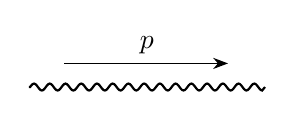
\begin{tikzpicture}[baseline={(0,-0.1)}]
    \begin{feynman}
        \vertex (a);
        \vertex [right=3cm of a] (b);
        \diagram* {
            (a) -- [photon, momentum=\(p\), thick] (b)
        };
    \end{feynman}
\end{tikzpicture}}
= \frac{-i}{p^{2}+i\epsilon}\left[g_{\mu\nu}-(1-\xi)\frac{p_{\mu}p_{\nu}}{p^{2}}\right].
\end{equation}

For most cases, we will use the Feynman Gauge, $\xi=1$, unless we are checking the gauge invariance explicitly. The photon propagator under the Feynman gauge is
\begin{equation}
{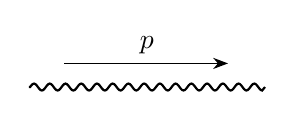
\begin{tikzpicture}[baseline={(0,-0.1)}]
    \begin{feynman}
        \vertex (a);
        \vertex [right=3cm of a] (b);
        \diagram* {
            (a) -- [photon, momentum=\(p\), thick] (b)
        };
    \end{feynman}
\end{tikzpicture}}
= \frac{-ig_{\mu\nu}}{p^{2}+i\epsilon}\quad\text{(Feynman gauge)}.
\end{equation}

A spinor propagator is represented by a solid line with an arrow pointing in the direction of particle flow (to the right for particles, left for antiparticles):
\begin{equation}
{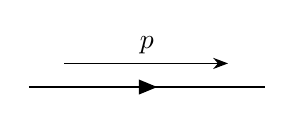
\begin{tikzpicture}[baseline={(0,-0.1)}]
    \begin{feynman}
        \vertex (a);
        \vertex [right=3cm of a] (b);
        \diagram* {
            (a) -- [fermion, momentum=\(p\), thick] (b)
        };
    \end{feynman}
\end{tikzpicture}}
= \frac{i(\slashed{p}+m)}{p^{2}-m^{2}+i\epsilon}.
\end{equation}

Just as in scalar QED, external photon lines get polarization vectors:
\begin{equation}
{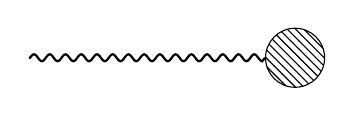
\begin{tikzpicture}[baseline={(0,-0.1)}]
    \begin{feynman}
        \vertex (a);
        \vertex [right=3cm of a, blob] (b) {};
        \diagram* {
            (a) -- [photon, thick] (b)
        };
    \end{feynman}
\end{tikzpicture}}
= \epsilon_{\mu}(p)\quad\text{(incoming)},
\end{equation}

\begin{equation}
{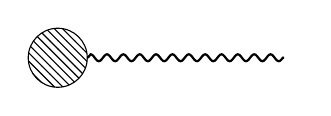
\begin{tikzpicture}[baseline={(0,-0.1)}]
    \begin{feynman}
        \vertex [blob] (a) {};
        \vertex [right=3cm of a] (b) {};
        \diagram* {
            (b) -- [photon, thick] (a)
        };
    \end{feynman}
\end{tikzpicture}}
= \epsilon^{*}_{\mu}(p)\quad\text{(outgoing)}.
\end{equation}

Similarly, external fermions get spinors, with $u$ spinors for electrons and $v$spinors for positrons:
\begin{equation}
{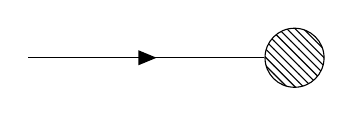
\begin{tikzpicture}[baseline={(0,-0.1)}]
    \begin{feynman}
        \vertex (a);
        \vertex [right=3cm of a, blob] (b) {};
        \diagram* {
            (a) -- [fermion] (b)
        };
    \end{feynman}
\end{tikzpicture}}
= u^{s}(p),
\end{equation}

\begin{equation}
{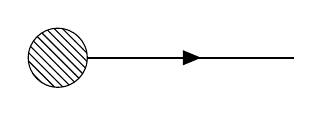
\begin{tikzpicture}[baseline={(0,-0.1)}]
    \begin{feynman}
        \vertex [blob] (a) {};
        \vertex [right=3cm of a] (b);
        \diagram* {
            (a) -- [fermion, thick] (b)
        };
    \end{feynman}
\end{tikzpicture}}
= \bar{u}^{s}(p),
\end{equation}

\begin{equation}
{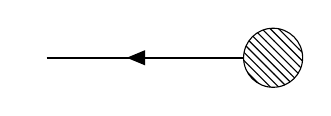
\begin{tikzpicture}[baseline={(0,-0.1)}]
    \begin{feynman}
        \vertex (a) {};
        \vertex [right=3cm of a, blob] (b) {};
        \diagram* {
            (a) -- [anti fermion, thick] (b)
        };
    \end{feynman}
\end{tikzpicture}}
= \bar{v}^{s}(p),
\end{equation}

\begin{equation}
{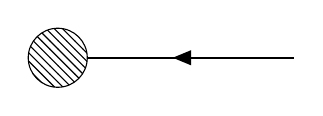
\begin{tikzpicture}[baseline={(0,-0.1)}]
    \begin{feynman}
        \vertex [blob] (a) {};
        \vertex [right=3cm of a] (b);
        \diagram* {
            (a) -- [anti fermion, thick] (b)
        };
    \end{feynman}
\end{tikzpicture}}
= v^{s}(p).
\end{equation}
The external spinors are forced to be on-shell by the LSZ reduction formula. Thus, we can use the equations of motion to simplify the calculations:
\begin{equation}
(\slashed{p}-m)u^{s}(p) = \bar{u}^{s}(p)(\slashed{p}-m)=0,
\end{equation}
\begin{equation}
(\slashed{p}+m)v^{s}(p) = \bar{v}^{s}(p)(\slashed{p}+m)=0.
\end{equation}

Now, we shall investigate the interactions for QED. By expanding the Lagrangian, we find 
\begin{equation}
    \mathcal{L}_\text{int} = -e\bar{\psi}\gamma^\mu A_\mu \psi.
\end{equation}
Note, unlike scalar QED, there is no derivative, and thus no factor of momentum.
% Case 1: Electron-photon vertex (incoming electron, outgoing electron, incoming photon)
\begin{equation}
\raisebox{0.1\height}{
\begin{tikzpicture}[baseline={(0,0)}]
    \begin{feynman}
        \vertex (a);
        \vertex [right=1.5cm of a] (b);
        \vertex [above right=1.5cm of b] (c);
        \vertex [below right=1.5cm of b] (d);
        \diagram* {
            (a) -- [fermion] (b),
            (b) -- [photon] (c),
            (b) -- [fermion] (d),
        };
    \end{feynman}
\end{tikzpicture}
}
= -ie\gamma^{\mu},
\end{equation}

% Case 2: Positron-photon vertex (incoming positron, outgoing positron, incoming photon)
\begin{equation}
\raisebox{0.1\height}{
\begin{tikzpicture}[baseline={(0,0)}]
    \begin{feynman}
        \vertex (a);
        \vertex [right=1.5cm of a] (b);
        \vertex [above right=1.5cm of b] (c);
        \vertex [below right=1.5cm of b] (d);
        \diagram* {
            (a) -- [anti fermion] (b),
            (b) -- [photon] (c),
            (b) -- [anti fermion] (d),
        };
    \end{feynman}
\end{tikzpicture}
}
= -ie\gamma^{\mu},
\end{equation}

% Case 3: Electron-positron annihilation (incoming electron, incoming positron, outgoing photon)
\begin{equation}
\raisebox{0.1\height}{
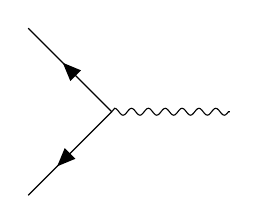
\begin{tikzpicture}[baseline={(0,0)}]
    \begin{feynman}
        \vertex (a);
        \vertex [left=1.5cm of a] (b);
        \vertex [above left=1.5cm of b] (c);
        \vertex [below left=1.5cm of b] (d);
        \diagram* {
            (a) -- [photon] (b),      % Incoming electron
            (d) -- [anti fermion] (b), % Incoming positron
            (b) -- [fermion] (c),       % Outgoing photon
        };
    \end{feynman}
\end{tikzpicture}
}
= -ie\gamma^{\mu},
\end{equation}

% Case 4: Pair production (incoming photon, outgoing electron, outgoing positron)
\begin{equation}
\raisebox{0.1\height}{
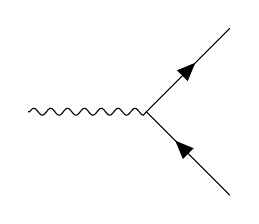
\begin{tikzpicture}[baseline={(0,0)}]
    \begin{feynman}
        \vertex (a);
        \vertex [right=1.5cm of a] (b);
        \vertex [above right=1.5cm of b] (c);
        \vertex [below right=1.5cm of b] (d);
        \diagram* {
            (a) -- [photon] (b),       % Incoming photon
            (b) -- [fermion] (c),      % Outgoing electron
            (b) -- [anti fermion] (d), % Outgoing positron
        };
    \end{feynman}
\end{tikzpicture}
}
= -ie\gamma^{\mu}.
\end{equation}

The $\mu$ on the $\gamma^\mu$ will be contracted with the $\mu$ of the photon, which would either be the $\epsilon_\mu$ of a polarization vector or the $g_{\mu\nu}$ of the photon propagator.

If there is an internal fermion line between ends, the fermion propagator should go between the end spinors:
\begin{equation}
{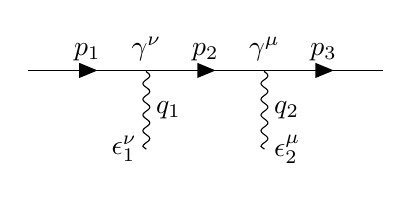
\begin{tikzpicture}[baseline={(-4,-0.1)}]
    \begin{feynman}
        \vertex (a);
        \vertex [right=1.5cm of a, label=$\gamma^\nu$] (b);
        \vertex [right=1.5cm of b, label=$\gamma^\mu$] (i);
        \vertex [right=1.5cm of i] (c);
        \vertex [below=1cm of b] (d);
        \vertex [below=1cm of i] (e);
        \diagram* {
            (a) -- [fermion, edge label=\(p_1\)] (b),
            (b) -- [fermion, edge label=\(p_2\)] (i),
            (i) -- [fermion, edge label=\(p_3\)] (c),
            (b) -- [photon, edge label=\(q_1\)] (d),
            (i) -- [photon, edge label=\(q_2\)] (e),
        };
        \node[left] at (d) {\(\epsilon^\nu_1\)};
        \node[right] at (e) {\(\epsilon^\mu_2\)};
    \end{feynman}
\end{tikzpicture}}
= (-ie)^{2}\bar{u}(p_{3})\gamma^{\mu} \frac{i(\slashed{p}_{2}+m)}{p_{2}^{2}-m^{2}+i\epsilon}\gamma^{\nu}u(p_{1})\epsilon^{2}_{\mu}(q_{2})\,\epsilon^{1}_{\nu}(q_{1}),
\end{equation}
where, by momentum conservation, $q_1 = p_1 - p_2$ and $q_2 = p_2-p_3$. Putting the spinor indices back, we get
\begin{equation}
\bar{u}(p_{3})\gamma^{\mu}\frac{i(\slashed{p}_{2}+m)}{p_{2}^{2}-m^{2}+i\epsilon}\gamma^{\nu}u(p_{1}) = \bar{u}_{\alpha}(p_{3})\,\gamma^{\mu}_{\alpha\beta}\frac{i(\slashed{p}_{2}+m)_{\beta\gamma}}{p_{2}^{2}-m^{2}+i\epsilon}\gamma^{\nu}_{\gamma\delta}u_{\delta}(p_{1}).
\end{equation}
If we tie the ends of the diagram together, we would get a loop. Thus, we must replace the $u_\delta\bar{u}_\alpha$ by a propagator, which sums over all possible spins. We should also integrate over all momenta constrained by momentum conservation at each vertex. So the loop becomes
\begin{equation}
\begin{aligned}
i\mathcal{M}&
={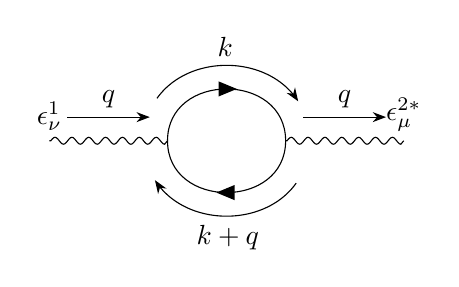
\begin{tikzpicture}[baseline={(-2,-0.1)}]
    \begin{feynman}
        \vertex (a);
        \vertex [right=1.5cm of a] (b);
        \vertex [right=1.5cm of b] (c);
        \vertex [right=1.5cm of c] (d);
        \diagram* {
            (a) -- [photon, momentum=\(q\)] (b),
            (b) -- [fermion, half left, momentum=\(k\)] (c),
            (c) -- [fermion, half left, momentum=\(k+q\)] (b),
            (c) -- [photon, momentum=\(q\)] (d),
        };
        \node[above] at (a) {\(\epsilon_\nu^1\)};
        \node[above] at (d) {\(\epsilon_\mu^{2*}\)};
    \end{feynman}
\end{tikzpicture}}\\
&= -(-ie)^2 \int \frac{d^4k}{(2\pi)^4} e^{2*}_\mu (q) e^{1}_\nu (q) \left[ \gamma^\mu_{\alpha\beta} \frac{i(\slashed{k} + \slashed{q} + m)_{\beta\gamma}}{(k+q)^2 - m^2 + i\epsilon} \gamma^\nu_{\gamma\delta} \frac{i(\slashed{k} + m)_{\delta\alpha}}{k^2 - m^2 + i\epsilon} \right]\\
&= e^2\epsilon_\mu^{2*}\epsilon_\nu^1\int \frac{d^4 k}{(2\pi)^4}\text{Tr}\left[\gamma^{\mu}\frac{i(\slashed{k}+\slashed{q}+m)}{(k+q)^2-m^2+i\epsilon}\gamma^{\nu}\frac{i(\slashed{k}+m)}{(k^2-m^2+i\epsilon)}\right].
\end{aligned}
\end{equation}
A useful general rule is that the spinor matrices are always multiplied together in the direction opposite to the particle-flow arrow.

\subsubsection{Signs}
Now, the subtlety comes in. Recall that the spinors anticommute within a time-ordered product:
\begin{equation}
    T\{\cdots \psi(x)\psi(y) \cdots \} = - T\{\cdots \psi(y)\psi(x) \cdots \}.
\end{equation}
These minus signs would also appear in the Feynman rules. To see it, let us consider the Møller scattering ($e^-e^-\to e^-e^-$) at tree-level. Two possible Feynman diagrams contribute at tree-level, the $t$-channel diagram:
% t-channel Møller scattering
\begin{equation}
i\mathcal{M}_{t} = 
\raisebox{-1.5cm}{
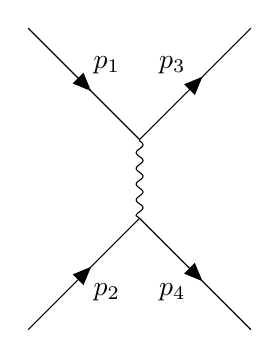
\begin{tikzpicture}[baseline={(0,-3.5cm)}]
    \begin{feynman}
        \vertex (i1);
        \vertex [below right=2cm of i1] (a);
        \vertex [above right=2cm of a] (f1);
        \vertex [below=1cm of a] (b);
        \vertex [below right=2cm of b] (f2);
        \vertex [below left=2cm of b] (i2);

        \diagram* {
        (i1) --[fermion, edge label = \(p_1\)] (a),
        (i2) --[fermion, edge label' = \(p_2\)] (b),
        (a) --[photon] (b),
        (a) --[fermion, edge label = \(p_3\)] (f1),
        (b) -- [fermion, edge label' = \(p_4\)](f2),
        };
    \end{feynman}
\end{tikzpicture}}
= \pm(-ie)^2 \bar{u}(p_3)\gamma^\mu u(p_1)\frac{-ig_{\mu\nu}}{(p_1-p_3)^2}\bar{u}(p_4)\gamma^\nu u(p_2)
\end{equation}

\begin{equation}
i\mathcal{M}_{u} = 
\raisebox{-1.5cm}{
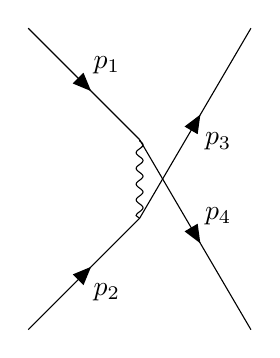
\begin{tikzpicture}[baseline={(0,-3.5cm)}]
    \begin{feynman}
        \vertex (i1);
        \vertex [below right=2cm of i1] (a);
        \vertex [above right=2cm of a] (f1);
        \vertex [below=1cm of a] (b);
        \vertex [below right=2cm of b] (f2);
        \vertex [below left=2cm of b] (i2);

        \diagram* {
        (i1) --[fermion, edge label = \(p_1\)] (a),
        (i2) --[fermion, edge label' = \(p_2\)] (b),
        (a) --[photon] (b),
        (a) --[fermion, edge label = \(p_4\)] (f2),
        (b) -- [fermion, edge label' = \(p_3\)](f1),
        };
    \end{feynman}
\end{tikzpicture}}
= \pm(-ie)^2 \bar{u}(p_4)\gamma^\mu u(p_2)\frac{-ig_{\mu\nu}}{(p_1-p_4)^2}\bar{u}(p_4)\gamma^\nu u(p_1)
\end{equation}
What sign does these diagrams give?

The sum of amplitudes of these two diagrams is given by the perturbation expansion at order $e^2$:
\begin{equation}
\begin{aligned}
&(-ie)^{2}\int d^{4}x\int d^{4}y\langle 0|T\left\{\psi(x_{1})\bar{\psi}(x_{3})\psi(x_{2})\bar{\psi}(x_{4})\Big{(}\bar{\psi}(x)A(x)\psi(x)\Big{)}\Big{(}\bar{\psi}(y)A(y)\psi(y)\Big{)}\right\}|0\rangle\\
&=(-ie)^{2}\gamma^{\mu}_{\beta_{1}\beta_{2}}\gamma^{\nu}_{\beta_{3}\beta_{4}}\int d^{4}x\int d^{4}y
\langle 0|T\Big{\{}\psi_{\alpha_{1}}(x_{1})\bar{\psi}_{\alpha_{3}}(x_{3})\psi_{\alpha_{2}}(x_{2})\bar{\psi}_{\alpha_{4}}(x_{4})\bar{\psi}_{\beta_{1}}(x)\\
& \qquad \qquad \qquad \qquad \qquad \qquad \qquad \qquad \qquad \qquad  \times A^{\mu}(x)\psi_{\beta_{2}}(x)\bar{\psi}_{\beta_{3}}(y)A^{\nu}(y)\psi_{\beta_{4}}(y)\Big{\}}|0\rangle.
\end{aligned}
\end{equation}
Recall Wick's theorem, which states that the vacuum matrix element of a time-ordered product is equal to all possible contractions in which all the fields are involved. For scalar field theory, a contraction is just a Feynman propagator:
\begin{equation}
    \wick{\c\phi(x_1)\c\phi(x_2)} = \bra{0}T\{\phi(x_1)\phi(x_2)\}\ket{0}.
\end{equation}
The same thing also applies to spinors. Thus, the vacuum matrix element of a time-ordered product is equal to all combinations of Feynman propagators in which all the spinors are involved. Since the Feynman propagator of spinors anticommutes, we must first put them in the correct order and then contract them. 


 For the above expansion, there are two possible contractions corresponding to the $t$- and $u$-channel. For the $t$-channel, the top electron line is created by $\bar{\psi}(x_3)$ annihilated by $\psi(x)$, created by $\bar{\psi}(x)$ annihilated by $\psi(x_1)$, and similarly for the bottom line. So we have
\begin{equation}
\begin{aligned}
&(-ie)^{2}\gamma^{\mu}_{\beta_{1}\beta_{2}}\gamma^{\nu}_{\beta_{3}\beta_{4}}\int d^{4}x\int d^{4}y \\
& \times\langle 0|T\{A^{\mu}(x)A^{\nu}(y)\psi_{\alpha_{1}}(x_{1})\psi_{\beta_{1}}(x)\psi_{\beta_{2}}(x)\bar{\psi}_{\alpha_{3}}(x_{3})\psi_{\alpha_{2}}(x_{2})\bar{\psi}_{\beta_{3}}(y)\psi_{\beta_{4}}(y)\bar{\psi}_{\alpha_{4}}(x_{4})\}|0\rangle.
\end{aligned}
\end{equation}
For $u$-channel, however, we need to swap $\bar{\psi}(x_3)$ and $\bar{\psi}(x_4)$, which gives an extra negative sign:
\begin{equation}
\begin{aligned}
&-(-ie)^{2}\gamma^{\mu}_{\beta_{1}\beta_{2}}\gamma^{\nu}_{\beta_{3}\beta_{4}}\int d^{4}x\int d^{4}y \\
& \times\langle 0|T\{A^{\mu}(x)A^{\nu}(y)\psi_{\alpha_{1}}(x_{1})\psi_{\beta_{1}}(x)\psi_{\beta_{2}}(x)\bar{\psi}_{\alpha_{4}}(x_{4})\psi_{\alpha_{2}}(x_{2})\bar{\psi}_{\beta_{3}}(y)\psi_{\beta_{4}}(y)\bar{\psi}_{\alpha_{3}}(x_{3})\}|0\rangle.
\end{aligned}
\end{equation}
Thus the matrix element of Møller scattering at tree-level has the form
\begin{equation}
    \mathcal{M} = \mathcal{M}_t + \mathcal{M}_u = e^2\bigg\{ \frac{[\bar{u}(p_3)\gamma^\mu u(p_1)][\bar{u}(p_4)\gamma^\mu u(p_2)]}{(p_1-p_3)^2} - \frac{[\bar{u}(p_4)\gamma^\mu u(p_1)][\bar{u}(p_3)\gamma^\mu u(p_2)]}{(p_1-p_4)^2} \bigg\}.
\end{equation}
In the above, we have assumed the $t$-channel to be positive, but we could also have chosen the $u$-channel to be positive. However, the only physical quantity is $\abs{\mathcal{M}}^2$. Thus, only the difference in sign would matter.

Now, consider a loop such as
\begin{equation}
{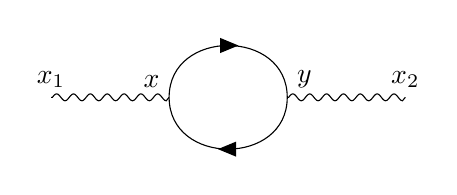
\begin{tikzpicture}[baseline={(0,0)}]
    \begin{feynman}
        \vertex (a);
        \vertex [right=1.5cm of a] (b);
        \vertex [right=1.5cm of b] (c);
        \vertex [right=1.5cm of c] (d);
        \diagram* {
            (a) -- [photon] (b),
            (b) -- [fermion, half left] (c),
            (c) -- [fermion, half left] (b),
            (c) -- [photon] (d),
        };
        \node[above] at (a) {\(x_1\)};
        \node[above] at (d) {\(x_2\)};
        \node[above left] at (b) {$x$};
        \node[above right] at (c) {$y$};
    \end{feynman}
\end{tikzpicture}}
\end{equation}
which comes from the expansion
\begin{equation}
    (-ie)^2\gamma^\mu\gamma^\nu\gamma^\alpha\gamma^\beta\int d^4x \int d^4y \bra{0}T\{ A^\mu(x_1) A^\nu(x_2)\bar{\psi}(x)A^\alpha(x)\psi(x)\bar{\psi}(y)A^\beta(y)\psi(y) \}\ket{0}.
\end{equation}
To get the spinors into the order such that they are created then immediately destroyed, we need to anticommute $\psi(y)$ from the right to the left. That is, we use

\[
\bar{\psi}_{\alpha}(x)\psi_{\beta}(x)\bar{\psi}_{\gamma}(y)\psi_{\delta}(y)=- \psi_{\delta}(y)\bar{\psi}_{\alpha}(x)\psi_{\beta}(x)\bar{\psi}_{\gamma}(y).
\]

Thus, the Feynman rule for this fermion loop should be supplemented with an additional minus sign. As an exercise, you should check that adding more photons to a fermionic loop does not change this overall minus sign.

In summary, the Feynman rules for fermions must be supplemented by a factor of
\begin{shaded}
\begin{itemize}
    \item \(-1\) for interchange of external identical fermions. Diagrams such as \(s\)- and \(t\)-channel exchanges, which would be present even for non-identical particles, do not get an extra minus sign. The \(-1\) is a relative minus sign between two diagrams that are related by interchanging two external identical particles.
    \item \(-1\) for each fermion loop.
\end{itemize}
\end{shaded}

\subsection{$\gamma$-matrix Identities}
Before doing any QED calculations, let us first derive some useful identities. We will often be dealing with traces of products of $\gamma$-matrices. These can often be simplified using the cyclic propety of traces:
\begin{equation}
    \Tr[AB\cdots C] = \Tr[B \cdots CA].
\end{equation}

Another useful thing to note is that
\begin{equation}
    \gamma_5^2 = 1, \quad \gamma_5\gamma_\mu = -\gamma_\mu\gamma_5.
\end{equation}

First, compute
\begin{equation}
    \Tr[g^{\mu\nu}] = \Tr[g^{\mu\nu}\mathds{1}] + g^{\mu\nu}\Tr[\mathds{1}] = 4g^{\mu\nu},
\end{equation}
where we have used $\mathds{1}$ to denote the identity matrix of the spinor indices.

Next, we evaluate
\begin{equation}
    \Tr[\gamma^\mu] = \Tr[\gamma^5\gamma^5\gamma^\mu] = -Tr[\gamma^5\gamma^\mu\gamma^5]  = -\Tr[\gamma^5\gamma^5\gamma^\mu] = -\Tr[\gamma^\mu] \implies \Tr[\gamma^\mu] = 0.
\end{equation}

Then for the trace of a product of two $\gamma$-matrices, we find
\begin{equation}
    \Tr[\gamma^\mu\gamma^\nu] = \Tr[2g^{\mu\nu}-\gamma^\nu\gamma^\mu] = 8g^{\mu\nu} -\Tr[\gamma^\mu\gamma^\nu] \implies \Tr[\gamma^\mu\gamma^\nu] = 4g^{\mu\nu}.
\end{equation}

For three $\gamma$-matrices, we have
\begin{equation}
    \Tr[\gamma^\mu\gamma^\nu\gamma^\alpha] = \Tr[\gamma^5\gamma^5\gamma^\mu\gamma^\nu\gamma^\alpha] = -\Tr [\gamma^5\gamma^\mu\gamma^\nu\gamma^\alpha\gamma^5] =  -\Tr[\gamma^\mu\gamma^\nu\gamma^\alpha] \implies \Tr[\gamma^\mu\gamma^\nu\gamma^\alpha] = 0.
\end{equation}
Since we can always do the same thing for traces of odd number of $\gamma$-matrices, they must be zero.

Now, for four $\gamma$-matrices, we find
\begin{equation}
\begin{aligned}
        \Tr[\gamma^\alpha\gamma^\mu\gamma^\beta\gamma^\nu] &= \Tr[(2g^{\alpha\mu}-\gamma^\mu\gamma^\alpha)\gamma^\beta\gamma^\nu] \\
        &= 2g^{\alpha\mu}\Tr[\gamma^\beta\gamma^\nu] - \Tr[\gamma^\mu\gamma^\alpha\gamma^\beta\gamma^\nu]\\
        &= 8g^{\alpha\mu}g^{\beta\nu} - 2g^{\alpha\beta}\Tr[\gamma^\mu\gamma^\nu] +\Tr[\gamma^\mu\gamma^\beta\gamma^\alpha\gamma^\nu] \\
        &= 8g^{\alpha\mu}g^{\beta\nu} - 8g^{\alpha\beta}g^{\mu\nu} +2g^{\alpha\nu}\Tr[\gamma^\mu\gamma^\beta] - \Tr[\gamma^\mu\gamma^\beta\gamma^\nu\gamma^\alpha]\\
        &=  8g^{\alpha\mu}g^{\beta\nu} - 8g^{\alpha\beta}g^{\mu\nu} +8g^{\alpha\nu}g^{\beta\mu} -\Tr[\gamma^\alpha\gamma^\mu\gamma^\beta\gamma^\nu]\\
        &\implies \Tr[\gamma^\alpha\gamma^\mu\gamma^\beta\gamma^\nu] = 4(g^{\alpha\mu}g^{\beta\nu} - g^{\alpha\beta}g^{\mu\nu} +g^{\alpha\nu}g^{\beta\mu}).
\end{aligned}
\end{equation}
Such method can be trivially applied to traces with more $\gamma$-matrices.

\subsection{$e^+e^-\to \mu^+\mu^-$}
As far as the QED is concerned, the muon, $\mu^-$, is a particle identical to the electron, except heavier. $e^+e^-\to\mu^+\mu^-$, is the simplest tree-level scattering process in QED. We will calculate at tree-level here and give the 1-loop correction later. The leading order contribution is
\begin{equation}
    \begin{aligned}
        i\mathcal{M}
        &={
        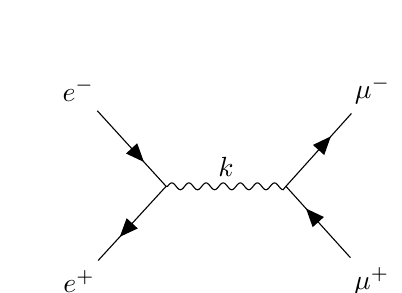
\begin{tikzpicture}[baseline={(0,0.5)}]
        \feynmandiagram [horizontal=a to b] {
        i1 [particle=\(e^{+}\)] -- [anti fermion] a -- [anti fermion] i2 [particle=\(e^{-}\)],
        a -- [photon, edge label=\(k\)] b,
        f1 [particle=\(\mu^{-}\)] -- [anti fermion] b -- [anti fermion] f2 [particle=\(\mu^{+}\)],
        };            
        \end{tikzpicture}}\\
        \\
        &= (-ie)\bar{v}_\alpha(p_2)\gamma^\mu_{\alpha\beta}u_\beta(p_1) \frac{-i\left[g_{\mu\nu} - (1-\xi)\frac{k_\mu k_\nu}{k^2} \right]}{k^2}(-ie)\bar{u}_\delta(p_3)\gamma^\nu_{\delta\tau}v_\tau(p_4),
        \label{EQ. eemm}
    \end{aligned}
\end{equation}
where $k^\mu = p_1^\mu + p_2^\mu = p_3^\mu + p_4^\mu$. The external spinors are forced to be on-shell, thus we can use the equations of motion $\slashed{p}_1u(p_1)=mu(p_1)$ and $\bar{v}(p)_2\slashed{p_2} = -m\bar{v}(p_2)$. Thus, 
\begin{equation}
    \begin{aligned}
        \bar{v}_\alpha(p_2)\gamma^\mu_{\alpha\beta}u_\beta(p_1)k_\mu &= \bar{v}(p_2)\slashed{p}_1u(p_1) + \bar{v}(p_2)\slashed{p}_2u(p_1) \\
        &= \bar{v}(p_2)mu(p_1) - \bar{v}(p_2)mu(p_1)  = 0.
    \end{aligned}
\end{equation}
Similarly, for the other term contracted with $k^\nu$. Thus, the $k^\mu k^\nu$ term vanishes, which is expected by gauge invariance. Hence, (\ref{EQ. eemm}) becomes
\begin{equation}
    \mathcal{M} = \frac{e^2}{s}[\bar{v}(p_2)\gamma^\mu u(p_1)][\bar{u}(p_3)\gamma^\mu v(p_4)].
    \label{EQ. M eemm}
\end{equation}

Now, we need to find the conjugate amplitude to calculate $\abs{\mathcal{M}}^2$. Using $\gamma^{0\dagger} = \gamma^0$ and $\gamma^{\mu^\dagger}\gamma^0 = \gamma^0 \gamma^\mu$, we find
\begin{equation}
    (\bar{\psi}_1\gamma^\mu\psi_2)^\dagger = \psi_2^\dagger\gamma^{\mu\dagger}\gamma^0\psi_1 = \psi_2^\dagger\gamma^0\gamma^{\mu}\psi_1 = \bar{\psi}_2 \gamma^\mu \psi_1,
\end{equation}

Hence, the conjugate of (\ref{EQ. M eemm}) is given by
\begin{equation}
    \mathcal{M}^\dagger = \frac{e^2}{s}[\bar{v}(p_4)\gamma^\mu u(p_3)][\bar{u}(p_1)\gamma^\mu v(p_2)],
\end{equation}
and thus
\begin{equation}
    \abs{\mathcal{M}}^2 = \frac{e^4}{s^2}[\bar{v}(p_2)\gamma^\mu u(p_1)][\bar{u}(p_3)\gamma^\mu v(p_4)][\bar{v}(p_4)\gamma^\nu u(p_3)][\bar{u}(p_1)\gamma^\nu v(p_2)].
\end{equation}

\subsubsection{Unpolarized Scattering}
The easiest thing to calculate from this is the cross section for scattering, assuming the spin is not measured. Then the final cross section should be the sum of all possible spin outcomes, which is
\begin{equation}
\begin{aligned}
        \sum_{s,s'}\abs{\mathcal{M}}^2 &= \sum_{s,s'}\frac{e^4}{s^2}[\bar{v}^r(p_2)\gamma^\mu u^{r'}(p_1)][\bar{u}^{r'}(p_1)\gamma^\nu v^r(p_2)][\bar{u}^s(p_3)\gamma^\mu v^{s'}(p_4)][\bar{v}^{s'}(p_4)\gamma^\nu u^s(p_3)] \\
        &= \frac{e^4}{s^2}[\bar{v}^r(p_2)\gamma^\mu u^{r'}(p_1)][\bar{u}^{r'}(p_1)\gamma^\nu v^r(p_2)]\sum_{s,s'}[\bar{u}_\alpha^s(p_3)\gamma^\mu_{\alpha\beta} v^{s'}_\beta(p_4)\bar{v}_\gamma^{s'}(p_4)\gamma^\nu_{\gamma\delta} u^s_\delta(p_3)] \\
        &= \frac{e^4}{s^2}[\bar{v}^r(p_2)\gamma^\mu u^{r'}(p_1)][\bar{u}^{r'}(p_1)\gamma^\nu v^r(p_2)]\sum_{s}[\bar{u}_\alpha^s(p_3)\gamma^\mu_{\alpha\beta} (\slashed{p}_4-m_\mu)_{\beta\gamma}\gamma^\nu_{\gamma\delta} u^s_\delta(p_3)] \\
        &= \frac{e^4}{s^2}[\bar{v}^r(p_2)\gamma^\mu u^{r'}(p_1)][\bar{u}^{r'}(p_1)\gamma^\nu v^r(p_2)][(\slashed{p}_3+m_\mu)_{\delta\alpha}\gamma^\mu_{\alpha\beta} (\slashed{p}_4-m_\mu)_{\beta\gamma}\gamma^\nu_{\gamma\delta}] \\
        &= \frac{e^4}{s^2}[\bar{v}^r(p_2)\gamma^\mu u^{r'}(p_1)][\bar{u}^{r'}(p_1)\gamma^\nu v^r(p_2)]\Tr[(\slashed{p}_3+m_\mu)\gamma^\mu (\slashed{p}_4-m_\mu)\gamma^\nu],
\end{aligned}
\end{equation}
where we have used
\begin{equation}
    \sum_s u_\alpha(p)\bar{u}_\beta(p) = \sum_s \bar{u}_\beta(p)u_\alpha(p) = (\slashed{p}+m)_{\alpha\beta}.
\end{equation}

We shall also assume that we do not know the spins of the initial states. If we do the measurements for many times, we would get the average over each spin. Therefore, we shall take the average of the initial spins, which is
\begin{equation}
    \begin{aligned}
        \frac{1}{4}\sum_{r,r'}\sum_{s,s'}\abs{\mathcal{M}}^2 &= \frac{1}{4}\sum_\text{spins}\abs{\mathcal{M}}^2\\
        &= \frac{e^4}{4s^2}\Tr[(\slashed{p}_1 + m_e)\gamma^\nu(\slashed{p}_2-m_e)\gamma^\mu]\Tr[(\slashed{p}_3+m_\mu)\gamma^\mu (\slashed{p}_4-m_\mu)\gamma^\nu].
        \label{EQ. M eemm3}
    \end{aligned}
\end{equation}
The trace can be simplified as
\begin{equation}
    \begin{aligned}
        \Tr[(\slashed{p}_3+m_\mu)\gamma^\mu (\slashed{p}_4-m_\mu)\gamma^\nu] &= p_3^\alpha p_4^\beta\Tr[\gamma^\alpha\gamma^\mu\gamma^\beta\gamma^\nu] - m_\mu^2\Tr[\gamma^\mu\gamma^\nu] \\
        &= 4p_3^\alpha p_4^\beta(g^{\alpha\mu}g^{\beta\nu} - g^{\alpha\beta}g^{\mu\nu} +g^{\alpha\nu}g^{\beta\mu}) - 4m_\mu^2g^{\mu\nu}\\
        &= 4p_3^\mu p_4^\nu - 4p_{34}g^{\mu\nu} + 4p_3^\nu p_4^\mu - 4m_\mu^2g^{\mu\nu}
    \end{aligned}
\end{equation}
with $p_{ij} \equiv p_i \cdot p_j$. Thus,
\begin{equation}
    \begin{aligned}
        \frac{1}{4}\sum_\text{spins}\abs{\mathcal{M}}^2 &= \frac{e^4}{4s^2}[4p_1^\mu p_2^\nu - 4p_{12}g^{\mu\nu} + 4p_1^\nu p_2^\mu - 4m_e^2g^{\mu\nu}
        ][4p_3^\mu p_4^\nu - 4p_{34}g^{\mu\nu} + 4p_3^\nu p_4^\mu - 4m_\mu^2g^{\mu\nu}] \\
        &= \frac{e^4}{4s^2}[4p_1^\mu p_2^\nu + 4p_1^\nu p_2^\mu - 4(p_{12} +m_e^2)g^{\mu\nu}
        ][4p_3^\mu p_4^\nu  + 4p_3^\nu p_4^\mu - 4(p_{34} + m_\mu^2)g^{\mu\nu}]\\
        &= \frac{4e^4}{s^2}[2p_{13}p_{24} + 2p_{14}p_{23} + 4(p_{12} +m_e^2)(p_{34} + m_\mu^2) - 2(p_{12} +m_e^2)p_{34} - 2(p_{34} + m_\mu^2)p_{12}] \\
        &= \frac{8e^4}{s^2}(p_{13}p_{24} + p_{14}p_{23} + p_{12}m_\mu^2 + p_{34}m_e^2 + 2m_\mu^2m_e^2).
    \end{aligned}
\end{equation}
This can be written in terms of the Mandelstam variables:
\begin{equation}
    \begin{aligned}
        s &= (p_{1} + p_{2})^{2} = (p_{3} + p_{4})^{2} = 2m_{e}^{2} + 2p_{12} = 2m_{\mu}^{2} + 2p_{34}, \\
        t &= (p_{1} - p_{3})^{2} = (p_{2} - p_{4})^{2} = m_{e}^{2} + m_{\mu}^{2} - 2p_{13} = m_{e}^{2} + m_{\mu}^{2} - 2p_{24}, \\
        u &= (p_{1} - p_{4})^{2} = (p_{2} - p_{3})^{2} = m_{e}^{2} + m_{\mu}^{2} - 2p_{14} = m_{e}^{2} + m_{\mu}^{2} - 2p_{23}. \\
    \end{aligned}   
\end{equation}

Plugging these in, we have
\begin{equation}
    \begin{aligned}
        \frac{1}{4}\sum_\text{spins}\abs{\mathcal{M}}^2 &= \frac{8e^4}{s^2}\bigg[ \left(\frac{m_e^2+m_\mu^2-t}{2}\right)^2 + \left(\frac{m_e^2+m_\mu^2-u}{2}\right)^2 \\
        &\qquad \qquad \qquad \qquad+ \left(\frac{s-2m_e^2}{2}\right)m_\mu^2 + \left(\frac{s-2m_\mu^2}{2}\right)m_e^2 + 2m_\mu^2m_e^2\bigg] \\
        &= \frac{2e^4}{s^2}\bigg[ 2m_e^4 + 2m_\mu^4 + 4m_e^2m_\mu^2 -2t(m_e^2+m_\mu^2) -2u(m_e^2+m_\mu^2) \\
        &\qquad \qquad \qquad \qquad+ t^2 + u^2 + 2s(m_e^2 + m_\mu^2) -8m_e^2m_\mu^2 + 8m_e^2m_\mu^2 \bigg] \\
        &= \frac{2e^4}{s^2}\bigg[ t^2 + u^2 + 2(s-t-u)(m_e^2+m_\mu^2) + 2m_e^4 + 2m_\mu^4 \bigg].
    \end{aligned}
\end{equation}
Also, note
\begin{equation}
    \begin{aligned}
        s+u+t &= (2m_{e}^{2} + 2p_{12}) + (m_{e}^{2} + m_{\mu}^{2} - 2p_{13}) +( m_{e}^{2} + m_{\mu}^{2} - 2p_{14}) \\
        &= 4m_e^2 + 2m_\mu^2 + 2p_1 \cdot (p_2-p_3-p_4) \\
        &= 4m_e^2 + 2m_\mu^2 - 2p_1^2 \\
        &= 2(m_e^2+m_\mu^2).
    \end{aligned}
\end{equation}
Thus, we have
\begin{shaded}
    \begin{equation}
        \frac{1}{4}\sum_\text{spins}\abs{\mathcal{M}}^2 = \frac{2e^4}{s^2}\bigg[ t^2 + u^2 + 4s(m_e^2+m_\mu^2) - 2(m_e^2+m_\mu^2)^2\bigg].
        \label{EQ. M eemm2}
    \end{equation}
\end{shaded}

\subsubsection{Differential Cross Section}
Now, let us compute the cross section in the centre of mass frame. Since the initial and final masses are different, the cross section is given by
\begin{equation}
    \frac{d\sigma}{d\Omega} = \frac{1}{64\pi^2E_{\text{CM}}^2}\frac{\abs{\vec{p_f}}}{\abs{\vec{p_i}}}\abs{\mathcal{M}}^2.
\end{equation}

In the centre of mass frame, let us define the energy of all the particles to be $E$ (by energy conservation), and define the momenta of the incoming particles to be $\vec{p}$, the momenta of the outgoing particles to be $\vec{q}$. So that
\begin{equation}
    \begin{aligned}
        &p_1^\mu = (E, \vec{p}),\\
        &p_2^\mu = (E, -\vec{p}),\\
        &p_3^\mu = (E, \vec{q}),\\
        &p_4^\mu = (E, -\vec{q}).\\
    \end{aligned}
\end{equation}
The Mandelstam variables become,
\begin{equation}
    \begin{aligned}
        s &= (p_{1} + p_{2})^{2} = 4E^2 = E_\text{CM}^2, \\
        t &= (p_{1} - p_{3})^{2} = -(\vec{p}-\vec{q})^2 = -\vec{p}^2 - \vec{q}^2 +2\vec{p}\cdot\vec{q} =  -2E^2 + m_2^2 + m_\mu^2 + 2\vec{p}\cdot\vec{q}, \\
        u &= (p_{1} - p_{4})^{2} = -(\vec{p}+\vec{q})^2 = -\vec{p}^2 - \vec{q}^2 -2\vec{p}\cdot\vec{q} = - 2E^2 + m_2^2 + m_\mu^2 -2\vec{p}\cdot\vec{q}. \\
    \end{aligned}   
\end{equation}
Thus, (\ref{EQ. M eemm2}) becomes
\begin{equation}
    \begin{aligned}
        \frac{1}{4}\sum_\text{spins}\abs{\mathcal{M}}^2 &= \frac{2e^4}{s^2}\bigg[ (2E^2 - m_2^2 - m_\mu^2 -2\vec{p}\cdot\vec{q})^2 + (2E^2 - m_2^2 - m_\mu^2 +2\vec{p}\cdot\vec{q})^2 \\
        &\qquad \qquad + 16E^2(m_e^2+m_\mu^2) - 2(m_e^2+m_\mu^2)^2\bigg] \\
        &= \frac{2e^4}{s^2}\bigg[8E^4 + 8E^2(m_e^2+m_\mu^2) + 8(\vec{p}\cdot\vec{q})^2 \bigg].
    \end{aligned}
\end{equation}
We define the angle between $\vec{p}$ and $\vec{q}$ to be $\theta$, so that
\begin{equation}
    \vec{p}\cdot\vec{q} = \abs{\vec{p}}\abs{\vec{q}}\cos\theta.
\end{equation}
The cross section then becomes
\begin{equation}
    \begin{aligned}
        \frac{d\sigma}{d\Omega} &= \frac{e^4}{4\pi^2(4E^2)^3}\frac{\abs{\vec{p}}}{\abs{\vec{q}}}\bigg[E^4 + E^2(m_e^2+m_\mu^2) + \abs{\vec{p}}^2\abs{\vec{q}}^2\cos^2\theta \bigg] \\
        &= \frac{\alpha^4}{16E^6}\frac{\sqrt{E^2-m_\mu^2}}{\sqrt{E^2-m_e^2}}\bigg[E^4 + E^2(m_e^2+m_\mu^2) + (E^2-m_e^2)(E^2-m_\mu^2)\cos^2\theta \bigg],
    \end{aligned}
\end{equation}
where $\alpha=\frac{e^2}{4\pi}$ is the fine structure constant. 

For simplicity, take $m_e=0$, we find
\begin{equation}
    \begin{aligned}
        \frac{d\sigma}{d\Omega} 
        &= \frac{\alpha^4}{16E^6}\sqrt{1-\frac{m_\mu^2}{E^2}}\bigg[E^4 + E^2m_\mu + E^2(E^2-m_\mu^2)\cos^2\theta \bigg] \\
        &= \frac{\alpha^4}{4E_\text{CM}^2}\sqrt{1-\frac{m_\mu^2}{E^2}}\bigg[\left(1+\frac{m_\mu^2}{E^2}\right) + \left(1-\frac{m_\mu^2}{E^2}\right)\cos^2\theta  \bigg].
    \end{aligned}
\end{equation}

Under the ultra-high-energy limit we can take $m_\mu=0$, which gives
\begin{shaded}
    \begin{equation}
        \frac{d\sigma}{d\Omega} = \frac{\alpha^4}{4E_\text{CM}^2}(1+\cos^2\theta).
    \end{equation}
\end{shaded}

\subsection{Rutherford Scattering $e^-p^+ \to e^-p^+$}
The classical Rutherford scattering formula is
\begin{equation}
    \frac{d\sigma}{d\Omega} = \frac{m_e^2e^4}{4p^4\sin^4\frac{\theta}{2}},
\end{equation}
where $p = \abs{\vec{p}_i} = \abs{\vec{p}_f}$ is the magnitude of the incoming electron momentum, which is the same as the magnitude of the outgoing electron.

Here, we will do the calculation in QED, while neglecting any internal structure of the proton, treating it as a point-like particle.

\subsubsection{QED Amplitude}
As far as QED is concerned, a proton and a muon are the same thing, up to a sign of the charge which gets squared anyway. Since the proton and the electron are distinguishable, the only contribution to the amplitude at tree-level is the $t$-channel:

\begin{equation}
    \begin{aligned}
        i\mathcal{M}
        ={
        \begin{tikzpicture}[baseline={(0,-1.0)}]
        \feynmandiagram [vertical=a to b] {
        i1 [particle=\(e^{-}\)] -- [fermion] a -- [fermion] f1 [particle=\(e^{-}\)],
        a -- [photon, edge label=\(k\)] b,
        f2 [particle=\(p^+\)] -- [anti fermion] b -- [anti fermion] i2 [particle=\(p^+\)],
        };            
        \end{tikzpicture}}
        = (-ie)\bar{u}(p_3)\gamma^\mu u(p_1) \frac{-i\left[g_{\mu\nu} - (1-\xi)\frac{k_\mu k_\nu}{k^2} \right]}{k^2}(ie)\bar{u}(p_4)\gamma^\nu u(p_2).
        \label{EQ. eemm}
    \end{aligned}
\end{equation}
This is almost identical to what we had before, and thus we can read off
\begin{equation}
    \abs{\mathcal{M}}^2 = \frac{e^2}{t}[\bar{u}(p_3)\gamma^\mu u(p_1)][\bar{u}(p_1)\gamma^\nu u(p_3)][\bar{u}(p_4)\gamma^\mu u(p_2)][\bar{u}(p_2)\gamma^\nu u(p_4)].
\end{equation}
Assuming we do not have any knowledge of the initial spins and do not measure the final spins, we have
\begin{equation}
    \frac{1}{4}\sum _\text{spins}\abs{\mathcal{M}}^2 = \frac{e^4}{4t^2}\Tr[(\slashed{p}_3+m_e)\gamma^\mu(\slashed{p}_1+m_e)\gamma^\nu]\Tr[(\slashed{p}_4+m_p)\gamma^\mu(\slashed{p}_2+m_p)\gamma^\nu].
\end{equation}
Comparing this with (\ref{EQ. M eemm3}), we find they are identical up to the masses after the replacement
\begin{equation}
    (p_1,p_2,p_3,p_4) \to (p_1, -p_3, p_4, -p_2).
\end{equation}
These changes send
\begin{equation}
    s = (p_1+p_2)^2 \to (p_1-p_3)^2 = t,
\end{equation}
\begin{equation}
    t = (p_1-p_3)^2 \to (p_1-p_4)^2 = u,
\end{equation}
\begin{equation}
    u = (p_1 -p_4)^2 \to (p_1+p_2)^2 = s.
\end{equation}
Thus, we find
\begin{equation}
    \frac{1}{4}\sum_\text{spins}\abs{\mathcal{M}}^2 = \frac{2e^4}{t^2}\bigg[ u^2 + s^2 + 4t(m_e^2+m_p^2) - 2(m_e^2+m_p^2)^2\bigg].
    \label{EQ. M eemm2}
\end{equation}
\subsubsection{Cross Section}
Now, let us take the $m_p \gg m_e$ limit to get the relativistic corrections to Rutherford's formula. Thus, the momenta are
\begin{equation}
    p_1^\mu = (E, \vec{p}_i), \quad p_2^\mu = (m_p,0), \quad p_3^\mu=(E, \vec{p}_f), \quad p_4^\mu=(m_p,0).
\end{equation}
The scattering angle, $\theta$, is defined as
\begin{equation}
    \vec{p}_i\cdot\vec{p}_f = p^2\cos\theta,
\end{equation}
where $p = \abs{\vec{p}_i} =\abs{\vec{p}_f}$. 

Using 
\begin{equation}
    v = \frac{p}{E} = \sqrt{1-\frac{m_e^2}{E^2}},
\end{equation}
the above becomes
\begin{equation}
    \vec{p}_i\cdot\vec{p}_f = p^2\cos\theta = v^2E^2\cos\theta.
\end{equation}

In the limit $m_p \gg m_e$ is the electron's relativistic velocity, the relevant momentum products are:
\begin{equation}
p_{13}=E^{2}(1-v^{2}\cos\theta),
\end{equation}
\begin{equation}
p_{12}=p_{23}=p_{34}=p_{14}=E m_{p},
\end{equation}
\begin{equation}
p_{24}=m_{p}^{2},
\end{equation}
where $p_{ij}\equiv p_{i}^{\mu}p_{j\mu}$ and
\begin{equation}
t=(p_{1}-p_{3})^{2}=-(\vec{p}_{i}-\vec{p}_{f})^{2}=-2p^{2}(1-\cos\theta),
\end{equation}
so that
\begin{align}
\frac{1}{4}\sum_{\text{spins}}|\mathcal{M}|^{2}
&=\frac{8e^{4}}{t^{2}}[p_{14}p_{23}+p_{12}p_{34}-m_{p}^{2}p_{13}-m_{e}^{2}p_{24}+2m_{e}^{2}m_{p}^{2}] \nonumber \\
&=\frac{8e^{4}}{4v^{4}E^{4}(1-\cos\theta)^{2}}[E^{2}m_{p}^{2}+E^{2}m_{p}^{2}v^{2}\cos\theta+m_{e}^{2}m_{p}^{2}] \nonumber \\
&=\frac{2e^{4}m_{p}^{2}}{v^{4}E^{2}(1-\cos\theta)^{2}}[2-v^{2}(1-\cos\theta)] \nonumber \\
&=\frac{e^{4}m_{p}^{2}}{v^{4}E^{2}\sin^{4}\frac{\theta}{2}}\left[1-v^{2}\sin^{2}\frac{\theta}{2}\right].
\end{align}
Thus,
\begin{shaded}
    \begin{equation}
\frac{d\sigma}{d\Omega}=\frac{e^{4}}{64\pi^{2}v^{2}p^{2}\sin^{4}\frac{\theta}{2}}\left(1-v^{2}\sin^{2}\frac{\theta}{2}\right), \qquad E\ll m_{p}.
\end{equation}
\end{shaded}
This is known as the Mott formula. Note that the limit $m_{p}\rightarrow\infty$ exists: there is no dependence on the proton mass. For slow velocities we can use $v\ll 1$ and $p\ll E\sim m_{e}$ so $v\sim\frac{p}{m_{e}}$. Thus,
\begin{equation}
\frac{d\sigma}{d\Omega}=\frac{e^{4}m_{e}^{2}}{64\pi^{2}p^{4}\sin^{4}\frac{\theta}{2}}, \qquad v\ll 1 \text{ and } E\ll m_{p}.
\end{equation}
which is the Rutherford formula. In particular, note that the normalization factors, $m_{e}^{2}$, worked out correctly.

In the very high energy limit, $E\gg m_{e}$, one can no longer assume that the final state proton is also at rest. However, one can now neglect the electron mass, so that $v=1$. Then the momenta are
\begin{equation}
p_{1}^{\mu}=(E,\vec{p}_{i}), \quad p_{2}^{\mu}=(m_{p},0), \quad p_{3}^{\mu}=(E^{\prime},\vec{p}_{f}), \quad p_{4}^{\mu}=p_{1}^{\mu}+p_{2}^{\mu}-p_{3}^{\mu}
\end{equation}
with $|\vec{p}_{i}|=E$ and $|\vec{p}_{f}|=E^{\prime}$. For $m_{e}=0$ in the proton rest frame, following the same steps as above, we find the cross section:
\begin{shaded}
    \begin{equation}
\frac{d\sigma}{d\Omega}=\frac{e^{4}}{64\pi^{2}E^{2}\sin ^{4}\frac{\theta}{2}}\frac{E^{\prime}}{E}\left(\cos ^{2}\frac{\theta}{2}+\frac{E-E^{\prime}}{m_{p}}\sin ^{2}\frac{\theta}{2}\right), \quad m_{e}\ll E.
\end{equation}
\end{shaded}
where $E^{\prime}$ is the final state electron's energy. As $m_{p}\rightarrow\infty$, $E\rightarrow E^{\prime}$ and this reduces to the $v\rightarrow 1$ limit of the Mott formula.

These formulas describe the scattering of point-like particles by other point-like particles. Note that the final forms in which we have written these cross sections depend only on properties of the initial and final electrons. Thus, they are suited to experimental situations in which electrons are scattered by hydrogen gas and the final state proton momenta are not measured. Such experiments were carried out in the 1950s, and deviations of the measured cross section led to the conclusion that the proton must have substructure. More shockingly, at very high energy, this point-like scattering form was once again observed, indicating the presence of point-like constituents within the proton, now known as quarks.

\section{Path Integral}
The intuition for the path integral comes from a simple thought experiment you can do in quantum mechanics. Recall the double-slit experiment: the amplitude for a field to propagate from a source through a screen with two slits to a detector is the sum of the amplitudes to propagate through each slit separately. We add up the two amplitudes and then square to get the probability. If instead we had three slits and three screens, the amplitude would come from the sum of all possible paths through the slits and screens.  And so on, for four slits, five slits, etc. Taking the continuum limit, we can keep slitting until the screen is gone. The result is that the final amplitude is the sum of all possible different paths. That is all the path integral is calculating.

\end{document}